\documentclass[11pt]{article}
\usepackage[utf8]{inputenc}
\usepackage{amsmath,amssymb,amsfonts,amsthm}
\usepackage{graphicx}
\usepackage{xcolor}
\usepackage{hyperref}
\usepackage{tikz}
\usetikzlibrary{calc, arrows.meta, decorations.markings, patterns, shapes.geometric, positioning, 3d, decorations.pathmorphing}
\usepackage{geometry}
\usepackage{booktabs}
\PassOptionsToPackage{hyphens}{url}
\usepackage{tabularx}
\geometry{margin=1in}
\emergencystretch=3em
\Urlmuskip=0mu plus 1mu\relax
\def\UrlBreaks{\do\/\do\-\do\.\do\_}
\newenvironment{acknowledgments}
  {\section*{Acknowledgments}}
  {}
% ===== BIBLIOGRAPHY - CHOOSE ONE OPTION =====

% OPTION 1: Use natbib (recommended for Springer)
%\usepackage[numbers,sort&compress]{natbib}

% OPTION 2: Use cite (simpler, also works)
\usepackage{cite}

% ===== DON'T USE BOTH! =====

% Theorem environments
\newtheorem{theorem}{Theorem}
\newtheorem{lemma}{Lemma}
\newtheorem{proposition}{Proposition}
\newtheorem{corollary}{Corollary}
\newtheorem{definition}{Definition}
\newtheorem{remark}{Remark}
\newtheorem{postulate}{Postulate}
\newtheorem{assumption}{Assumption}

\providecommand{\KL}{\operatorname{KL}}
\providecommand{\softmax}{\operatorname{softmax}}

\begin{document}

\title{A Gauge-Theoretic Framework Toward a Participatory "It From Bit" Program: Mathematical Foundations and Computational Implementation}

\author{
  Robert C. Dennis\thanks{Corresponding author. Email: cdenn016@gmail.com}\\[0.3cm]
  \small Independent Researcher\\
  \small Leander, Texas, United States\\[0.2cm]
  \small ORCID: \href{https://orcid.org/0009-0004-4688-2341}{0009-0004-4688-2341} % ← Add your ORCID if you have one, otherwise remove this line
}

\date{\today}

\maketitle

\begin{abstract}
We develop a gauge-covariant variational-inference framework on a principal $G$-bundle in which agents are smooth local sections carrying beliefs $q(c)$, priors $p(c)$, and gauge frames $\phi(c)$. Inter-agent interaction is mediated by transport operators $\Omega_{ij} = e^{\phi_i} e^{-\phi_j}$, and coupling weights arise from an entropy-regularized KL-consensus problem whose solution is a softmax over Kullback-Leibler divergences. At the simplex optimum the entropy-retaining alignment scalar reduces to $-\tau\log Z$, and its state derivative is the corresponding envelope gradient. The checked-in multi-agent implementation differentiates this scalar total, so its active update is potential descent rather than a nonintegrable softmax-response field.

We show that standard scaled dot-product attention is recovered as a gauge-fixed and isotropic-Gaussian limit of the KL-consensus construction, up to a separately introduced learned bilinear compatibility $M$, the standard normalization and bias assumptions, and a learnable temperature scalar $\kappa$ on top of the dimensional $\sqrt{d_k}$ scaling (with $\kappa = 1$ recovering~\cite{vaswani2017attention}); the result is a recovery in a limit, not a derivation of attention from gauge theory alone (Section~\ref{sec:transformers}). A working language model with no learned $W_Q/W_K/W_V$ projections, no MLPs, and no pointwise activations (the sweep configuration retains a learned post-attention output projection $W_O$ and layer normalization) is characterized on WikiText-103 across eleven embedding dimensions at an iso-token budget. The bundled aggregate table contains 32 runs: two at $K_q=90$ and three at every other dimension. Its descriptive aggregate-level fit $\mathrm{PPL}=aK_q^b+c$ gives $a=1805.55$, $b=-1.0489$, $c=61.17$, and $R^2=0.99982$ (Section~\ref{sec:scaling_validation}). Raw per-seed records are unavailable, so no resampling interval or hypothesis test is reported. The exponent describes this single-architecture sweep and is not a claim of universality or competitive language-modeling quality. The multi-scale meta-agent construction remains a theoretical and executable research program whose empirical validation is specified prospectively (Sections~\ref{sec:participatory} and~\ref{sec:methods}).

Separately, Part II outlines speculative extensions: a pullback information-geometric construction for cognitive reference frames in the Lahav-Neemeh sense (Section~\ref{sec:lahav_convergence}); a meta-agent renormalization scheme whose continuous variational criterion is not yet empirically validated against the discrete detector (Section~\ref{sec:meta_agent_threshold}); and worked signature constructions (Section~\ref{sec:signature_resolution}): a 2D abelian-exact $\mathrm{GL}(K_q, \mathbb{C})$ example yielding an $\mathrm{SO}(1,1)$-compatible indefinite pullback metric under an imposed imaginary temporal generator and a real-part projection, together with an all-real abelian-exact construction for $K_q \geq 6$ in which one skew and three commuting diagonal generators yield a rank-four frame-twist pullback of signature $(-,+,+,+)$, coordinate-flat and therefore settling signature availability, not curvature. The extension beyond the abelian-exact regime, dynamical selection of one compact and three non-compact commuting frame directions, dimensional analysis between informational and physical units, and a rigorous quantum extension are open; the gauge-orbit-averaged consensus metric used as the framework's candidate gauge-invariant geometry is also conditional on a regulator that we do not construct (Section~\ref{sec:consensus_metric}). We state these limitations explicitly in Section~\ref{sec:scope_limitations}.
\end{abstract}

\noindent\textbf{Keywords:} Gauge theory $\cdot$ Active inference $\cdot$ Free energy principle $\cdot$ Information geometry $\cdot$ Emergent spacetime $\cdot$ Transformer architectures

\tableofcontents
\clearpage

\part*{Part I: Defensible Core}\addcontentsline{toc}{part}{Part I: Defensible Core}

\section{Introduction}\label{sec:introduction}

In 1990 John Archibald Wheeler asked "How come existence?" and answered with the phrase "it from bit", the proposal that physical reality derives from information and that the universe is participatory, the act of observation not merely revealing pre-existing reality but participating in bringing it into being~\cite{Wheeler1990, Wheeler1983}. Wheeler's participatory universe finds a philosophical antecedent in Kant's \emph{Critique of Pure Reason}~\cite{Kant1781}, which holds space and time to be forms of sensible intuition imposed by the perceiving mind rather than properties of things-in-themselves, so that the noumenal substrate is never accessed directly. The proto-Bayesian reading of perception as unconscious statistical inference~\cite{Helmholtz1867} matured into Friston's Free Energy Principle and active inference, which derive perception, action, and learning from a single variational free-energy functional~\cite{Friston2010, Friston2017, parr2022active}. Physics, meanwhile, has pursued an independent trajectory in which spacetime itself appears emergent: Jacobson derived Einstein's field equations from the thermodynamics of local causal horizons~\cite{Jacobson1995}, and complementary thermodynamic, holographic, and entanglement-based programs read geometry off informational and correlational structure~\cite{Padmanabhan2010, Bousso2002, Maldacena1999, VanRaamsdonk2010, MaldacenaSusskind2013, Swingle2012}.

These two lines leave an unspoken tension. The Kant--Helmholtz--Friston tradition treats reality as a perceptual construction, from the mild predictive-processing reading of perception as a controlled hallucination that tracks action-relevant structure~\cite{Clark2016, Seth2021} to Hoffman's interface theory, on which evolved perception is selected for fitness rather than veridicality~\cite{Hoffman2019}; physics, by contrast, has long sought to derive cognition, perception, and life from a pre-existing physical substrate, with the hard problem of consciousness~\cite{Chalmers1995} and its physical-substrate attacks~\cite{HameroffPenrose1996, Tononi2008} remaining intractable. The framework developed here sits between the readings rather than endorsing the strongest version of either: different agents pull back different geometries from a common noumenal substrate (the shared index manifold $\mathcal{C}$ of Section~\ref{sec:one_rung}, a domain of inquiry rather than a pre-agentic physical thing), with no agent-independent correct geometry; the commitment concerns the structure of the substrate-to-presentation mapping, treating phenomenal presentation as gauge-frame-dependent without stipulating that the substrate is structurally inaccessible, and the ontological commitment itself is stated in the pan-agentic paragraph below.

\label{sec:cognitive_first}We take cognitive construction as primary. Building on gauge theory, information geometry, and variational free energy, we model agents as smooth sections of principal bundles carrying beliefs $q(c)$, priors $p(c)$, and gauge frames $\phi(c)$, together with a slow subsystem of generative models $s(c)$ and model hyper-priors $r(c)$ developed in Section~\ref{sec:one_rung}, interacting through information-theoretic couplings that minimize variational free energy. The position is a \emph{cognitive-first structural monism} within the dual-aspect / Russellian family: its primitives are the agents' beliefs and generative models, and physics-like structure is recovered as a derived pullback, retained alongside a non-cognitive index floor (the bare context manifold $\mathcal{C}$, which carries no intrinsic geometry) that blocks an infinite regress. The same position is named \emph{information-geometric structuralism} where the consciousness relocation is defined and \emph{pan-agentic structuralism} in the comparison with Lahav and Neemeh's relational physicalism (Section~\ref{sec:lahav_convergence}); the three labels denote one ontological commitment viewed from its monist, information-geometric, and multi-scale-agentic aspects. The order of derivation runs from cognition to physics-like structure, inverting the primacy-of-physics constraint usually attached to ontic structural realism (Section~\ref{sec:gauge_invariance_consensus}); the framework does not derive cognition from a pre-existing physical substrate.

The organizing claim of the paper is that this single-scale construction is one rung of a renormalization-group spine: a meta-agent at scale $s+1$ is the gauge-covariant coarse-graining of a coherent cluster of scale-$s$ agents, and the same variational free energy, transported up and down a tower of such coarse-grainings, organizes a proposed multi-scale hierarchy under the detector and closure assumptions stated below (Sections~\ref{sec:meta_agent_formation}--\ref{sec:ouroboros}). Within this spine the central contributions are three. First, we give a gauge-covariant multi-agent variational free energy with explicit principal-bundle section fields $\phi_i \in \mathfrak{gl}(K_q)$, the inter-agent transport $\Omega_{ij} = \exp(\phi_i)\exp(-\phi_j)$, and the covariance sandwich-product action (Sections~\ref{sec:one_rung}--\ref{sec:free_energy}). Second, standard scaled dot-product attention is recovered analytically as the zero-dimensional gauge-fixed isotropic-Gaussian limit of the KL-consensus construction, a recovery in a limit, not a derivation (fence F1; Section~\ref{sec:transformers}). Third, the general gauge architecture, not the trivial-frame reduction, is realized as a working language model and characterized descriptively by an aggregate embedding-dimension sweep on WikiText-103 (Section~\ref{sec:scaling_validation}). The multi-scale meta-agent construction is retained as a mathematical and executable program with predeclared empirical tests rather than as a delivered emergence result (Section~\ref{sec:participatory}). Where Wheeler's "it from bit" has remained a slogan, Kant's transcendental aesthetic a doctrine without mathematics, and Lahav and Neemeh's inter-frame transformation law written out only for the degenerate case of functionally identical systems, the framework supplies the formal objects those programs lack: a pullback carrying information geometry to base-manifold structure (Section~\ref{sec:it_from_bit}), an explicit inter-frame transport law (Section~\ref{sec:lahav_convergence}), and a variational functional whose stationarity conditions play the role of dynamics. It derives neither Wheeler's physics nor Kant's idealism; the physical reading of Wheeler's "it" is the Level-3 speculative payoff of Part~II.

\paragraph{Pan-agentic multi-scale ontology.} This paragraph states the Level-3 ontological framing of the program rather than a Level-1 or Level-2 result: the framework commits to a stronger ontological position than Wheeler, Kant, and the Free Energy Principle jointly articulate. The commitment resolves into four items.

\begin{enumerate}
\item \textbf{O1 (universal agency).} Every system at every scale carries gauge-frame structure together with participation in variational dynamics on a statistical manifold appropriate to its scale: a multivariate Gaussian on $\mathbb{R}^{K_q}$ at the classical-mesoscale level instantiated by the working architecture (Sections~\ref{sec:one_rung}--\ref{sec:transformers}); more generally any exponential or mixture family at intermediate classical scales; and the manifold of density operators $\mathcal{D}(\mathcal{H})$ with Umegaki quantum relative entropy as the divergence at the scale-0 quantum level, whose constructive instantiation is deferred (Section~\ref{sec:open_problems}). The Gaussian belief tuple is a simplification of the working architecture, not a commitment of the ontology.
\item \textbf{O2 (universal transport).} All scales participate in gauge-theoretic dynamics in the structural sense of~\cite{Nakahara2003}: a principal $G$-bundle whose structure group is appropriate to the scale, a smooth $\mathfrak{g}$-valued frame field $\phi$, and inter-agent transport $\Omega_{ij} = \exp(\phi_i)\exp(-\phi_j) \in G$ acting on the statistical-manifold fiber, with $G = \mathrm{GL}(K_q,\mathbb{R})$ classically (the working implementation) and $U(\mathcal{H})$ at scale~0 (the open density-operator extension).
\item \textbf{O3 (index-only base).} The base manifold $\mathcal{C}$ over which sections are defined is a parameter and index manifold of contexts, playing the structural role of Whitehead's extensive continuum~\cite{Whitehead1929}, not a non-agent physical thing.
\item \textbf{O4 (protophenomenal floor).} Scale-0 agents are ascribed gauge-frame structure and participation in variational dynamics, not phenomenal properties; the grounding of macro-experience is constitutive, and the combination problem this incurs is owned as open (Sections~\ref{sec:consciousness} and~\ref{sec:lahav_convergence}).
\end{enumerate}

Under this ontology an electron is a scale-0 agent in the structural-gauge-theoretic sense, a molecule a higher-scale meta-agent assembled from atomic constituents, a brain a yet-higher-scale meta-agent assembled from cellular constituents, and so on through ecosystems and societies; the constructive instantiation of the scale-0 bundle on $\mathcal{D}(\mathcal{H})$ remains an open research-program item (Section~\ref{sec:open_problems}). Against the panpsychism taxonomy the position is panprotopsychist and constitutive; its placement and the combination problem it incurs are developed in Section~\ref{sec:consciousness}. The Wheeler, Kant, and Lahav vocabularies of "participatory universe", "phenomenal / noumenal", and "cognitive frame of reference" are borrowed because they map cleanly onto features of the framework, not because the framework endorses any of those programs in full; the consequences for scope are catalogued in Section~\ref{sec:scope_limitations}. Symbol conventions, including the deliberate overloadings of $\kappa$, $\tau$, $\pi$, and $M$, are collected in Appendix~\ref{sec:notation}; every later use refers back to it.

\section{Epistemic Status and Scope}\label{sec:epistemic_status}

This section fixes the epistemic taxonomy used throughout the paper and carries the paper's fence register. Each caveat has a single home section where its full statement lives; the register below names each home, and every other site gives at most one clause plus a pointer of the form (fence F2; Section~\ref{sec:epistemic_status}). The work operates at three distinct levels.

\emph{Level~1 (implemented and empirically probed).} Standard scaled dot-product attention is \emph{recovered} in a zero-dimensional isotropic-Gaussian limit of the KL-consensus construction under the hypotheses (R1)--(R3) and (N) of Theorem~\ref{thm:transformer_recovery}: isotropic covariances, trivial-frame transport, a separately introduced learned bilinear compatibility $M$, and key-norm constancy; this is a recovery in a limit, not a derivation (fence F1; the full statement accompanies the boxed identity in Section~\ref{sec:transformers}). The analytic limit and the aggregate sweep are distinct objects: Section~\ref{sec:transformers} establishes the limit, while Section~\ref{sec:scaling_validation} describes the general gauge model across eleven dimensions and 32 runs. The recoverable point fit has $b=-1.048919$, but the missing per-seed records preclude resampling or hypothesis-test claims.

\emph{Level~2 (mathematical implementation).} The participatory dynamics, detector, cross-scale transport, and tower machinery are constructed and computationally implemented (Sections~\ref{sec:one_rung}--\ref{sec:participatory}). Their ability to produce reproducible multi-scale organization under an active model channel has not been established by recoverable run artifacts; Section~\ref{sec:participatory} therefore states a prospective validation protocol rather than an empirical result.

\emph{Level~3 (speculative physical interpretation).} We explore whether the structure might describe physical reality (Sections~\ref{sec:it_from_bit}, \ref{sec:collective_geometry}, \ref{sec:gauge_invariance_consensus}). The pullback construction induces positive semi-definite metric tensors, and either a complexification of the connection sector or an all-real commuting skew-plus-diagonal generator set makes Lorentzian-signature pullbacks available on the frame-twist block, exhibited as worked constructions under enumerated postulates (Section~\ref{sec:signature_resolution}); whether free-energy minimization selects such a configuration and whether the construction extends beyond the abelian-exact regime are open. The reading of meta-agents as dynamical agents in their own right is itself a Level-3 interpretive move rather than a Level-2 result. These sections explore mathematical possibilities, not established physics. The framework is a toy model rather than a description of physical reality; its falsifiability standing is tiered (fence F5), and its empirical constraint is confined to the machine-learning instantiation, where the language-model experiments test the architecture and not the participatory reading. Wheeler's participatory universe and Kant's phenomenal/noumenal distinction have remained informal philosophy; we supply a computationally tractable, gauge-covariant formalism that makes parts of these ideas precise, while whether it describes physical reality remains open.

The fence register follows; each entry states its fence once and names the section that owns the full statement.

\paragraph{F1 (recovery in a limit).} Attention is recovered as a gauge-fixed, isotropic-Gaussian limit of the KL-consensus construction, not derived from gauge theory alone; the value map $W_V$ and the post-attention output mixing $W_O$ are standard-transformer components re-introduced rather than derived. The full statement accompanies the boxed identity in Section~\ref{sec:transformers}, its single full-statement home.

\paragraph{F2 (multi-scale validation boundary).} The historical emergence time series, generating simulator state, exact configuration, and figures are unavailable and are not treated as evidence. Any empirical claim about the tower requires the prospective, active-model-channel protocol of Sections~\ref{sec:participatory} and~\ref{sec:methods}.

\paragraph{F3 (regulator obstruction).} The gauge-orbit-averaged consensus metric is conditional on a regulator the manuscript does not construct. The canonical statement is in Section~\ref{sec:collective_geometry}.

\paragraph{F4 (kinetic-metric postulate).} The mass reading adds a kinetic-metric postulate, and the $\omega^2$ scaling is a definitional consequence of that postulate. The canonical statement is in Section~\ref{sec:velocity_quadratic}.

\paragraph{F5 (tiered falsifiability).} Framework-internal claims are tested or testable; the gauge-curvature conjecture is falsifiable conditional on the Regime II promotion (Section~\ref{sec:discussion}); the participatory-physics reading has no identified falsifying observation and may be unfalsifiable as currently stated (Section~\ref{sec:open_problems}).

\paragraph{F6 (reproduction scope).} The recoverable numerical evidence is the bundled aggregate WikiText-103 table, its deterministic generator, and its rendered figure. Raw per-seed gauge runs and historical emergence artifacts are unavailable, so the manuscript makes no resampling inference from the sweep and no retrospective emergence claim. The artifact boundary is stated in Section~\ref{sec:methods} and Data Availability.

\subsection{Scope and Limitations}\label{sec:scope_limitations}

The claims of the paper should be held to a clearly delimited scope. The framework recovers standard attention as a gauge-fixed limit of gauge-theoretic variational inference (fence F1), implements the general gauge architecture (not the gauge-fixed reduction) as a working language model, and supplies mathematical structure for several interpretive moves that have circulated as informal philosophy: Wheeler's participatory universe, Kant's phenomenal/noumenal distinction, observer-dependent reality, and the Lahav-Neemeh proposal that consciousness is frame-relative. We do not claim to derive quantum mechanics or general relativity from first principles. The Lorentzian-signature mechanism reaches only a worked construction, while the consensus metric remains a formal regulator-dependent proposal whose gauge-orbit average is unrealized (Sections~\ref{sec:signature_resolution} and~\ref{sec:collective_geometry}).

The most consequential empirical limitation concerns the Ouroboros tower. Although the reference repository contains the tower, detector, and cross-scale machinery, the historical time series, exact simulator configuration, tensor snapshots, and five emergence plots are unavailable. Legacy images without matching provenance are not used. The manuscript therefore makes no claim that the current implementation has produced stable multi-scale organization. A valid test must start from the checked-in active configuration, add an untied-model-fiber arm when nontrivial model alignment is tested, activate a nonzero slow coupling, and satisfy the prospective artifact and refutation criteria of Sections~\ref{sec:participatory} and~\ref{sec:methods}. Whether the discrete detector and the continuous variational rule it approximates produce the same organization remains open.

Several further limitations each receive a single statement. The framework yields no quantitative physics predictions: it produces no numerical values for physical constants, particle masses, coupling strengths, or dimensionless ratios, and the dimensional analysis bridging information-geometric quantities and SI units is unresolved. There is no rigorous quantum extension: the framework shares with QBism and relational quantum mechanics the commitment to agent-relative probability assignments and a belief-update reading of measurement (Section~\ref{sec:related_work}), but contains no Hilbert space, no Born rule, and no measurement postulate, so the parallel is one of stance, not of derived structure; and although the pan-agentic ontology of Section~\ref{sec:introduction} commits to scale-0 agents in the structural-gauge-theoretic sense, the constructive instantiation on the density-operator manifold $\mathcal{D}(\mathcal{H})$ is a research-program target (Section~\ref{sec:open_problems}). The objectivity the framework delivers is within-species pullback agreement rather than access to a noumenal, agent-independent geometry (Section~\ref{sec:collective_geometry}). The Lorentzian-signature construction is a worked example only, resting on an enumerated set of postulates (Section~\ref{sec:signature_resolution}); the consensus metric that is the framework's sole candidate gauge-invariant observable is regulator-dependent as presently constructed (fence F3; Section~\ref{sec:collective_geometry}); and the discussion of consciousness relocates the hard problem rather than solving or dissolving it (Section~\ref{sec:consciousness}).

The scaling study has a correspondingly delimited scope. The WikiText-103 sweep (Section~\ref{sec:scaling_validation}) is an aggregate within-architecture description, not a competitive quality comparison. The fitted offset $c\approx61$ belongs to the selected model family on this finite grid and is not an architectural ceiling. The table supports a constant aggregate token count and varying reported compute, but it does not preserve the per-run configurations needed to attribute the trend to capacity rather than optimization. A tokenizer-compatible matched baseline requires a new controlled experiment. A separate implementation caveat concerns RoPE with diagonal covariance: the analytic reduction rotates both query and key coordinates, but the diagonal-covariance implementation rotates means without a matching covariance rotation, so strict covariance of that path is deferred to a full-covariance or full-gauge RoPE implementation. The candidate predictions are correspondingly staged: spatial attention structure and hierarchical information processing require new measurements, linguistic coordination is explorable, and metric-decomposition signatures are speculative, with refuting outcomes stated in Section~\ref{sec:discussion}. Critical open problems are summarized in Section~\ref{sec:open_problems}.

\section{Related Work}\label{sec:related_work}

Several research programs explore connections between information and spacetime geometry. On the \emph{thermodynamic-spacetime} axis, Jacobson~\cite{Jacobson1995} derived Einstein's field equations from thermodynamic principles applied to causal horizons and Padmanabhan~\cite{Padmanabhan2010} developed complementary formulations; the present framework shares information-theoretic foundations but emphasizes multi-agent coordination over horizon thermodynamics and operates with classical probability rather than quantum entropy. Verlinde's \emph{entropic gravity}~\cite{Verlinde2011} derives gravity from entropic forces on holographic screens, working within holographic principles where we emphasize gauge structure and agent coordination, with the question of whether the perspectives are complementary or competing left unexplored. In the \emph{tensor-network and holography} program, Swingle~\cite{Swingle2012} and others show that tensor-network states model the AdS/CFT correspondence with entanglement encoding geometry, whereas we use classical information geometry and gauge structure rather than quantum entanglement, and potential connections between gauge transport operators and entanglement-based geometry remain uninvestigated. Constructor theory reformulates information itself in physical terms, characterizing information media by which transformation tasks are possible or impossible and explicitly rejecting treatments of information as an a priori mathematical primitive~\cite{Deutsch2015}, while \emph{quantum-information approaches} recover spatial geometry from the entanglement structure of Hilbert space~\cite{Cao2017}; the present construction shares with the latter the strategy of reading geometry off informational structure, implemented through classical information geometry and gauge transport rather than entanglement.

A second axis is \emph{gauge-theoretic free energy and Bayesian mechanics}. Sengupta, Tozzi, Cooray, Douglas, and Friston~\cite{Sengupta2016NeuronalGauge} propose a gauge-theoretic recasting of the variational free-energy principle in which prediction errors act as local forces, compensatory or top-down gauge dynamics explain those errors away, and attention supplies precision weighting related to the gauge fields; this is the closest direct precursor on the gauge-FEP axis and motivates the present multi-agent extension, which differs in supplying explicit principal-bundle section fields $\phi_i \in \mathfrak{gl}(K_q)$, the inter-agent transport $\Omega_{ij} = \exp(\phi_i)\exp(-\phi_j)$, the covariance sandwich-product action, a multi-agent KL-coupled free energy, and a computational instantiation recovering transformer attention. The companion geometric Bayesian-mechanics literature~\cite{friston2019particular, dacosta2021bayesian, ramstead2023bayesian, Sakthivadivel2022, KirchhoffParrPalaciosFristonKiverstein2018} extends the FEP to Markov-blanket-bearing systems through stochastic dynamics on configuration spaces and is the canonical precedent for the multi-scale Markov-blanket reading of agents adopted in Section~\ref{sec:one_rung}, the present framework adding gauge-frame structure and inter-agent transport on top of that scaffolding. We adopt rather than derive the existence of these Markov blankets: whether well-defined blankets exist at and across arbitrary scales is an open problem in the foundations of the free-energy principle, since the partition can depend on the choice of coarse-graining, and the construction inherits this assumption rather than resolving it. The relevant critique is owed by name. Bruineberg et al.~\cite{bruineberg2022emperor} distinguish a Pearl blanket, an epistemic perspectival modeling device, from a Friston blanket, an ontological boundary, and argue that foundational derivations slide illicitly between them; under the participatory reading adopted here the blanket is observer-indexed by design and the gauge freedom formalizes that perspectivalism, so the framework embraces the Pearl reading rather than requiring the Friston one. Aguilera et al.~\cite{aguilera2022particular} show in closed-form Ornstein-Uhlenbeck systems that the synchronization-map and Bayesian-mechanics reading holds only at small solenoidal coupling, whereas the $\beta_{ij}$ and $\gamma_{ij}$ couplings here inhabit the dense, irreversibly coupled regime in which that reading is not licensed; consistent with this, we motivate the belief fibers as an engineered consensus objective (Section~\ref{sec:mixture_derivation}) rather than as a steady-state synchronization derivation. Biehl et al.~\cite{biehl2021technical} show that foundational arguments equivocate between inequivalent blanket definitions, so we anchor the construction to a single notion, the per-agent support $\chi_i$ and domain $\mathcal{U}_i$ partition, under which the reading that internal states parametrize beliefs is a modeling stipulation rather than a derived theorem. Friston and Frith~\cite{FristonFrith2015duet} treat synchronization of belief states across communicating agents without a gauge-theoretic transport law, which the frame field $\phi_i$ and explicit transport $\Omega_{ij}$ supply; and Caticha's entropic-dynamics program~\cite{Caticha2019} derives quantum-mechanical structure from information geometry on a single-agent manifold, a methodological commitment the multi-agent gauge-bundle construction inherits.

A third cluster takes the observer rather than the horizon as primary. Lahav and Neemeh~\cite{LahavNeemeh2022, LahavNeemeh2025} propose a relativistic theory of consciousness in which phenomenal experience is frame-relative; the gauge-frame fields $\phi_i$ and transports $\Omega_{ij}$ supply an explicit nondegenerate inter-frame map at the level of belief transport. Rovelli's relational quantum mechanics~\cite{Rovelli1996}, QBism~\cite{Fuchs2014}, and the free-energy principle~\cite{Friston2010, Friston2017, parr2022active} supply neighboring relational and variational precedents. The distinguishing features developed here are explicit gauge structure with section fields and inter-agent transport, a mathematical multi-scale program based on prospective consensus and meta-agent formation, and analytic recovery of transformer attention as a gauge-fixed limit up to a separately introduced bilinear compatibility $M$.

\section{One Rung: Statistical Manifolds, Bundles, Gauge Transport, and Working Simplifications}\label{sec:one_rung}

This section assembles the geometric anatomy of a single scale, the unit that the renormalization-group spine of Sections~\ref{sec:meta_agent_formation}--\ref{sec:ouroboros} later coarse-grains. We build it in one linear pass: the base manifold of contexts, the statistical fibers that carry beliefs and models, the principal and associated bundles that organize the gauge freedom, agents as smooth sections, the transport operator that compares them, the gauge-covariance principle that the whole construction respects, the connection forms and curvature that the framework's physical extrapolations require, and the working simplifications under which the implemented rung is realized.

\paragraph{A convention fixed once: Regime~I versus Regime~II.}
\label{sec:regime_convention}
The framework admits two distinct regimes for the gauge connection, and the distinction governs every later claim about field strength, holonomy, and Yang-Mills structure. In \emph{Regime~I} the connection is the pure-gauge object $A^{(i)}_\mu(c) = U_i^{-1}(c)\partial_\mu U_i(c)$ derived from the smooth agent frame $\phi_i$, the inter-agent transport $\Omega_{ij} = U_iU_j^{-1}$ is a \v{C}ech cocycle, and the curvature $F^{(i)}_{\mu\nu}$ vanishes identically by the Maurer-Cartan identity. The active matter-transport path uses this Regime-I cocycle. Separately configured lattice-gauge runs may include an independent connection self-action, which is not curvature of the frame-derived Regime-I connection. In \emph{Regime~II} the connection $A^{(i)}_\mu$ is promoted to an independent variable not constrained to factor as $U^{-1}dU$, transport along a path becomes the path-ordered exponential $\Omega_\gamma = \mathcal{P}\exp(-\int_\gamma A_\mu dx^\mu)$, and $F_{\mu\nu}$ becomes a genuine dynamical field carrying nontrivial holonomy. The Yang-Mills curvature regularizers, independent frame-twist holonomy, and the gauge-curvature linguistic conjecture are formally meaningful only in Regime~II. The Lorentzian-signature worked example is different: it remains a Regime~I pure-gauge, gauge-noninvariant frame-twist construction based on $\operatorname{tr}(A_\mu A_\nu)$, not a curvature invariant. We state this distinction once here as the canonical convention and tag each Regime~II passage where it appears; the Maurer-Cartan flatness $F = 0$ in Regime~I is established once below (Section~\ref{sec:connection_forms}) and not re-derived elsewhere.

\subsection{The Base Manifold: Parameter / Index Space of Contexts}

Agents form beliefs about something, and we call that underlying domain the base manifold $\mathcal{C}$, following Kant's distinction between phenomena, the appearances available to observers, and noumena, things-in-themselves. The base manifold is the parameter / index space of contexts to which agent fields are referred; it plays the structural role of Whitehead's extensive continuum~\cite{Whitehead1929}, an abstract framework of relations derived from agentic structure, rather than that of an observer-independent physical substrate. This is consistent with the position of Section~\ref{sec:introduction} that no observer-independent physical substrate sits underneath the agents: $\mathcal{C}$ is a domain of inquiry, not a thing.

\begin{definition}[Base Manifold]
\label{def:base_manifold}
The base space $\mathcal{C}$ is a smooth $n$-dimensional manifold serving as the parameter / index domain over which agent sections (beliefs, priors, gauge frames, generative models, hyper-priors) are defined.
\end{definition}

The base manifold $\mathcal{C}$ is not physical spacetime, and it is not a non-agent physical thing. Within an agent's gauge frame, frame-dependent space-like and time-like structures arise as induced geometries when agents pull metrics back from their belief fields (Section~\ref{sec:pullback}), conditional on the regulator caveats of Section~\ref{sec:collective_geometry}. The base manifold is logically prior to any such induced geometry as the abstract domain of inquiry upon which informational structure is built. We use local coordinates $c = (c^1, \ldots, c^n)$ on $\mathcal{C}$, though the manifold structure exists independently of any coordinate choice.

\subsection{Statistical Manifolds: Beliefs and Models}
\label{sec:statistical_manifolds}

At each point $c \in \mathcal{C}$, agents maintain probability distributions on two information-geometric arenas. The first holds distributions over the latent state $k$ that an agent is trying to infer; the second holds distributions over the parameters $m$ of the agent's generative model. Beliefs and the priors that anchor them live on the first arena, while generative models and their hyper-priors live on the second. These four statistical fields organize into a fast subsystem $(q_i, p_i)$ that updates on the perceptual timescale and a slow subsystem $(s_i, r_i)$ that updates on the learning timescale, with the priors and hyper-priors interpreted not as independent dynamical variables but as the cross-scale shadows of the beliefs and models at the meta-agent scale immediately above (Section~\ref{sec:cross_scale_shadows}).

\begin{definition}[Statistical Manifolds]
Let
\begin{equation}
\mathcal{B}_{\mathrm{state}} = \{\mathcal{N}(\mu, \Sigma) : \mu \in \mathbb{R}^{K_q}, \Sigma \succ 0\},
\qquad
\mathcal{B}_{\mathrm{model}} = \{\mathcal{N}(\mu, \Sigma) : \mu \in \mathbb{R}^{K_m}, \Sigma \succ 0\}
\end{equation}
denote the finite-dimensional manifolds of Gaussian distributions over the latent state $k \in \mathbb{R}^{K_q}$ and over the generative-model parameters $m \in \mathbb{R}^{K_m}$, respectively. Each is equipped with the Fisher-Rao metric, given in the coordinates $\theta = (\mu, \Sigma)$ by
\begin{equation}
g_{\mathcal{B}}(\partial_a, \partial_b) = \mathbb{E}\left[(\partial_a \log \rho_\theta)(\partial_b \log \rho_\theta)\right],
\end{equation}
with $\rho_\theta$ the corresponding Gaussian density and indices $a, b$ ranging over the coordinates $(\mu, \Sigma)$.
\end{definition}

The same coordinate formula extends formally to any smooth finite-dimensional parametric family with square-integrable score ($\mathbb{E}_{\rho_\theta}[(\partial_a \log\rho_\theta)^2] < \infty$ for each coordinate, the resulting Gram matrix positive-definite); a rigorous extension to the full nonparametric space of distributions requires additional structure we do not need, since the fibers $\mathcal{B}_{\mathrm{state}}$ and $\mathcal{B}_{\mathrm{model}}$ are populated exclusively by Gaussian families and the Fisher-Rao metric is evaluated only on them. The Gaussian form of the two fibers is a manuscript-wide working realization rather than a structural necessity. We make that caveat once here: Section~\ref{sec:working_framework} lists the Gaussian choice among the practical simplifications, the construction can be extended to an exponential-family fiber once a family-preserving pushforward action and computable divergence are supplied, and the pan-agentic ontology of Section~\ref{sec:introduction} contemplates non-Gaussian and density-operator fibers. Non-Gaussian objects do appear elsewhere as auxiliary constructions, including the finite Gaussian mixtures of the mixture-of-sources energy (Eq.~\eqref{eq:mixture_joint}) and of the moment-matched coarse-graining covariance (Section~\ref{sec:meta_agent_state_construction}), and the categorical attention distributions $\beta(z)$; none of these carries the fibers' Fisher-Rao structure.

Beliefs $q_i$ and priors $p_i$ both take values in $\mathcal{B}_{\mathrm{state}}$, while generative models $s_i$ and hyper-priors $r_i$ both take values in $\mathcal{B}_{\mathrm{model}}$. The two manifolds are generically distinct because the latent state $k$ and the model parameters $m$ are different objects with different sample spaces, possibly of different dimensions. As defined, the two arenas are the spaces of $K_q$- and $K_m$-dimensional multivariate Gaussian distributions parametrized by mean vectors and positive-definite covariance matrices, forming manifolds of dimension $K_q + K_q(K_q+1)/2$ and $K_m + K_m(K_m+1)/2$ respectively.

The Fisher-Rao metric provides the natural Riemannian geometry on probability spaces, measuring how statistically distinguishable nearby distributions are: distributions with sharper peaks lie further apart. It is unique up to scaling as the only Riemannian metric on probability spaces invariant under sufficient statistics; Chentsov's original theorem~\cite{Cencov1982} covers finite sample spaces, and the continuous-parametric extension relevant to the Gaussian families used here is supplied by Ay, Jost, L\^{e}, and Schwachh\"{o}fer~\cite{AyJostLeSchwachhofer2017}. The metric induces several information-theoretic quantities. The Kullback-Leibler divergence between two distributions $q$ and $p$ on the same manifold,
\begin{equation}
\mathrm{KL}(q \| p) = \int q(x) \log\frac{q(x)}{p(x)} dx \geq 0,
\end{equation}
is not symmetric, $\mathrm{KL}(q \| p) \neq \mathrm{KL}(p \| q)$, but its second-order expansion recovers the Fisher metric, $\mathrm{KL}(\rho_\theta \| \rho_{\theta+d\theta}) = \tfrac{1}{2} g_{ab} d\theta^a d\theta^b + O(\|d\theta\|^3)$, and the natural gradient $\tilde{\nabla}_q f = g^{-1}_{\mathcal{B}} \nabla_q f$ gives the steepest-descent direction in the curved probability space. For Gaussian distributions the divergence has the closed form
\begin{equation}
\mathrm{KL}(\mathcal{N}(\mu_1, \Sigma_1) \| \mathcal{N}(\mu_2, \Sigma_2)) = \frac{1}{2}\left[\log\frac{|\Sigma_2|}{|\Sigma_1|} + \mathrm{tr}(\Sigma_2^{-1}\Sigma_1) + (\mu_2 - \mu_1)^\top\Sigma_2^{-1}(\mu_2 - \mu_1) - K_q\right],
\label{eq:gaussian_kl}
\end{equation}
used extensively below for belief and prior alignment.\footnote{For numerical robustness the reference implementation adds a small SPD floor $\epsilon I$ to the second-argument covariance $\Sigma_2$ (\texttt{KL\_REGULARISER\_EPS}, default $10^{-4}$), so Eq.~\eqref{eq:gaussian_kl} holds exactly as written on the pure path $\epsilon = 0$ (\texttt{kl\_regulariser\_eps} $= 0.0$) and up to $O(\epsilon)$ terms at the default floor.} The associated Fisher information matrix on the Gaussian fiber, the matrix-exponential identities for $\mathrm{SO}(3)$ transport, and the Cholesky parameterization of positive-definite covariances used in the implementation are collected as stated results in Appendix~\ref{app:math}, and the gradient-flow analysis of the covariance fixed-point equation is in Appendix~\ref{app:covariance_dynamics}.

\subsection{Principal Bundles and Gauge Freedom}
\label{sec:agents_as_sections}

Different agents use different internal reference frames when representing beliefs and models. A physicist measuring particle spin uses basis vectors in their laboratory frame; another physicist with a rotated laboratory measures the same physics but obtains different numerical values. Both descriptions are equally valid, related by a transformation. More generally, agents maintain beliefs using internal coordinate systems, conceptual frameworks, or measurement conventions, which we call their gauge frames. These frames are necessary for representing probabilistic information, and the framework employs them in two distinct roles the reader must keep separate.

\paragraph{Two roles for the gauge frame.} The same symbol $\phi_i$ does double duty, and conflating the two roles produces an apparent contradiction of the form: a frame declared pure gauge in one sentence carries phenomenal or signature content in another. The resolution is that the two sentences invoke different subgroups, as follows. In its \emph{transport role} (Role~A) the frame is gauge-redundant: any pair of frame fields $\phi_i, \phi_j$ enters the dynamics only through the relative transport $\Omega_{ij} = U_iU_j^{-1}$, which is invariant under simultaneous right-translation $U_i \mapsto U_i g$ of all agents (Section~\ref{sec:transport}), so observable consequences depend only on the orbit of the frame collection under this global gauge action and an isolated frame carries no physical content. This is the redundancy reading invoked whenever the manuscript speaks of arbitrary frames or of gauge invariance of observables. In its \emph{state role} (Role~B) the per-agent frame is an internal cognitive state variable that contributes to ontology: distinct agent frames generate distinct frame-dependent pulled-back geometries $G_i^{(q)}$ (Section~\ref{sec:pullback}), distinct phenomenal characters in the qualia discussion (Section~\ref{sec:consciousness}), and distinct signature mechanisms in the worked example of Section~\ref{sec:signature_resolution}. Role-B quantities such as $G_i^{(q)}$ or $\mathrm{tr}(A^{(i)}_\mu A^{(i)}_\nu)$ are frame-dependent: they are invariant under the constant-per-agent residual subgroup (a residual-subgroup fact proved in the next paragraph) but not under the full local gauge $g_i = g_i(c)$, which introduces a Maurer-Cartan term, and they depend on the Role-B cognitive state $\phi_i$ rather than being redundant labels. The framework makes both roles available without identifying the Role-B frame with mere description; any sentence that calls a frame pure gauge or arbitrary invokes Role~A, while any sentence in which a frame contributes to phenomenology, signature, or ontology invokes Role~B. Gauge-invariant observables are recovered from Role-B quantities by averaging over the gauge orbit (Section~\ref{sec:collective_geometry}); when no such average is taken, what is computed is a frame-dependent quantity, and we say so. We reserve gauge-invariant and gauge-covariant for their standard mathematical meanings, invariant under the simultaneous right-translation and transforming according to a fixed representation, and use frame-dependent rather than gauge-dependent for Role-B quantities to signal dependence on the cognitive state $\phi_i$ rather than on a redundant labeling.

\paragraph{Precedents and residual-subgroup structure.}
\label{sec:dual_role_rigor}
The simultaneous Role-A / Role-B treatment of $\phi_i$ is motivated by three well-developed mechanisms in modern gauge theory and quantum reference frames, cited as precedents rather than as constructions reproduced here. Edge modes in gauge theory~\cite{DonnellyFreidel2016} promote would-be pure-gauge boundary data to genuine physical degrees of freedom whenever a region's interior is treated as a subsystem. Quantum reference frames~\cite{BartlettRudolphSpekkens2007, Vanrietvelde2020, giacomini2019qrf} formalize this for finite quantum systems: a reference frame is gauge from a global perspective-neutral viewpoint but a physical system carrying state from its own perspective. The two readings attach to different subgroups, which licenses the dual role rather than making it inconsistent: the perspective-neutral construction of Vanrietvelde et al.~\cite{Vanrietvelde2020} is the cleanest precedent for the global-diagonal redundancy (Role~A), while the frame-relativity of entanglement of Giacomini et al.~\cite{giacomini2019qrf} supports the residual, frame-carried content (Role~B), and Rovelli's relational interpretation~\cite{Rovelli1996} sits in the same family without by itself deciding which subgroup is physical. We do not construct the corresponding structures here, since there is no boundary symplectic form, no conjugate charges, and no theorem forcing the Role-B data from a subsystem decomposition; the parallel is motivation rather than proof. What the framework delivers is consistency: a precise statement of which subgroup acts on which quantity. The bulk gauge action is the global diagonal right-translation $U_i \to U_i g$ for a single $g \in G$ shared across all agents, under which $\phi_i$ is purely redundant and only $\Omega_{ij}$ is invariant (Role~A); the agent-local frame data $\phi_i: \mathcal{U}_i \to \mathfrak{g}$ is the edge-mode / quantum-reference-frame analog whose choice at a single agent specifies that agent's relational stance and is physical (Role~B). Quantities like $\mathrm{tr}(A^{(i)}_\mu A^{(i)}_\nu)$ are not invariant under the full local gauge $g_i = g_i(c)$, but are invariant under the constant-per-agent residual subgroup $\{(g_i)_{i \in I} : g_i \in G \text{ constant in } c\}$, since $\mathrm{tr}(g^{-1}A_\mu g \cdot g^{-1}A_\nu g) = \mathrm{tr}(A_\mu A_\nu)$ by trace cyclicity when $g$ is $c$-constant. The Lorentzian-signature mechanism, the pulled-back metric, and the gauge-curvature linguistic conjecture therefore live under this residual subgroup rather than the full local gauge, a restriction attached to each occurrence below rather than appealed to as a uniform invariance.

\begin{definition}[Principal Bundle]
Let $\pi: \mathcal{N} \to \mathcal{C}$ be a principal $G$-bundle, where $\mathcal{N}$ is the total space of all gauge choices at all base points, $\mathcal{C}$ is the base manifold, and $G$ is the structure group acting freely on the right on $\mathcal{N}$. The projection satisfies $\pi(n \cdot g) = \pi(n)$ for all $g \in G$, so the group action preserves fibers; $G$ acts freely and transitively on each fiber $\pi^{-1}(c)$, so $\mathcal{N}/G \cong \mathcal{C}$; and the bundle is locally trivial, $\mathcal{N}|_{\mathcal{U}} \cong \mathcal{U} \times G$ as $G$-spaces for sufficiently small open $\mathcal{U} \subseteq \mathcal{C}$.
\end{definition}

The historical compact construction used $G=\mathrm{SO}(3)$, while the checked-in active path initializes in $\mathrm{SO}(7)$ and evolves in $\mathrm{GL}^+(7)$; the reusable Gaussian construction permits general $\mathrm{GL}^+(K_q)$ frames (Section~\ref{sec:gauge_group_choice}). Intuitively, each point $c\in\mathcal{C}$ sits below a fiber $\pi^{-1}(c)\cong G$ of frame choices, and moving within a fiber changes reference frame without changing the base point. This abstraction captures the same mathematical freedom used in physical gauge theories while allowing a cognitive frame to encode perceptual axes or categorical conventions.

\paragraph{Local trivializations and the scope of the bundle formalism.}
\label{sec:local_trivialization}
A general principal $G$-bundle does not admit a global section: a globally defined frame field $U: \mathcal{C} \to G$ exists if and only if the bundle is trivializable, and realizing such a $U$ as a single exponential $U = \exp\phi$ of a Lie-algebra field is the further restriction handled by the exponential-surjectivity caveat below. The framework operates in local trivializing patches $\{\mathcal{U}_i\}$ that cover $\mathcal{C}$, with each $U_i = \exp(\phi_i): \mathcal{U}_i \to G$ a local section in the fixed reference trivialization, parameterized by the Lie-algebra field $\phi_i: \mathcal{U}_i \to \mathfrak{g}$ and restricted to agent~$i$'s domain. On overlaps the operator $\Omega_{ij} = U_iU_j^{-1}$ is the transition function and satisfies the \v{C}ech cocycle condition $\Omega_{ij}\Omega_{jk} = \Omega_{ik}$ on triple overlaps (Lemma~\ref{thm:vanishing_holonomy}). Because each $U_i$ is defined on the whole of its patch, this \v{C}ech data is the coboundary of the family $\{U_i\}$, so the reconstructed bundle is canonically trivializable; we accordingly assume a fixed reference trivialization throughout, realized in the implementation as the shared ambient frame (Section~\ref{sec:discrete_regime_ii}), and the bundle language is organizational rather than a source of topological generality. Transition data that is not a coboundary (nontrivial bundle topology) is out of scope, consistent with the global-topology concessions of Section~\ref{sec:working_framework}. We also distinguish the two roles $\Omega_{ij}$ plays: in the dynamics the agent beliefs $q_i$ are \emph{distinct} sections compared within a common frame, with $\mathrm{KL}(q_i \| \Omega_{ij} q_j) > 0$ generically, so $\Omega_{ij}$ enters as a transport operator between agents rather than as a gluing map identifying local representatives of one section. The nontrivial-holonomy extension (Section~\ref{sec:discrete_regime_ii}) is the lattice-gauge promotion of the cocycle in which the link variables acquire an independent edge-local connection $\delta_{ij}$.

Two technical caveats accompany this restriction, the first of which is the exponential-surjectivity limitation, stated canonically at Section~\ref{sec:gauge_group_choice}. First, the exponential parameterization $U_i(c)=\exp[\phi_i(c)]$ is only locally bijective, and a single real exponential does not cover all of $\mathrm{GL}^+(K_q)$. The group scopes must also be separated. The superseded emergence simulator used compact spin-$\ell$ $\mathrm{SO}(3)$ representations. The checked-in active configuration has $K_q=7$ and smooth gauge initialization, which exponentiates skew fields and therefore starts in $\mathrm{SO}(7)$; its later unconstrained $\mathfrak{gl}(7)$ group steps evolve within $\mathrm{GL}^+(7)$. The reusable \texttt{Agent} constructor separately permits general $\mathrm{GL}^+(K_q)$ initialization by exponentiating unrestricted real matrices. Second, the Maurer-Cartan one-form $\theta=U^{-1}dU$ of Section~\ref{sec:connection_forms} is well-defined on each local patch independently of whether the global bundle is trivializable; the patch-wise cocycle structure is what the framework requires, and references to the global frame field $\phi$ should be read in the local-trivialization sense unless explicitly noted otherwise.

\subsection{Associated Bundles: Attaching Probability Distributions to Gauge Structure}

Having established gauge structure through the principal bundle, we attach the two statistical manifolds $\mathcal{B}_{\mathrm{state}}$ and $\mathcal{B}_{\mathrm{model}}$ in a way that respects gauge transformations, through the standard associated-bundle construction~\cite{Nakahara2003, frankel2011geometry}. If we change gauge frame, the probability distributions must transform accordingly, which requires specifying how $G$ acts on each statistical manifold.

\begin{definition}[Representations and Associated Bundles]
Let $\rho_{\mathrm{state}}: G \to \mathrm{Diff}(\mathcal{B}_{\mathrm{state}})$ and $\rho_{\mathrm{model}}: G \to \mathrm{Diff}(\mathcal{B}_{\mathrm{model}})$ be smooth representations of $G$ by diffeomorphisms of the two statistical manifolds. The associated bundles are
\begin{align}
\mathcal{E}_{\mathrm{state}} &:= \mathcal{N} \times_{\rho_{\mathrm{state}}} \mathcal{B}_{\mathrm{state}}, \\
\mathcal{E}_{\mathrm{model}} &:= \mathcal{N} \times_{\rho_{\mathrm{model}}} \mathcal{B}_{\mathrm{model}},
\end{align}
where the equivalence relation $(n \cdot g, b) \sim (n, \rho(g)b)$ identifies gauge-transformed pairs and the appropriate $\rho$ is determined by which manifold $b$ inhabits.
\end{definition}

The equivalence relation $(n\cdot g, b) \sim (n, \rho(g)b)$ treats $\rho: G \to \mathrm{Aut}(\mathcal{B})$ as a left action paired with the right principal action $n \mapsto n\cdot g$ on $\mathcal{N}$, the convention of~\cite{Nakahara2003}. It is equivalent, under $g \mapsto g^{-1}$ and the homomorphism property, to the alternative $(n\cdot g, b) \sim (n, \rho(g^{-1})b)$ found in some texts; we use the former consistently, with the per-vertex $g_i \in G$ in the lattice gauge transformation $\Omega_{ij} \mapsto g_i \Omega_{ij} g_j^{-1}$ of Section~\ref{sec:transport} restricted to the constant-per-agent residual subgroup for Role-B quantities. For Gaussian distributions with $G = \mathrm{GL}(K_q)$ (or any subgroup such as $\mathrm{SO}(N)$), the representation acts by linear transformation of means and congruence of covariances:
\begin{equation}
\rho_{\mathrm{state}}(g) \cdot \mathcal{N}(\mu, \Sigma) = \mathcal{N}(g\mu, g\Sigma g^\top),
\end{equation}
and analogously for $\rho_{\mathrm{model}}$. For this congruence action each $\rho(g)$ is in fact an isometry of the Fisher-Rao metric: common pushforward leaves every $f$-divergence invariant (Theorem~\ref{thm:glk_invariance} and the remark following it), and $g_{\mathcal{B}}$ is the Hessian jet of KL along the diagonal, so the associated bundles carry a fiberwise Fisher-Rao metric invariant under the structure group and every transport $\Omega_{ij}$ acts isometrically on fibers. The qualifier requires specification when the fiber dimensions differ: for the congruence form to be type-correct on the $K_m$-dimensional model fiber, $\rho_{\mathrm{model}}$ must be realized as a $K_m$-dimensional representation of $G$, and no canonical choice exists for generic $K_m \neq K_q$, so we fix it explicitly. For $G = \mathrm{SO}(3)$, $\rho_{\mathrm{model}}$ is a direct sum of irreducible representations of total dimension $K_m$, the same device used for high-dimensional belief fibers in Section~\ref{sec:gauge_group_choice}; for $G = \mathrm{GL}(K_q)$ we take $K_m = K_q$ with the fundamental representation. Alternatively, the framework admits giving the model fiber its own principal bundle with structure group $\mathrm{GL}(K_m)$ and an independent frame field $\tilde{\phi}_i$, so that $\tilde{\Omega}_{ij} = \exp(\tilde{\phi}_i)\exp(-\tilde{\phi}_j)$ is a transport in its own right rather than the image of $\Omega_{ij}$ under a representation; this is the configuration realized by the reference implementation and the independent-frame option of the envelope-gradient discussion following Eq.~\eqref{eq:envelope_gradient_model}. Either choice ensures that changing reference frame transforms probability distributions consistently. The associated bundles $\mathcal{E}_{\mathrm{state}}$ and $\mathcal{E}_{\mathrm{model}}$ are fiber bundles over $\mathcal{C}$ with fibers isomorphic to $\mathcal{B}_{\mathrm{state}}$ and $\mathcal{B}_{\mathrm{model}}$, and the four agent fields $(q_i, p_i)$ and $(s_i, r_i)$ are sections of these two bundles, with the prior and hyper-prior derived from the meta-scale via Eq.~\eqref{eq:cross_scale_shadow}.

\subsection{Agents as Smooth Sections}
\label{sec:agent_definition}

We can now define agents precisely as sections of these associated bundles, smooth by hypothesis at the primitive scale. For the emergent meta-agents of higher scales, whose fields are constructed by coarse-graining rather than posited, the available regularity is correspondingly weaker: smooth on the interior of the formation support under the smooth-bump convention of Section~\ref{sec:complete_free_energy}, and only measurable and piecewise-smooth across support boundaries (Section~\ref{sec:meta_agent_formation}).

\begin{definition}[Agent]
An agent $\mathcal{A}^i$ at scale $s$ with support domain $\mathcal{U}_i \subseteq \mathcal{C}$ consists of two primitive smooth sections, two derived sections, and a gauge-frame field:
\begin{align}
q_i &: \mathcal{U}_i \to \mathcal{E}_{\mathrm{state}}|_{\mathcal{U}_i}, &&\text{(belief, primitive)} \\
s_i &: \mathcal{U}_i \to \mathcal{E}_{\mathrm{model}}|_{\mathcal{U}_i}, &&\text{(generative model, primitive)} \\
p_i &= \Omega_{i,I}\big[q_I^{(s+1)}\big] \in \Gamma\left(\mathcal{E}_{\mathrm{state}}|_{\mathcal{U}_i}\right), &&\text{(prior, derived)} \\
r_i &= \tilde\Omega_{i,I}\big[s_I^{(s+1)}\big] \in \Gamma\left(\mathcal{E}_{\mathrm{model}}|_{\mathcal{U}_i}\right), &&\text{(hyper-prior, derived)} \\
\phi_i &: \mathcal{U}_i \to \mathfrak{g}, &&\text{(gauge frame field)}
\end{align}
where $\mathfrak{g}=\mathrm{Lie}(G)$ and $I=\mathrm{pa}(i)$ indexes the level-$(s+1)$ meta-agent, if any, containing agent $i$ (the appendices write the parent map as $\pi(i)$). The derived sections are conditional on such a parent existing. The appendices assume a finite tree induced by measurable partitions; whether the implemented detector produces persistent structures satisfying those assumptions is an empirical question for the prospective protocol (fence F2; Section~\ref{sec:epistemic_status}). Without a parent, the prior and hyper-prior revert to primitive boundary conditions as in the single-scale construction and transformer limit. The four statistical sections form the hierarchy
\[
r_i \to s_i \to p_i \to q_i \to \text{observations},
\]
realized cross-scale via Eq.~\eqref{eq:cross_scale_shadow}: $r_i^{(s)}$ regularizes $s_i^{(s)}$ because it is the transported parent model, and $p_i^{(s)}$ regularizes $q_i^{(s)}$ because it is the transported parent belief. At the top scale, $r_i^{(s_{\max})}$ is a boundary condition; at the bottom scale, cross-scale relations act only downward. The transformer limit realizes $p_i$ through the per-token PriorBank (Section~\ref{sec:transformers}); a multi-scale test must keep the slow subsystem active when it evaluates model-channel predictions (fence F2; Section~\ref{sec:epistemic_status}).
\end{definition}

Each agent maintains smooth probability distributions $q_i(c)$ and $p_i(c)$ over its domain $\mathcal{U}_i$ (Fig.~\ref{fig:bundle_sections_surface}). For Gaussian agents, $q_i(c)=\mathcal{N}(\mu_i(c),\Sigma_i(c))$ and $p_i(c)=\mathcal{N}(\mu_i^p(c),\Sigma_i^p(c))$ live on the latent-state fiber, while $s_i(c)=\mathcal{N}(\mu_i^s(c),\Sigma_i^s(c))$ and $r_i(c)=\mathcal{N}(\mu_i^r(c),\Sigma_i^r(c))$ live on the model fiber. The pairs $(\mu_i^p,\Sigma_i^p)$ and $(\mu_i^r,\Sigma_i^r)$ are obtained from the parent fields by Eq.~\eqref{eq:cross_scale_shadow}, and $\phi_i(c)=\phi_i^a(c)G_a$ defines the local frame. Different agents may therefore maintain distinct beliefs and frames over overlapping regions of $\mathcal{C}$.

\begin{figure}[t]
\centering
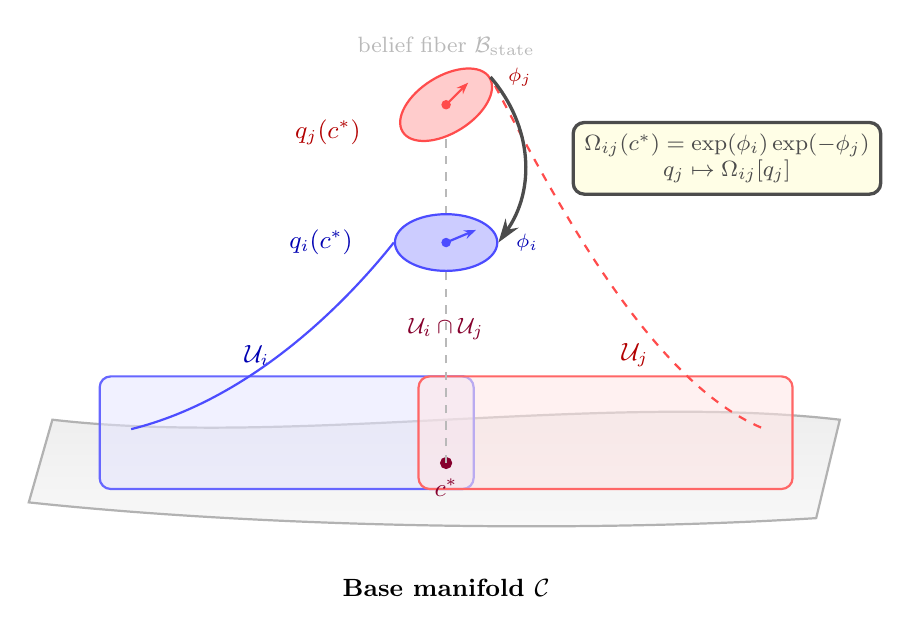
\begin{tikzpicture}[
  >={Stealth[length=2mm]},
  every node/.style={font=\small},
  belief/.style={thick, minimum width=1.3cm, minimum height=0.72cm}
]
\coordinate (base-left) at (0,0);
\coordinate (base-right) at (10,0);
\coordinate (overlap) at (5,-0.55);
\shade[top color=gray!15, bottom color=gray!5, draw=gray!60, thick]
  (base-left) .. controls (3,-0.35) and (7,0.35) .. (base-right)
  -- (9.7,-1.25) .. controls (6.5,-1.45) and (2.5,-1.35) .. (-0.3,-1.05) -- cycle;
\draw[thick, blue!60, fill=blue!10, fill opacity=0.55, rounded corners]
  (0.6,-0.88) rectangle (5.35,0.55);
\draw[thick, red!60, fill=red!10, fill opacity=0.55, rounded corners]
  (4.65,-0.88) rectangle (9.4,0.55);
\node[blue!70!black, font=\small\bfseries] (ui-label) at (2.6,0.82) {$\mathcal{U}_i$};
\node[red!70!black, font=\small\bfseries] (uj-label) at (7.4,0.82) {$\mathcal{U}_j$};
\node[purple!70!black, fill=white, inner sep=1.5pt, font=\footnotesize] (overlap-label) at (5,1.15) {$\mathcal{U}_i \cap \mathcal{U}_j$};
\filldraw[purple!70!black] (overlap) circle (2pt);
\node[below=2pt of overlap, purple!70!black] (cstar-label) {$c^*$};
\node[below=8mm of cstar-label, font=\small\bfseries] (base-label) {Base manifold $\mathcal{C}$};
\draw[thick, dashed, gray!55] (overlap) -- ++(0,5.05) node[above, font=\footnotesize] {belief fiber $\mathcal{B}_{\mathrm{state}}$};
\node[belief, ellipse, draw=blue!70, fill=blue!20] (qi) at (5,2.25) {};
\filldraw[blue!70] (qi.center) circle (1.5pt);
\draw[-{Stealth[length=1.5mm]}, blue!70, thick] (qi.center) -- ++(0.38,0.16);
\node[left=4mm of qi, blue!70!black] (qi-label) {$q_i(c^*)$};
\node[right=1mm of qi, blue!70!black, font=\scriptsize] (phii-label) {$\phi_i$};
\node[belief, ellipse, draw=red!70, fill=red!20, rotate=32] (qj) at (5,4.0) {};
\filldraw[red!70] (qj.center) circle (1.5pt);
\draw[-{Stealth[length=1.5mm]}, red!70, thick] (qj.center) -- ++(0.28,0.28);
\node[left=4mm of qj, red!70!black] (qj-label) {$q_j(c^*)$};
\node[right=1mm of qj, red!70!black, font=\scriptsize] (phij-label) {$\phi_j$};
\draw[thick, blue!70] (1.0,-0.12) .. controls (2.5,0.25) and (3.7,1.45) .. (qi.west);
\draw[thick, red!70, dashed] (9.0,-0.10) .. controls (7.6,0.50) and (6.4,2.75) .. (qj.east);
\draw[-{Stealth[length=3mm,width=2mm]}, very thick, black!70]
  (qj.east) to[bend left=38] node[midway, right=6mm, draw, rounded corners, fill=yellow!10,
  inner sep=4pt, align=center, font=\footnotesize] (transport-label)
  {$\Omega_{ij}(c^*)=\exp(\phi_i)\exp(-\phi_j)$\\$q_j \mapsto \Omega_{ij}[q_j]$} (qi.east);
\end{tikzpicture}
\caption{%
\textbf{Overlapping agent sections and gauge transport.} Agents $i$ and $j$ define Gaussian belief sections over neighborhoods $\mathcal{U}_i$ and $\mathcal{U}_j$ of the base manifold $\mathcal{C}$. At $c^* \in \mathcal{U}_i \cap \mathcal{U}_j$, the beliefs occupy the same statistical fiber but use local frames $\phi_i$ and $\phi_j$. The transport $\Omega_{ij}(c^*)=\exp(\phi_i)\exp(-\phi_j)$ maps $q_j(c^*)$ into agent $i$'s frame before $D_{\mathrm{KL}}(q_i\|\Omega_{ij}[q_j])$ is evaluated. In the zero-dimensional transformer limit the neighborhoods collapse to one base point and the comparison remains entirely within one fiber.
}
\label{fig:bundle_sections_surface}
\end{figure}

\subsection{Cognitive Reference Frames as Gauge Frames}
\label{sec:cognitive_reference_frames}

Lahav and Neemeh~\cite{LahavNeemeh2022, LahavNeemeh2025} argue that phenomenal consciousness is observer-relative the way simultaneity and velocity are observer-relative in special relativity: a cognitive system's experience is a property of that system viewed from its own cognitive frame of reference, not a fact independent of any observer. Their account writes an explicit transformation only for the degenerate case of functionally identical cognitive systems, where it reduces to a delta-function identification (Eqs.~26 and~35 of the 2022 paper), and leaves the transformation law between distinct cognitive frames unspecified. The construction here supplies a mathematically explicit law for the nondegenerate case: each agent $i$ carries a smooth gauge frame field $\phi_i: \mathcal{U}_i \to \mathfrak{g}$ playing the role of its cognitive frame of reference, the transport operator $\Omega_{ij} = \exp(\phi_i)\exp(-\phi_j)$ defined below is the transformation between frames, and the KL divergence $\mathrm{KL}(q_i \| \Omega_{ij}[q_j])$ is a frame-invariant scalar measuring belief disagreement after transport. The canonical structure group $\mathrm{GL}(K_q)$, together with compact $\mathrm{SO}(N)$ initializations or analytic restrictions only when explicitly configured, is a modeling commitment justified on information-geometric grounds in Section~\ref{sec:gauge_group_choice} rather than by Lahav and Neemeh, who invoke the Lorentz transformation only as a structural analogy; Section~\ref{sec:lahav_convergence} develops the correspondence with the caveats it requires, including the limitation that gauge invariance places no constraint on which gauge frame produces which phenomenal quale.

The formal analog with general relativity is then straightforward. Two physicists describing the same spacetime event in coordinates $(t, x, y, z)$ and $(t', x', y', z')$ relate their measurements via a coordinate transformation; two cognitive systems describing the same domain of inquiry $\mathcal{C}$ (an index manifold, not an agent-independent physical substrate; Definition~\ref{def:base_manifold}) in frames $\phi_i$ and $\phi_j$ relate their belief representations via $\Omega_{ij}$. The analog is a working correspondence rather than an identity: the transformation group on the cognitive side is $\mathrm{GL}(K_q)$ (or its $\mathrm{SO}(N)$ subgroup), and the transformations act on probability distributions on a statistical manifold rather than on coordinates of a Lorentzian spacetime. The frame $\phi_i(c)$ specifies the agent's choice of internal axes for representing belief content at base point $c$; it is a field over $\mathcal{C}$ rather than a single matrix because the choice can vary spatially, and it lives in $\mathfrak{g}$ because we want continuous deformations between nearby choices. For $G = \mathrm{SO}(3)$ an instance of $\phi_i$ is an internal rotation; for general $G$ it is a basis change in the agent's representational space, not an orientation in physical space. As a concrete example, two agents perceiving the same colored surface may represent color along different internal bases, agreeing about the spectral content of the stimulus but disagreeing about the components in which they internally represent it; their gauge frames differ by the basis change relating the two schemes, and comparing their beliefs requires transport, after which the residual $\mathrm{KL}(q_i \| \Omega_{ij}[q_j])$ is the part of the disagreement that does not reduce to a basis choice.

\subsubsection{Transport Operators: Translating Between Frames}
\label{sec:transport}

When agents $i$ and $j$ overlap at point $c \in \mathcal{U}_i \cap \mathcal{U}_j$, the inter-agent transport operator is defined as
\begin{equation}
\Omega_{ij}(c) = \exp[\phi_i(c)] \exp[-\phi_j(c)] \in G.
\label{eq:transport_def}
\end{equation}
This group element transforms agent $j$'s representations into agent $i$'s frame, acting on probability distributions through the representation $\rho: G \to \mathrm{Aut}(\mathcal{B})$ as $\Omega_{ij}[q_j](c) := \rho(\Omega_{ij}(c)) q_j(c)$. The product of two exponentials is what gives $\Omega_{ij}$ its range: a single exponential covers only a neighborhood of the identity (Section~\ref{sec:local_trivialization}), whereas the pair $\exp(\phi_i)\exp(-\phi_j)$ realizes all of $\mathrm{GL}^+(K_q)$ for a single pair considered in isolation: by polar decomposition $A = RP$ with $R \in \mathrm{SO}(K_q) = \exp(\mathfrak{so}(K_q))$ and $P$ symmetric positive-definite with $-\phi_j = \log P$, every identity-component element is attained. (Across the coupled system the same $\phi_i$ enters every pair, so the joint transports are constrained to the cocycle family.) The same construction forces $\Omega_{ij}$ to be a genuine relative operator: demanding a single constant, pair-independent transport forces $\Omega^2 = \Omega$ through the cocycle $\Omega_{ij}\Omega_{jk} = \Omega_{ik}$, hence $\Omega = I$ whenever at least three agents are present, and $\Omega = I$ collapses all frames to a common $U$; for exactly two agents only the weaker involution condition $\Omega^2 = I$ survives, admitting nonidentity involutions such as $\Omega = -I$ for even $K_q$. For Gaussian beliefs $q_j = \mathcal{N}(\mu_j, \Sigma_j)$ with $G = \mathrm{SO}(3)$, transport acts through the rotation matrix $R_{ij} = \exp[\phi_i]\exp[-\phi_j]$, transforming $\mu_j \mapsto R_{ij}\mu_j$ and $\Sigma_j \mapsto R_{ij}\Sigma_j R_{ij}^\top$, and the transported belief $\Omega_{ij}[q_j](c)$ represents agent $j$'s belief at $c$ expressed in agent $i$'s coordinate system, enabling the meaningful comparison $\mathrm{KL}(q_i \| \Omega_{ij}[q_j])$.

The vertex-local form of Eq.~\eqref{eq:transport_def} carries an immediate cocycle theorem, invoked throughout the manuscript.

\begin{lemma}[Vanishing Holonomy]
\label{thm:vanishing_holonomy}
For gauge transport of the form $\Omega_{ij} = g_ig_j^{-1}$ with vertex-local group elements $g_i \in G$, the holonomy around any closed loop vanishes:
\begin{equation}
H_{ijk} = \Omega_{ij}\Omega_{jk}\Omega_{ki}
= g_ig_j^{-1}g_jg_k^{-1}g_kg_i^{-1}
= I.
\label{eq:holonomy}
\end{equation}
Equivalently, the cocycle condition $\Omega_{ij}\Omega_{jk} = \Omega_{ik}$ holds for all triples $(i,j,k)$.
\end{lemma}

\begin{proof}
Direct computation. The consecutive inverse-exponential pairs cancel identically: $g_j^{-1} g_j = I$ and $g_k^{-1} g_k = I$.
\end{proof}

This is a cocycle identity following from the vertex-local parameterization $\Omega_{ij} = U_iU_j^{-1}$, not an approximation: semantic transport from agent $i$ to agent $k$ is path-independent regardless of the learned gauge frames $\phi_i$, the direct route via $\Omega_{ik}$ and the indirect route via $\Omega_{ij}\Omega_{jk}$ yielding identical results, and in the gauge-theoretic dictionary the identity expresses the Regime~I flatness whose canonical statement follows in Section~\ref{sec:connection_forms}. Architectures with nontrivial curvature and holonomy require the edge-local connection $\delta_{ij}$ of Section~\ref{sec:discrete_regime_ii}, of which the cocycle here is the special case $\delta_{ij} = 0$.

\subsubsection{Gauge Covariance: The Fundamental Principle}
\label{sec:gauge_covariance_principle}

Two distinct invariances are at play, and we keep them apart. The \emph{global diagonal redundancy} is a single right-translation $U_i \mapsto U_i g$ applied to all agents with the \emph{same} $g \in G$, under which $\Omega_{ij} = U_i U_j^{-1} \mapsto U_i g g^{-1} U_j^{-1} = \Omega_{ij}$ is invariant. This is the redundancy of the overall labeling of the gauge orbit, and the version we use throughout the body when we say the framework is gauge-invariant. The \emph{full local gauge freedom} of a principal bundle is stronger: independent left-translations $U_i \mapsto g_i U_i$ for each agent (the lattice-gauge convention of the discrete Regime~II construction of Section~\ref{sec:discrete_regime_ii}), under which $\Omega_{ij} \mapsto g_i \Omega_{ij} g_j^{-1}$ and $q_j \mapsto \rho(g_j) q_j$ so that $\Omega_{ij} q_j$ acquires $\rho(g_i)$ on the left and the pairwise KL $\mathrm{KL}(q_i \| \Omega_{ij} q_j)$ becomes invariant by KL invariance under common pushforward. The two actions are deliberately different: the global diagonal action is a right-translation so that $\Omega_{ij}$ is pointwise invariant (the strongest redundancy statement), while the full local action is the lattice-gauge left-translation so that $\Omega_{ij}$ transforms as a link variable. The two actions are distinct even in kind: the diagonal redundancy is an action of the single group $G$ by right translation, while the lattice freedom is an action of $G^{|I|}$ by left translation; restricted to the diagonal subgroup the two translations are intertwined only by group inversion, which is not a map of the representation. They coincide on observables (KL pairings and class functions of closed loops) by KL invariance under common pushforward. Under the full local action every KL term of the functional~\eqref{eq:free_energy_functional_final} is invariant by common pushforward (Theorem~\ref{thm:glk_invariance}), and the attention and meta entropies are invariant because $\beta$ and $\gamma$ are functions of those KLs; the functional as a whole is invariant exactly when all statistical fields, including the observation model and any frozen hyper-prior, are transformed together, and fails to be invariant only when a fixed field is exempted from the action. We use the global diagonal redundancy as the working notion because the implementation holds the observation channel fixed.

The consequence of the global diagonal redundancy is that only relative gauge frames matter. Individual frames $\phi_i$ carry the two roles (A and B) of Section~\ref{sec:agents_as_sections}, and we use gauge-invariant for quantities unchanged under both the global diagonal redundancy and the full local gauge action, while gauge-covariant is reserved for quantities transforming according to a specified representation. The single most consequential downstream use of this distinction is the Lahav-Neemeh Alice/Bob correspondence (Section~\ref{sec:lahav_convergence}), a composition of two transports of the form $\Omega_{ab} = \exp(\phi_a)\exp(-\phi_b)$ obeying the cocycle/transitivity property $\Omega_{ik} = \Omega_{ij}\Omega_{jk}$ in which the inter-agent factor lives in the global-diagonal sector and the cross-scale factor in the full local action; its covariance-sector reading would not survive if the two senses were not held apart. The Lie-algebra additive form $\phi_i \mapsto \phi_i + \xi$ coincides with the group-level form only when $\xi$ commutes with each $\phi_i$, since the Baker-Campbell-Hausdorff expansion $\exp(\phi_i + \xi) = \exp(\phi_i)\exp(\xi)\exp(-\tfrac12 [\phi_i, \xi])\cdots$ collapses to $\exp(\phi_i)\exp(\xi)$ only when the commutator vanishes; the additive shift is the genuine gauge transformation only for abelian groups or central $\xi$, and for the non-abelian groups used here the group-level form $U_i \mapsto U_i g$ is the correct statement of the global redundancy. The relative pairing $U_i U_j^{-1}$ is thus gauge-invariant under the global diagonal action and gauge-covariant under the agent-wise lattice-gauge action, just as in general relativity individual coordinate systems are arbitrary while coordinate-invariant quantities like proper time are physically meaningful.

\subsubsection{Connection Forms and Parallel Transport}
\label{sec:connection_forms}

Under the Regime~I / Regime~II convention fixed at the head of this section, the connection-form discussion below develops the general gauge-theoretic vocabulary that becomes dynamically nontrivial only after the Regime~II promotion. The gauge frame $\phi_i$ induces a Lie-algebra-valued one-form on agent $i$'s domain,
\begin{equation}
\theta^{(i)}_\mu(c) := U_i^{-1}(c) \partial_\mu U_i(c) \in \mathfrak{g},
\label{eq:connection_form}
\end{equation}
where $U_i(c) = \exp[\phi_i(c)] \in G$ and $\partial_\mu = \partial/\partial c^\mu$. This is the left Maurer-Cartan frame-gradient pulled back along the agent's local section $U_i: \mathcal{U}_i \to G$ on the trivializing patch $\mathcal{U}_i$, not a dynamical Yang-Mills connection: under the cocycle parameterization $\Omega_{ij} = U_i U_j^{-1}$ the curvature $d\theta + \theta \wedge \theta$ vanishes identically. This is the canonical statement of Regime~I flatness, established once here and assumed thereafter. We retain the symbol $A^{(i)}_\mu$ for $\theta^{(i)}_\mu$ throughout when the context is the frame-gradient reading; the Yang-Mills reading, in which $A$ is an independent connection variable, is the Regime~II extension. On overlapping regions the relation between the two agents' frame-gradients follows from $U_i = \Omega_{ij} U_j$ and the chain rule,
\begin{equation}
\theta^{(i)}_\mu = \mathrm{Ad}(U_j^{-1})\big[\Omega_{ij}^{-1} \partial_\mu \Omega_{ij}\big] + \theta^{(j)}_\mu,
\label{eq:theta_overlap_relation}
\end{equation}
where $\mathrm{Ad}(U_j^{-1})$ is the adjoint action of $U_j^{-1}$ on $\mathfrak{g}$. Equation~\eqref{eq:theta_overlap_relation} is \emph{not} the standard Yang-Mills gauge-transformation law $A^{(i)} = g A^{(j)} g^{-1} - (dg) g^{-1}$, which holds for an independent connection variable; the mismatch reflects that $\theta = U^{-1}dU$ is the pullback of a frame-gradient, not a section-independent gauge potential. Under Regime~II the Yang-Mills law is recovered, but in Regime~I Eq.~\eqref{eq:theta_overlap_relation} is the correct overlap relation.

\subsubsection{Gauge Field Strength: Path-Dependent Information Transport}
\label{sec:field_strength}

The field strength (curvature two-form) measures the path-dependence of parallel transport,
\begin{equation}
F^{(i)}_{\mu\nu}(c) = \partial_\mu A^{(i)}_\nu - \partial_\nu A^{(i)}_\mu + [A^{(i)}_\mu, A^{(i)}_\nu] \in \mathfrak{g}.
\label{eq:field_strength}
\end{equation}
\emph{This subsubsection is Regime~II content.} Under Regime~I the connection inherits the pure-gauge form $A = U^{-1}dU$, the Maurer-Cartan identity forces $F^{(i)}_{\mu\nu} = 0$ identically (Section~\ref{sec:connection_forms}), and parallel transport around any closed loop returns the original belief unchanged. In Regime~II a non-zero $F^{(i)}_{\mu\nu}$ creates path-dependent information transport: beliefs accumulate holonomy around closed loops, with the net transformation depending on the enclosed area. The cognitive interpretation is that the agent's internal coordinate system is twisted across the base manifold so that different paths through conceptual space lead to different final orientations, analogous to parallel-transporting a vector around a curved surface; an agent walking a closed triangle near the north pole and always walking straight returns rotated relative to its starting orientation, which is holonomy encoded in $F_{\mu\nu}$. None of this is dynamically active in the Regime~I implementation, but the construction is retained because the framework's gravitational and signature-related extrapolations require it.

\subsubsection{Discrete Regime~II via an Edge-Relaxed Cocycle}
\label{sec:discrete_regime_ii}

The continuous Regime~II description, an independent connection $A^{(i)}_\mu$ and a path-ordered exponential $\Omega_\gamma = \mathcal{P}\exp(-\int_\gamma A_\mu dx^\mu)$, has a natural discrete realization on the agent graph compatible with the vertex-frame skeleton. Beginning from the cocycle parameterization $\Omega_{ij} = U_iU_j^{-1}$ of Regime~I, one introduces an edge-local connection variable $\delta_{ij} \in \mathbb{R}^{n_{\mathrm{gen}}}$ valued in the Lie-algebra coordinates and writes
\begin{equation}
\Omega_{ij} = U_i \exp\big(\delta_{ij}\cdot G\big) U_j^{-1},
\qquad
\delta_{ij}\cdot G \equiv \sum_{a=1}^{n_{\mathrm{gen}}} \delta_{ij}^{a} G_a \in \mathfrak{g},
\label{eq:edge_relaxed_omega}
\end{equation}
with $\{G_a\}$ the structure-group generators. Setting $\delta_{ij}=0$ recovers the Regime~I cocycle and the vanishing-holonomy lemma; allowing $\delta_{ij}\neq 0$ admits nontrivial holonomy on closed cycles. Equation~\eqref{eq:edge_relaxed_omega} is the standard lattice-gauge-theory link variable~\cite{WilsonConfinement1974, KogutSusskind1975, Creutz1983} written in a vertex-trivialized parameterization that exposes the Regime~I skeleton as a special case. Under a vertex-local gauge transformation $U_i \to g_i U_i$ the transport transforms by left-conjugation at the source and right-conjugation at the target,
\begin{equation}
\Omega_{ij} \longmapsto g_i \Omega_{ij} g_j^{-1},
\label{eq:omega_gauge_law}
\end{equation}
matching the lattice-gauge transformation law for link variables~\cite[Eq.~12]{WilsonConfinement1974},~\cite[ch.~5 Eq.~5.1]{Creutz1983}: $\Omega_{ij}$ is gauge-covariant, not gauge-invariant. The connection coefficients $\delta_{ij}$ are invariant under the chosen lift in which $U_i \mapsto g_i U_i$ is absorbed entirely into the vertex factors and the central $\exp(\delta_{ij}\cdot G)$ is left untouched; this is invariance of a gauge-slice representative rather than of a physical observable, and gauge-invariant observables of the connection require closed-loop traces. This formal index-space lattice gauge on the agent graph, under which per-agent frame relabelings are a gauge-slice redundancy and only closed-loop holonomies are observable, is distinct from the base-local physical gauge $h(c)$ of Appendix~\ref{sec:meta_agent_rg}, under which per-agent frame differences are epistemically physical (the irreducible disagreement $\mathrm{KL}(q_i \| \Omega_{ij}q_j)$); the two senses are reconciled there, and only the base-local action is the framework's physical gauge group.

Around a 3-cycle $i\to j\to k\to i$ on the agent graph, the holonomy is
\begin{equation}
H_{ijk}
:= \Omega_{ij}\Omega_{jk}\Omega_{ki}
= U_i \cdot \exp(\delta_{ij}\cdot G) \exp(\delta_{jk}\cdot G) \exp(\delta_{ki}\cdot G) \cdot U_i^{-1},
\label{eq:discrete_holonomy}
\end{equation}
with the interior vertex factors $U_jU_j^{-1}$ and $U_kU_k^{-1}$ collapsing as in the vanishing-holonomy lemma. Under the gauge transformation~\eqref{eq:omega_gauge_law}, $H_{ijk} \to g_i H_{ijk} g_i^{-1}$ is conjugated at the base point, so the trace
\begin{equation}
W_{ijk} := \operatorname{Re}\operatorname{Tr}(H_{ijk})
= \operatorname{Re}\operatorname{Tr}\big[\exp(\delta_{ij}\cdot G) \exp(\delta_{jk}\cdot G) \exp(\delta_{ki}\cdot G)\big],
\label{eq:wilson_observable}
\end{equation}
is the gauge-invariant Wilson observable in the Regime~II extension. The corresponding Wilson-style holonomy-penalty regularizer, driving the field toward Regime~I, is
\begin{equation}
S_{\mathrm{Wilson}}[\delta]
= \beta \sum_{(i,j,k)} \Big(1 - \tfrac{1}{K_q} W_{ijk}\Big),
\qquad
\beta \to \infty \Longrightarrow H_{ijk} \to I,
\label{eq:wilson_action}
\end{equation}
where $K_q$ is the dimension of the defining representation. For compact $G$ (for example $\mathrm{SO}(N)$), $\operatorname{Re}\operatorname{Tr}(H_{ijk})\le K_q$ with equality only at the identity, so the compact Wilson-trace action is nonnegative and minimized at $H_{ijk}=I$. This conclusion does not extend to noncompact $\mathrm{GL}^+(K_q)$, where the trace action is unbounded below. The conjugacy-invariant eigenvalue deviation
\begin{equation}
d_{\mathrm{ss}}(H):=\sum_a|\lambda_a(H)-1|
\end{equation}
is only a semisimple diagnostic. For
\begin{equation}
H_t=\begin{pmatrix}1&t\\0&1\end{pmatrix},\qquad t\ne0,
\end{equation}
both eigenvalues equal one although $H_t\ne I$, so $d_{\mathrm{ss}}(H_t)=0$. The Frobenius frame-metric penalty detects the same shear, $\|H_t-I\|_F^2=t^2\ge0$, but it is not invariant under general conjugation: for $g=\operatorname{diag}(a,a^{-1})$, $\|gH_tg^{-1}-I\|_F^2=a^4t^2$. For $K_q\geq2$, no continuous conjugacy-invariant function of holonomy alone can be both faithful and zero only at $I$ on all of $\mathrm{GL}^+(K_q)$, because a nonidentity unipotent shear, embedded as a $2\times2$ block when $K_q>2$, can be conjugated along an orbit that accumulates at the identity. The one-dimensional group $\mathrm{GL}^+(1)=\mathbb{R}_{>0}$ is an exception: $|H-1|$ is continuous, conjugacy-invariant, and vanishes only at the identity. The checked-in multi-agent configuration selects \texttt{ym\_bounded=True} with the default \texttt{ym\_action\_form='frobenius'}; it therefore uses a nonnegative Frobenius frame-metric plaquette penalty, while the eigenvalue quantity remains a separately labeled semisimple diagnostic. Its active pairwise attention transport is the Regime~I vertex cocycle; the independent pairwise Regime~II connection is inactive. A scalar relaxation parameter $\alpha\in[0,1]$ in $\Omega_{ij}(\alpha)=U_i\exp(\alpha\delta_{ij}\cdot G)U_j^{-1}$ remains a theoretical interpolation between Regime~I and an edge-relaxed Regime~II.

The autoregressive causal attention mask defines a directed acyclic graph on the token sequence: closed loops in the data flow do not exist, and the holonomy~\eqref{eq:discrete_holonomy} is a property of the connection field $\delta_{ij}$ as a tensor on the index space rather than of the actual message-passing pattern. In bidirectional or encoder attention the underlying graph admits closed loops and the Wilson observable~\eqref{eq:wilson_observable} acquires direct dynamical content, so the clearest experimental test of the gauge-curvature linguistic conjecture (Section~\ref{sec:discussion}) lives in bidirectional architectures where the holonomy is not a purely formal index-space invariant. The connection $\delta_{ij}$ admits two parameterizations. As a free variable per ordered pair it gives textbook lattice gauge theory with the standard Wilson plaquette action; as a learnable function $\delta_{ij} = f_W(\mu_i, \mu_j)$ of the local belief means it yields a \emph{data-dependent} gauge field, the connection itself a function on the data manifold and the regularizer~\eqref{eq:wilson_action} the empirical estimator of $\mathbb{E}_{\mathrm{data}}[S_{\mathrm{Wilson}}]$. We call this a Wilson-style holonomy-penalty action rather than a Yang-Mills action, a discrete plaquette regularizer conditional on the Regime~II promotion, and do not assert a continuum Yang-Mills field theory. In the companion transformer codebase (\texttt{V3\_Transformer}) the connection is parameterized via a learnable belief-mean-conditioned bilinear $\delta_{ij}^a = \mu_i^\top W^a \mu_j$ or a small feedforward map on the concatenated means, both seeing inputs in the embedding ambient frame rather than a per-vertex rotated frame; full per-vertex equivariance, passing $U_i^{-1}\mu_i$ rather than $\mu_i$, is a separate architectural commitment beyond the scope formalized here. The multi-agent reference implementation, by contrast, carries a state-independent lattice connection whose edge twists $V_{ij}$ are set by \texttt{init\_twist\_scale} and do not depend on the belief means. For multi-head attention restricted to the block-diagonal subgroup $\mathrm{GL}(d_{\mathrm{head}})^H \subset \mathrm{GL}(d_{\mathrm{model}})$ (Section~\ref{sec:transformers}), each head carries its own connection $\delta_{ij}^{(h)}$ in its own irrep block, and the holonomy decomposes as a direct sum $H_{ijk} = \bigoplus_h H_{ijk}^{(h)}$. The Wilson trace observable adds across heads, while the squared Frobenius penalty adds in squared norms and the Frobenius norm itself combines by root-sum-of-squares; aggregate diagnostics over the full block-diagonal representation therefore require slicing by head to recover the per-head decomposition. In the Regime~I implementation realized here the connection is pure-gauge and curvature vanishes identically, so these holonomy diagnostics are degenerate.

\subsection{The Hierarchy of Transport Operators}
\label{sec:transport_hierarchy}

The full multi-agent, multi-scale structure requires several distinct types of information transport. Intra-scale belief transport $\Omega_{ij}: \mathcal{B}_{\mathrm{state}} \to \mathcal{B}_{\mathrm{state}}$ is the primary operator of Eq.~\eqref{eq:transport_def}, transporting agent $j$'s belief into agent $i$'s gauge frame within the same hierarchical level; because $p$ and $q$ both inhabit $\mathcal{B}_{\mathrm{state}}$, the same operator transports priors, and we use a single symbol $\Omega_{ij}$ for both. The model-coupling term $\gamma_{ij}\mathrm{KL}(s_i\|\tilde{\Omega}_{ij}s_j)$ uses the model-fiber transport $\tilde{\Omega}_{ij}: \mathcal{B}_{\mathrm{model}} \to \mathcal{B}_{\mathrm{model}}$, equal to $\Omega_{ij}$ as a group element but acting on a different fiber; since hyper-priors $r$ and generative models $s$ both inhabit $\mathcal{B}_{\mathrm{model}}$, $\tilde{\Omega}_{ij}$ also transports hyper-priors. Cross-scale transport requires additional operators connecting hierarchical levels: bottom-up transport $\Lambda^{s \to s+1}$ aggregates constituent beliefs upward when forming meta-agent $I$ at scale $(s{+}1)$ through gauge-covariant averaging (Section~\ref{sec:meta_agent_formation}), with a model-channel analog aggregating constituent generative models, while top-down transport in the reverse direction propagates meta-level information back to constituents, providing the cross-scale shadows of Eq.~\eqref{eq:cross_scale_shadow} and realizing top-down participatory feedback.

The constituent-meta-agent transport $\Omega_{i,I} = \exp(\phi_i^{(s)})\exp(-\phi_I^{(s+1)})$ used for top-down prior propagation, and implicitly in the bottom-up aggregation that builds $\bar{\mu}_I$ and $\bar{\Sigma}_I$ from the transported constituent beliefs, is a special case of the general inter-agent law $\Omega_{ab} = \exp(\phi_a)\exp(-\phi_b)$ with $a$ and $b$ allowed to live at different scales. This works because the meta-agent frame construction $\phi_I^{(s+1)}(x) = \sum_{i \in I} w_i(x)\phi_i^{(s)}(x) / \sum_{i \in I} w_i(x)$ (Section~\ref{sec:meta_agent_formation}) keeps $\phi_I^{(s+1)}$ in the same Lie algebra $\mathfrak{g}$ as the constituent frames, so $\exp(\phi_a)\exp(-\phi_b)$ is a well-defined product of two group elements whether $a$ and $b$ are intra-scale or cross-scale. Intra-scale and cross-scale gauge transformations are unified under the same group action, and the pan-agentic commitment of Section~\ref{sec:introduction} makes this unification structural rather than merely notational (the Baker-Campbell-Hausdorff accuracy bound and the noncompact $\mathrm{GL}^+(K_q)$ caveat on this average are in Section~\ref{sec:meta_agent_variational}).

\subsection{Curvature Structure: Four Interacting Geometries}

The framework involves four distinct notions of curvature, whose interplay underwrites its emergent-geometry reading. \emph{Statistical-manifold curvature} governs fiber geometry: the fiber $\mathcal{B}$ is itself a curved Riemannian manifold, and the manifold of Gaussian distributions under the Fisher-Rao metric has sectional curvature of \emph{mixed sign} for $K_q \geq 2$~\cite{Skovgaard1984}. The SPD covariance sector $\mathbb{S}^+_{K_q}$ is a Riemannian symmetric space of nonpositive curvature, and the univariate case and the location-scale family with fixed correlation reduce to hyperbolic geometry of constant negative curvature, but the full joint mean-covariance manifold admits 2-planes of strictly positive curvature (for orthonormal pure-mean directions at $\Sigma = I$ the sectional curvature equals $+1/4$); uncertainty diverges along the nonpositively curved covariance directions while mean-direction planes can be positively curved, and this fiber curvature governs natural-gradient flow within each fiber. \emph{Gauge-group curvature} reflects frame-space geometry: the structure group $G$ is itself a curved manifold, with $\mathrm{SO}(3) \cong \mathbb{RP}^3$ carrying constant positive curvature, and is non-commutative, so the order of unrelated transports matters ($\Omega_{ab}\Omega_{cd} \neq \Omega_{cd}\Omega_{ab}$ for disjoint pairs). For chained transports through a common intermediate agent, however, the cocycle $\Omega_{ij}\Omega_{jk} = \Omega_{ik}$ holds identically by the algebraic collapse $U_j^{-1}U_j = I$ regardless of commutativity, so the vertex-local parameterization used here is automatically flat. \emph{Gauge-field curvature} characterizes connection geometry: the field strength $F^{(i)}_{\mu\nu}$ measures how the agent's frame twists across $\mathcal{C}$, and in Regime~I it vanishes identically (Section~\ref{sec:connection_forms}), so this curvature carries no dynamical content in the present implementation; the non-zero $F_{\mu\nu}$ envisaged where moving beliefs along different paths yields different results is a Regime~II construct, the structural counterpart of the Yang-Mills field strength of gauge bosons. \emph{Base-manifold curvature} represents substrate geometry: if $\mathcal{C}$ carries an intrinsic metric its Riemann tensor affects geodesics in the noumenal substrate, but in our framework $\mathcal{C}$ typically has no preferred metric a priori, metrics being induced by agent beliefs through pullback (Section~\ref{sec:pullback}). These four interact: fiber curvature shapes belief dynamics along natural-gradient flow, group curvature determines how gauge transformations compose and so influences holonomy around loops, the frame-twist horizontal block built from the connection couples the agent's gauge frame to the induced base geometry through the pullback (with $F_{\mu\nu}$ entering this coupling only after the Regime~II promotion, since $F_{\mu\nu} = 0$ in Regime~I), and induced base curvature feeds back into how beliefs propagate spatially. This structure underwrites the framework's spacetime-phenomenology reading, in which curvature-like structures arise from the information-geometric dynamics of coupled agents while their identification with physical gravity is treated as an open program (Section~\ref{sec:open_problems}) rather than a derivation.

\subsection{Working Framework: Simplifications and Scope}
\label{sec:working_framework}

The general framework above is rich but computationally intensive, and for this study we adopt several simplifications that preserve the essential geometric structure while ensuring tractability. These are practical implementation choices, not theoretical limitations; the full framework remains available for future investigation. One structural fact and four simplifications frame the working realization. The structural fact: beliefs and priors share the latent-state manifold $\mathcal{B}_{\mathrm{state}}$, and generative models and hyper-priors share the model-parameter manifold $\mathcal{B}_{\mathrm{model}}$, both \emph{by construction} from the cross-scale shadow relation~\eqref{eq:cross_scale_shadow} rather than as separate assumptions, so the shared-manifold property is a structural commitment of the framework (Section~\ref{sec:cross_scale_shadows}). The four practical restrictions follow. Both fibers are Gaussian. The canonical gauge group is $G = \mathrm{GL}(K_q, \mathbb{R})$ acting on the belief fiber, with a separate complex $\mathrm{GL}(K_q, \mathbb{C})$ acting on the gauge connection only (Section~\ref{sec:signature_resolution}); the compact subgroups $\mathrm{SO}(N) \subset \mathrm{GL}(N)$, including $\mathrm{SO}(3)$ realized as three-dimensional rotations, are studied as special cases for analytical and proof-of-concept clarity. The base manifold is flat, $\mathcal{C} = \mathbb{R}^2$ with Euclidean geometry. Gauge frames are smooth and slowly varying, so the Maurer-Cartan frame-gradient $A^{(i)}_\mu = U_i^{-1}\partial_\mu U_i$ is small and the first-order Baker-Campbell-Hausdorff frame averaging of Section~\ref{sec:meta_agent_formation} is accurate; the field strength vanishes identically in Regime~I independently of this hypothesis and of the variation rate (Section~\ref{sec:connection_forms}).

These choices are motivated by computational feasibility (closed-form KL divergences, efficient $\mathrm{SO}(3)$ operations), analytical tractability (known curvature of Gaussian manifolds), physical interpretability ($\mathrm{SO}(3)$ familiar from spatial rotations), and proof-of-concept scope. They preserve gauge covariance with nontrivial transport operators, information-geometric dynamics via Fisher metrics, multi-scale hierarchical emergence, curved statistical manifolds, and non-commutative gauge-group structure; they sacrifice path-dependent parallel transport (holonomy), non-Gaussian belief structures, heterogeneous agent types, curved base-manifold geometry, and gauge-field curvature $F_{\mu\nu}$ altogether (Regime~I flatness).

\begin{table*}[t]
\centering
\small
\caption{Executable contract and scope of the constructions used in this manuscript. ``Active'' refers to the checked-in \texttt{CONFIG} after loader normalization, not to a constructor default considered in isolation.}
\label{tab:executable_contract}
\begin{tabularx}{\textwidth}{@{}p{0.22\textwidth}X@{}}
\toprule
Subject & Scope-separated contract \\
\midrule
Covariance flow & \textbf{Theoretical/pure and opt-in:} the full affine-invariant Gaussian covariance natural gradient with an SPD exponential retraction. \textbf{Active:} \texttt{sigma\_natural\_gradient=False}, so covariance parameters receive Euclidean descent through their Cholesky factors, with an SPD-Fisher trust-region bound. \\
E/M semantics & \textbf{Formal:} the fast-belief and slow-model decomposition admits a block E/M interpretation. \textbf{Active:} one scalar backward pass drives simultaneous, rate-separated descent on the joint product manifold; \texttt{model\_lr\_ratio=0.01} supplies separation but not block-coordinate optimization. \\
Connection and action & \textbf{Active:} pairwise matter alignment uses the Regime-I vertex cocycle $\Omega_{ij}=U_iU_j^{-1}$, while a separate lattice field contributes the configured Frobenius self-action. \textbf{Opt-in/test-only:} independent pairwise connection transport. The checked-in pairwise twist scale and learning rate are zero, so that path is inactive. \\
Pullback and training metric & \textbf{Implemented diagnostic:} the fixed-gauge ordinary Gaussian Fisher pullback, with an optional indefinite horizontal trace tensor. \textbf{Active training:} the frame update uses the Frobenius body covector; the pullback helper is opt-in and is not the default training metric. \\
Frame group & \textbf{Historical:} the superseded emergence simulator used spin-$\ell$ representations of $\mathrm{SO}(3)$. \textbf{Active:} smooth initialization exponentiates skew $7\times7$ fields and therefore starts in $\mathrm{SO}(7)$; subsequent unconstrained $\mathfrak{gl}(7)$ retractions evolve in $\mathrm{GL}^+(7)$. \textbf{Reusable construction:} \texttt{Agent} permits general $\mathrm{GL}^+(K)$ initialization. \\
Consensus quantity & \textbf{Implemented:} consensus scores and coherence quantities are detector or diagnostic outputs. \textbf{Historical/prospective:} their use as thermodynamic order parameters is a proposed interpretation, not an empirically demonstrated phase observable in the recoverable evidence. \\
Precision hierarchy & \textbf{Active:} scalar adaptive precision is evaluated with fixed $b_0,c_0$; the loader rejects learned precision hyperparameters. \textbf{Prospective:} per-coordinate or per-head gains and a normalized learned Gamma hierarchy with proper hyper-hyperpriors. \\
\bottomrule
\end{tabularx}
\end{table*}

\paragraph{Matched bundles on the two-manifold structure.}
By construction (Eq.~\eqref{eq:cross_scale_shadow}), beliefs and priors share the latent-state manifold $\mathcal{B}_{\mathrm{state}} =: \mathcal{B}$ and representation $\rho_{\mathrm{state}} =: \rho$ with a single associated bundle $\mathcal{E}_{\mathrm{state}} =: \mathcal{E}$, and generative models and hyper-priors analogously share $\mathcal{B}_{\mathrm{model}}$ and $\mathcal{E}_{\mathrm{model}}$; setting the slow subsystem aside, each agent $i$ is represented by a single section $\sigma^i: \mathcal{U}_i \to \mathcal{E}$ carrying $\sigma^i(c) = (q_i(c), p_i(c))$. This is reasonable because beliefs and priors are both probability distributions over the same underlying space, distinguished by separate components rather than separate bundle structure; what is sacrificed is the ability to model qualitatively different belief and prior types, for example Gaussian beliefs with categorical priors, a heterogeneity inessential to demonstrating emergent structure here. Equivalently, the canonical functional~\eqref{eq:free_energy_functional_final} contains no cross-bundle morphism coupling the model and belief channels; the two channels couple only through the gauge-frame sector and the within-channel cross-scale shadows of Eq.~\eqref{eq:cross_scale_shadow}. In the shared-frame configuration $\Omega_{ij}$ and $\tilde{\Omega}_{ij}$ act as the same element of $G$ in two representations; in the independent-frame configuration of the reference implementation the model fiber carries its own $\mathrm{GL}(K_m)$ bundle and frame field $\tilde{\phi}_i$ (the option following Eq.~\eqref{eq:envelope_gradient_model}), $\tilde{\Omega}_{ij}$ becomes an independent transport, and even the structure-group identification is absent, leaving the cross-scale shadows as the only inter-channel coupling.

\paragraph{Gaussian probability manifold.}
The fiber is $\mathcal{B} = \{\mathcal{N}(\mu, \Sigma) : \mu \in \mathbb{R}^{K_q}, \Sigma \in \mathbb{S}^+_{K_q}\}$, of mixed-sign sectional curvature for $K_q \geq 2$~\cite{Skovgaard1984}, dimension $K_q(K_q+3)/2$, and KL divergence in the closed form of Eq.~\eqref{eq:gaussian_kl}. Gaussians are the maximum-entropy distribution for given mean and covariance, with closed-form expressions enabling efficient computation and a well-studied information geometry. Multivariate Gaussians are a \emph{simplifying choice} rather than a theoretical requirement (Section~\ref{sec:statistical_manifolds}): the gauge-theoretic framework extends to a non-Gaussian exponential-family fiber only after specifying a common bijective sample-space action that preserves that family and leaves the chosen divergence computable. The Gaussian theorem below supplies this closure for affine pushforwards of Gaussian states; mixture models, heavy-tailed distributions, and density-operator fibers require separate closure and computation proofs. A strictly separate complex/quantum fiber with complex-valued amplitudes is a separate program flagged as future work (Section~\ref{sec:open_problems}).

\paragraph{Gauge group: $\mathrm{GL}(K_q)$ as natural symmetry, $\mathrm{SO}(3)$ as computational choice.}
\label{sec:gauge_group_choice}
The full Gaussian family on $\mathbb{R}^{K_q}$ is preserved under the affine group $x \mapsto Ax + b$ with $A \in \mathrm{GL}(K_q)$, $b \in \mathbb{R}^{K_q}$, and the KL divergence (indeed all $f$-divergences) is invariant under any common bijective change of variables since the Jacobian factors cancel in the density ratio. Restricting to the origin-preserving linear subgroup $G = \mathrm{GL}(K_q) \subset \mathrm{Aff}(K_q)$, equivalently treating mean vectors as frame coordinates rather than elements of an affine space with translation freedom, gives the working gauge group. This is a modeling choice: $\mathrm{GL}(K_q)$ is the symmetry of the bilinear attention reduction (Section~\ref{sec:transformers}) and the linear sector of the natural Gaussian symmetry, but not the natural symmetry in the strongest sense, and the translation sector $b$, which would correspond to gauge-equivariant biases on agent means, is flagged as available without being invoked. The invariance theorem below is the standard linear-pushforward statement~\cite{Amari2016}.

\begin{theorem}[$\mathrm{GL}(K_q)$ Gauge Invariance]
\label{thm:glk_invariance}
For any two Gaussian distributions $P = \mathcal{N}(\mu_P, \Sigma_P)$ and $Q = \mathcal{N}(\mu_Q, \Sigma_Q)$ on $\mathbb{R}^{K_q}$, and any invertible linear transformation $\Omega \in \mathrm{GL}(K_q)$, the KL divergence is invariant under simultaneous push-forward:
\begin{equation}
D_{\mathrm{KL}}(\Omega_* P \| \Omega_* Q) = D_{\mathrm{KL}}(P \| Q),
\label{eq:glk_invariance}
\end{equation}
where $\Omega_* P = \mathcal{N}(\Omega\mu_P, \Omega\Sigma_P\Omega^\top)$ denotes the pushforward of $P$ under $\Omega$. We assume $\Sigma_P, \Sigma_Q \succ 0$ throughout; the pushforward $\Omega\Sigma\Omega^\top$ remains positive-definite by Sylvester's law of inertia for $\Omega$ invertible. Singular $\Omega$ ($\det\Omega = 0$) is excluded by the gauge-group assumption $\Omega \in \mathrm{GL}(K_q)$, which would otherwise make the pushforward degenerate.
\end{theorem}

\begin{proof}
We use the Gaussian KL closed form of Eq.~\eqref{eq:gaussian_kl} (recorded again in Appendix~\ref{app:gaussian_kl}). Under the pushforwards $\Omega_* P = \mathcal{N}(\Omega\mu_P, \Omega\Sigma_P\Omega^\top)$ and $\Omega_* Q = \mathcal{N}(\Omega\mu_Q, \Omega\Sigma_Q\Omega^\top)$, the trace term satisfies
\begin{equation}
\mathrm{Tr}\big[(\Omega\Sigma_Q\Omega^\top)^{-1}(\Omega\Sigma_P\Omega^\top)\big] = \mathrm{Tr}\big[\Omega^{-\top}\Sigma_Q^{-1}\Omega^{-1}\Omega\Sigma_P\Omega^\top\big] = \mathrm{Tr}(\Sigma_Q^{-1}\Sigma_P),
\end{equation}
the quadratic term satisfies
\begin{align}
&(\Omega\mu_P - \Omega\mu_Q)^\top (\Omega\Sigma_Q\Omega^\top)^{-1} (\Omega\mu_P - \Omega\mu_Q) \nonumber\\
&= (\mu_P - \mu_Q)^\top \Omega^\top \Omega^{-\top}\Sigma_Q^{-1}\Omega^{-1}\Omega (\mu_P - \mu_Q) = (\mu_P - \mu_Q)^\top \Sigma_Q^{-1}(\mu_P - \mu_Q),
\end{align}
and the log-determinant term satisfies
\begin{equation}
\log\frac{\det(\Omega\Sigma_Q\Omega^\top)}{\det(\Omega\Sigma_P\Omega^\top)} = \log\frac{(\det\Omega)^2 \det\Sigma_Q}{(\det\Omega)^2 \det\Sigma_P} = \log\frac{\det\Sigma_Q}{\det\Sigma_P},
\end{equation}
the $(\det\Omega)^2$ factors canceling identically. Since all three components are invariant,
\begin{equation}
D_{\mathrm{KL}}(\Omega_* P \| \Omega_* Q)
= D_{\mathrm{KL}}(P \| Q).
\end{equation}
\footnote{The reference implementation floors the second-argument covariance by $\epsilon I$ (\texttt{KL\_REGULARISER\_EPS}, default $10^{-4}$). The identity is exact on the pure path $\epsilon=0$ and incurs $O(\epsilon)$ frame-dependent terms at the default floor because the floor is added after transport.}
\end{proof}

The proof extends to all $f$-divergences: for any convex $f$ with $f(1) = 0$,
\begin{equation}
D_f(\Omega_* P \| \Omega_* Q) = D_f(P \| Q), \quad \forall \Omega \in \mathrm{GL}(K_q),
\end{equation}
since the factors $|\det\Omega|$ from the density transformation cancel in the ratio $p(x)/q(x)$. In practice this implies that transport operators need only satisfy $\det(\Omega_{ij}) \neq 0$, and the full $\mathrm{GL}(K_q)$ acts as a gauge symmetry. The exponential parameterization $e^{\phi}$ used throughout restricts to $\det > 0$, since $\det(\exp\phi) = \exp(\mathrm{tr}\phi) > 0$, and the canonical statement of its coverage limitation is this: for $K_q \ge 2$ the real matrix exponential $\exp: \mathfrak{gl}(K_q, \mathbb{R}) \to \mathrm{GL}(K_q, \mathbb{R})$ is \emph{not} surjective onto $\mathrm{GL}^+(K_q, \mathbb{R})$. Its image is the set of matrices admitting a real logarithm, a proper subset of the identity component (matrices with negative real eigenvalues of odd algebraic multiplicity, for instance, fail to admit a real logarithm). The parameterization is therefore sufficient for the implemented dynamics and includes a neighborhood of the identity, but is not a global parameterization of $\mathrm{GL}^+(K_q, \mathbb{R})$; products of two exponentials are required, and by the polar factorization at Eq.~\eqref{eq:transport_def} sufficient, for full coverage of $\mathrm{GL}^+$, and the disconnected components ($\det < 0$) and the missing-logarithm portion of $\mathrm{GL}^+$ are reserved for future study.

The gauge action on Gaussian states is $\rho(\Omega)\cdot(\mu,\Sigma)=(\Omega\mu,\Omega\Sigma\Omega^\top)$. The compact $\mathrm{SO}(3)$ construction supplies a tractable historical specialization, while the canonical Gaussian architecture uses the fundamental representation of $\mathrm{GL}(K_q)$. For belief vectors of dimension $d>3$ with $\mathrm{SO}(3)$ structure, $\rho$ decomposes into irreducibles with $d=\sum_k n_k(2\ell_k+1)$; under $\mathrm{GL}(K_q)$, multi-head structure instead arises as the block-diagonal restriction $\bigoplus_a\mathfrak{gl}(d_{\mathrm{head}})\subset\mathfrak{gl}(K_q)$. The aggregate language-model sweep of Section~\ref{sec:scaling_validation} uses the general $\mathrm{GL}(K_q)$ architecture. The compact multi-scale specialization remains a historical construction rather than recoverable empirical evidence.

\paragraph{Flat base manifold.}
For base-space implementations we use a flat Euclidean background chart, $\mathcal{C} = \mathbb{R}^2$ with $g_{\mathcal{C}} = \delta_{\mu\nu}$. This background metric is a computational convenience for differentiation and support placement rather than an intrinsic property of the noumenal base, which carries no preferred metric of its own; the agent-experienced geometry is the pullback metric induced by beliefs (Section~\ref{sec:pullback}), not $g_{\mathcal{C}}$. Agents may occupy compact support regions $\mathcal{U}_i \subset \mathbb{R}^2$ with periodic boundary conditions to avoid edge effects. The prospective emergence protocol of Section~\ref{sec:participatory} also includes a degenerate zero-dimensional arm ($\dim\mathcal{C}=0$, all agents at a single point), in which coarse-graining is purely informational; no artifact-backed run presently validates that specialization. These choices sacrifice intrinsic curvature of the noumenal substrate, global topological effects, and compact base manifolds without boundary; future work will explore curved base manifolds, particularly hyperbolic spaces $\mathbb{H}^n$ that arise naturally in hierarchical latent representations~\cite{Nickel2017}.

\paragraph{Gauge-covariant KL divergence and the zero-dimensional limit.}
With these simplifications the gauge-aligned KL divergence between agents $i$ and $j$ at point $c$ is $D_{\mathrm{KL}}[q_i(c) \| \Omega_{ij}(c)q_j(c)]$; for Gaussian beliefs the transported belief is $\Omega_{ij}(c)q_j(c) = \mathcal{N}(\Omega_{ij}\mu_j, \Omega_{ij}\Sigma_j\Omega_{ij}^\top)$ with $\Omega_{ij}$ taking values in $\mathrm{GL}^+(K_q)$, while compact $\mathrm{SO}(N)$ restrictions define separate constrained cases. By Theorem~\ref{thm:glk_invariance} this divergence is invariant under simultaneous gauge transformation of both arguments, so belief comparisons are meaningful once agent $j$'s belief is transported into agent $i$'s frame. An important special case occurs when the base manifold collapses to a single point ($\dim\mathcal{C} = 0$) and the gauge connection becomes constant: all frames become position-independent $\phi_i(c) = \phi_i$, connections and curvature vanish, $A_\mu = F_{\mu\nu} = 0$, and the integral over $\mathcal{C}$ reduces to evaluation at a single point. The framework becomes a zero-dimensional gauge theory in this limit, and the mixture-of-sources derivation recovers standard transformer attention through the two complementary routes of Section~\ref{sec:transformers}; the unreduced $\mathrm{GL}(K_q)$ gauge theory on a single point is validated as a working language model there, trained without learned $W_Q/W_K/W_V$ projections, MLPs, or pointwise activations (the sweep configuration retaining a learned post-attention output projection $W_O$ and layer normalization).

Even with these simplifications, the implemented rung supports nontrivial gauge transport between agents, information-geometric dynamics on curved statistical manifolds, multi-scale meta-agent emergence through consensus detection, and top-down participatory feedback. Its validation scope is the Level-1/Level-2 portion of this list (Section~\ref{sec:epistemic_status}); the induced-metric structures on the base manifold (Section~\ref{sec:pullback}), the dimensional decomposition, and the signature mechanism it additionally admits are Level-3 mathematical constructions. With the rung's geometry fixed, the next section equips it with the functional whose minimization drives everything that follows.

\section{The Single-Scale Free Energy Functional}\label{sec:free_energy}

A single agent that minimizes the variational free energy $F[q] = \mathbb{E}_{q}[\log q(x) - \log p(o, x)] \geq -\log p(o)$ performs standard Bayesian inference: the bound is tight when $q$ matches the true posterior, and the functional decomposes into a complexity term $\mathrm{KL}(q \| p)$ that anchors beliefs to the prior and an accuracy term $-\mathbb{E}_{q}[\log p(o \mid x)]$ that rewards explaining observations~\cite{Friston2010, parr2022active} (full preliminaries in Appendix~\ref{app:variational_prelim}). The remainder of this section develops the multi-agent extension of this single-agent functional, derives its inter-agent coupling and softmax attention weights from a consensus-energy construction, and assembles the complete free energy that the dynamics of the rest of the paper minimize.

\subsection{Multi-Agent Extension: From Single Inference to Collective Dynamics}

The functional developed below is a novel multi-agent extension of Friston's single-agent free energy: the inter-agent belief-coupling terms $\sum_{ij}\beta_{ij}\mathrm{KL}(q_i\|\Omega_{ij}q_j)$, the attention-entropy term $\tau\beta_{ij}\log(\beta_{ij}/\pi_{ij})$, and the model-channel analog with $\gamma$ are not present in closed variational form with an inter-frame transport law in the standard free-energy-principle literature~\cite{Friston2010, parr2022active}. The closest precedent is federated inference and belief sharing~\cite{friston2024federated}, in which an agent treats a neighbor's broadcast posterior as an observation and integrates it by variational updating with precision deciding whom to attend to; the present coupling is structurally analogous. In the flat-connection limit $\Omega_{ij} = I$ the alignment block satisfies $\sum_j \beta_{ij}\mathrm{KL}(q_i\|q_j) = -H(q_i) - \sum_j \beta_{ij}\mathbb{E}_{q_i}[\log q_j]$, so it equals federated inference's treatment of broadcast posteriors as observation likelihoods up to the source-independent belief entropy $-H(q_i)$, with the attention weights in the normalized-precision role; matching the two precision dynamics exactly is the step we do not carry out, and the genuinely new ingredient is the $\mathrm{GL}(K_q)$ transport $\Omega_{ij}$ rather than the coupling itself. The multi-agent functional is therefore an engineered consensus energy, not a derivation from the free-energy principle alone; we retain the principle's citations as the conceptual backbone (variational inference, the evidence lower bound, the complexity/accuracy decomposition). The cross-scale shadow construction of Section~\ref{sec:cross_scale_shadows} is in a different position: Appendix~\ref{app:augmented_joint} supplies a hierarchical generative model whose joint marginal over the parent recovers $p_i^{(s)} = \Omega_{i,I}[q_I^{(s+1)}]$ in the rigid-link limit (Lemma~\ref{lem:shadow_mf_optimum}). That shadow is the parent-marginalized predictive prior of the model rather than its strict mean-field message, since the mean-field fixed point with the parent held fixed loses the transported parent covariance (Remark~\ref{rem:shadow_marginal_vs_mf}); the term $\mathrm{KL}(q_i \| p_i^{(s)})$ is accordingly a predictive-prior alignment penalty, and an exact evidence-lower-bound reading of the cross-scale block is available only at zero within-scale coupling (Appendix~\ref{app:mf_fixedpoint_status}).

The extension introduces several new ingredients. Each agent $i$ maintains beliefs $q_i(c)$ and priors $p_i(c)$ as fields over the base manifold $\mathcal{C}$; agents carry gauge frames $\phi_i(c) \in \mathfrak{gl}(K_q)$ encoding their internal coordinate systems (Section~\ref{sec:gauge_group_choice}); transport operators $\Omega_{ij} \in \mathrm{GL}^+(K_q)$ defined as in~\eqref{eq:transport_def} translate between frames; and support functions $\chi_i(c)$ indicate where agents maintain beliefs. The multi-agent free energy must combine several contributions. Self-terms capture each agent's belief-prior alignment through $\mathrm{KL}(q_i \| p_i)$ and the model hyper-prior alignment through $\mathrm{KL}(s_i \| r_i)$. Belief coupling $\beta_{ij}\mathrm{KL}(q_i\|\Omega_{ij}q_j)$ enforces agreement after gauge transport, model coupling $\gamma_{ij}\mathrm{KL}(s_i\|\tilde{\Omega}_{ij}s_j)$ aligns generative models, and observation terms ensure beliefs explain sensory data. The challenge lies in defining these couplings in a principled, gauge-covariant manner.

\subsection{Challenge: Defining Gauge-Covariant Pairwise Couplings}

A naive approach would define pairwise potentials ad hoc, $\mathcal{F}_{\text{naive}} \propto \sum_{ij} \psi_{ij}(q_i, \Omega_{ij}[q_j])$ for arbitrary functions $\psi_{ij}$. This has severe problems: the potentials are arbitrary with no principled choice, leading to unnormalized Markov random fields with intractable partition functions, and there is no clear connection to variational inference or information geometry. We require a construction that produces the pairwise couplings from an explicit optimality principle rather than ad hoc choice. The consensus-energy construction below supplies one: the softmax weights follow exactly from entropy-regularized minimization, and the choice of forward KL is pinned within the $f$-divergence class by the conditional representation theorem; its status as an engineered energy rather than a generative-model derivation is stated following the softmax solution in Section~\ref{sec:mixture_derivation}.

\subsection{Attention from a Mixture-of-Sources Consensus Energy}
\label{sec:mixture_derivation}

We obtain the inter-agent coupling terms and their softmax attention weights from a consensus-energy construction motivated by source selection over gauge-transported neighbors. The construction is presented pointwise at a single base-manifold point $c \in \mathcal{C}$; the extension to functionals over $\mathcal{C}$ follows by integrating the pointwise free energy against agent supports, as developed in Section~\ref{sec:complete_free_energy}. All distributions and group elements below are evaluated at $c$. The construction below is a consensus-energy ansatz; its status is discussed following the softmax solution.

\paragraph{Mixture-of-sources construction.}
Agent $i$ (the query) seeks to update its belief $q_i(k)$ by attending to a set of source agents $j$ (the keys). The construction posits that, for the purpose of the alignment energy, agent $i$'s latent state $k$ is treated as if drawn from one of the neighboring agents, selected by a categorical latent variable $z \in \{1, \ldots, N\}$:
\begin{equation}
P(k, z) = P(k \mid z) P(z),
\label{eq:mixture_joint}
\end{equation}
where $P(z = j) = \pi_j$ is the prior probability of attending to agent $j$ (the attention prior), and $P(k \mid z = j) = \mathcal{N}(k; \Omega_{ij}\mu_j, \Omega_{ij}\Sigma_j\Omega_{ij}^\top)$ is agent $j$'s belief transported into agent $i$'s gauge frame via $\Omega_{ij}$. Agent $j$'s belief $q_j(k_j)$ lives in $j$'s local frame, and $\Omega_{ij}q_j(k_j)$ is agent $i$'s representation of what agent $j$ believes. The categorical variable $z$ endows the construction with probabilistic source selection, so that attention reads as posterior inference over which neighbor generated agent $i$'s state, subject to the status paragraph following the softmax solution.

\paragraph{Variational posterior.}
We approximate the true posterior $P(k, z \mid \text{data})$ using a mean-field factorization,
\begin{equation}
Q(k, z) = q_i(k) \cdot \beta(z),
\label{eq:mixture_posterior}
\end{equation}
where $\beta(z = j) \equiv \beta_{ij} \geq 0$ are variational attention weights satisfying $\sum_j \beta_{ij} = 1$. The factorization $Q(k \mid z) = q_i(k)$ for all $z$ is a substantive structural assumption, not a tractability simplification: it imposes source-independence on the consensus belief, requiring that the same $q_i$ explain the data conditional on every candidate source $j$. The softmax form of the attention weights derived below follows from this source-independence constraint together with the entropy-regularized KL energy, not from the variational principle alone. Without source-independence the minimizer of $D_{\mathrm{KL}}[Q \| P]$ over unconstrained $Q(k,z)$ is $Q = P$ exactly, attaining zero alignment energy with $\beta = \pi$ and $Q(k \mid z{=}j) = \Omega_{ij}q_j$: no divergence-dependent softmax and no consensus pressure on a single belief arise. The factorization $Q(k \mid z) = q_i(k)$ is therefore the generative assumption of the construction, forcing one belief to explain the data under every candidate source, and the closed form $\beta_{ij} \propto \pi_j \exp(-D_{\mathrm{KL}}(q_i \| \Omega_{ij}q_j)/\tau)$ is its exact consequence.

\paragraph{Alignment free energy.}
The free energy for the alignment component is the KL divergence between the variational posterior and the generative model:
\begin{equation}
\mathcal{F}_{\text{align}} = D_{\mathrm{KL}}[Q(k,z) \| P(k,z)] = \sum_j \beta_{ij} \int dk  q_i(k) \log \frac{q_i(k) \beta_{ij}}{P(k \mid z{=}j) \pi_j}.
\end{equation}
Decomposing the logarithm yields
\begin{equation}
\mathcal{F}_{\text{align}} = \sum_j \beta_{ij} \left[ \underbrace{\int dk  q_i(k) \log \frac{q_i(k)}{P(k \mid z{=}j)}}_{=  D_{\mathrm{KL}}[q_i \| \Omega_{ij} q_j]} + \log \beta_{ij} - \log \pi_j \right].
\label{eq:mixture_free_energy}
\end{equation}
The identification of the integral with $D_{\mathrm{KL}}[q_i \| \Omega_{ij} q_j]$ follows directly from the definition of KL divergence and the generative model $P(k \mid z{=}j) = (\Omega_{ij} q_j)(k)$, with no approximation. Defining the alignment energy $E_{ij} \equiv D_{\mathrm{KL}}[q_i \| \Omega_{ij} q_j]$ gives
\begin{equation}
\mathcal{F}_{\text{align}} = \sum_j \beta_{ij} \big( E_{ij} + \log \beta_{ij} - \log \pi_j \big).
\label{eq:mixture_energy_entropy}
\end{equation}
For a uniform attention prior $\pi_j = 1/N$ this has the usual energy-minus-entropy form $\mathcal{F}_{\text{align}} = \langle E \rangle_\beta - H(\beta) + \text{const}$, with $H(\beta) = -\sum_j \beta_{ij} \log \beta_{ij}$ the entropy of the attention distribution and the prior contributing only a $\beta$-independent constant. For a non-uniform prior the prior term is $\beta$-dependent and the form acquires an additional $-\sum_j \beta_{ij} \log \pi_j$ contribution, equivalent up to sign to a cross-entropy of $\beta$ against $\pi$, so that $\mathcal{F}_{\text{align}} = \langle E \rangle_\beta - H(\beta) - \sum_j \beta_{ij} \log \pi_j$.

\paragraph{Minimization and the softmax solution.}
Minimizing $\mathcal{F}_{\text{align}}$ with respect to $\beta_{ij}$ subject to $\sum_j \beta_{ij} = 1$ using a Lagrange multiplier,
\begin{equation}
\mathcal{L} = \sum_j \beta_{ij}(E_{ij} + \log \beta_{ij} - \log \pi_j) - \lambda\left(\sum_j \beta_{ij} - 1\right),
\end{equation}
the stationarity condition $\partial \mathcal{L} / \partial \beta_{ik} = 0$ produces
\begin{equation}
E_{ik} + \log \beta_{ik} + 1 - \log \pi_k - \lambda = 0.
\end{equation}
Solving and normalizing gives the softmax form weighted by the attention priors $\pi_k$,
\begin{equation}
\beta_{ik} = \frac{\pi_k \exp(-E_{ik})}{\sum_m \pi_m \exp(-E_{im})}.
\label{eq:softmax_attention_general}
\end{equation}
For a uniform attention prior $\pi_k = 1/N$ the prior factors cancel, yielding
\begin{equation}
\boxed{\beta_{ik} = \operatorname{softmax}_k(-E_{ik}) = \operatorname{softmax}_k\big(-D_{\mathrm{KL}}[q_i \| \Omega_{ik} q_k]\big).}
\label{eq:mixture_softmax}
\end{equation}
A temperature $\tau>0$ is introduced by writing the entropy-regularized objective as $\sum_j\beta_{ij}E_{ij}+\tau\sum_j\beta_{ij}\log(\beta_{ij}/\pi_j)$. Its solution is
\begin{equation}
\beta_{ik}
= \frac{\pi_k\exp(-E_{ik}/\tau)}{\sum_m \pi_m\exp(-E_{im}/\tau)}.
\end{equation}
The energy carries the factor $1/\tau$, while the prior $\pi_k$ enters at unit log-weight; the masking and positional special cases below substitute into this form.

\paragraph{Status of the construction.} With the solution in hand, its status can be stated exactly. The mixture-of-sources construction is best read as a consensus-energy ansatz rather than a generative-model derivation: the component distributions $P(k \mid z{=}j) = \Omega_{ij}q_j$ depend on the variational posteriors $q_j$ of other agents, so the ``generative model'' is itself a function of variational quantities and is not held fixed in the standard variational sense, and the alignment free energy is an engineered energy functional penalizing belief disagreement after gauge transport, with the source-independence factorization of Eq.~\eqref{eq:mixture_posterior} as its generative assumption. Retaining the entropy-prior term makes this functional a scalar potential whose optimum is the log-partition form derived below. The choice of forward KL is pinned within the $f$-divergence class by the conditional representation theorem (Appendix~\ref{app:conditional_representation}, Theorem~\ref{thm:representation_app}): within the class satisfying assumptions (i)--(iii) of that appendix (locality / $f$-divergence form, linear coupling, exponential-family closure of the minimizer) and the standard real-analyticity-of-$f$ hypothesis on the generator, the forward KL is the unique $f$-divergence consistent with the geometric-mean Boltzmann stationary form for the belief update and a consistent envelope-theorem dual interpretation for the attention weights. An alternative augmented-model reading, in which a joint generative model over all agents' latent states yields the pairwise KL terms by mean-field decomposition of the joint evidence lower bound, is suggestive, but its self-consistency depends on a fixed-point result we do not establish; we treat the augmented-model framing as motivational and the consensus-energy framing as primary. Appendix~\ref{app:mf_fixedpoint_status} distinguishes the scalar potential implemented here from a deliberately asymmetric receiver-only field that is not used by the checked-in optimizer.

\subsection{Non-Uniform Attention Priors: Masking and Positional Biases}
\label{sec:nonuniform_priors}

The general solution~\eqref{eq:softmax_attention_general} shows that several architectural features historically introduced empirically into transformers each correspond to a choice of the attention prior $\pi_k$ in~\eqref{eq:softmax_attention_general}.

\paragraph{Causal masking.}
In auto-regressive language modeling, token $i$ should not attend to future tokens $j > i$. Within the generative model this constraint is a prior restriction on the availability of a source. Setting the attention prior to
\begin{equation}
\pi_j^{(\text{causal})} = \begin{cases} \frac{1}{i} & \text{if } j \leq i, \\ 0 & \text{if } j > i, \end{cases}
\label{eq:causal_prior}
\end{equation}
and substituting into~\eqref{eq:softmax_attention_general} produces
\begin{equation}
\beta_{ij} = \frac{\mathbf{1}[j \leq i] \cdot \exp(-E_{ij}/\tau)}{\sum_{k \leq i} \exp(-E_{ik}/\tau)},
\label{eq:causal_attention}
\end{equation}
which is precisely the masked attention used in GPT-family models~\cite{radford2019language}.

\paragraph{Sliding window attention.}
Choosing the prior as a local window of size $w$ around position $i$,
\begin{equation}
\pi_j^{(\text{window})} \propto \mathbf{1}[|i - j| \leq w],
\label{eq:window_prior}
\end{equation}
produces the sliding-window attention used in architectures such as Longformer~\cite{beltagy2020longformer} and Mistral~\cite{jiang2023mistral}. In the gauge-theoretic framework this encodes the prior belief that an agent's state was generated by a source within its local neighborhood, a natural assumption for data with locality structure.

\paragraph{ALiBi: linear positional bias.}
A distance-decaying attention prior of the form
\begin{equation}
\pi_j \propto \exp(-m|i - j|),
\label{eq:alibi_prior}
\end{equation}
with $m > 0$ a slope parameter, contributes an additive bias to the logits. Substituting into~\eqref{eq:softmax_attention_general},
\begin{equation}
\beta_{ij} = \frac{\exp(-E_{ij}/\tau - m|i-j|)}{\sum_k \exp(-E_{ik}/\tau - m|i-k|)} = \operatorname{softmax}_j\left(-\frac{E_{ij}}{\tau} - m|i - j|\right),
\label{eq:alibi_attention}
\end{equation}
which is exactly the Attention with Linear Biases (ALiBi) mechanism of~\cite{press2022train}. The slope $m$ is typically set to a head-dependent constant; the original ALiBi schedule is the geometric sequence $m = 2^{-8h/H}$ for head $h$ of $H$ total heads~\cite{press2022train}. ALiBi arises here from a prior belief that nearby sources are exponentially more likely to have generated the agent's state.

\paragraph{Relative position biases.}
Making the attention prior a learnable function of relative position,
\begin{equation}
\pi_j \propto \exp(b_{i-j}),
\label{eq:relative_bias_prior}
\end{equation}
with $b_\delta \in \mathbb{R}$ a learnable bias for relative offset $\delta = i - j$, leads to an additive bias $b_{i-j}$ in the logits,
\begin{equation}
\beta_{ij} = \operatorname{softmax}_j\left(-\frac{E_{ij}}{\tau} + b_{i-j}\right),
\label{eq:relative_bias_attention}
\end{equation}
recovering the relative position biases of T5~\cite{raffel2020exploring} and other architectures that parameterize attention with learnable position-dependent offsets. Each positioning architecture emerges as a special case of~\eqref{eq:softmax_attention_general} by choosing the attention prior $\pi_j$ appropriately. The framework provides a uniform encoding of these empirically successful position-prior families: the choice of $\pi_j$ remains a modeling decision, and we do not derive the specific functional forms from first principles. What is derived is the softmax form of attention itself, as the stationary point of the entropy-regularized consensus energy under the source-independence factorization of Section~\ref{sec:mixture_derivation}; the prior $\pi_j$ that controls positional structure is an input.

\subsection{Gauge Transport on Arbitrary Base Manifolds}
\label{sec:gauge_transport_arbitrary}

The transport operators are pointwise gauge frame transformations defined as in~\eqref{eq:transport_def}, with $\Omega_{ij}(c) \in \mathrm{GL}^+(K_q)$ and $\phi_i: \mathcal{U}_i \to \mathfrak{gl}(K_q)$ agent $i$'s gauge frame field. These operators act on latent vectors through the representation $\rho: \mathrm{GL}(K_q) \to \mathrm{GL}(V)$, giving $\Omega_{ij}[k_j] := \rho(\Omega_{ij})  k_j \in \mathbb{R}^{K_q}$ and $\tilde{\Omega}_{ij}[m_j] := \rho(\tilde{\Omega}_{ij})  m_j \in \mathbb{R}^{K_m}$; for the fundamental representation this is matrix multiplication by an invertible matrix.

On base manifolds of dimension $\dim(\mathcal{C}) \geq 1$, the gauge frame fields induce geometric structure absent in the zero-dimensional (transformer) limit: the frame fields induce the connection form of Eq.~\eqref{eq:connection_form} and the field strength of Eq.~\eqref{eq:field_strength}, flat in Regime~I by Section~\ref{sec:connection_forms}. Parallel transport of beliefs along a path $\gamma$ from $c_1$ to $c_2$ is the path-ordered exponential $\Gamma_\gamma = \mathcal{P}\exp(-\int_\gamma A_\mu dx^\mu)$, and the holonomy around a closed loop $\ell$ is $H_{\ell} = \mathcal{P}\exp(-\oint_{\ell} A_\mu dx^\mu)$, trivial for the vertex-local transport by Lemma~\ref{thm:vanishing_holonomy}.

Gauge covariance is preserved on arbitrary base manifolds: under the simultaneous group-level transformation $U_i(c) \mapsto U_i(c) g(c)$ for all $i$ with arbitrary $g: \mathcal{C} \to G$, the transport operators satisfy $\Omega_{ij}(c) \mapsto U_i(c) g(c) g(c)^{-1} U_j(c)^{-1} = \Omega_{ij}(c)$. The Lie-algebra additive form $\phi_i \mapsto \phi_i + \xi$ realizes this transformation only when $\xi$ commutes with the $\phi_i$, so that $\exp(\phi_i + \xi) = \exp(\phi_i)\exp(\xi)$, and the additive form is therefore an abelian shorthand; the full non-abelian invariance is captured at the group level. This is the information-theoretic analog of general covariance.

\subsection{Base Priors and the Full Generative Model}

Each agent's prior $p_i$ and hyper-prior $r_i$ are realized as cross-scale shadows of the meta-agent's belief and generative model via Eq.~\eqref{eq:cross_scale_shadow}. At intermediate scales they are not independent learned objects: $p_i^{(s)}(k_i; c) = \mathcal{N}(k_i; \mu_{0,i}^{(q)}(c), \Sigma_{0,i}^{(q)}(c))$ regularizes the latent state $k_i$ with parameters determined by $\Omega_{i,I}[q_I^{(s+1)}]$, and $r_i^{(s)}(m_i; c) = \mathcal{N}(m_i; \mu_{0,i}^{(s)}(c), \Sigma_{0,i}^{(s)}(c))$ regularizes the generative-model parameters $m_i$ with parameters determined by $\tilde\Omega_{i,I}[s_I^{(s+1)}]$. Different agents inherit different prior parameters not from independent inductive biases but from different transport operators $\Omega_{i,I}$ and from the spatial profile of the meta-agent's belief field. At the top scale $r_i^{(s_{\max})}$ reduces to a fixed boundary condition encoding evolutionary or training-time defaults, and in the working framework with the slow subsystem frozen the per-token PriorBank role of $p_i$ in the transformer limit is local to each agent without violating the shadow relation. The full generative model at each point $c$ combines the single-agent free energy~\cite{Friston2010, parr2022active} with the mixture-of-sources alignment derived above: the belief channel posits that agent $i$'s latent state was generated by one of its neighbors according to the mixture model~\eqref{eq:mixture_joint}, and the model channel has an identical structure with coupling weights $\gamma_{ij}(c)$ replacing $\beta_{ij}(c)$ and model-fiber transport $\tilde{\Omega}_{ij}(c)$ replacing belief-fiber transport $\Omega_{ij}(c)$.

\subsection{The Pointwise Variational Free Energy}

The complete variational free energy at a single point $c \in \mathcal{C}$ combines the single-agent prior term, the belief alignment term (with optimal $\beta^*_{ij}$), the model alignment term (with optimal $\gamma^*_{ij}$), and the observation likelihood:
\begin{equation}
\begin{aligned}
\mathcal{F}(c) &= \sum_i D_{\mathrm{KL}}(q_i(c) \| p_i(c)) + \lambda_h \sum_i D_{\mathrm{KL}}(s_i(c) \| r_i(c)) \\
&\quad + \sum_{i,j} \beta_{ij}(c)  D_{\mathrm{KL}}\big(q_i(c) \big\| \Omega_{ij}(c)q_j(c)\big) + \tau \sum_{i,j} \beta_{ij}(c) \log\frac{\beta_{ij}(c)}{\pi_{ij}(c)} \\
&\quad + \sum_{i,j} \gamma_{ij}(c)  D_{\mathrm{KL}}\big(s_i(c) \big\| \tilde{\Omega}_{ij}(c)s_j(c)\big) + \tau \sum_{i,j} \gamma_{ij}(c) \log\frac{\gamma_{ij}(c)}{\pi^{(s)}_{ij}(c)} \\
&\quad - \sum_i \mathbb{E}_{q_i(c)}[\log p(o(c) \mid k_i)],
\end{aligned}
\label{eq:pointwise_free_energy}
\end{equation}
where $\beta_{ij}(c)$ and $\gamma_{ij}(c)$ are free variational parameters (one normalized attention distribution per agent), $\pi_{ij}(c)$ and $\pi^{(s)}_{ij}(c)$ are the attention priors of Section~\ref{sec:nonuniform_priors}, and the temperature $\tau > 0$ controls attention sharpness. In the working implementation the temperature is factorized as $\tau = \kappa\sqrt{K_q}$, with $\kappa$ a learnable scalar and the $\sqrt{K_q}$ factor the dimension scaling familiar from scaled dot-product attention; the canonical form is dimensionless in $K_q$ while the $\kappa$ factor lets the network adapt the effective sharpness during training. The single symbol $\tau$ is written for both channels but specializes per channel by the fiber dimension: on the belief fiber $\tau = \kappa_\beta = \kappa\sqrt{K_q}$, and on the model fiber $\kappa_\gamma = \kappa\sqrt{K_m}$, the two coinciding only when $K_m = K_q$.

\subsection{The Complete Free Energy Functional}
\label{sec:complete_free_energy}

Extending to continuous fields over the base manifold $\mathcal{C}$ and including spatial support functions $\chi_i(c)$, we obtain the canonical functional of this manuscript:
\begin{equation}
\boxed{
\begin{aligned}
\mathcal{F}[\{q_i\}, \{p_i\}, \{s_i\}, \{r_i\}, \{\phi_i\}, \{\beta_{ij}\}, \{\gamma_{ij}\}]
&= \sum_i \int_{\mathcal{C}} \chi_i(c)  \mathrm{KL}(q_i(c) \| p_i(c))  dc \\
&\quad + \lambda_h \sum_i \int_{\mathcal{C}} \chi_i(c)  \mathrm{KL}(s_i(c) \| r_i(c))  dc \\
&\quad + \sum_{ij} \int_{\mathcal{C}} \Big[\beta_{ij}(c)  \mathrm{KL}(q_i \| \Omega_{ij} q_j) + \tau \beta_{ij}(c) \log\tfrac{\beta_{ij}(c)}{\tilde{\pi}_{ij}(c)}\Big] dc \\
&\quad + \sum_{ij} \int_{\mathcal{C}} \Big[\gamma_{ij}(c)  \mathrm{KL}(s_i \| \tilde{\Omega}_{ij} s_j) + \tau \gamma_{ij}(c) \log\tfrac{\gamma_{ij}(c)}{\tilde{\pi}^{(s)}_{ij}(c)}\Big] dc \\
&\quad - \sum_i \int_{\mathcal{C}} \chi_i(c)  \mathbb{E}_{q_i(c)}[\log p(o(c) \mid k_i, m_i)]  dc,
\end{aligned}
}
\label{eq:free_energy_functional_final}
\end{equation}
where the pair-presence-absorbed prior is $\tilde{\pi}_{ij}(c) := \chi_{ij}(c)\pi_{ij}(c) / \sum_k \chi_{ik}(c)\pi_{ik}(c)$ (and analogously $\tilde{\pi}^{(s)}_{ij}$), and $\lambda_h > 0$ is the hyper-prior weight on the model-channel term, taken as $\lambda_h = 1$ in the standard active-inference reading. Setting $\lambda_h = 0$ defines a frozen-slow-subsystem ablation that a prospective validation must declare explicitly. The same $\lambda_h$ appears at every scale in the renormalization-group free energy of Section~\ref{sec:rg_status}; in the multi-generation tower of Section~\ref{sec:ouroboros} this weight is realized as the $k = 1$ term $\lambda_0\rho$ of Eq.~\eqref{eq:ouroboros_F}. The belief self-term $\mathrm{KL}(q_i \| p_i)$ is shown with implicit unit weight, the canonical $\alpha = 1$ specialization of the per-agent self-coupling weight $\alpha_i(c)$; promoting this weight to a state-dependent variational parameter is the generalization developed in Section~\ref{sec:precision_envelope}. Differentiating the row-Lagrangian $L_i = \int \sum_j[\beta_{ij}\mathrm{KL}(q_i \| \Omega_{ij} q_j) + \tau\beta_{ij}\log(\beta_{ij}/\tilde{\pi}_{ij})] - \lambda_i(c)(\sum_j \beta_{ij} - 1)$ and imposing the row-normalization constraint $\sum_j \beta_{ij}(c) = 1$ yields the closed-form softmax
\begin{equation}
\beta_{ij}^*(c) =
\frac{
  \chi_{ij}(c)\pi_{ij}(c)\exp\left[
    -\tfrac{1}{\tau}\mathrm{KL}\big(q_i(c) \big\| \Omega_{ij}q_j(c)\big)
  \right]
}{
  \displaystyle\sum_{k}
  \chi_{ik}(c)\pi_{ik}(c)\exp\left[
    -\tfrac{1}{\tau}\mathrm{KL}\big(q_i(c) \big\| \Omega_{ik}q_k(c)\big)
  \right]
},
\label{eq:beta_optimal}
\end{equation}
where $\chi_{ij}(c)$ enters multiplicatively in both numerator and denominator, so $\beta^*_{ij}(c)$ vanishes outside the soft pairwise support and reduces to the unweighted softmax on the interior; for hard masks $\chi_{ij} \in \{0, 1\}$ this collapses to a softmax restricted to the active set $\mathcal{J}_i(c) = \{j : \chi_{ij}(c) = 1\}$. The result agrees with the general softmax solution~\eqref{eq:softmax_attention_general} expressed in pair-indexed form: the uniform-prior special case $\pi_{ij}(c) = 1/N$ on the active set recovers the prior-free softmax of~\eqref{eq:mixture_softmax}, while non-uniform $\pi_{ij}$ recover causal masking, ALiBi, and learned position biases as in Section~\ref{sec:nonuniform_priors}. An analogous expression holds for the model-channel weights $\gamma_{ij}^*(c)$, with $\tilde{\Omega}_{ij}$, $s_j$, and $\pi^{(s)}_{ij}$ in place of $\Omega_{ij}$, $q_j$, and $\pi_{ij}$.

Here $\chi_i(c) \in [0, 1]$ is agent $i$'s presence function, $\chi_{ij}(c) = \chi_i(c) \chi_j(c)$ is the soft pairwise presence, and $\chi_{ij}$ is absorbed into the attention prior $\tilde{\pi}_{ij}$ in the alignment integrand so that the row-simplex constraint $\sum_j \beta_{ij}(c) = 1$ remains uniform across pairs. This absorbed-prior bookkeeping is the convention for every later restatement of the alignment terms: the pairwise support is carried inside $\tilde{\pi}_{ij}$ rather than as an explicit factor on the alignment KL, and for hard masks $\chi_{ij} \in \{0,1\}$ the two bookkeepings coincide. We adopt the smooth-section convention $\chi_i: \mathcal{C} \to [0, 1]$ rather than a hard $\{0, 1\}$ indicator, because the bundle language of Section~\ref{sec:agents_as_sections} requires agents to be smooth sections over open domains and discontinuous $\chi_i$ would make the integrands distributional at support boundaries. The reference implementation represents spatial supports with smooth bump functions; the informal $\chi_i \in \{0, 1\}$ should be read as the sharply localized limit.

Setting $\gamma_{ij}=0$ defines a frozen model-alignment ablation (fence F2; Section~\ref{sec:epistemic_status}), which a prospective validation must declare separately from an active untied model channel. The model-alignment term is retained because it is required for the formal meta-agent and Ouroboros dynamics of Sections~\ref{sec:meta_agent_formation}--\ref{sec:ouroboros}, where consensus on generative models is the content of the $\gamma_{ij}\mathrm{KL}(s_i\|\tilde{\Omega}_{ij}s_j)$ term. On base manifolds of dimension $\geq 1$ the gauge frame fields additionally induce the connection one-form $A_\mu^{(i)}(c) = U_i^{-1}\partial_\mu U_i$ (Eq.~\ref{eq:connection_form}) and gauge curvature $F_{\mu\nu}^{(i)}$ (Eq.~\ref{eq:field_strength}); optional regularizers include gauge-field smoothness $\lambda_\phi \int \|\nabla \phi_i\|^2 \sqrt{g}  dc$ and Fisher mass terms (Section~\ref{sec:mass}). A Yang-Mills curvature penalty $\int \mathrm{tr}(F_{\mu\nu} F^{\mu\nu}) \sqrt{g}  dc$ is sometimes invoked in the gauge-theoretic active-inference literature, but the frame-derived Regime-I integrand vanishes identically by the Maurer-Cartan identity (Section~\ref{sec:connection_forms}). Any nonzero lattice self-action belongs to a separately configured independent connection sector.

\paragraph{Canonical functional versus the entropy-suppressed surrogate.}
The boxed equation~\eqref{eq:free_energy_functional_final} is the full variational free energy, with the attention entropy and prior terms included explicitly. For one row, write
\begin{equation}
\mathcal{F}_{i,\mathrm{full}}(\beta,x)=\sum_j\beta_{ij}E_{ij}(x)+\tau\sum_j\beta_{ij}\log\frac{\beta_{ij}}{\tilde\pi_{ij}},
\qquad
Z_i(x)=\sum_j\tilde\pi_{ij}\exp\left[-\frac{E_{ij}(x)}{\tau}\right].
\label{eq:attention_full_reduced_identity}
\end{equation}
Minimization on the row simplex gives $\beta_{ij}^*=\tilde\pi_{ij}\exp(-E_{ij}/\tau)/Z_i$ and the exact identity
\begin{equation}
\mathcal{F}_{i,\mathrm{full}}(\beta^*(x),x)=\mathcal{F}_{i,\mathrm{red}}(x)=-\tau\log Z_i(x).
\label{eq:attention_full_equals_reduced}
\end{equation}
The row KKT equation makes the explicit $\mathrm{d}\beta^*/\mathrm{d}x$ terms cancel, so
\begin{equation}
\mathrm{d}\mathcal{F}_{i,\mathrm{red}}=\sum_j\beta_{ij}^*\mathrm{d}E_{ij}.
\label{eq:attention_envelope_differential}
\end{equation}
The entropy-suppressed quantity $S_i(x):=\sum_j\beta_{ij}^*(x)E_{ij}(x)$ is a different scalar potential. Differentiating every occurrence of $x$ gives $\mathrm{d}S_i=\sum_j\beta_{ij}^*\mathrm{d}E_{ij}-\tau^{-1}\operatorname{Cov}_{\beta_i^*}(E_{ij},\mathrm{d}E_{ij})$. Its Hessian remains symmetric wherever the energies are twice continuously differentiable; the response term shows only that $S_i\neq\mathcal{F}_{i,\mathrm{red}}$, not that $S_i$ is nonintegrable. A nonintegrable field can arise after an additional asymmetric approximation that keeps only receiver-row derivatives and drops the sender-row derivatives of the same scalar. The checked-in \texttt{FullVFE} path constructs Eq.~\eqref{eq:attention_full_reduced_identity} for both alignment channels, adds it to one scalar total, and calls automatic differentiation on that total. The boxed form, rather than either the entropy-suppressed surrogate or the receiver-only field, is therefore the executable authority used throughout.

\section{State-Dependent Precision, the Envelope Theorem, Environmental Agents, and Symmetry Breaking}\label{sec:precision_envelope}

The canonical functional~\eqref{eq:free_energy_functional_final} fixes the belief self-coupling weight at unity. This section first promotes that weight to a state-dependent variational parameter, then performs the envelope reduction that substitutes the optimal attention weights back into the functional, then recasts the external observation terms as couplings to environmental agents, and finally shows how observations break the gauge symmetry of the observation-free theory.

\subsection{State-Dependent Prior Precision}
\label{sec:state_dependent_precision}

The self-coupling term $\mathrm{KL}(q_i(c)\|p_i(c))$ in Eq.~\eqref{eq:free_energy_functional_final} carries an implicit unit weight, equivalent to assuming that each agent's prior precision is fixed and uniform in context. In the generative hierarchy this is too restrictive: the effective precision of a prior depends on how much the model trusts it given the agent's current state, and this trust varies across the manifold and with the agent's beliefs. Promoting the self-coupling weight to a per-agent variational parameter $\alpha_i(c) > 0$ reproduces the precision-weighted prediction-error form of the self-coupling gradient, with $\alpha_i(c)$ acting as a state-dependent scalar gain on the prior-precision metric rather than as the optimized precision matrix itself, so the correspondence with predictive coding is structural rather than an exact recovery of its precision update.

\paragraph{Precision as a variational parameter.}
With $\alpha_i$ a per-agent variational parameter and $R(\alpha_i)$ a precision regularizer preventing degenerate $\alpha_i \to 0$ or $\alpha_i \to \infty$ solutions, the self-coupling sector of Eq.~\eqref{eq:free_energy_functional_final} generalizes to
\begin{equation}
\mathcal{F}_i^{\mathrm{adaptive}}
= \int_\mathcal{C} \chi_i(c)\Big[\alpha_i(c) D_{\mathrm{KL}}(q_i(c)\|p_i(c)) + R(\alpha_i(c))\Big] dc
+ \mathcal{F}_i^{\mathrm{align}}
- \int_\mathcal{C} \chi_i(c) \mathbb{E}_{q_i(c)}[\log p(o(c)|k_i,m_i)] dc,
\label{eq:free_energy_adaptive}
\end{equation}
where $\mathcal{F}_i^{\mathrm{align}}$ collects the alignment terms unchanged from Eq.~\eqref{eq:free_energy_functional_final}. We take the log-barrier regularizer
\begin{equation}
R(\alpha_i) = b_0 \alpha_i - c_0 \log \alpha_i, \qquad b_0 > 0, \quad c_0 > 0,
\label{eq:precision_regularizer}
\end{equation}
in which the linear term penalizes arbitrarily large precision and the logarithmic term enforces $\alpha_i > 0$ and penalizes vanishing precision. For the rate-parameterized density $p(\alpha_i\mid b_0,c_0)=b_0^{c_0+1}\alpha_i^{c_0}\exp(-b_0\alpha_i)/\Gamma(c_0+1)$, the full negative log-density is
\begin{equation}
-\log p(\alpha_i\mid b_0,c_0)
=b_0\alpha_i-c_0\log\alpha_i+\log\Gamma(c_0+1)-(c_0+1)\log b_0.
\label{eq:precision_gamma_normalized}
\end{equation}
The last two terms may be dropped only when $b_0$ and $c_0$ are fixed. Holding $\alpha_i$ fixed, their hyperparameter derivatives are
\begin{equation}
\partial_{b_0}[-\log p]=\alpha_i-\frac{c_0+1}{b_0},
\qquad
\partial_{c_0}[-\log p]=-\log\alpha_i+\psi(c_0+1)-\log b_0,
\label{eq:precision_gamma_hyper_derivatives}
\end{equation}
where $\psi$ is the digamma function. The stationary point~\eqref{eq:state_dependent_alpha} is therefore the fixed-hyperparameter MAP precision. This is the implemented scope: the checked-in experiment loader rejects learned precision hyperparameters, so a normalized learned hierarchy with proper hyper-hyperpriors remains prospective rather than an active empirical-Bayes path.

\paragraph{Optimal precision.}
Stationarity of $\mathcal{F}_i^{\mathrm{adaptive}}$ with respect to $\alpha_i$ at fixed beliefs gives $D_{\mathrm{KL}}(q_i\|p_i) + b_0 - c_0/\alpha_i = 0$, with closed-form solution
\begin{equation}
\boxed{
\alpha_i^*(c) = \frac{c_0}{b_0 + D_{\mathrm{KL}}(q_i(c)\|p_i(c))}.
}
\label{eq:state_dependent_alpha}
\end{equation}
The per-agent objective $g(\alpha_i) = (b_0 + D_{\mathrm{KL}}(q_i\|p_i))\alpha_i - c_0\log\alpha_i$ has $g''(\alpha_i) = c_0/\alpha_i^2 > 0$ for all $\alpha_i > 0$, so it is strictly convex on the positive ray and $\alpha_i^*$ is its unique global minimizer. When an agent's belief is close to its prior, $D_{\mathrm{KL}}(q_i\|p_i) \approx 0$ and $\alpha_i^* \approx c_0/b_0$ takes its maximum value, so the agent trusts its prior strongly and resists displacement by the alignment and observation terms; when the belief has drifted far, $D_{\mathrm{KL}}(q_i\|p_i)$ is large and $\alpha_i^* \to 0$, so the prior's influence is reduced and the alignment and observation terms dominate. The hyperparameter $b_0$ controls sensitivity, and the ratio $c_0/b_0$ sets the maximum precision attained when beliefs match the prior exactly.

\paragraph{Adaptive weight decay and the uniform limit.}
In the deterministic limit with isotropic prior covariance $\bar\Sigma_{p,i} = \sigma_p^2 I$ and narrow Gaussian beliefs $q_i = \mathcal{N}(\mu_i, \epsilon I)$, the adaptive prior term contributes a $\mu_i$-dependent regularization $\frac{\alpha_i}{2\sigma_p^2}\|\mu_i - \mu_{\mathrm{prior}}\|^2$ with per-agent strength $\lambda_{p,i} \equiv \alpha_i/\sigma_p^2$. Substituting the optimum~\eqref{eq:state_dependent_alpha} yields adaptive weight decay: agents whose beliefs have drifted far experience weaker regularization (small $\lambda_{p,i}$, gate open), while agents near the prior are strongly anchored (large $\lambda_{p,i}$, gate closed). The constant-precision specialization $\alpha_i \to \alpha = 1$ collapses Eq.~\eqref{eq:free_energy_adaptive} to the canonical functional~\eqref{eq:free_energy_functional_final} and recovers uniform L2 regularization $\lambda_p = \alpha/\sigma_p^2$, identifying the standard weight-decay coefficient with the product of two quantities the framework treats independently. This analytic specialization connects to the precision-as-stiffness interpretation of Section~\ref{sec:mass}. The reference implementation instead evaluates the scalar per-agent optimum~\eqref{eq:state_dependent_alpha} as its live path; a future emergence study must record whether it uses that active path or a separately declared constant-$\alpha$ ablation.

\paragraph{Per-coordinate precision for diagonal Gaussians.}
\label{par:per_coord_alpha}
For agents whose belief and prior are diagonal Gaussians in a fixed frame, $q_i = \mathcal{N}(\mu_i, \operatorname{diag}(\sigma_{q,i}))$ and $p_i = \mathcal{N}(\mu_{p,i}, \operatorname{diag}(\sigma_{p,i}))$, the joint distributions factorize and the KL divergence inherits the additive decomposition
\begin{equation}
D_{\mathrm{KL}}(q_i \| p_i) = \sum_{k=1}^{K_q} D_{\mathrm{KL}}^{(k)}(q_i^{(k)} \| p_i^{(k)}),
\quad
D_{\mathrm{KL}}^{(k)} = \tfrac{1}{2}\left[ \frac{\sigma_{q,i}^{(k)}}{\sigma_{p,i}^{(k)}} + \frac{(\mu_{q,i}^{(k)} - \mu_{p,i}^{(k)})^2}{\sigma_{p,i}^{(k)}} - 1 + \log \frac{\sigma_{p,i}^{(k)}}{\sigma_{q,i}^{(k)}} \right].
\label{eq:kl_decomposition_per_coord}
\end{equation}
The standard mean-field treatment of a product of univariate Gaussians under Gamma-Normal conjugacy~\cite[\S 10.1.3, \S 2.3.6]{Bishop2006} places an independent Gamma prior on each coordinate precision with hyperparameters $(c_0^{(k)}, b_0^{(k)})$, though $\alpha_i^{(k)}$ weights an entire divergence rather than parameterizing a Gaussian precision, so the correspondence is structural rather than exact conjugacy. Promoting the precision parameter from a scalar $\alpha_i$ to a per-coordinate vector $\alpha_i^{(k)} > 0$ replaces the self-coupling term by
\begin{equation}
\alpha_i  D_{\mathrm{KL}}(q_i \| p_i) + R(\alpha_i)
\longmapsto
\sum_{k=1}^{K_q} \Big[\alpha_i^{(k)} D_{\mathrm{KL}}^{(k)} + R_k(\alpha_i^{(k)})\Big],
\qquad
R_k(\alpha_i^{(k)}) = b_0^{(k)} \alpha_i^{(k)} - c_0^{(k)} \log \alpha_i^{(k)},
\label{eq:adaptive_self_coupling_per_coord}
\end{equation}
with stationary solution
\begin{equation}
\boxed{
\alpha_i^{(k)*}(c) = \frac{c_0^{(k)}}{b_0^{(k)} + D_{\mathrm{KL}}^{(k)}(q_i^{(k)}(c) \| p_i^{(k)}(c))}.
}
\label{eq:state_dependent_alpha_per_coord}
\end{equation}
This per-coordinate analog of Eq.~\eqref{eq:state_dependent_alpha} shares its qualitative behavior: a dimension whose belief matches the prior carries the maximum precision $c_0^{(k)}/b_0^{(k)}$, while a drifted dimension carries $\alpha_i^{(k)*} \to 0$. The scalar form is recovered by tying $(c_0^{(k)}, b_0^{(k)}) = (c_0, b_0)$ across $k$ and using one shared scalar gain on the summed divergence, yielding $\alpha_i^* = c_0 / (b_0 + \sum_k D_{\mathrm{KL}}^{(k)})$. Under the multi-head reduction $\mathrm{GL}(d_{\text{head}})^H \subset \mathrm{GL}(K_q)$ of Section~\ref{sec:transformers}, each gauge block could instead carry its own $(c_0^{(h)}, b_0^{(h)})$ tied across the $d_{\text{head}}$ coordinates within the block, giving a per-head precision that interpolates between the scalar limit ($H = 1$) and the per-coordinate limit ($d_{\text{head}} = 1$). These per-coordinate and per-head forms are prospective in the checked-in multi-agent implementation. Its active adaptive path evaluates one scalar $\alpha_i^*$ per agent with fixed $b_0,c_0$.

\paragraph{Product-rule chain at autograd time.}
The closed form~\eqref{eq:state_dependent_alpha} makes $\alpha_i^*$ a function of the belief through $D_{\mathrm{KL}}(q_i \| p_i)$. Differentiating with respect to any belief parameter $\theta \in \{\mu_i, \Sigma_i\}$,
\begin{equation}
\frac{\partial \alpha_i^*}{\partial \theta} = -\frac{(\alpha_i^*)^2}{c_0} \frac{\partial D_{\mathrm{KL}}(q_i \| p_i)}{\partial \theta},
\label{eq:alpha_chain_rule_itfb}
\end{equation}
and applying the product rule to the self-coupling term $\alpha_i^* D_{\mathrm{KL}}(q_i \| p_i)$ in isolation gives
\begin{equation}
\frac{\partial}{\partial \theta}\bigl(\alpha_i^* D_{\mathrm{KL}}(q_i \| p_i)\bigr) = \alpha_i^* \frac{\partial D_{\mathrm{KL}}}{\partial \theta} - \frac{(\alpha_i^*)^2}{c_0} D_{\mathrm{KL}} \frac{\partial D_{\mathrm{KL}}}{\partial \theta} = (\alpha_i^*)^2 \frac{b_0}{c_0} \frac{\partial D_{\mathrm{KL}}}{\partial \theta}.
\label{eq:alpha_product_rule_itfb}
\end{equation}
Equation~\eqref{eq:alpha_product_rule_itfb} is the derivative of $\alpha_i^* D_{\mathrm{KL}}$ alone, not of the complete adaptive sector, which also carries the regularizer $R(\alpha_i^*)$. Differentiating $R(\alpha_i^*)$ with the same chain rule and using the stationarity identity $b_0 - c_0/\alpha_i^* = -D_{\mathrm{KL}}$ gives $\partial R(\alpha_i^*)/\partial\theta = +(\alpha_i^*)^2 c_0^{-1} D_{\mathrm{KL}}  \partial D_{\mathrm{KL}}/\partial\theta$, which combines with Eq.~\eqref{eq:alpha_product_rule_itfb} to
\begin{equation}
\frac{\partial}{\partial\theta}\bigl(\alpha_i^* D_{\mathrm{KL}} + R(\alpha_i^*)\bigr) = \frac{(\alpha_i^*)^2}{c_0}\bigl(b_0 + D_{\mathrm{KL}}\bigr)\frac{\partial D_{\mathrm{KL}}}{\partial\theta} = \alpha_i^*\frac{\partial D_{\mathrm{KL}}}{\partial\theta},
\label{eq:alpha_envelope_cancel_itfb}
\end{equation}
the envelope form, since $b_0 + D_{\mathrm{KL}} = c_0/\alpha_i^*$. The product-rule correction is therefore canceled exactly by the regularizer's $\theta$-dependence, so an autograd implementation that differentiates the complete adaptive free energy~\eqref{eq:free_energy_adaptive} (with $R$ in the graph) recovers $\alpha_i^* \partial D_{\mathrm{KL}}/\partial\theta$ and has no envelope/autograd discrepancy in the precision sector. The canonical attention block has the same cancellation structure: differentiating its complete energy-plus-entropy scalar yields Eq.~\eqref{eq:attention_envelope_differential}, whereas differentiating the entropy-suppressed scalar $S_i$ yields the separate covariance response term.

\subsection{The Envelope Theorem and the Reduced Free Energy}
\label{sec:envelope_theorem}

The boxed functional~\eqref{eq:free_energy_functional_final} is the full (un-minimized) free energy, in which $\beta_{ij}$ and $\gamma_{ij}$ are optimized jointly with the belief and model fields. Substituting the optimal weights $\beta_{ij}^* = \softmax_j(-E_{ij}/\tau + \log\pi_{ij})$ from~\eqref{eq:beta_optimal} into the alignment free energy~\eqref{eq:mixture_energy_entropy} yields the reduced alignment energy $-\tau\log Z_i$, where $Z_i = \sum_j \pi_{ij}\exp(-E_{ij}/\tau)$. Setting aside the model-channel terms (which carry an analogous structure in $s_i$ and $\gamma_{ij}$), the reduced free energy at point $c$ is
\begin{equation}
\boxed{
\begin{aligned}
\mathcal{F}_{\mathrm{red}}[\{q_i\}]
&=\sum_i D_{\mathrm{KL}}(q_i\|p_i)
-\tau\sum_i \log Z_i
-\mathbb{E}_q[\log p(o|\{k_i\})],
\end{aligned}
}
\label{eq:free_energy_reduced}
\end{equation}
with $E_{ij} = D_{\mathrm{KL}}(q_i \| \Omega_{ij} q_j)$ and $Z_i = \sum_j \pi_{ij} \exp(-E_{ij}/\tau)$; the support weights $\chi_i$ are suppressed for readability in the display and restored in the gradient below. The log-partition $-\tau\log Z_i$ is the result of substituting $\beta_{ij}^*$ into both the energy term $\sum_j \beta_{ij} E_{ij}$ and the entropy term $\tau\sum_j \beta_{ij}\log(\beta_{ij}/\pi_{ij})$ of $\mathcal{F}_{\text{align}}$; it is the attention entropy term that makes the $\beta$-optimization yield the softmax rather than an arg-min.

The envelope theorem~\cite{MilgromSegal2002} guarantees that the gradient of $\mathcal{F}_{\mathrm{red}}$ contains only explicit derivatives of the full functional evaluated at the optimal attention weights, with the sector receiving the derivative matching the variable being varied. For belief variables $x_i \in \{\mu_i,\Sigma_i\}$ the model-channel terms do not contribute unless the fibers are explicitly tied,
\begin{equation}
\begin{aligned}
\nabla_{x_i}\mathcal{F}_{\mathrm{red}}
&= \chi_i(c)\nabla_{x_i}D_{\mathrm{KL}}(q_i\|p_i)
+ \sum_j \beta^*_{ij}(c)\nabla_{x_i}E_{ij}
+ \sum_\ell \beta^*_{\ell i}(c)\nabla_{x_i}E_{\ell i} \\
&\quad - \chi_i(c)\nabla_{x_i}\mathbb{E}_{q_i}[\log p(o_i\mid k_i)],
\end{aligned}
\label{eq:envelope_gradient_belief}
\end{equation}
and for model-fiber variables $y_i \in \{\mu^s_i,\Sigma^s_i\}$,
\begin{equation}
\begin{aligned}
\nabla_{y_i}\mathcal{F}_{\mathrm{red}}
&= \lambda_h\chi_i(c)\nabla_{y_i}D_{\mathrm{KL}}(s_i\|r_i)
+ \sum_j \gamma^*_{ij}(c)\nabla_{y_i}\tilde E_{ij}
+ \sum_\ell \gamma^*_{\ell i}(c)\nabla_{y_i}\tilde E_{\ell i}.
\end{aligned}
\label{eq:envelope_gradient_model}
\end{equation}
For shared frame variables $\phi_i$, both channels contribute only when the same frame field induces both $\Omega_{ij}$ and $\tilde{\Omega}_{ij}$; with independent frame fields the belief-channel derivative is taken with respect to $\phi_i$ and the model-channel derivative with respect to $\tilde{\phi}_i$. The envelope reduction applies to the adaptive functional~\eqref{eq:free_energy_adaptive} in the same way it applies to~\eqref{eq:free_energy_functional_final}, with the inner optimum over $\alpha_i$ absorbed by the closed form~\eqref{eq:state_dependent_alpha}, so $\mathcal{F}_{\mathrm{red}}$ is available for downstream gradient computation without an explicit Lagrange multiplier on $\alpha_i$.

Differentiating the entropy-suppressed scalar $S_i=\sum_j \beta_{ij}^*(x)E_{ij}(x)$ through every state occurrence yields the covariance response term of Section~\ref{sec:complete_free_energy}; it still defines a scalar potential with a symmetric Hessian. The checked-in multi-agent implementation instead differentiates the complete energy-plus-entropy scalar and therefore obtains the envelope gradient. Analytically, $\beta_{ij}(c)$ should concentrate where the transported divergence $D_{\mathrm{KL}}(q_i(c)\|\Omega_{ij}(c)[q_j(c)])$ is small relative to competing senders under the same prior and temperature. This is a prediction of the stationary formula, not an observed spatial attention field. A future test must save the complete $\beta$ tensor, transported pairwise divergences, priors, temperature, base coordinates, and configuration for every measured step, then compare the observed field with the value recomputed from the saved inputs.

\subsection{Interpretation of the Free Energy Terms}

Two readings of Eq.~\eqref{eq:free_energy_functional_final} are load-bearing. First, the prior $p_i$ that the self-consistency term anchors against is the cross-scale shadow of the meta-agent's belief $q_I^{(s+1)}$ transported into agent $i$'s frame via Eq.~\eqref{eq:cross_scale_shadow}, not an independent learned object, while the agent's own generative model $s_i$ is regulated separately by its hyper-prior $r_i$ on the model fiber through $\mathrm{KL}(s_i\|r_i)$, so $s_i$ does not act through $p_i$ at the same scale. Second, the per-agent priors $p_i$ are not coupled across agents in this formulation: the per-token PriorBank role of $p_i$ in the transformer limit (Section~\ref{sec:transformers}) is local to each agent, and inter-agent agreement at the slow level is carried by the model coupling on $s_i$. The observation term grounds the system in empirical reality and breaks symmetry, preventing agents from drifting into self-consistent but false consensus; this symmetry-breaking role is made precise in Section~\ref{sec:symmetry_breaking}. On a thermodynamic reading, if Friston's single-agent free energy corresponds to a Helmholtz free energy $F = U - TS$, the multi-agent functional with its alignment couplings is analogous to a grand potential $\Omega = F - \mu N$, the alignment terms $\sum_{ij} \beta_{ij}  \mathrm{KL}(q_i \| \Omega_{ij}[q_j])$ playing the role of chemical-potential terms that let information flow between agents, so that each agent is an open informational system balancing its internal free energy against information exchange across the gauge-covariant transport operators.

\subsection{Recasting External Observations as Environmental-Agent Couplings}

The functional as presented includes observation terms $-\mathbb{E}_{q_i}[\log p_i(o_i|c)]$, where $o_i$ comes from external reality. This is pedagogically useful and connects to standard active inference~\cite{Friston2010, parr2022active}, but introduces an asymmetry: agents are internal to the framework while observations come from outside. We now show that observation terms can be represented by environmental-agent couplings at the mean-gradient level; full variational equivalence is conditional, as the proposition below makes precise.

\subsubsection{Environmental Agents}

We replace each observation by an environmental agent $e_k \in \mathcal{E}$ whose belief $q_{e_k}(c)$ is sharp around the ``true'' state corresponding to observation $o_k$, coupled to agent $i$ through the standard information-theoretic term $\sum_{k \in \mathcal{E}} \beta_{i,e_k}  \mathrm{KL}(q_i(c) \| \Omega_{i,e_k}[q_{e_k}(c)])$. When environmental agents have sharp beliefs concentrated on definite values, the coupling drives agent $i$'s belief mean toward those values exactly as observation terms would; the covariance channel differs by the entropy term derived below. Environmental agents enter as a boundary class of constituent agents whose dynamics are fixed by construction ($q_{e_k} = p_{e_k}$, with $\beta_{i,e_k} = 1$ a fixed coupling outside the row-normalized simplex $\sum_j \beta_{ij} = 1$); they carry sensory information rather than autonomously minimizing $\mathcal{F}$. The asymmetry between agent and environment is therefore relocated to the choice of which agents are dynamic and which are boundary, rather than removed.

\subsubsection{Formal Equivalence}

\textbf{Proposition (mean-gradient equivalence; conditional full equivalence).} For any system with observation terms
\begin{equation}
\mathcal{F}_{\text{obs}} = \mathcal{F}_{\text{internal}}[\{q_i\}] - \sum_i \int \chi_i(c)  \mathbb{E}_{q_i(c)}[\log p_i(o_i|c)]  dc,
\end{equation}
there exists a system with environmental agents
\begin{equation}
\mathcal{F}_{\text{agent}} = \mathcal{F}_{\text{internal}}[\{q_i\}] + \sum_{i,k} \int \chi_{ik}(c)  \beta_{i,e_k}(c)  \mathrm{KL}\big(q_i(c) \| \Omega_{i,e_k}[q_{e_k}(c)]\big)  dc,
\end{equation}
whose mean-gradient flow agrees with that of $\mathcal{F}_{\text{obs}}$, $\partial_{\mu_i}\mathcal{F}_{\text{obs}} = \partial_{\mu_i}\mathcal{F}_{\text{agent}}$, for any environmental sensory covariance $\Sigma_o > 0$. Full variational equivalence at the level of the joint $(\mu_i, \Sigma_i)$ flow requires an additional restriction: either replacing the environmental KL by a cross-entropy coupling $-\mathbb{E}_{q_i}[\log q_{e_k}]$, or restricting to fixed-covariance dynamics in which the entropy discrepancy is constant.

\textbf{Construction.} Since $q_i(c)$ is a density over the latent fiber $\mathbb{R}^{K_q}$, the environmental agent is specified in fiber variables. Let $m_k \in \mathbb{R}^{K_q}$ be a fiber encoding of $o_k$ under the sensor model (for a Gaussian sensor with identity readout, $m_k = o_k$); the active-inference special case $\mathcal{B}_{\mathrm{state}} \cong \mathcal{C}$ with $K_q = \dim\mathcal{C}$ and $m_k = c_k$ recovers the reading in which beliefs range over noumenal locations directly, whereas any configuration with $K_q \ne \dim\mathcal{C}$ lies outside that case. A Dirac choice $q_{e_k}(c) = \delta(k - m_k)$ gives an infinite KL (cf.\ Eq.~\eqref{eq:dirac_kl}), so we define environmental agents with finite sensory precision and recover the standard active-inference identification in the high-precision limit $\Sigma_o \to 0$. For each observation $o_k$ at noumenal location $c_k$,
\begin{align}
q_{e_k}(c) &= \mathcal{N}(k \mid m_k, \Sigma_o), &
p_{e_k}(c) &= q_{e_k}(c), &
\beta_{i,e_k}(c) &= 1,
\end{align}
where $\Sigma_o = \Lambda_o^{-1}$ encodes confidence in the observation and the support $\chi_{e_k}$ is concentrated near $c_k$. The equality $p_{e_k} = q_{e_k}$ is stipulated as a boundary condition rather than derived through the cross-scale shadow relation of Eq.~\eqref{eq:cross_scale_shadow}; env agents do not inherit a prior from a meta-agent, and we do not specify primitive model or hyper-prior sections for them, so the env-agent sub-class is a degenerate special case of the agent definition (Section~\ref{sec:agent_definition}). The construction sets $\Omega_{i,e_k} = I$ implicitly, identifying the sensor's gauge frame with the receiving agent's; this gauge-fixing is the implicit content of the explicit symmetry breaking of Section~\ref{sec:symmetry_breaking}. For Gaussian $q_i = \mathcal{N}(\mu_i, \Sigma_i)$ in the sensor's frame,
\begin{equation}
\mathrm{KL}\big(q_i \| q_{e_k}\big) = \tfrac{1}{2}\big[(\mu_i - m_k)^\top \Lambda_o (\mu_i - m_k) + \mathrm{tr}(\Lambda_o \Sigma_i) + \log\tfrac{|\Sigma_o|}{|\Sigma_i|} - d\big].
\end{equation}
The mean-gradient pull recovered from this expression is the standard observation-driven term $\Lambda_o(\mu_i - m_k)$, matching $\partial[-\mathbb{E}_{q_i}\log p(o_k \mid c)]/\partial\mu_i$ exactly. The covariance gradient does not match: differentiating with respect to $\Sigma_i$ gives
\begin{equation}
\partial_{\Sigma_i}\mathrm{KL}(q_i \| q_{e_k}) = \tfrac{1}{2}\big(\Lambda_o - \Sigma_i^{-1}\big),
\end{equation}
while the Gaussian negative log-likelihood gives only $\partial_{\Sigma_i}[-\mathbb{E}_{q_i}\log p(o_k \mid c)] = \tfrac{1}{2}\Lambda_o$. The discrepancy $-\tfrac{1}{2}\Sigma_i^{-1}$ comes from the entropy term $-\tfrac{1}{2}\log|\Sigma_i|$ inside the KL, absent from cross-entropy. The two formulations therefore agree on mean dynamics but disagree on covariance dynamics, the environmental-agent formulation carrying an additional $-\tfrac{1}{2}\Sigma_i^{-1}$ pull toward larger covariance.

To recover full variational equivalence, replace the environmental-agent KL by cross-entropy,
\begin{equation}
\mathcal{F}_{\text{agent}}^{\mathrm{xent}}(q_i, q_{e_k}) := -\mathbb{E}_{q_i}[\log q_{e_k}] = \mathrm{KL}(q_i \| q_{e_k}) + H(q_i),
\label{eq:xent_resolution}
\end{equation}
which recovers the negative log-likelihood exactly when $q_{e_k}$ is the Gaussian sensor density and equals the KL plus the agent's entropy $H(q_i) = \tfrac{1}{2}\log|2\pi e \Sigma_i|$. The cross-entropy form is structurally identical to the observation operator $-\mathbb{E}_{q_i}[\log p(o(c)\mid k_i, m_i)]$ of the canonical functional~\eqref{eq:free_energy_functional_final}~\cite{Friston2010, parr2022active}, so the substitution identifies the env-agent coupling with the existing observation slot, re-routing the source of the observation term (an env-agent density $q_{e_k}$ rather than data $o_k$) without eliminating the term. Under this substitution every term in the free energy is written as an agent-to-agent or agent-to-environmental-agent coupling, with no explicit observation symbol $o$; the dependence on external information is not eliminated, as $q_{e_k}$ carries the noumenal location $c_k$ in exactly the role $o_k$ played, and Section~\ref{sec:symmetry_breaking} identifies env agents as external source fields that break gauge symmetry. The Markov-blanket-of-sensors picture, in which sensory blankets are themselves composed of sensory blankets down to single bits, is a heuristic composition with the cross-scale machinery of Eq.~\eqref{eq:cross_scale_shadow}; an equation-level cross-scale construction with $e_k$ carrying a scale label $s' < s$ is not given here.

Like physical action principles, the free energy functional is a gauge-invariant scalar integrated over a manifold and rendered stationary by the dynamics, the analogy being at the level of variational stationarity (here first-order natural-gradient flow rather than the second-order Euler-Lagrange systems of classical mechanics, general relativity, and Yang-Mills theory) and not at the level of comparable physical content or units, since $\mathcal{F}$ is dimensionless in nats while a physical action carries units of action.

\subsection{Explicit Symmetry Breaking via Observations}
\label{sec:symmetry_breaking}

Without observation terms, the functional is invariant under the simultaneous group-level transformation $U_i\mapsto U_i g$ for all agents (Section~\ref{sec:transport}), so configurations related by that action are energetically degenerate. This exact statement concerns the functional; it does not establish that numerical trajectories converge to a common orbit, and equality of belief norms would not suffice to establish orbit membership. A future vacuum test should compare transported beliefs by an orbit-sensitive residual, such as the minimum pairwise Procrustes residual over the declared compact subgroup, together with the free-energy and gradient norms.

Fixed-frame environmental agents or observations represented in a declared frame act as external sources and can break the simultaneous symmetry explicitly. The analytic prediction is that paired runs with identical initialization, one without the source and one with it, should differ in orbit-sensitive residuals and in the directions selected by the observation coupling. The experiment must save the source frames, paired initial tensors, complete trajectories, and subgroup-specific orbit diagnostics. Divergence of belief norms alone cannot establish symmetry breaking, and no spontaneous-symmetry-breaking or Goldstone claim follows without an internal selection mechanism and a fluctuation-spectrum analysis. Whether source-induced specialization subsequently yields stable multi-child clusters is part of the prospective tower validation rather than an observed result.

\section{Timescale Hierarchy and the Adiabatic Structure}\label{sec:timescales}

\subsection{An Imposed Time-Scale Separation}

Physical systems often exhibit multiple characteristic timescales, electrons orbiting atoms in femtoseconds while continental drift takes millions of years, and such separation enables hierarchical descriptions in which fast variables equilibrate on the frozen background of slow ones. We adopt an analogous structure for the free energy functional as a modeling choice motivated by the role each field plays: the within-scale fast/slow/very-slow/fixed separation is imposed to match each field's role in information processing rather than derived from the variational structure, and the cross-scale slowdown predicted in Section~\ref{sec:ouroboros} is a conjecture rather than a theorem. The full system contains fast variables (beliefs $\{q_i(c)\}$ responding to observations on the perceptual timescale), learning-timescale variables (priors $\{p_i(c)\}$, which initialize beliefs and absorb per-token statistics, updated on the slow M-step rather than on an independent intermediate timescale), slow variables (generative models $\{s_i(c)\}$ encoding long-term structure and carrying meta-cognitive consensus), and very slow variables (gauge frames $\{\phi_i(c)\}$ defining reference systems), with the hyper-priors $\{r_i(c)\}$ fixed structural inputs at the slowest timescale.

\subsection{Fast Subsystem: Belief Dynamics}

At short timescales, agents update beliefs $q_i$ to explain new observations while keeping priors $p_i$ approximately fixed. The relevant free energy is
\begin{align}
\mathcal{F}_{\text{fast}}[\{q_i\}] = {}& \sum_i \int \chi_i(c)  \mathrm{KL}(q_i(c) \| p_i(c))  dc \nonumber\\
&+ \sum_{ij} \int \beta_{ij}(c)  \mathrm{KL}(q_i(c) \| \Omega_{ij}[q_j(c)])  dc \nonumber\\
&- \sum_i \int \chi_i(c)  \mathbb{E}_{q_i}[\log p(o(c) \mid k_i)]  dc,
\end{align}
where the attention weights $\beta_{ij}$ are held at the softmax optimum $\beta^*_{ij}$ of Eq.~\eqref{eq:beta_optimal} during the belief updates, and the pairwise support $\chi_{ij}$ is carried inside the absorbed attention prior $\tilde{\pi}_{ij}$ as in Section~\ref{sec:complete_free_energy}, so that for hard masks the two bookkeepings coincide. Under this block-coordinate convention the attention-entropy block $\tau\beta_{ij}\log(\beta_{ij}/\tilde{\pi}_{ij})$ of the canonical functional~\eqref{eq:free_energy_functional_final} is independent of $q_i$ and is omitted from the displayed scalar; the omission leaves the belief gradient unchanged, so the fast flow is block-coordinate descent of Eq.~\eqref{eq:free_energy_functional_final} in $q$ at fixed $\beta = \beta^*$, which by the envelope theorem (Section~\ref{sec:envelope_theorem}) coincides with the gradient of the reduced free energy $\mathcal{F}_{\mathrm{red}}$. The displayed $\mathcal{F}_{\text{fast}}$ is therefore gradient-equivalent bookkeeping at fixed $\beta^*$, not the entropy-suppressed surrogate disavowed in Section~\ref{sec:complete_free_energy} (whose $\beta^*(q)$ dependence is differentiated through). We omit explicit base-space integrals in the equations below for clarity, but they are understood to be present.

Natural gradient descent on beliefs follows $\partial q_i/\partial t = -\eta_q  \tilde{\nabla}_{q_i} \mathcal{F}_{\text{fast}}$ (we write $t$ for the flow time throughout this section, reserving $\tau$ for the attention temperature), where $\tilde{\nabla}_{q_i} = g_{\mathcal{B}}^{-1} \nabla_{q_i}$ is the natural gradient with respect to the Fisher-Rao metric $g_{\mathcal{B}}$ on $\mathcal{B}_{\mathrm{state}}$. For Gaussian beliefs $q_i = \mathcal{N}(\mu_i, \Sigma_i)$ the Fisher metric in the moment parameterization $(\mu_i, \Sigma_i)$ is block-diagonal with $g_{\mu\mu} = \Sigma_i^{-1}$ on the mean block and $g_{\Sigma\Sigma}[V, W] = \tfrac{1}{2}\mathrm{tr}(\Sigma_i^{-1} V \Sigma_i^{-1} W)$ on the covariance block~\cite{Amari2016}. The learning rate $\eta_q \sim \mathcal{O}(1)$ is relatively large, corresponding to fast updates on perception and inference timescales; this subsystem implements variational inference as agents rapidly adjust beliefs to explain observations while respecting their current priors and coordinating with nearby agents.

\subsection{Slow Subsystem: Model Learning}

On longer timescales, agents update their generative models $s_i$ to reflect long-term statistical structure, regularized by the model hyper-priors $r_i$ and coupled to neighbors through the model-alignment term:
\begin{equation}
\mathcal{F}_{\text{slow}}[\{s_i\}] = \lambda_h \sum_i \int \chi_i(c)  \mathrm{KL}(s_i(c) \| r_i(c))  dc
+ \sum_{ij} \int \gamma_{ij}(c)  \mathrm{KL}(s_i(c) \| \tilde{\Omega}_{ij}[s_j(c)])  dc,
\end{equation}
where $r_i$ are the per-agent model hyper-priors representing evolutionary or training-time structural defaults. The same block-coordinate and absorbed-prior conventions apply: the pairwise support $\chi_{ij}$ is carried inside $\tilde{\pi}^{(s)}_{ij}$ (Section~\ref{sec:complete_free_energy}), and $\gamma_{ij}$ is held at its softmax optimum $\gamma^*_{ij}$ during the $s$-updates, so the omitted entropy block $\tau\gamma_{ij}\log(\gamma_{ij}/\tilde{\pi}^{(s)}_{ij})$ is independent of $s_i$ and the displayed scalar is gradient-equivalent to Eq.~\eqref{eq:free_energy_functional_final} in $s$ at fixed $\gamma = \gamma^*$. Natural gradient descent on models follows $\partial s_i/\partial t = -\eta_s  \tilde{\nabla}_{s_i} \mathcal{F}_{\text{slow}}$ with learning rate $\eta_s \ll \eta_q$, much slower than belief updates, corresponding to learning and adaptation timescales on which agents slowly adjust expectations about how the world works and develop shared ontologies. Per-token priors $p_i$ also evolve on a learning timescale (in the transformer limit they appear as the PriorBank entries, updated by gradient descent over training data; Section~\ref{sec:transformers}), but their update is local to each agent and is not coupled across agents at this level.

\subsection{Gauge Frame Evolution}

Gauge frames $\phi_i(c)$ may evolve to minimize free energy with respect to frame choices. In the present studies no frame regularizer is included: the frames evolve only through the alignment terms of $\mathcal{F}$, in which the coordinate $\phi_i$ enters through the transport operators, under the metric-preconditioned group flow $\dot U_i = -\eta_\phi U_i \xi_i$, where $\xi_i$ is the left-trivialized Lie-algebra velocity obtained from the chart natural-gradient vector as in Eq.~\eqref{eq:gauge_natural_gradient_def}. A gradient penalty $\lambda_\phi \sum_i \int \|\nabla \phi_i(c)\|^2  dc$ would smooth the frame fields spatially and is left to future work. The learning rate $\eta_\phi \ll \eta_s \ll \eta_q$ corresponds to slow recalibration of coordinate systems. Agents gradually adjust their internal reference frames to minimize the effort of maintaining coordination, with the chart-coordinate first-order form $\partial\phi_i/\partial t = -\eta_\phi v_{\phi_i}$ in the parameterization $U_i = \exp(\phi_i)$ serving as the implementation specialization.

\subsection{Timescale Hierarchy and the Adiabatic Approximation}
\label{sec:adiabatic_hierarchy}

We impose the characteristic ratio $\eta_q : \eta_s : \eta_\phi \sim 1 : \epsilon : \epsilon^2$ with $\epsilon \ll 1$, the canonical slow primitive being the generative model $s$; the adiabatic approximation this ratio would license is conditional on the fast-equilibrium hypothesis stated next. It requires the fast subsystem to possess a normally attracting equilibrium at frozen slow variables, a hypothesis certified only in restricted regimes (zero within-scale coupling, where the cross-scale joint is a proper Gaussian with a unique optimum; and frozen covariances with $\mathrm{SO}(N)$ transport, where the mean update is a contraction), with no interior fixed point established for the fully coupled, state-dependent $\mathrm{GL}^+(K_q)$ system; see Appendix~\ref{app:mf_fixedpoint_status}. Under that hypothesis, at the fastest timescale $t_q$ the beliefs $q_i$ equilibrate while models $s_i$ and frames $\phi_i$ remain effectively frozen; on the intermediate timescale $t_s \sim \epsilon^{-1} t_q$ the generative models $s_i$ adapt while averaging over fast belief fluctuations; and on the slowest timescale $t_\phi \sim \epsilon^{-2} t_q$ the frames $\phi_i$ evolve while averaging over both. The priors $p_i$ and hyper-priors $r_i$ inherit their effective timescales from the parent meta-agent's $q_I^{(s+1)}$ and $s_I^{(s+1)}$ via the cross-scale shadow relation, so they have no independent timescales of their own. This separation is formally analogous to the Born-Oppenheimer approximation in molecular physics, which separates electronic from nuclear motion~\cite{Born1927}, and to center-manifold theory in dynamical systems~\cite{Carr1981}, where fast modes are slaved to slow variables. In regimes where the fast-equilibrium hypothesis holds, the separation would support a perturbative expansion with higher-order corrections suppressed by powers of $\epsilon$; for the coupled $\mathrm{GL}^+(K_q)$ system this expansion is conjectural, pending the interior fixed-point theory left open in Appendix~\ref{app:mf_fixedpoint_status}.

\subsection{Natural-Gradient Dynamics on Statistical Manifolds}

The full system evolves by natural-gradient flow on the Gaussian belief sector and by a metric-preconditioned group retraction on the gauge-frame sector. On the product manifold $\mathcal{M} = (\mathbb{R}^{K_q} \times \mathbb{S}^+_{K_q} \times G)^N$, the block-Fisher form for Gaussian beliefs (Appendix~\ref{app:fisher_gaussian}) gives $\tilde\nabla_\mu\mathcal{F} = \Sigma\nabla_\mu\mathcal{F}$ and $\tilde\nabla_\Sigma\mathcal{F} = 2\Sigma(\nabla_\Sigma\mathcal{F})\Sigma$, whose sandwich keeps covariance updates within $\mathbb{S}^+_{K_q}$ under an affine-invariant retraction. For the group sector write $U_i = \exp(\phi_i)$ and let $\xi_i \in \mathfrak{g}$ denote the left-trivialized Lie-algebra velocity consumed by the group equation. The local flow is
\begin{align}
\frac{d\mu_i}{dt} &= -\eta_\mu \tilde{\nabla}_\mu \mathcal{F}, \\
\frac{d\Sigma_i}{dt} &= -2\eta_\Sigma \Sigma_i (\nabla_\Sigma \mathcal{F}) \Sigma_i, \\
\frac{dU_i}{dt} &= -\eta_\phi U_i \xi_i,
\label{eq:gauge_natural_gradient}
\end{align}
with the chart natural-gradient vector and its corresponding group velocity defined by
\begin{equation}
v_{\phi_i} := \mathcal{G}_{\mathrm{pull}}^{-1}(\phi_i) \nabla_{\phi_i} \mathcal{F},
\qquad
\xi_i := \mathrm{dexp}_{\phi_i}^{L}(v_{\phi_i}),
\label{eq:gauge_natural_gradient_def}
\end{equation}
where $\mathrm{dexp}_{\phi}^{L}(v) = \exp(-\phi)D\exp_{\phi}[v]$ is the left-trivialized differential of the exponential map, pairing with the right-multiplication retraction of Eq.~\eqref{eq:gauge_group_retraction}. Thus a chart gradient $\nabla_{\phi_i}\mathcal{F}$, or even the chart vector $v_{\phi_i}$, is not inserted directly into a group retraction unless the symbol has already been converted to the trivialized velocity $\xi_i$. On a compact semisimple Lie algebra one may use the negative Killing form, which is bi-invariant and positive-definite, to precondition the left-trivialized gradient directly. For a compact algebra with central or abelian factors, the Killing form is degenerate on those directions and must be supplemented by a separately chosen positive Ad-invariant inner product, such as the negative trace form in the matrix realization of $\mathfrak{so}(2)$. For non-compact $G$ the Killing form is indefinite and no positive-definite bi-invariant Riemannian metric exists on the full noncompact semisimple sector, so the positive-definite substitute used in exponential coordinates is the position-dependent pullback of the ambient flat Frobenius metric on $\mathrm{GL}^+(K_q)$ through the exponential map,
\begin{equation}
\begin{aligned}
\mathcal{G}_{\mathrm{pull},ab}(\phi)
&= \langle D\exp_\phi[T_a], D\exp_\phi[T_b] \rangle_F \\
&= \mathrm{tr}\left(
\Psi_R(\mathrm{ad}_\phi)(T_a)^\top
\Psi_R(\mathrm{ad}_\phi)(T_b)
\exp(\phi)\exp(\phi)^\top
\right), \\
\Psi_R(z) &= \frac{e^{z} - 1}{z}.
\end{aligned}
\label{eq:pullback_metric}
\end{equation}
where $\langle\cdot,\cdot\rangle_F$ is the ambient Frobenius inner product and $D\exp_\phi[H] = \Psi_R(\mathrm{ad}_\phi)(H)\exp(\phi)$ is the right-trivialized differential of the exponential map, so the weight $\exp(\phi)\exp(\phi)^\top = UU^\top$ is the right $\exp(\phi)$ factor of that differential. This form is positive definite exactly where $\mathrm{dexp}^{L}_\phi$ is regular. By contrast, for variations $\delta U=U\xi$, the quantity $U^\top\nabla_U\mathcal{F}$ is the left-trivialized, or body, covector. Identifying it with a velocity through a fixed Frobenius inner product on the algebra induces a left-invariant metric on $\mathrm{GL}^+(K_q)$, not a bi-invariant one; right invariance would require an Ad-invariant positive inner product, which the full noncompact group does not admit. The position-dependent ambient pullback above is a third, distinct construction.
\begin{proposition}[dexp regularity]\label{prop:dexp_regularity}
The operator $\mathrm{dexp}^{L}_\phi$ is singular exactly when $\mathrm{spec}(\mathrm{ad}_\phi)$ contains a nonzero element of $2\pi i\mathbb{Z}$; equivalently, the pullback metric of Eq.~\eqref{eq:pullback_metric} is positive definite exactly away from that spectral locus.
\end{proposition}
Clipping $\|\mathrm{ad}_\phi\|$ below $2\pi$ is a sufficient guard, and in the standard $\mathfrak{so}(3)$ rotation-vector normalization this reduces to the familiar $2\pi$ rotation locus. The mirror right-trivialized velocity convention would instead pair with a left-multiplication retraction $\exp(-\eta_\phi\xi_i)U_i$; we use the left-trivialized velocity because Eq.~\eqref{eq:gauge_natural_gradient} and Eq.~\eqref{eq:gauge_group_retraction} multiply the update on the right. The discrete analog of Eq.~\eqref{eq:gauge_natural_gradient} is the group-level retraction
\begin{equation}
U_i^{t+1} = U_i^t \exp\big(-\eta_\phi \xi_i^t\big),
\label{eq:gauge_group_retraction}
\end{equation}
which keeps $U_i \in G$ exactly at every step and is the canonical group update once $\xi_i$ has been computed. Because the metric of Eq.~\eqref{eq:pullback_metric} is the exact pullback of the ambient Frobenius metric and $D\exp_\phi$ is surjective wherever $\mathrm{dexp}^{L}_\phi$ is regular, the natural-gradient chart vector $v_{\phi_i} = \mathcal{G}_{\mathrm{pull}}^{-1}\nabla_{\phi_i}\mathcal{F}$ pushes forward to the ambient gradient, $D\exp_{\phi_i}[v_{\phi_i}] = \nabla_{U_i}\mathcal{F}$, so its left-trivialized velocity telescopes exactly to $\xi_i = \mathrm{dexp}^{L}_{\phi_i}(v_{\phi_i}) = U_i^{-1}\nabla_{U_i}\mathcal{F}$, and the right retraction reproduces the ambient step to first order, $U_i\exp(-\eta_\phi U_i^{-1}\nabla_{U_i}\mathcal{F}) \approx U_i - \eta_\phi\nabla_{U_i}\mathcal{F}$. The additive chart truncation $\phi_i^{t+1} = \phi_i^t - \eta_\phi v_{\phi_i}$ used in the companion transformer codebase is the local chart version of this retraction; it is exact in the abelian sector and near-identity to first order, while noncommuting finite-frame updates require the $\mathrm{dexp}^{L}$ conversion above. The Gaussian sector therefore has an intrinsic Fisher-Rao natural gradient, while the noncompact frame sector has a coordinate- and trivialization-dependent metric-preconditioned retraction; full gauge-covariant trajectory claims in that sector require compact/Ad-invariant, abelian, near-identity, or explicitly trivialized-gradient hypotheses. Under these hypotheses the Gaussian update transforms covariantly as $\Sigma_i(\nabla_\Sigma\mathcal{F})\Sigma_i \to \rho(g)[\Sigma_i(\nabla_\Sigma\mathcal{F})\Sigma_i]\rho(g)^\top$.

\section{The Zero-Dimensional Limit: Recovery of Transformer Attention}\label{sec:transformers}

We now show that standard scaled dot-product attention is recovered as a gauge-fixed and isotropic-Gaussian limit of the construction; the full statement of what is and is not derived accompanies the boxed identity closing this section (fence F1; Section~\ref{sec:epistemic_status}). Standard attention is recovered along two complementary routes, whose reductions are collected as the hypotheses (R1)--(R3) and (N) of Theorem~\ref{thm:transformer_recovery} below. The first route (Section~\ref{sec:untied_qk}) retains $\Omega_{ij} = U_iU_j^{-1}$ non-trivially throughout and exposes untied query-key projections $Q_i = U_i^{-1}\mu_i$, $K_j = U_j^\top\Sigma_j^{-1}\mu_j$ directly from the transported KL, with the implicit pair-dependent bilinear ranging over $\mathrm{GL}(d_k)$ as the per-token frames and precisions vary; this route is structurally minimal in the sense that no object beyond the existing belief and frame fields is introduced, and it additionally captures the rotary positional structure of modern transformers. The second route (Section~\ref{sec:dot_product_derivation}) takes the reductions (R1)--(R3), yielding the familiar $QK^\top/\sqrt{d_k}$ form with the learned shared bilinear $M$ filling the cross-coupling slot vacated by the trivial transport; the precise overlap of the two routes is characterized after Eq.~\eqref{eq:gauge_bilinear}. Once a learned bilinear $M$ is introduced, factorization $M = W_QW_K^\top$ into query-key maps is purely algebraic, with existence and the exact non-uniqueness characterized in the discussion surrounding Eq.~\eqref{eq:head_space_kernel_participatory}. The reductions place standard attention inside the KL-attention family; whether trained transformers exploit the additional gauge structure is not tested here, the experiments of Section~\ref{sec:scaling_validation} train the general gauge architecture itself without these limits (so they constrain the gauge model directly rather than standard transformers), and behavioral claims about how humans coordinate meaning through linguistic tokens are outside scope (Section~\ref{sec:scope_limitations}).

\subsection{The Zero-Dimensional Limit and Gauge Fixing}

Consider the degenerate case where all agents exist at a single point $x_0 \in \mathcal{C}$ of the noumenal manifold, with $\mathrm{supp}(\sigma_i) = \{x_0\}$ for all agents $i$. The base manifold effectively becomes zero-dimensional, all spatial structure collapses, and agents interact purely through information-theoretic coupling at the single point. This is precisely the topology of standard transformers, where tokens (agents) are treated as an unordered set with no intrinsic spatial structure beyond sequence position.

\subsection{Setup: Agents as Gaussian Beliefs in Local Frames}

In the general formulation, each agent $i$ (token) maintains a local MVG belief
\begin{equation}
q_i = \mathcal{N}(\mu_i, \Sigma_i),
\end{equation}
where $\mu_i \in \mathbb{R}^{d_k}$ is the agent's mean representation in its local gauge frame, and $\Sigma_i \in \mathbb{R}^{d_k\times d_k}$ is its belief covariance (symmetric positive definite). We embed in $K_q = d_k$ dimensions to match standard notation, with gauge group the fundamental $\mathrm{GL}(d_k)$ until the multi-head restriction below. In modern multi-head transformer architectures the embedding dimension $d_{\text{model}}$ is partitioned into $H$ heads of dimension $d_{\text{head}} = d_{\text{model}}/H$ and each head carries its own gauge frame, so $K_q=d_k$ here corresponds to the per-head dimension $d_{\text{head}}$ rather than the full model width; the multi-head gauge group is the block-diagonal $\mathrm{GL}(d_{\text{head}})^H$ (Eq.~\eqref{eq:multihead_gauge_group}), identified in detail in the multi-head paragraph following the boxed attention formula.

Communication between agents $i$ and $j$ is mediated by a gauge frame transport operator
\begin{equation}
\Omega_{ij} \in \mathrm{GL}(d_k),
\end{equation}
which maps representations from agent $j$'s local frame into agent $i$'s frame. The value-aggregation output received by agent $i$ is the posterior mean of the mixture variational model under responsibilities $\beta_{ij}$ (derived formally in Section~\ref{sec:value_aggregation_itfb}):
\begin{equation}
\hat\mu_i = \sum_j \beta_{ij} \Omega_{ij}\mu_j,
\end{equation}
the gauge-theoretic analog of the attention aggregation $\sum_j \alpha_{ij} V_j$ in standard transformers.

\subsection{Connection to Standard Transformers}

The gauge-covariant attention $\beta_{ij} = \operatorname{softmax}(-D_{\mathrm{KL}}(q_i \| \Omega_{ij} q_j)/\tau)$ derived in Section~\ref{sec:mixture_derivation} is already a complete attention mechanism; standard transformer attention is recovered as a special case along the two routes stated in the section opening. The limits shared by both routes are developed first.

\paragraph{Deterministic beliefs via scaled limit.}

We consider a single-point base space $\mathcal{C}$ with a finite set of agents $\{1,\dots,N\}$ (tokens) with no particular ordering.

The naive deterministic limit fails: setting $\Sigma_i \to 0$ yields Dirac delta beliefs $q_i(k_i) \to \delta(k_i - \mu_i)$, but the KL divergence between distinct Diracs is infinite:
\begin{equation}
D_{\mathrm{KL}}(\delta(k - \mu_i) \| \delta(k - \mu_j)) = +\infty \quad \text{for } \mu_i \neq \mu_j.
\label{eq:dirac_kl}
\end{equation}
This divergence reflects the absolute continuity requirement in the definition of KL: $D_{\mathrm{KL}}(P \| Q)$ is finite only when $P$ is absolutely continuous with respect to $Q$ (i.e., $P(A) > 0$ implies $Q(A) > 0$ for all measurable $A$). Distinct Dirac measures have disjoint support and therefore violate this condition. We therefore take a joint scaling limit in which the belief variance $\sigma^2$ remains finite and is absorbed into learned parameters.

Next, we assume isotropic covariances $\Sigma_i = \Sigma_j = \sigma^2 I$ with $\sigma^2 > 0$ (hypothesis (R1) of Theorem~\ref{thm:transformer_recovery} below). This implies that the log-determinant terms cancel ($\log\frac{|\Sigma_j|}{|\Sigma_i|} = 0$) and the trace term simplifies to $\mathrm{Tr}(\Sigma_j^{-1}\Sigma_i) = \mathrm{Tr}(I) = d_k$.

With gauge transport $\Omega_{ij} \in \mathrm{GL}(d_k)$, the transported Gaussian $\Omega_{ij}q_j$ has mean $\Omega_{ij}\mu_j$ and covariance $\Omega_{ij}\Sigma_j\Omega_{ij}^\top = \sigma^2(\Omega_{ij}\Omega_{ij}^\top)$. Therefore the full KL divergence is
\begin{equation}
D_{\mathrm{KL}}(q_i \| \Omega_{ij}q_j) = \frac{1}{2}\Big[\log\det(\Omega_{ij}\Omega_{ij}^\top) + \mathrm{Tr}\big((\Omega_{ij}\Omega_{ij}^\top)^{-1}\big) - d_k\Big] + \frac{1}{2\sigma^2}(\mu_i - \Omega_{ij}\mu_j)^\top(\Omega_{ij}\Omega_{ij}^\top)^{-1}(\mu_i - \Omega_{ij}\mu_j).
\end{equation}

The Mahalanobis quadratic form simplifies via the identity $(\Omega_{ij}\Omega_{ij}^\top)^{-1} = \Omega_{ij}^{-\top}\Omega_{ij}^{-1}$:
\begin{equation}
(\mu_i - \Omega_{ij}\mu_j)^\top(\Omega_{ij}\Omega_{ij}^\top)^{-1}(\mu_i - \Omega_{ij}\mu_j) = \|\Omega_{ij}^{-1}(\mu_i - \Omega_{ij}\mu_j)\|^2 = \|\Omega_{ij}^{-1}\mu_i - \mu_j\|^2.
\label{eq:mahalanobis_identity}
\end{equation}

Rather than transporting the key belief into the query's frame via $\Omega_{ij}$ and measuring with the induced metric, the KL divergence equivalently transports the query into the key's frame via $\Omega_{ij}^{-1}$ and measures the Euclidean distance there. Either perspective is appropriate; the Mahalanobis metric automatically accounts for the distortion introduced by gauge transport. The KL alignment functional generalizes to the R\'enyi family $D_\alpha$ on its finiteness domain; the generalization is developed in the paragraph closing this section.

\paragraph{Isotropic attention with general gauge transport.}

The structural terms $\log\det(\Omega_{ij}\Omega_{ij}^\top)$, $\mathrm{Tr}((\Omega_{ij}\Omega_{ij}^\top)^{-1})$, and $d_k$ depend on the gauge transport but not on the belief means. Defining the geometric bias
\begin{equation}
S(\Omega_{ij}) := \frac{1}{2}\Big[\log\det(\Omega_{ij}\Omega_{ij}^\top) + \mathrm{Tr}\big((\Omega_{ij}\Omega_{ij}^\top)^{-1}\big) - d_k\Big],
\end{equation}
the KL divergence under isotropic beliefs with general transport takes the form
\begin{equation}
D_{\mathrm{KL}}(q_i \| \Omega_{ij} q_j) = S(\Omega_{ij}) + \frac{1}{2\sigma^2}\|\Omega_{ij}^{-1}\mu_i - \mu_j\|^2.
\end{equation}

The attention weight
\begin{equation}
\beta_{ij} = \operatorname{softmax}_j\left(-\frac{S(\Omega_{ij}) + \frac{1}{2\sigma^2}\|\Omega_{ij}^{-1}\mu_i - \mu_j\|^2}{\tau}\right),
\end{equation}
combines a content-dependent term (the Mahalanobis distance between belief means, measured in the key's frame) with a pair-dependent geometric bias $S(\Omega_{ij})$ that encodes the distortion introduced by gauge transport. When $\Omega_{ij}$ is orthogonal, $S(\Omega_{ij}) = 0$; for general $\mathrm{GL}(K_q)$ transport, $S(\Omega_{ij}) \geq 0$ with equality iff $\Omega_{ij} \in \mathrm{O}(K_q)$. The geometric bias therefore penalizes transport operators that distort volume or stretch directions, providing a geometric regularizer intrinsic to the KL divergence. This is the natural form of attention under a single simplifying limit (isotropic covariances); standard transformer attention requires a further specialization.

The rescaled KL divergence $\widetilde{D}_{\mathrm{KL}}(q_i \| \Omega_{ij}q_j) := \sigma^2 \cdot D_{\mathrm{KL}}(q_i \| \Omega_{ij}q_j) \to \frac{1}{2}\|\Omega_{ij}^{-1}\mu_i - \mu_j\|^2$ as $\sigma \to 0$ remains finite and equals half the squared distance between means as measured in the key's reference frame.

\paragraph{From transport to query-key compatibility.}

A constant-gauge presentation, in which a single nontrivial $\Omega$ is shared by all pairs $i,j$, is structurally inconsistent with the vertex-frame parameterization of this manuscript, as we now show. Under $\Omega_{ij} = U_iU_j^{-1}$ the self-pair gives $\Omega_{ii} = I$, so pair-independence $\Omega_{ij} = \Omega$ that includes the diagonal forces $\Omega = I$ directly; alternatively, restricting pair-independence to off-diagonal pairs, for $N \geq 3$ the cocycle $\Omega_{ij}\Omega_{jk} = \Omega_{ik}$ on three distinct indices yields $\Omega^2 = \Omega$, and invertibility forces $\Omega = I$. The only constant pair-independent transport consistent with the vertex-frame law is the trivial one. The reduction below therefore separates two distinct objects:
\begin{enumerate}
\item The \emph{relative gauge transport} $\Omega_{ij} = U_iU_j^{-1}$, which carries the gauge-covariant content of the framework. The transformer reduction sets $U_i = U$ for all tokens (a single shared frame), giving $\Omega_{ij} = I$ on the relevant base point.
\item A \emph{shared query-key bilinear compatibility} $M \in \mathrm{GL}(d_k)$ that encodes how query means are paired with key means at the level of the attention score. Standard transformer attention $\beta_{ij} \propto \exp\big(\mu_i^\top M \mu_j / \tau\big)$ corresponds to a learned bilinear form $M$ acting on the shared representation in the head's $d_k$-dimensional subspace, not to a non-trivial pair-independent gauge transport. In the rectangular multi-head setting with projections $W_Q, W_K \in \mathbb{R}^{d_{\text{model}} \times d_{\text{head}}}$, the bilinear $W_Q W_K^\top \in \mathbb{R}^{d_{\text{model}}\times d_{\text{model}}}$ is rank-deficient ($\mathrm{rank} \le d_{\text{head}}$) and is not an element of $\mathrm{GL}(d_{\text{model}})$; the invertible kernel $M_h$ lives in the per-head image subspace and is recovered via the thin-SVD decomposition $W_Q = U_Q A_Q$, $W_K = U_K A_K$ developed below in Eqs.~\eqref{eq:thin_svd_decomposition}--\eqref{eq:low_rank_lift}.
\end{enumerate}
With this separation, the geometric bias $S(\Omega_{ij}) = S(I) = 0$ is automatically constant and cancels under softmax; what remains is a Mahalanobis-style attention score whose bilinear part is the learned compatibility $M$. The cross term in the attention score takes the form $\mu_i^\top M \mu_j$, and the $\Omega \to I$ specialization removes any structural inconsistency between pairwise transport and pair-independent compatibility.

\subsection{Untied Query-Key Carving from Per-Token Frames}
\label{sec:untied_qk}

The trivial-frame reduction is one realization of standard attention. A second, complementary reduction retains $\Omega_{ij} = U_iU_j^{-1}$ throughout and exhibits standard attention with untied query-key projections directly from the gauge-covariant KL, without inserting a separate bilinear $M$ by hand.

Under arbitrary SPD covariances $\Sigma_i$ (independent of the frames $U_i$), the transported Gaussian KL admits the exact decomposition
\begin{multline}
D_{\mathrm{KL}}(q_i \| \Omega_{ij\#}q_j) = \tfrac{1}{2}\Big[\log\det\Sigma_j - \log\det\Sigma_i + 2\log|\det U_i| - 2\log|\det U_j| \\
 - d_k + \mathrm{tr}(H_j P_i) + x_i^\top H_j x_i - 2x_i^\top k_j + r_j\Big],
\label{eq:full_kl_general}
\end{multline}
with the common-frame quantities
\begin{equation}
x_i = U_i^{-1}\mu_i, \qquad P_i = U_i^{-1}\Sigma_i U_i^{-\top}, \qquad H_j = U_j^\top \Sigma_j^{-1} U_j, \qquad k_j = U_j^\top \Sigma_j^{-1}\mu_j, \qquad r_j = \mu_j^\top \Sigma_j^{-1}\mu_j.
\end{equation}
Equation~\eqref{eq:full_kl_general} is the inhomogeneous form taken by the gauge-covariant Gaussian KL when the covariance field is unconstrained and the frames are general $\mathrm{GL}(d_k)$ elements. It follows from the Gaussian KL with transported moments $(\Omega_{ij}\mu_j, \Omega_{ij}\Sigma_j\Omega_{ij}^\top)$ by direct substitution: the log-determinant block yields the four determinant terms, cyclicity of the trace yields $\mathrm{tr}(H_jP_i)$, and the quadratic block expands in the common-frame variables via $\Omega_{ij}^{-1}\mu_i = U_jx_i$; it is confirmed numerically to machine precision.

The cross term $-2x_i^\top k_j$ is the only coupling between query and key indices through the belief means. It carves cleanly as a dot product between per-token vectors,
\begin{equation}
x_i^\top k_j = (U_i^{-1}\mu_i)^\top (U_j^\top \Sigma_j^{-1}\mu_j) = Q_i^\top K_j,
\label{eq:untied_cross_term}
\end{equation}
where the gauge-derived query and key projections are
\begin{equation}
\boxed{Q_i = U_i^{-1}\mu_i, \qquad K_j = U_j^\top \Sigma_j^{-1}\mu_j.}
\label{eq:gauge_qk}
\end{equation}

For the same token, the two projections satisfy $W_Q^{(i)} = U_i^{-1}$ and $W_K^{(i)} = U_i^\top \Sigma_i^{-1}$, with the inverse-transpose tying broken by the precision factor $\Sigma_i^{-1}$. The construction is therefore genuinely untied: $W_Q$ and $W_K$ are different functions of the per-token belief, not the same projection up to symmetry.

The implicit pair-dependent bilinear is
\begin{equation}
M_{ij} := \Omega_{ij}^{-\top}\Sigma_j^{-1} = U_i^{-\top} U_j^\top \Sigma_j^{-1}.
\label{eq:gauge_bilinear}
\end{equation}

As $(U_i, U_j)$ ranges over $\mathrm{GL}(d_k)^2$ and $\Sigma_j$ over $\mathrm{SPD}(d_k)$, polar decomposition shows that the per-pair bilinear $M_{ij}$ ranges over all of $\mathrm{GL}(d_k)$, matching the pointwise range of an independently learned $W_Q W_K^\top \in \mathrm{GL}(d_k)$ in standard attention. The function classes nonetheless differ: standard attention learns one shared, token-independent bilinear, whereas $M_{ij}$ is pair-dependent and determined by the per-token frames and precisions. A shared token-independent $M$ is realizable from the gauge family only in the symmetric positive-definite case $M = \Sigma^{-1}$ (shared frames and a shared covariance), and the carving forces positive self-scores $Q_j^\top K_j = \mu_j^\top\Sigma_j^{-1}\mu_j > 0$, so the two function classes are incomparable: standard attention with $M = -I$ realizes negative self-scores, which the gauge family cannot, while the pair dependence of $M_{ij}$ is unavailable to any shared bilinear outside the symmetric positive-definite case $M = \Sigma^{-1}$; neither class contains the other. Generically $M_{ij}$ is non-symmetric, recovering the asymmetry of $W_QW_K^\top$ that this route's own symmetric $C^{-1}$ closure (next paragraph) gives up. Although $M_{ij}$ depends on the pair $(i,j)$, its evaluation $\mu_i^\top M_{ij}\mu_j$ factorizes through per-token vectors via Eqs.~\eqref{eq:untied_cross_term}--\eqref{eq:gauge_qk}, exactly as in standard attention.

\paragraph{Reduction to the standard form.}
The remaining terms in Eq.~\eqref{eq:full_kl_general} fall into two groups under the row-softmax over $j$. Terms depending on $j$ alone, namely $r_j$, $\log\det\Sigma_j$, and $\log|\det U_j|$, contribute a key-side prior bias that is absorbed into $\log\pi_{ij}$. Under the symmetric closure $\Sigma_j = U_j C U_j^\top$ the surviving $j$-dependent residual is exactly the key self-norm $r_j = \mu_j^\top\Sigma_j^{-1}\mu_j = \|K_j\|^2$ (with $K_j = C^{-1/2}U_j^{-1}\mu_j$), the same term the dot-product route of Section~\ref{sec:dot_product_derivation} carries; under the row softmax it cancels only when $\|K_j\|$ is constant in $j$ (key normalization), or when it is absorbed into a content-dependent per-key bias, in which case the recovered object is the key-bias-augmented transformer rather than the standard architecture. Treating $r_j$ as part of the static positional prior $\pi_{ij}$ is legitimate only to the extent it is read as such a bias, since $r_j$ is genuinely belief-dependent; so this route, like the dot-product route, recovers standard attention only up to the key-norm condition. Terms coupling $i$ and $j$ through the belief covariances rather than the means, namely $x_i^\top H_j x_i$ and $\mathrm{tr}(H_j P_i)$, are gauge-theoretic uncertainty corrections beyond vanilla attention; they vanish under the closure $\Sigma_j = U_j C U_j^\top$ for shared SPD $C$, which collapses $H_j$ to the constant $C^{-1}$. Under this closure the carving in Eq.~\eqref{eq:gauge_qk} becomes the symmetric form $Q_i = C^{-1/2}U_i^{-1}\mu_i$, $K_j = C^{-1/2}U_j^{-1}\mu_j$, and attention with a single shared symmetric bilinear $C^{-1}$ is recovered: the same closure that removes the covariance couplings also ties the projections, so the generic untied non-symmetric form of standard attention is not reached along this route.

\paragraph{Identification with rotary positional structure.}
The natural identification of the per-token frame $U_i$ with a real transformer architecture is the per-position rotational frame of rotary positional embeddings, in which $U_i \in \mathrm{O}(d_k)$ is a block-diagonal rotation depending on token position. In that case $U_i^{-1} = U_i^\top$, and the closure $\Sigma_j = U_j C U_j^\top$ reduces to the homogeneity condition $\Sigma_j = C$ for all $j$ (since $U_j C U_j^\top = C$ when $[C, U_j] = 0$): it is satisfied by any single shared covariance that is block-isotropic on the rotation planes, not by an arbitrary covariance field. Under that homogeneity assumption the carving in Eq.~\eqref{eq:gauge_qk} reduces, up to the shared factor $C^{-1/2}$, to $Q_i = U_i^\top\mu_i$ and $K_j = U_j^\top\mu_j$, which is the rotation-modulated query-key structure used in rotary attention, with $\mu_i$ playing the role of the position-independent content vector. This symmetric closure recovers only the rotational transport structure; actual rotary attention additionally applies distinct learned projections $W_Q \neq W_K$ before the rotations. The trivial-frame specialization $U_i = U$ for all $i$ removes the per-token positional variation; in that limit $\Omega_{ij} = I$ and the analysis of Section~\ref{sec:dot_product_derivation} below applies, with the learned bilinear $M$ replacing the structural role played by per-token frame variation.

\subsection{Recovery of Dot-Product Attention as a Gauge-Fixed Limit}
\label{sec:dot_product_derivation}

\begin{theorem}[Transformer recovery]
\label{thm:transformer_recovery}
Assume the following reductions of the gauge-covariant KL attention.
\begin{itemize}
\item[(R1)] Isotropic shared covariances: $\Sigma_i = \sigma^2 I$ for all $i$, with $\sigma^2 > 0$ held finite in the joint scaling limit above.
\item[(R2)] Shared frames: $U_i = U$ for all $i$, hence trivial pairwise transport $\Omega_{ij} = I$. The weaker hypothesis $\Omega_{ij} \in \mathrm{O}(d_k)$ removes only the geometric bias $S(\Omega_{ij})$ and does not suffice for the cross-term reduction below.
\item[(R3)] A separately learned shared bilinear $M = \sigma^2 W_QW_K^\top \in \mathrm{GL}(d_k)$ replacing the cross term, an object external to the gauge data.
\item[(N)] Key-norm constancy: $\|K_j\|$ is constant in $j$, or the residual key bias is absorbed into a learned per-key bias.
\end{itemize}
Then the attention weights reduce to $\beta_{ij} = \mathrm{softmax}_j\big(Q_iK_j^\top/(\kappa\sqrt{d_k})\big)$ with $Q_i = \mu_i^\top W_Q$ and $K_j = \mu_j^\top W_K$, and composing the value aggregation of Section~\ref{sec:value_aggregation_itfb} with a source-only value map $W_V$ recovers scaled dot-product attention at $\kappa = 1$. Hypothesis (R3) makes this a recovery, not a derivation (fence F1; Section~\ref{sec:epistemic_status}).
\end{theorem}

The paragraphs of this subsection constitute the proof: the expansion of the score under (R1)--(R3), the softmax cancellations, the key-bias analysis that (N) closes, the algebraic factorization that (R3) supplies, and the temperature scaling.

\paragraph{Expanding the KL Divergence.}
Under hypothesis (R2) the geometric bias collapses, $S(\Omega_{ij}) = 0$, and with (R1) the KL reduces to $\frac{1}{2\sigma^2}\|\mu_i - \mu_j\|^2$, whose cross term is $\mu_i^\top\mu_j$. Replacing that cross term by the learned bilinear $\mu_i^\top M \mu_j$ of hypothesis (R3) replaces the KL rather than reducing it: the resulting score is itself a divergence only for orthogonal $M$, although the row-constant discrepancy cancels under the softmax, leaving $\beta$ equal to KL-attention under a constant transport $\Omega = M^{-\top}$ of exactly the kind the vertex-frame law excludes. The substitution gives
\begin{equation}
s_{ij} = \frac{1}{2\sigma^2}\|\mu_i\|^2 + \frac{1}{2\sigma^2}\|\mu_j\|^2 - \frac{1}{\sigma^2}\mu_i^\top M \mu_j + C,
\end{equation}
where $M \in \mathrm{GL}(d_k)$ is the shared bilinear similarity in the head's $d_k$-dimensional subspace, with the identification $M = \sigma^2 W_Q W_K^\top$ holding for the square per-head projections $W_Q, W_K \in \mathbb{R}^{d_k \times d_k}$; the rectangular multi-head case $W_Q, W_K \in \mathbb{R}^{d_{\text{model}}\times d_{\text{head}}}$ is recovered via thin SVD on the head subspace, as discussed below. The constant $C$ is a $\mu$-independent normalization absorbed by the softmax.

\paragraph{Softmax cancellations.}
For a fixed query agent $i$, the softmax over keys $j$ is
\begin{equation}
\beta_{ij} = \frac{\exp(-s_{ij}/\tau)}{\sum_k \exp(-s_{ik}/\tau)}.
\end{equation}
The $i$-terms $\frac{1}{2\sigma^2}\|\mu_i\|^2 + C$ are independent of $j$ and cancel between numerator and denominator of the softmax, yielding
\begin{equation}
\beta_{ij} \propto \exp\left(\frac{1}{\tau}\left[\frac{1}{\sigma^2}\mu_i^\top M \mu_j - \frac{1}{2\sigma^2}\|\mu_j\|^2\right]\right).
\end{equation}
Thus, the effective logit is
\begin{equation}
\tilde{s}_{ij} = \frac{1}{\sigma^2}\mu_i^\top M \mu_j - \frac{1}{2\sigma^2}\|\mu_j\|^2.
\end{equation}

\paragraph{Key bias cancellation.}
The second term $-\frac{1}{2\sigma^2}\|\mu_j\|^2$ depends on key $j$ and is a key-dependent bias on the raw embedding norms. Two candidate mechanisms could cancel it; the first fails quantitatively, and only the second yields exact cancellation under stated conditions.

\textbf{(1) High-dimensional concentration does not suffice.}
For embeddings in $\mathbb{R}^{d_k}$ with approximately independent components of per-component variance $\sigma_0^2$ (e.g., $\mu_j^{(i)} \sim \mathcal{N}(0, \sigma_0^2)$), concentration of measure implies
\begin{equation}
\|\mu_j\|^2 = \sum_{i=1}^{d_k} (\mu_j^{(i)})^2 = d_k\sigma_0^2 \pm O(\sigma_0^2\sqrt{d_k}),
\end{equation}
with relative fluctuations $O(1/\sqrt{d_k})$. The softmax, however, already cancels the constant mean $d_k\sigma_0^2$ across keys; what matters is the across-key fluctuation of the bias, of absolute size $O(\sigma_0^2\sqrt{d_k})$, which is the same order as the spread of the content logits $\mu_i^\top M\mu_j$. After the temperature $\tau = \kappa\sqrt{d_k}$ both contribute $O(1)$ logit variation, so concentration alone never makes the bias negligible relative to the signal, at any $d_k$.

\textbf{(2) Norm normalization, with caveats.}
Modern transformer architectures apply layer normalization to the input vector $\mu_j$ before the learned key projection $K_j = W_K^\top \mu_j$. Layer normalization makes $\|\mu_j\|$ approximately constant across tokens but does \emph{not} by itself force $\|K_j\|$ to be constant: the projected norm depends on the spectrum of $W_K$ and is constant in $j$ only if $W_K$ is orthogonal/scaled or if a separate post-projection key normalization is applied. Hypothesis (N) is therefore realized in three exact regimes. First, $\|\mu_j\|$ exactly constant in $j$ (pre-projection layer normalization that projects embeddings to a common sphere) makes the bias row-constant, so it cancels under the softmax. Second, $\|K_j\|$ constant in $j$ (post-projection normalization, sometimes denoted query/key norm in modern variants): post-projection key normalization controls $\|K_j\|$, not $\|\mu_j\|$, so it cancels the bias exactly along the untied route of Section~\ref{sec:untied_qk}, where the residual key-side term is $r_j = \|K_j\|^2$, and along the present route only when the Gaussian beliefs are taken over the projected key coordinates, identifying $\mu_j$ with $K_j$ so that the bias becomes $\|K_j\|^2$. Third, the key bias $-\tfrac{1}{2\sigma^2}\|\mu_j\|^2$ may be absorbed into a learned per-key bias term, which describes a transformer augmented with such a bias rather than the standard architecture. Outside these regimes, the KL limit gives a distance/RBF-style attention with a residual key-dependent bias rather than pure dot-product attention.

\paragraph{Factorization into query-key dot product.}
The leading term in $\tilde{s}_{ij}$ is
\begin{equation}
\frac{1}{\sigma^2}\mu_i^\top M \mu_j.
\end{equation}
We factor the bilinear similarity $M$ in the head subspace as
\begin{equation}
W_Q W_K^\top = \frac{1}{\sigma^2} M \in \mathrm{GL}(d_k),
\label{eq:wqwk_square}
\end{equation}
which holds directly when $W_Q, W_K \in \mathbb{R}^{d_k \times d_k}$ are square per-head projections. For the standard rectangular multi-head case $W_Q, W_K \in \mathbb{R}^{d_{\text{model}}\times d_{\text{head}}}$ with $d_{\text{head}} = d_k < d_{\text{model}}$, each rectangular projection is decomposed via thin singular-value decomposition into an isometric subspace embedding and an invertible head-space map,
\begin{equation}
W_Q = U_Q A_Q, \qquad W_K = U_K A_K,
\label{eq:thin_svd_decomposition}
\end{equation}
where $U_Q, U_K \in \mathbb{R}^{d_{\text{model}}\times d_{\text{head}}}$ have orthonormal columns ($U_Q^\top U_Q = U_K^\top U_K = I_{d_{\text{head}}}$, isometric subspace embeddings) and $A_Q, A_K \in \mathrm{GL}(d_{\text{head}})$ are invertible head-space maps. The invertible head-space kernel is then
\begin{equation}
M_h := A_Q A_K^\top \in \mathrm{GL}(d_{\text{head}}),
\label{eq:head_space_kernel_participatory}
\end{equation}
and the ambient transformer logit kernel is the low-rank lift
\begin{equation}
W_Q W_K^\top = U_Q M_h U_K^\top \in \mathbb{R}^{d_{\text{model}}\times d_{\text{model}}}, \qquad \mathrm{rank}(W_Q W_K^\top) \le d_{\text{head}},
\label{eq:low_rank_lift}
\end{equation}
which is rank-deficient and therefore not an element of $\mathrm{GL}(d_{\text{model}})$. If $M_h$ is read gauge-theoretically, its bilinear content is that of the pair-dependent untied-route object $M_{ij} = \Omega_{ij}^{-\top}\Sigma_j^{-1}$ of Eq.~\eqref{eq:gauge_bilinear}, which reduces to $\sigma^{-2}\Omega_{ij}^{-\top}$ under isotropic covariances; within the trivial-frame route of this subsection $M_h$ is instead a separately learned head-space object (hypothesis (R3)), and its only gauge content is the block-diagonal restriction it inherits. The isometric columns of $U_Q, U_K$ select the per-head image subspaces and carry no gauge content. The gauge group of the multi-head architecture is therefore the block-diagonal subgroup $\mathrm{GL}(d_{\text{head}})^H \subset \mathrm{GL}(d_{\text{model}})$ identified in Eq.~\eqref{eq:multihead_gauge_group}.

A factorization of the form \eqref{eq:head_space_kernel_participatory} always exists for any invertible $M_h$: every element of $\mathrm{GL}(d_{\text{head}})$ admits a decomposition $A B^\top$ with $A, B \in \mathrm{GL}(d_{\text{head}})$ (e.g., via the square SVD $M_h = U\Lambda V^\top = (U\Lambda^{1/2})(V\Lambda^{1/2})^\top$, where invertibility of $M_h$ guarantees positive singular values, so $A$ and $B$ are themselves invertible). The factorization is unique only up to the right action $A_Q \to A_Q G$, $A_K \to A_K G^{-\top}$ for $G \in \mathrm{GL}(d_{\text{head}})$; imposing the balanced normalization $A_Q^\top A_Q = A_K^\top A_K$ (e.g., the SVD form $A_Q = U\Lambda^{1/2}$, $A_K = V\Lambda^{1/2}$) reduces this freedom to a common right orthogonal action $A_Q \to A_Q R$, $A_K \to A_K R$ with $R \in \mathrm{O}(d_{\text{head}})$. Directions in this stabilizer leave $M_h$, and hence the attention computation, unchanged, so training cannot select among them except through the implicit bias of gradient descent toward balanced factorizations: gradient flow on factorized objectives conserves $A_Q^\top A_Q - A_K^\top A_K$, so balanced initializations remain balanced~\cite{du2018balanced, arora2018implicit}.

Define query and key vectors as
\begin{equation}
Q_i \equiv \mu_i^\top W_Q \in \mathbb{R}^{1\times d_k}, \qquad K_j \equiv \mu_j^\top W_K \in \mathbb{R}^{1\times d_k},
\end{equation}
where $W_Q$ acts on the right of the row vector $\mu_i^\top$; the untied route of Section~\ref{sec:untied_qk} wrote the equivalent left action $Q_i = W_Q^{(i)}\mu_i$. Then
\begin{equation}
Q_i K_j^\top = \mu_i^\top W_Q W_K^\top \mu_j = \frac{1}{\sigma^2}\mu_i^\top M \mu_j.
\end{equation}
Thus the logit term reduces to
\begin{equation}
\tilde{s}_{ij} = Q_i K_j^\top - \frac{1}{2\sigma^2}\|\mu_j\|^2.
\end{equation}
Under hypothesis (N) in its exact pre-projection form, $\|\mu_j\|$ is constant in $j$, the second term is row-constant, and it cancels in the softmax (the first regime above); outside the regimes of (N) it survives as a key-dependent bias of the same order as the content logits.

\paragraph{Temperature scaling.}
Since $\sigma^{-2}$ is absorbed into the learned projections $W_Q, W_K$, the effective logit $\tilde{s}_{ij} = Q_i K_j^\top$ carries no residual dependence on $\sigma$. The softmax $\beta_{ij} = \mathrm{softmax}_j(\tilde{s}_{ij}/\tau)$ must therefore set $\tau$ to account only for the dimensional scaling of the dot product.

In high-dimensional spaces, dot products $Q_iK_j^\top$ have standard deviation $O(\sqrt{d_k})$ (for unit-variance components), while key-bias fluctuations are $O(1)$ after layer normalization. Normalizing pre-softmax logits to $O(1)$ variance therefore requires the dimensional factor $\sqrt{d_k}$. In the canonical form of the manuscript the temperature is factorized as $\tau = \kappa\sqrt{d_k}$ with $\kappa > 0$ a learnable scalar (the canonical $\tau = \kappa\sqrt{K_q}$ of Section~\ref{sec:complete_free_energy} and Eq.~\eqref{eq:pointwise_free_energy}, specialized here via the per-head identification $K_q \to d_{\mathrm{head}} = d_k$ of this transformer reduction); the $\sqrt{d_k}$ factor is the dimensional contribution recovered from the variance argument above, and $\kappa$ controls the residual sharpness that the network adapts during training. Combining all simplifications:
\begin{equation}
\boxed{\beta_{ij} = \mathrm{softmax}_j\left(\frac{Q_i K_j^\top}{\kappa\sqrt{d_k}}\right)}\quad\text{(canonical form; }\kappa=1\text{ recovers~\cite{vaswani2017attention}).}
\end{equation}
The recovery of standard scaled dot-product attention is therefore exact under (R1)--(R3) and (N) up to the learnable temperature $\kappa$, proving Theorem~\ref{thm:transformer_recovery}.

\subsection{Value Aggregation}\label{sec:value_aggregation_itfb}

The mixture-of-sources generative model (Section~\ref{sec:mixture_derivation}) specifies that the component distribution for source $j$ in agent $i$'s frame has mean $\Omega_{ij}\mu_j$. The posterior mean under mixture responsibilities $\beta_{ij}$ is therefore
\begin{equation}
\hat\mu_i = \sum_j \beta_{ij} \Omega_{ij}\mu_j,
\label{eq:glk_mixture_aggregation_itfb}
\end{equation}
which is the standard mixture-of-Gaussians expectation. Thus the general gauge-covariant value object is pair-specific:
\begin{equation}
V_{ij} := \Omega_{ij}\mu_j,
\qquad
\hat\mu_i = \sum_j \beta_{ij}V_{ij}.
\end{equation}
This is the exact mixture-of-Gaussians expectation implied by the consensus construction. It is not, in general, representable as a standard source-only value projection $V_j=W_V^\top\mu_j$, because $\Omega_{ij}=U_iU_j^{-1}$ depends on the receiving agent $i$. The standard transformer value update is recovered only under the shared-frame limit $\Omega_{ij}=I$ of hypothesis (R2), together with a separately introduced source-only value map $W_V$ (fence F1 below).

\subsection{Complete Attention Formula}

Under the assumptions above, the gauge-theoretic message-passing
\begin{equation}
\beta_{ij} \propto \exp\left(-\frac{1}{\tau}D_{\mathrm{KL}}(q_i \| \Omega_{ij} q_j)\right), \quad \hat\mu_i = \sum_j \beta_{ij} \Omega_{ij}\mu_j,
\end{equation}
reduces to
\begin{equation}
\boxed{\mathrm{Attention}(Q,K,V) = \mathrm{softmax}\left(\frac{QK^\top}{\kappa\sqrt{d_k}}\right)V},
\end{equation}
where $V$ stacks the transported means $\Omega_{ij}\mu_j = \mu_j$, the identity value map left by the shared-frame limit; composing with the separately introduced source-only value map $W_V$ of the preceding subsection, and setting $\kappa = 1$, recovers the standard scaled dot-product attention of~\cite{vaswani2017attention}. This is the canonical dot-product attention mechanism in transformers. To be precise about what is gauge-derived (this is the full statement of fence F1; Section~\ref{sec:epistemic_status}): the score $QK^\top$ and its softmax weighting follow from the KL-consensus stationary point under the hypotheses (R1)--(R3) and (N) of Theorem~\ref{thm:transformer_recovery}, whereas the value map $V$ (via $W_V$) and the post-attention output mixing $W_O$ retained in the sweep configuration are standard-transformer objects re-introduced here, not consequences of the gauge transport. The boxed identity is therefore a consistency embedding of vanilla attention into the KL-attention family at the score-and-weighting level, a recovery in a limit rather than a derivation of attention from gauge theory alone, and not a parameter-free reconstruction of the full $\mathrm{Attention}(Q,K,V)$ operator.

The limits are deliberately aggressive: (R1) collapses the statistical manifold into a basic Euclidean space, and (R3) fills the cross-coupling slot vacated by the trivial transport of (R2) with a separately learned bilinear (only the scale $\sigma^{-2}$ is absorbed into $W_Q, W_K$). Each limit discards a specific geometric degree of freedom and each can be independently relaxed to produce a generalization of standard attention. The gauge-theoretic framework provides a taxonomy of design choices, with standard attention as the three-limit simplification and richer architectures (non-isotropic beliefs, learned gauge transport, position-dependent connections) occupying intermediate points.

\paragraph{Multi-head attention as a block-diagonal gauge restriction.}
The multi-head attention of~\cite{vaswani2017attention} partitions the embedding dimension into $H$ heads of dimension $d_{\text{head}} = d_{\text{model}}/H$, each computing attention independently with its own projection matrices and concatenating the results. Each head $a \in \{1,\ldots,H\}$ carries an independent $\mathrm{GL}(d_{\text{head}})$ gauge transformation $\Omega^{(a)}$ acting on its $d_{\text{head}}$-dimensional subspace, with no cross-head mixing under transport; assembling the per-head transformations into a block-diagonal element of $\mathrm{GL}(d_{\text{model}})$ identifies the multi-head gauge group as the direct product
\begin{equation}
G_{\text{multi-head}} = \mathrm{GL}(d_{\text{head}})^H \subset \mathrm{GL}(d_{\text{model}}),
\label{eq:multihead_gauge_group}
\end{equation}
a subgroup of dimension $H \cdot d_{\text{head}}^2$ inside the $d_{\text{model}}^2$-dimensional ambient group, consistent with the low-rank lift of Eq.~\eqref{eq:low_rank_lift}. The corresponding Lie-algebra restriction is $\bigoplus_a \mathfrak{gl}(d_{\text{head}}) \subset \mathfrak{gl}(d_{\text{model}})$, and the off-diagonal complement $\mathfrak{m}$ of dimension $d_{\text{model}}^2 - H \cdot d_{\text{head}}^2$ in the decomposition $\mathfrak{gl}(d_{\text{model}}) = \bigoplus_a \mathfrak{gl}(d_{\text{head}}) \oplus \mathfrak{m}$ is the cross-head mixing sector that the multi-head architectural choice projects out of the attention computation (the standard output projection $W_O$ mixes head outputs \emph{after} attention rather than restoring this complement before it).

\paragraph{Rotary position embeddings as position-dependent gauge frames.}
Rotary position embeddings (RoPE) \cite{su2024roformer} apply position-dependent rotations to the query and key vectors,
\begin{equation}
Q_i \to R(\theta_i) Q_i, \qquad K_j \to R(\theta_j) K_j,
\label{eq:rope_apply}
\end{equation}
with $R(\theta_m) \in \mathrm{SO}(2)^{d_k/2}$ a block-diagonal rotation through angles $m\theta_n$ at frequencies $\theta_n = 10000^{-2n/d_k}$. The logit kernel becomes $Q_i^\top R(\theta_i)^\top R(\theta_j) K_j = Q_i^\top R(\theta_{j-i}) K_j$, depending only on the relative position $j - i$. Identifying $\phi_i^{(\mathrm{pos})} \in \mathfrak{so}(2)^{d_k/2} \subset \mathfrak{gl}(d_k)$ as a position-dependent gauge frame coefficient with $R(\theta_i) = \exp(\phi_i^{(\mathrm{pos})})$, the relative rotation $R(\theta_{j-i})$ has the gauge-transport form $\exp(-\phi_i^{(\mathrm{pos})})\exp(\phi_j^{(\mathrm{pos})}) = \Omega_{ij}^{-1}$ (equivalently $\Omega_{ij}^\top$ for the orthogonal blocks), so RoPE is the position-dependent gauge specialization of the framework's transport $\Omega_{ij} = U_iU_j^{-1}$ restricted to the compact subgroup $\mathrm{SO}(2)^{d_k/2}$. This is the trivial-frame-route counterpart of the untied-route identification with rotary structure in Section~\ref{sec:untied_qk}, with $U_i = R(\theta_i) = \exp(\phi_i^{(\mathrm{pos})})$; there the closure condition on the covariance field carried the correspondence, here the abelian commutativity of the $\mathfrak{so}(2)$ blocks does. The trivial-frame limit $U_i = U$ removes the position dependence and recovers the constant-gauge reduction of this subsection; the full $\mathrm{GL}(d_k)$ transport allows the gauge to be content- as well as position-dependent and learned. The collapse $\exp(-\phi_i^{(\mathrm{pos})})\exp(\phi_j^{(\mathrm{pos})}) = \exp(\phi_j^{(\mathrm{pos})} - \phi_i^{(\mathrm{pos})})$ that produces the relative-position-only kernel $R(\theta_{j-i})$ holds because the $\mathfrak{so}(2)$ blocks commute; the relative-position-only property is therefore specific to the abelian rotation sector. A non-abelian $\mathrm{GL}(d_k)$ lift retains the position- and content-dependent transport but loses the exact $f(i-j)$ dependence, since the Baker-Campbell-Hausdorff term $-\tfrac{1}{2}[\phi_i^{(\mathrm{pos})}, \phi_j^{(\mathrm{pos})}]$ no longer vanishes. RoPE is thus recovered exactly on the abelian rotation sector; the non-abelian $\mathrm{GL}(d_k)$ lift generalizes the transport but forfeits the relative-position-only form.

\paragraph{GLU-family gating in the VFE mean update.}
The per-edge contribution of neighbor $j$ to the receiver mean update under the entropy-suppressed surrogate has the form
\begin{equation}
\Delta\mu_i\big|_j \propto \underbrace{e_{ij}}_{\text{linear residual}} \cdot \underbrace{\frac{\exp(-\|e_{ij}\|^2_{\Sigma_j^{-1}} / 2\tau)}{\sum_k \exp(-\|e_{ik}\|^2_{\Sigma_k^{-1}}/2\tau)}}_{\text{Boltzmann gate over KL energies}},
\label{eq:vfe_glu}
\end{equation}
with $e_{ij} = \mu_i - \Omega_{ij}\mu_j$ the transported residual. This is a Boltzmann-gated linear unit: a linear function of the prediction error gated by a softmax of KL energies computed from the same input. In the binary-source limit ($n_s = 2$) the Boltzmann gate collapses to the logistic sigmoid and the per-edge map becomes $\Delta\mu_i\big|_j \propto e_{ij}\cdot\sigma\big((\|e_{ik}\|^2_{\Sigma_k^{-1}} - \|e_{ij}\|^2_{\Sigma_j^{-1}})/2\tau\big)$: an odd, redescending (residual-suppressing) gated map whose gate argument is a difference of quadratic energies in the residual, not the residual itself. This is GLU-style gating, in which value and gate are different functions of the same input; it is structurally analogous to, but not equal to, the SiLU / Swish form $f(x) = x\cdot\sigma(x)$ used in transformer feed-forward sublayers, whose gate is linear in its argument, and to the GELU $f(x) = x\cdot\Phi(x)$, which draws its gate from the same $x\cdot\mathrm{CDF}(\cdot)$ gating family. The framework motivates gated activations of this family (they implement information-geometric gating of prediction errors) without recovering SiLU or GELU exactly; iterated VFE updates with re-computed $\beta$ occupy the same block position as FFN depth, but we do not claim the iterated map matches the function class of an MLP sublayer, and no exact activation is recovered. Under the canonical entropy-augmented $\mathcal{F}$ at Eq.~\eqref{eq:free_energy_functional_final} the explicit softmax-gradient correction $\partial\beta_{ij}/\partial\mu_i$ cancels against the entropy term by the row-Lagrangian KKT identity at $\beta = \beta^*$; the autograd-on-surrogate route retains it as the additional centered-softmax nonlinearity of Section~\ref{sec:envelope_theorem}.

\paragraph{Generalization to R\'enyi $\alpha$-divergence.}
The construction uses the KL divergence as the alignment functional. The framework extends, on the domain where the divergence is finite, to the one-parameter R\'enyi family $D_\alpha(q \| p)$ with order $\alpha \in (0, \infty) \setminus \{1\}$, and the $\alpha \to 1$ limit recovers the KL. For independent diagonal Gaussians the R\'enyi divergence admits the closed form
\begin{equation}
D_\alpha(q \| p) = \frac{1}{2}\left[ \alpha \sum_k \frac{(\mu_p^k - \mu_q^k)^2}{\tilde\sigma_k} + \frac{1}{\alpha - 1} \sum_k \left((1-\alpha)\log \sigma_q^k + \alpha \log \sigma_p^k - \log \tilde\sigma_k\right) \right],
\label{eq:renyi_diagonal_itfb}
\end{equation}
with the blended variance $\tilde\sigma_k = (1-\alpha)\sigma_q^k + \alpha\sigma_p^k$. The closed form is valid only where the blend is positive, $\tilde\sigma_k > 0$ for every $k$: this holds automatically for $\alpha \in (0,1)$, where both coefficients are positive, but for $\alpha > 1$ the coefficient $(1-\alpha)$ is negative and positivity becomes a genuine condition on the variance pair; where it fails, $D_\alpha = +\infty$ and the formula does not apply. The full-covariance generalization follows by replacing the per-coordinate blend with the matrix blend $\tilde\Sigma = (1-\alpha)\Sigma_q + \alpha \Sigma_p$, subject to the analogous requirement $\tilde\Sigma \succ 0$, and the transported-key version is obtained by substituting $(\mu_p, \Sigma_p) \to (\Omega_{ij}\mu_j, \Omega_{ij}\Sigma_j\Omega_{ij}^\top)$. The attention construction
\begin{equation}
\beta_{ij}^{(\alpha)} = \mathrm{softmax}_j\left(-\frac{D_\alpha(q_i \| \Omega_{ij} q_j)}{\tau}\right)
\label{eq:renyi_attention_itfb}
\end{equation}
is unchanged in form; the KL row $\alpha = 1$ is the standard limit and other values select different mass/coverage trade-offs (the choice $\alpha = 1/2$ gives the Bhattacharyya distance $D_{1/2} = -2\log\int\sqrt{q_i \Omega_{ij}q_j}$, i.e.\ minus twice the log of the Bhattacharyya coefficient). On the finiteness domain just described, the gradient derivations in this section and in the appendix carry over by replacing $\partial D_{\mathrm{KL}}/\partial \theta$ with $\partial D_\alpha/\partial \theta$; specifically the product-rule chain Eq.~\eqref{eq:alpha_product_rule_itfb} for the state-dependent prior coupling retains its form with $D_{\mathrm{KL}} \to D_\alpha$. One element does not transfer automatically: the mixture-model responsibility derivation of value aggregation (Section~\ref{sec:value_aggregation_itfb}) is specific to the KL divergence, so under $D_\alpha$ the aggregation rule is retained as a definition rather than rederived from a variational mixture argument. The order parameter $\alpha$ here is distinct from the per-agent prior precision $\alpha_i$ of Section~\ref{sec:state_dependent_precision}; the subscript disambiguates.

This completes the descent to the bottom rung: the general gauge architecture on a point, trained as a working language model. The next section reports the empirical scaling behavior of that architecture; the sections after it climb back up, first characterizing the second-variation stiffness of the single-scale functional and then constructing the coarse-graining that stacks such rungs into a tower.
\section{Results: Aggregate Dimension Sweep on WikiText-103}\label{sec:scaling_validation}

The bundled aggregate table characterizes the gauge architecture across eleven embedding dimensions $K_q\in\{10,20,30,40,50,60,70,80,90,100,120\}$. It contains 32 runs in total: two at $K_q=90$ and three at every other dimension. Each marker in Fig.~\ref{fig:scaling_main} is an aggregate test-perplexity mean and each bar is one standard deviation across the available runs at that dimension. The table reports a constant mean token count of $122{,}880{,}000$ across dimensions, so the sweep is descriptive and iso-token at the aggregate level. Raw per-seed gauge outputs and run configurations are unavailable; the aggregate table cannot support resampling inference, seed-identity claims, or reconstruction of the training procedure.

Nonlinear least squares on the eleven aggregate means, using the bounded point-fit model $\mathrm{PPL}=aK_q^b+c$, gives
\begin{align*}
a &= 1805.5529, \\
b &= -1.048919, \\
c &= 61.1699,
\end{align*}
with $R^2=0.99981995$. This coefficient of determination describes the eleven aggregate means under the chosen three-parameter family; it is not an uncertainty measure or evidence that the family is universal. The point estimate is close to an inverse-$K_q$ dependence over this grid, but the fitted floor and exponent are coupled and the raw runs needed for a sampling statement are absent. The result is therefore a within-architecture descriptive trend, not a scaling-law universality claim.

\begin{figure}[t]
\centering
\includegraphics[width=\linewidth]{figures/pifb2_scaling.pdf}
\caption{\textbf{Aggregate WikiText-103 dimension sweep.} Markers are aggregate test-perplexity means and bars are one standard deviation across the available runs. The $K_q=90$ point contains two runs; every other point contains three, for 32 runs total. The curve is the aggregate-level point fit $\mathrm{PPL}=1805.5529K_q^{-1.048919}+61.1699$. It is descriptive and carries no bootstrap band or sampling interval.}
\label{fig:scaling_main}
\end{figure}

At $K_q=120$ the aggregate mean test perplexity is approximately $72.71$. No comparison with published word-level WikiText-103 perplexities is made because this sweep uses a different prediction unit; tokenizer-compatible comparison requires a new controlled experiment with identical preprocessing, split, optimization budget, and evaluation code. The fitted floor is likewise a parameter of this finite, aggregate iso-token sweep rather than an architectural ceiling.

\section{Statistical Precision as Configuration-Space Stiffness}\label{sec:mass}

The framework presented in Section~\ref{sec:one_rung} defines a variational free energy $\mathcal{F}$ that serves as the potential for agent dynamics. We now investigate the second variation (Hessian) of $\mathcal{F}$, which defines a stiffness tensor on belief configuration space. We show that this tensor's spectrum scales directly with statistical precision: the prior term contributes the prior precision $\bar{\Lambda}_{p_i}$ and the coupling terms contribute transported neighbor precisions. The kinetic-metric postulate of Section~\ref{sec:velocity_quadratic} identifies the inertia tensor with the same precision, so the harmonic relation $\omega^2 = k/m$ reduces to a per-direction identity, and the postulate-dependent scaling $\omega^2 \propto m_{\text{eff}}^{-1}$ holds for modes whose stiffness is dominated by contributions independent of the agent's own prior precision. The identification of this stiffness with inertia is made once, as the kinetic-metric postulate of Section~\ref{sec:velocity_quadratic} (fence F4; Section~\ref{sec:epistemic_status}), where its definitional status and the deferred operationally independent test are stated; all mass terminology below is used in that postulated sense.

\paragraph{What the Hessian gives, and what is added.} We state explicitly which role the precision $\Sigma_p^{-1}$ plays in the harmonic-oscillator analogy. For a Lagrangian $L = \tfrac12 m \dot{x}^2 - \tfrac12 k x^2$, the dispersion is $\omega^2 = k/m$, so the Hessian of the \emph{potential} gives the stiffness $k$ and the kinetic-metric coefficient gives the mass $m$. The Hessian of $\mathcal{F}$ that we derive in this section is therefore, in the first instance, a \emph{stiffness} on belief configuration space, not a mass; the identification of $\Sigma_p^{-1}$ with an effective mass is added by the kinetic-metric postulate of Section~\ref{sec:velocity_quadratic}, under which the precision plays both roles. Only the receiver-only asymmetric update of Eq.~\eqref{eq:receiver_only_field}, not row-asymmetric attention itself, lacks an established conservative-Hamiltonian reading (Section~\ref{sec:mass_block_caveats} below). We work in the quasi-static approximation where prior parameters $(\bar{\mu}_i, \bar{\Sigma}_i)$ evolve slowly relative to beliefs $(\mu_i, \Sigma_i)$.

\subsection{Setup and Notation}

Each agent $i$ maintains a belief distribution $q_i = \mathcal{N}(\mu_i, \Sigma_i)$ anchored to a prior $p_i = \mathcal{N}(\bar{\mu}_i, \bar{\Sigma}_i)$ and receives observations $o_i$ through a likelihood $p(o_i | \theta) = \mathcal{N}(o_i; \theta, \Sigma_{o_i})$. We define precision matrices
\begin{align}
\Lambda_{q_i} &= \Sigma_i^{-1} & &\text{(belief precision)} \\
\bar{\Lambda}_{p_i} &= \bar{\Sigma}_i^{-1} & &\text{(prior precision)} \\
\Lambda_{o_i} &= \Sigma_{o_i}^{-1} & &\text{(observation precision)},
\end{align}
with transported quantities $\tilde{\mu}_k = \Omega_{ik}\mu_k$ and transported covariance $\tilde{\Sigma}_k = \Omega_{ik}\Sigma_k\Omega_{ik}^T$ under gauge transport $\Omega_{ik} = e^{\phi_i}e^{-\phi_k} \in \mathrm{GL}(d)$. The transported precision is the inverse of the transported covariance,
\begin{equation}
\tilde{\Lambda}_{q_k} := (\Omega_{ik}\Sigma_k\Omega_{ik}^T)^{-1} = \Omega_{ik}^{-T}\Lambda_{q_k}\Omega_{ik}^{-1},
\label{eq:precision_transport}
\end{equation}
which differs from the covariance transport law because precision is the inverse of covariance. For orthogonal transport $\Omega \in \mathrm{O}(d)$ the two laws coincide ($\Omega^{-T} = \Omega$), and Eq.~\eqref{eq:precision_transport} reduces to $\Omega\Lambda\Omega^T$; for general $\mathrm{GL}(d)$ the dual transport is essential, and substituting the orthogonal form into the GL setting is a frequent source of error. We use Eq.~\eqref{eq:precision_transport} throughout. The boxed identity $\Omega_{ji}^T \tilde{\Lambda}_{q_i}^{(j)} \Omega_{ji} = \Lambda_{q_i}$ exploited in Section~\ref{sec:mass} is GL-valid because $\Omega^T \Omega^{-T} = I$ algebraically; the secondary simplifications $\tilde{\Lambda}_k\Omega_{ik} = \Omega_{ik}\Lambda_k$ and $\Omega_{ki}^T\tilde\Lambda_i = \Lambda_i\Omega_{ki}^T$ hold only under $\mathrm{O}(d)$; the general-linear identity is given below.

\subsection{The Extended Free Energy Functional}

The extended working functional, the entropy-suppressed fixed-$\beta$ form of Eq.~\eqref{eq:free_energy_functional_final} with explicit sensory evidence, is:
\begin{equation}
\mathcal{F}[\{q_i\}] = \sum_i D_{\mathrm{KL}}(q_i \| p_i) + \sum_{i,k} \beta_{ik} D_{\mathrm{KL}}(q_i \| \Omega_{ik}[q_k]) - \sum_i \mathbb{E}_{q_i}[\log p(o_i | \theta)].
\label{eq:extended_free_energy}
\end{equation}
The three terms represent prior anchoring (deviation from the cross-scale prior shadow $p_i$), social consensus (alignment with other agents via gauge-covariant transport), and sensory evidence (grounding in observations); the agent's own world-model lives separately in the slow-channel pair $(s_i, r_i)$ on the model fiber. Under the frozen-$\beta^*$ convention adopted for this section (the ``Differentiation convention'' paragraph below), the omitted attention-entropy term $\tau\beta_{ik}\log(\beta_{ik}/\pi_{ik})$ of the canonical functional is an additive constant in $(\mu, \Sigma)$, so the first and second variations taken under that convention coincide with the frozen-$\beta$ variations of Eq.~\eqref{eq:free_energy_functional_final}.

\subsection{Component Free Energies for Gaussians}

For $q = \mathcal{N}(\mu_q, \Sigma_q)$ and $p = \mathcal{N}(\mu_p, \Sigma_p)$, the KL divergence is given by the closed-form expression of Eq.~\eqref{eq:gaussian_kl}, applied with the substitution $(\mu_1, \Sigma_1, \mu_2, \Sigma_2) \to (\mu_q, \Sigma_q, \mu_p, \Sigma_p)$.

For the Gaussian likelihood $p(o_i | \theta) = \mathcal{N}(o_i; \theta, \Sigma_{o_i})$, the expected log-likelihood evaluates to:
\begin{equation}
-\mathbb{E}_{q_i}[\log p(o_i | \theta)] = \frac{1}{2}(o_i - \mu_i)^T \Lambda_{o_i}(o_i - \mu_i) + \frac{1}{2}\mathrm{tr}(\Lambda_{o_i}\Sigma_i) + \mathrm{const}.
\end{equation}

\subsection{First Variations (Gradient)}

\paragraph{Prior Term}
\begin{align}
\frac{\partial D_{\mathrm{KL}}(q_i \| p_i)}{\partial \mu_i} &= \bar{\Lambda}_{p_i}(\mu_i - \bar{\mu}_i) \\
\frac{\partial D_{\mathrm{KL}}(q_i \| p_i)}{\partial \Sigma_i} &= \frac{1}{2}(\bar{\Lambda}_{p_i} - \Lambda_{q_i}).
\end{align}

\paragraph{Consensus Term}

With respect to receiver $i$:
\begin{align}
\frac{\partial D_{\mathrm{KL}}(q_i \| \tilde{q}_k)}{\partial \mu_i} &= \tilde{\Lambda}_{q_k}(\mu_i - \tilde{\mu}_k) \\
\frac{\partial D_{\mathrm{KL}}(q_i \| \tilde{q}_k)}{\partial \Sigma_i} &= \frac{1}{2}(\tilde{\Lambda}_{q_k} - \Lambda_{q_i}).
\end{align}

With respect to sender $k$ (using the GL-correct precision transport of Eq.~\eqref{eq:precision_transport}):
\begin{align}
\frac{\partial D_{\mathrm{KL}}(q_i \| \tilde{q}_k)}{\partial \mu_k} &= \Lambda_{q_k}\Omega_{ik}^{-1}(\tilde{\mu}_k - \mu_i), \\
\frac{\partial D_{\mathrm{KL}}(q_i \| \tilde{q}_k)}{\partial \Sigma_k} &= \frac{1}{2}\Omega_{ik}^T\left[\tilde{\Lambda}_{q_k} - \tilde{\Lambda}_{q_k}\big(\Sigma_i + \tilde{d}_{ik}\tilde{d}_{ik}^\top\big)\tilde{\Lambda}_{q_k}\right]\Omega_{ik},
\end{align}
where $\tilde{d}_{ik} := \tilde{\mu}_k - \mu_i = \Omega_{ik}\mu_k - \mu_i$ is the receiver-frame mean residual. The quadratic-form contribution $-\tilde{\Lambda}_{q_k}\tilde{d}_{ik}\tilde{d}_{ik}^\top\tilde{\Lambda}_{q_k}$ originates in differentiating the Mahalanobis term $\tilde{d}_{ik}^\top \tilde{\Lambda}_{q_k}\tilde{d}_{ik}$ with respect to $\tilde{\Sigma}_k$ via $\partial \tilde{\Lambda}_{q_k}/\partial \tilde{\Sigma}_k = -\tilde{\Lambda}_{q_k}\otimes\tilde{\Lambda}_{q_k}$, then chain-ruled through $\tilde{\Sigma}_k = \Omega_{ik}\Sigma_k\Omega_{ik}^T$. The outer $\Omega_{ik}^T(\cdot)\Omega_{ik}$ structure follows from the same chain rule applied to the leading $\tilde{\Lambda}_{q_k}$ and $\tilde{\Lambda}_{q_k}\Sigma_i\tilde{\Lambda}_{q_k}$ contributions; for the mean gradient, the same chain rule yields the explicit inverse $\Omega_{ik}^{-1}$ that for orthogonal $\Omega$ would equal $\Omega_{ik}^T$. The $\tilde{d}_{ik}\tilde{d}_{ik}^\top$ term vanishes at consensus ($\tilde{d}_{ik} = 0$), so the boxed mass-matrix blocks of Eqs.~\eqref{eq:mass_mu_diagonal}--\eqref{eq:mass_sigma_offdiagonal}, evaluated at consensus, are unchanged. Off consensus the term contributes a rank-one stiffness aligned with $\tilde{d}_{ik}$, so any second-variation analysis away from the consensus minimum must retain it.

\paragraph{Sensory Term}
\begin{align}
\frac{\partial}{\partial \mu_i}\left[-\mathbb{E}_{q_i}[\log p(o_i | \theta)]\right] &= \Lambda_{o_i}(\mu_i - o_i) \\
\frac{\partial}{\partial \Sigma_i}\left[-\mathbb{E}_{q_i}[\log p(o_i | \theta)]\right] &= \frac{1}{2}\Lambda_{o_i}.
\end{align}

\paragraph{Total Gradient}
\begin{equation}
\frac{\partial \mathcal{F}}{\partial \mu_i} = \bar{\Lambda}_{p_i}(\mu_i - \bar{\mu}_i) + \sum_k \beta_{ik}\tilde{\Lambda}_{q_k}(\mu_i - \tilde{\mu}_k) + \sum_j \beta_{ji}\Lambda_{q_i}\Omega_{ji}^{-1}(\tilde{\mu}_i^{(j)} - \mu_j) + \Lambda_{o_i}(\mu_i - o_i),
\label{eq:total_gradient_mu}
\end{equation}
where $\tilde{\mu}_i^{(j)} = \Omega_{ji}\mu_i$ is agent $i$'s mean transported into agent $j$'s frame.

\subsection{Second Variations: The Mass Matrix}

The frozen-$\beta$ Hessian of the free energy, $M = \partial^2 \mathcal{F}/\partial\xi\partial\xi$ with the attention weights held at $\beta^*$ (see the differentiation-convention paragraph below), defines a configuration-space metric on belief space. In the symmetric-attention or isolated-agent limits, this metric exhibits Newtonian-analogy scaling ($\omega^2 \propto m_{\text{eff}}^{-1}$), which justifies calling it a "mass matrix" for analogy with classical mechanics, in the sense of the kinetic-metric postulate of Section~\ref{sec:velocity_quadratic}. The full state vector is $\xi = (\mu_1, \ldots, \mu_N, \Sigma_1, \ldots, \Sigma_N)$, yielding the block structure
\begin{equation}
M = \begin{pmatrix} M_{\mu\mu} & C^{\mu\Sigma} \\ (C^{\mu\Sigma})^T & M_{\Sigma\Sigma} \end{pmatrix},
\label{eq:mass_block_structure}
\end{equation}
where each block is itself an $N \times N$ matrix of sub-blocks.

\paragraph{Notation hierarchy.}
We use three related but distinct objects throughout: (i) $M_{\mu\mu}$ (a matrix), the full Hessian of the mean sector defined in \eqref{eq:mass_block_structure}; (ii) $\Sigma_{p,i}^{-1}$ (a matrix), the prior precision of agent $i$, which is the leading isolated-agent term of $[M_{\mu\mu}]_{ii}$ when inter-agent coupling and observation likelihoods are absent ($\beta_{ij}=0$, $\Lambda_{o_i}=0$); and (iii) the scalar effective mass $m_{\text{eff},i} := \mathrm{tr}([M_{\mu\mu}]_{ii})/K_q$ used when a one-number summary is needed (e.g., for the Newtonian-analogy $\omega^2 \propto 1/m$ scaling postulated in Section~\ref{sec:velocity_quadratic}). When unqualified, "the mass matrix" refers to (i); "mass" as a scalar refers to (iii).

\paragraph{Differentiation convention.}
The second-variation expressions below treat the attention weights $\beta_{ij}$ as fixed at their softmax-equilibrium values $\beta_{ij}^*$. The envelope theorem licenses this frozen-$\beta$ convention at first order only: for the reduced free energy with $\beta$ eliminated, the true Hessian adds the correction $-\tau^{-1}\mathrm{Cov}_{\beta^*}(\nabla E_{ij}, \nabla E_{ij})$ to the frozen-$\beta$ blocks (the reduced-Hessian identity~\eqref{eq:rg_reduced_hessian} of Appendix~\ref{sec:meta_agent_rg}), a negative-semidefinite term that vanishes exactly at consensus, where the per-edge gradients $\nabla E_{ij}$ coincide, but persists at generic equilibria in which prior, consensus, and sensory pulls balance with nonzero per-edge gradients, so the frozen-$\beta$ blocks overstate the curvature of the reduced functional away from consensus. Away from consensus, full autograd through the softmax produces these cross terms through $\partial \beta_{ij}/\partial \mu$ and $\partial \beta_{ij}/\partial \Sigma$. The correction is bounded: writing $D_i = \max_{j,k}\|\nabla E_{ij} - \nabla E_{ik}\|$ for the per-edge gradient diameter, the identity $\mathrm{Cov}_\beta(X) = \tfrac{1}{2}\sum_{j,k}\beta_j\beta_k(X_j - X_k)(X_j - X_k)^\top$ gives the spectral bound $\|\tau^{-1}\mathrm{Cov}_{\beta^*}(\nabla E_{ij})\| \le D_i^2/(2\tau)$. At nondegenerate energy gaps the covariance decays exponentially in the gap over $\tau$, so the correction vanishes in the sharp-attention limit away from ties and is large precisely near attention switching points, where per-edge energies nearly coincide at small $\tau$; this is the rapid-reorganization regime in which the frozen-$\beta$ blocks are unreliable. The boxed forms below are written for general $\beta_{ij}^* \geq 0$ under this convention and reduce to the isolated-agent limit by setting $\beta_{ij}^* = 0$ in the sums. The first-order gradients of the preceding subsection "First Variations" are written in autograd convention (see the "Autograd versus reduced-free-energy gradients" paragraph); the convention switch here is deliberate and is what licenses the clean expressions for the boxed mass-matrix blocks below.

\paragraph{Mean Sector}

\paragraph{Diagonal blocks $(i = k)$:} From the prior we obtain $\partial^2 D_{\mathrm{KL}}(q_i \| p_i)/\partial \mu_i \partial \mu_i^T = \bar{\Lambda}_{p_i}$. From consensus as receiver, $\partial^2 D_{\mathrm{KL}}(q_i \| \tilde{q}_k)/\partial \mu_i \partial \mu_i^T = \tilde{\Lambda}_{q_k}$. From consensus as sender to agent $j$, $\partial^2 D_{\mathrm{KL}}(q_j \| \tilde{q}_i)/\partial \mu_i \partial \mu_i^T = \Omega_{ji}^T \tilde{\Lambda}_{q_i}^{(j)} \Omega_{ji} = \Lambda_{q_i}$. From sensory evidence, $\partial^2[-\mathbb{E}_{q_i}[\log p(o_i | \theta)]]/\partial \mu_i \partial \mu_i^T = \Lambda_{o_i}$. The total diagonal mass is:
\begin{equation}
\boxed{[M_{\mu\mu}]_{ii} = \bar{\Lambda}_{p_i} + \sum_k \beta_{ik} \tilde{\Lambda}_{q_k} + \sum_j \beta_{ji} \Lambda_{q_i} + \Lambda_{o_i}.}
\label{eq:mass_mu_diagonal}
\end{equation}

\paragraph{Off-diagonal blocks $(i \neq k)$:} From $D_{\mathrm{KL}}(q_i \| \tilde{q}_k)$, using Eq.~\eqref{eq:precision_transport}:
\begin{equation}
\frac{\partial^2 D_{\mathrm{KL}}(q_i \| \tilde{q}_k)}{\partial \mu_i \partial \mu_k^T} = -\tilde{\Lambda}_{q_k}\Omega_{ik} = -\Omega_{ik}^{-T}\Lambda_{q_k},
\end{equation}
where the second equality follows from $\tilde{\Lambda}_{q_k}\Omega_{ik} = \Omega_{ik}^{-T}\Lambda_{q_k}\Omega_{ik}^{-1}\Omega_{ik} = \Omega_{ik}^{-T}\Lambda_{q_k}$. The substitution $\Omega^{-T} \to \Omega$ that holds under $\mathrm{O}(d)$ does not extend to $\mathrm{GL}(d)$. From $D_{\mathrm{KL}}(q_k \| \tilde{q}_i)$ (if $k$ also attends to $i$):
\begin{equation}
\frac{\partial^2 D_{\mathrm{KL}}(q_k \| \tilde{q}_i)}{\partial \mu_i \partial \mu_k^T} = -\Lambda_{q_i}\Omega_{ki}^{-1}.
\end{equation}
The sensory term does not couple different agents. Therefore:
\begin{equation}
\boxed{[M_{\mu\mu}]_{ik} = -\beta_{ik}\Omega_{ik}^{-T}\Lambda_{q_k} - \beta_{ki}\Lambda_{q_i}\Omega_{ki}^{-1} \quad (i \neq k).}
\label{eq:mass_mu_offdiagonal}
\end{equation}
Under $\mathrm{O}(d)$ this reduces to $-\beta_{ik}\Omega_{ik}\Lambda_{q_k} - \beta_{ki}\Lambda_{q_i}\Omega_{ki}^T$. The general-linear expression above is the correct off-diagonal mass block whenever the gauge group is non-orthogonal.

\paragraph{Off-diagonal block caveats.}\label{sec:mass_block_caveats}
As the Hessian of the scalar functional $\mathcal{F}$, the block matrix $M_{\mu\mu}$ is automatically symmetric in the bilinear-form sense $M_{\mu\mu}^\top = M_{\mu\mu}$, equivalently $[M_{\mu\mu}]_{ik} = [M_{\mu\mu}]_{ki}^\top$, by equality of mixed partial derivatives (Schwarz's theorem). The block-transpose identity is exactly the condition for the kinetic-energy reading $\mathcal{T} = \tfrac12 \dot\mu^\top M_{\mu\mu} \dot\mu$ to be well-defined as a quadratic form on the stacked variable $(\mu_i)_i$; no stronger blockwise-equality condition is required. Where the block-transpose identity appears not to hold in displayed expressions, the cause is that the displayed $[M_{\mu\mu}]_{ik}$ has been restricted to a subset of the contributions to the Hessian (e.g.\ a single sender-only or receiver-only contribution), and the symmetry is restored once both contributions are summed.

Row-asymmetric attention does not by itself destroy the scalar potential: fixed asymmetric weights still define the scalar $\sum_{ij}\beta_{ij}E_{ij}$, and state-dependent Gibbs weights in the canonical entropy-retaining objective reduce to $-\tau\sum_i\log Z_i$. In both cases the full receiver-plus-sender Hessian is symmetric. A nonpotential running rule appears only after the additional receiver-only truncation of Eq.~\eqref{eq:receiver_only_field}, which discards the sender-row derivatives. For that optional field the bilinear form $M_{\mu\mu}$ is not the second variation of its dynamics and has no established conservative-Hamiltonian reading. The Newtonian analogy is cleanest in the symmetric-attention or isolated-agent limits where the boxed forms of Section~\ref{sec:mass} apply; extending it to the receiver-only truncation would require a separate nonconservative construction.

\paragraph{Covariance Sector}

For matrix-valued variables, we use the directional derivative convention:
\begin{equation}
\frac{\partial^2 f}{\partial \Sigma \partial \Sigma}[V, W] = \lim_{\epsilon \to 0} \frac{1}{\epsilon}\left[\left.\frac{\partial f}{\partial \Sigma}\right|_{\Sigma + \epsilon W} - \left.\frac{\partial f}{\partial \Sigma}\right|_{\Sigma}\right][V],
\end{equation}
with the identity $\partial(\Sigma^{-1})/\partial \Sigma = -\Sigma^{-1} \otimes \Sigma^{-1}$.

\paragraph{Diagonal blocks $(i = k)$:} From the prior:
\begin{equation}
\frac{\partial^2 D_{\mathrm{KL}}(q_i \| p_i)}{\partial \Sigma_i \partial \Sigma_i}[V, W] = \frac{1}{2}\mathrm{tr}[\Lambda_{q_i} V \Lambda_{q_i} W].
\end{equation}
In tensor notation: $\partial^2 D_{\mathrm{KL}}(q_i \| p_i)/\partial \Sigma_i \partial \Sigma_i = \frac{1}{2}(\Lambda_{q_i} \otimes \Lambda_{q_i})$. From consensus as receiver and sender, identical contributions arise \emph{at consensus} (see remark below). The sensory term $\frac{1}{2}\mathrm{tr}(\Lambda_{o_i}\Sigma_i)$ is linear in $\Sigma_i$, so its second derivative vanishes. Therefore:
\begin{equation}
\boxed{[M_{\Sigma\Sigma}]_{ii} = \frac{1}{2}(\Lambda_{q_i} \otimes \Lambda_{q_i}) \cdot \left(1 + \sum_k \beta_{ik} + \sum_j \beta_{ji}\right) \quad \text{at consensus.}}
\label{eq:mass_sigma_diagonal}
\end{equation}
The sensory precision $\Lambda_{o_i}$ contributes to mean-sector mass but not to covariance-sector mass.

\paragraph{Remark on the consensus simplification.} The clean factor $(1 + \sum_k \beta_{ik} + \sum_j \beta_{ji})$ in Eq.~\eqref{eq:mass_sigma_diagonal} arises because the sender contribution from $D_{\mathrm{KL}}(q_j \| \tilde{q}_i)$ involves both a negative term $-\frac{1}{2}\Lambda_{q_i} \otimes \Lambda_{q_i}$ from $\partial^2 \ln |\tilde{\Sigma}_i|/\partial \Sigma_i^2$ and a positive trace-term contribution that, away from consensus, equals $\frac{1}{2}\partial^2 \mathrm{tr}((\Omega_{ji}\Sigma_i\Omega_{ji}^T)^{-1}\Sigma_j)/\partial\Sigma_i^2$ and couples $\Sigma_i$ to $\Sigma_j$. At consensus ($\Sigma_j = \Omega_{ji}\Sigma_i\Omega_{ji}^T$) this trace-term contribution simplifies to $+\Lambda_{q_i} \otimes \Lambda_{q_i}$, and the sender net contribution collapses to $+\frac{1}{2}\Lambda_{q_i}\otimes\Lambda_{q_i}$, recovering Eq.~\eqref{eq:mass_sigma_diagonal}. Off consensus, the sender contribution carries an explicit $\Sigma_j$-dependent cross-coupling and the diagonal block does not factor cleanly into a multiple of $\Lambda_{q_i}\otimes\Lambda_{q_i}$; the boxed form above is the consensus-point restriction, with the envelope-theorem fixed-$\beta^*$ convention of the "Differentiation convention" paragraph above. The isolated-agent specialization is recovered by setting $\beta_{ij}^* = 0$ in the sums, where the off-consensus distinction also vanishes trivially.

\paragraph{Off-diagonal blocks $(i \neq k)$:} From $D_{\mathrm{KL}}(q_i \| \tilde{q}_k)$, varying both $\Sigma_i$ and $\Sigma_k$, with $\tilde{\Lambda}_{q_k}$ defined by Eq.~\eqref{eq:precision_transport}:
\begin{equation}
\boxed{\begin{aligned}
\relax [M_{\Sigma\Sigma}]_{ik} = &-\frac{1}{2}\beta_{ik}\left(\Omega_{ik}^{-T}\Lambda_{q_k} \otimes \Omega_{ik}^{-T}\Lambda_{q_k}\right) \\
&-\frac{1}{2}\beta_{ki}\left(\Omega_{ki}^{-T}\Lambda_{q_i} \otimes \Omega_{ki}^{-T}\Lambda_{q_i}\right)^T \quad (i \neq k).
\end{aligned}}
\label{eq:mass_sigma_offdiagonal}
\end{equation}
The block is a pure Kronecker square of the two mean-sector transport factors. Each contribution is independent of the native covariance of the agent whose divergence produces it, a structural property any candidate form of this block must satisfy: agent $i$'s native covariance $\Sigma_i$ enters $D_{\mathrm{KL}}(q_i \| \tilde{q}_k)$ only linearly through the trace $\frac{1}{2}\mathrm{tr}(\tilde{\Lambda}_{q_k}\Sigma_i)$, so differentiating in $\Sigma_i$ removes $\Sigma_i$ entirely and leaves $\frac{1}{2}\tilde{\Lambda}_{q_k}$, and the subsequent differentiation in $\Sigma_k$ through the precision transport of Eq.~\eqref{eq:precision_transport} produces the Kronecker square $\Omega_{ik}^{-T}\Lambda_{q_k} \otimes \Omega_{ik}^{-T}\Lambda_{q_k}$, which depends on $\Sigma_k$ through $\Lambda_{q_k}$ but carries no residual $\Sigma_i$. By the same argument the sender contribution is independent of $\Sigma_k$ and depends on $\Sigma_i$ through $\Lambda_{q_i}$, so the assembled block depends on both precisions while each term is free of its own agent's covariance. The two-term structure mirrors the mean-sector off-diagonal block of Eq.~\eqref{eq:mass_mu_offdiagonal}: the first term is the receiver contribution from $D_{\mathrm{KL}}(q_i \| \tilde{q}_k)$ when $i$ attends to $k$, built from $A_{ik} = \Omega_{ik}^{-T}\Lambda_{q_k}$; the second is the sender contribution from $D_{\mathrm{KL}}(q_k \| \tilde{q}_i)$ when $k$ also attends to $i$, built from $B_{ki} = \Omega_{ki}^{-T}\Lambda_{q_i}$. The transpose on the second Kronecker factor is essential. The sender mixed partial is naturally assembled with the index ordering $(\Sigma_k, \Sigma_i)$, whereas the block $[M_{\Sigma\Sigma}]_{ik}$ requires the ordering $(\Sigma_i, \Sigma_k)$; since $\Omega_{ki}^{-T}\Lambda_{q_i} \otimes \Omega_{ki}^{-T}\Lambda_{q_i}$ is not symmetric, the index swap is exactly the vec-space transpose, and it is what makes the assembled block satisfy the Schwarz block-transpose identity $[M_{\Sigma\Sigma}]_{ik} = [M_{\Sigma\Sigma}]_{ki}^T$. The asymmetric-attention caveat from Section~\ref{sec:mass_block_caveats} applies to the covariance sector exactly as to the mean sector: when $\beta_{ik} \neq \beta_{ki}$ or $\Omega_{ik} \neq (\Omega_{ki})^{-1}$, the off-diagonal block is non-symmetric and the inertia-tensor reading is recovered only in the reciprocal limit. Under $\mathrm{O}(d)$, $\Omega_{ik}^{-T} = \Omega_{ik}$ and the factors reduce to $\Omega_{ik}\Lambda_{q_k} \otimes \Omega_{ik}\Lambda_{q_k}$; under general $\mathrm{GL}(d)$ the inverse-transpose factors above must be used.

At the reciprocal-consensus point, the covariance-sector Hessian restricted to the symmetric tangent space on which $\Sigma$ lives is positive definite for all $\beta \geq 0$ and arbitrary precision heterogeneity. Take the flat connection $\Omega_{ik} = \exp(\phi_i)\exp(-\phi_k)$ so that the cocycle holds and the transported neighbor $\tilde{q}_k$ coincides with $q_i$, with reciprocal $\beta$ and prior precision equal to the native precision. Every $D_{\mathrm{KL}}$ then sits at its global zero, contributing a positive-semidefinite Hessian, while the strictly convex prior term $\frac{1}{2}(\Lambda_{q_i} \otimes \Lambda_{q_i})$ on each diagonal block makes the total strictly positive definite. Three scope conditions are required and are stated explicitly. The result is established only at the consensus point; off consensus the $\Sigma_j$ cross-coupling re-enters and positive definiteness is not established there. It uses the frozen-$\beta$ (envelope-theorem) convention of the differentiation paragraph above. And it requires a global consensus through the flat-connection cocycle, not merely pairwise reciprocity; the full $K_q^2 \times K_q^2$ vec operator can be indefinite on the non-symmetric complement, which is not the physical object, since $\Sigma$ is constrained to the symmetric subspace.

In the reference implementation, the covariance-sector mass realized in \texttt{gauge\_agent/mass.py} is the per-agent diagonal Kronecker form of Eq.~\eqref{eq:mass_sigma_diagonal}; the off-diagonal covariance coupling above is omitted in code as a conservative, project-sanctioned diagonal approximation, whereas the mean off-diagonal block is implemented and finite-difference-correct. An off-diagonal covariance assembler with an autograd regression guard exercising the full reciprocal pair (both $\beta_{ik}$ and $\beta_{ki}$) remains an open implementation task; a single-KL check would silently pass the un-transposed sender form.

\paragraph{Cross Mean-Covariance Blocks}

The prior term gives $\partial^2 D_{\mathrm{KL}}(q_i \| p_i)/\partial \mu_i \partial \Sigma_i = 0$. The sensory free energy decomposes into a term quadratic in $\mu_i$ and a term linear in $\Sigma_i$; these are independent, so $[C^{\mu\Sigma}]_{ii}^{\mathrm{sensory}} = 0$.

For the consensus term, from $\partial D_{\mathrm{KL}}(q_i \| \tilde{q}_k)/\partial \mu_i = \tilde{\Lambda}_{q_k}(\mu_i - \tilde{\mu}_k)$ with $\tilde{\Lambda}_{q_k} = \Omega_{ik}^{-T}\Lambda_{q_k}\Omega_{ik}^{-1}$ (Eq.~\eqref{eq:precision_transport}), varying $\Sigma_k$ gives $\delta\tilde{\Lambda}_{q_k} = -\Omega_{ik}^{-T}\Lambda_{q_k} V \Lambda_{q_k}\Omega_{ik}^{-1}$ for $V = \delta\Sigma_k$, and therefore
\begin{equation}
\frac{\partial^2 D_{\mathrm{KL}}(q_i \| \tilde{q}_k)}{\partial \mu_i \partial \Sigma_k}[V] = -\Omega_{ik}^{-T}\Lambda_{q_k} V \Lambda_{q_k} \Omega_{ik}^{-1} (\mu_i - \tilde{\mu}_k).
\end{equation}
In components:
\begin{equation}
\frac{\partial^2 D_{\mathrm{KL}}}{\partial(\mu_i)_a \partial(\Sigma_k)_{bc}} = -[\Omega_{ik}^{-T}\Lambda_{q_k}]_{ab}[\Lambda_{q_k}\Omega_{ik}^{-1}(\mu_i - \tilde{\mu}_k)]_c.
\end{equation}
Under $\mathrm{O}(d)$ this reduces to $-\Omega_{ik}\Lambda_{q_k} V \Lambda_{q_k}\Omega_{ik}^\top(\mu_i - \tilde{\mu}_k)$; the general-linear expression above is the correct cross block whenever the gauge group is non-orthogonal.
This vanishes at consensus ($\mu_i = \tilde{\mu}_k$):
\begin{equation}
\boxed{[C^{\mu\Sigma}]_{ik} = 0 \quad \text{when } \mu_i = \tilde{\mu}_k.}
\label{eq:cross_block}
\end{equation}

\subsection{Within-Framework Interpretation: Stiffness as Precision (Mass Analogy)}

Throughout this subsection, $M_i$ in Eq.~\eqref{eq:effective_mass} is the stiffness (Hessian of $\mathcal{F}$ at the consensus point) and is read as inertia in the sense of the kinetic-metric postulate of Section~\ref{sec:velocity_quadratic}. The effective mass has dimensions inherited from $\Sigma^{-1}$ (dimensionless on the framework's representational space) rather than the kilogram dimension of physical mass; bridging the two requires the consensus-label hypothesis of Section~\ref{sec:phenomenological_interpretation}. With those qualifications, the precision-as-mass reading is a within-framework summary of the second-variation structure.

The effective mass of agent $i$ in the mean sector, in the frozen-$\beta$ convention of Section~\ref{sec:mass}, is:
\begin{equation}
M_i = \underbrace{\bar{\Lambda}_{p_i}}_{\text{bare mass}} + \underbrace{\sum_k \beta_{ik}\tilde{\Lambda}_{q_k}}_{\text{incoming relational}} + \underbrace{\sum_j \beta_{ji}\Lambda_{q_i}}_{\text{outgoing recoil}} + \underbrace{\Lambda_{o_i}}_{\text{sensory}}.
\label{eq:effective_mass}
\end{equation}
The bare mass $\bar{\Lambda}_{p_i}$ provides inertia against deviation from the cross-scale prior shadow (the actual world-model lives in the slow-channel pair $(s_i, r_i)$). The incoming relational mass captures inertia from being pulled by neighbors. The outgoing relational mass represents inertia from pulling neighbors (recoil). The sensory mass grounds the agent in observations.

\paragraph{Constant versus state-dependent self-coupling.} The boxed mass blocks of this section take the prior self-coupling weight at its canonical default $\alpha_i = 1$; the prior term of Eq.~\eqref{eq:extended_free_energy} carries unit weight. Under the state-dependent generalization of Section~\ref{sec:state_dependent_precision}, where $\alpha_i^*(c) = c_0/(b_0 + D_{\mathrm{KL}}(q_i \| p_i))$ is recomputed from the current belief at each inner step, the prior block scales as $\alpha_i^* \bar{\Lambda}_{p_i}$. Because $\alpha_i^*$ co-varies with the belief, the second variation acquires a rank-one residual that the first-order envelope cancellation of Eq.~\eqref{eq:alpha_envelope_cancel_itfb} does not remove,
\begin{equation}
[M_{\mu\mu}]_{ii}^{\text{prior}} = \alpha_i^* \bar{\Lambda}_{p_i} - \frac{(\alpha_i^*)^2}{c_0}\left(\bar{\Lambda}_{p_i}\Delta\mu_i\right)\left(\bar{\Lambda}_{p_i}\Delta\mu_i\right)^\top, \qquad \Delta\mu_i = \mu_i - \bar{\mu}_i,
\end{equation}
which vanishes only at $\mu_i = \bar{\mu}_i$. This is the prior-sector analog of the off-consensus rank-one stiffness retained for the consensus term in the first-variation analysis above. For a mean displacement at matched covariance, where $D_{\mathrm{KL}}(q_i \| p_i) = \tfrac{1}{2}\Delta\mu_i^\top \bar{\Lambda}_{p_i}\Delta\mu_i$, the regularized prior block stays positive-definite until $D_{\mathrm{KL}} = b_0$, whereas the unregularized weight $\alpha_i^* D_{\mathrm{KL}}$ alone would lose definiteness already at $D_{\mathrm{KL}} = b_0/3$; the log-barrier delays it. Beyond that bound the prior contribution to the mass is indefinite. The boxed forms of this section are therefore the quasi-static $\alpha_i = 1$ specialization.

A macroscopic object maintains extraordinarily precise self-localization: $\bar{\Sigma}_{\mathrm{rock}} \approx \epsilon I$ with $\epsilon \ll 1$ a small dimensionless precision (we make no claim that $\epsilon$ corresponds to specific physical units; cf.\ the dimensional caveat in Section~\ref{sec:scope_limitations}) yields a large effective stiffness $M_{\mathrm{rock}} \sim \epsilon^{-1}$ in the Newtonian-analogy reading of Section~\ref{sec:mass}. This reading is cleanest in the isolated-agent limit of Eq.~\eqref{eq:effective_mass}, where the relational blocks switch off ($\beta_{ik} = \beta_{ji} = 0$) and the sensory block is negligible ($\Lambda_{o_i} \to 0$), so that $M_i$ reduces to the bare prior precision $\bar{\Lambda}_{p_i} = \bar{\Sigma}_{p,i}^{-1}$; the rock's certainty $\bar{\Sigma}_{\mathrm{rock}} \approx \epsilon I$ then enters $M_{\mathrm{rock}}$ directly through this bare block, and the relational and sensory terms add further stiffness when the agent is embedded rather than isolated. Rocks are certain, thus exhibit large second-variation rigidity, thus are hard to move under the dynamics. We do not extend this analogy to quantum-mechanical scenarios: spatial delocalization of a quantum particle does not imply lower inertial mass in standard quantum mechanics, and the framework's effective mass is a configuration-space stiffness.

The rocks-stiff reading above runs entirely on the state-fiber prior-precision tensor $\Sigma_{p,i}^{-1}$ and is therefore specific to the prior-pullback tier in the sense of Section~\ref{sec:three_tiers}. Under the structural-tier reading developed in Section~\ref{sec:gravity_pullback}, perceived geometry is moved to the model-fiber generative-model precision $\Sigma_{s,i}^{-1}$, and inertial mass on the state fiber and any pullback-curvature reading of gravitational coupling on the model fiber decouple: an equivalence-principle-style identification of the two would require an additional dynamical link between $\Sigma_{p,i}^{-1}$ and $\Sigma_{s,i}^{-1}$ that the present construction does not derive. At the structural tier the identification thus splits: inertial stiffness remains the state-fiber prior precision $\Sigma_{p,i}^{-1}$, perceived geometry is carried by the model-fiber precision $\Sigma_{s,i}^{-1}$, and the unified prior-precision identification of this section is retained only at the prior-pullback tier.

\subsection{Velocity-Quadratic Metric Form}
\label{sec:velocity_quadratic}

\paragraph{Postulate (kinetic metric).} In the symmetric-attention regime, the kinetic energy of belief configuration change is the quadratic form of the frozen-$\beta$ Hessian of $\mathcal{F}$ at consensus, $\mathcal{T} = \tfrac12 \dot{\xi}^\top M \dot{\xi}$ with $M$ given by Eq.~\eqref{eq:mass_block_structure}. This is a postulate, not a consequence of $\mathcal{F}$: the Hessian derived above is, on its own, a stiffness on belief configuration space, and identifying the same matrix as the coefficient of a kinetic form is a separate modeling choice (fence F4; Section~\ref{sec:epistemic_status}). Two consequences fix the status of everything built on the postulate. First, under it the same tensor is both stiffness and inertia, so the harmonic relation $\omega^2 = k/m$ reduces to a per-direction identity and the scaling $\omega^2 \propto 1/m_{\text{eff}}$ is a definitional consequence of the postulate rather than an independent dynamical scaling; under standard Lagrangian mechanics~\cite{arnold1989mathematical} a non-degenerate harmonic identification requires the inertia tensor and the potential Hessian to be operationally independent objects at the equilibrium, which the present construction does not supply. Second, a dynamical test therefore requires an operationally independent measurement of $\omega$ (for example, fitting $\omega$ from the autocorrelation of a natural-gradient trajectory whose stiffness does not coincide with the kinetic metric), which is deferred to future work (Section~\ref{sec:open_problems}). With the postulate in place:
\begin{equation}
\mathcal{M}_{\text{geom}} = \frac{1}{2}\dot{\mu}^T M_{\mu\mu} \dot{\mu} + \frac{1}{2}\mathrm{tr}\left[M_{\Sigma\Sigma}[\dot{\Sigma}, \dot{\Sigma}]\right] + \frac{1}{2} G_\phi(\phi)[\dot{\phi}, \dot{\phi}],
\label{eq:full_kinetic}
\end{equation}
where the gauge-sector kinetic coefficient $G_\phi$ is fixed by cases. For $G=\mathrm{SO}(K_q)$ with $K_q\ge2$, the gauge frame $\phi\in\mathfrak{so}(K_q)$ carries the bi-invariant inner product $G_\phi[\dot{\phi},\dot{\phi}]=\langle\dot{\phi},\dot{\phi}\rangle_{\mathfrak{g}}=-\mathrm{tr}(\dot{\phi}^2)$. When $K_q\ge3$, $\mathfrak{so}(K_q)$ is compact semisimple and this inner product is $1/(K_q-2)$ of the negative Killing form, since $B(X,X)=(K_q-2)\mathrm{tr}(X^2)$. At $K_q=2$, $\mathfrak{so}(2)$ is abelian and its Killing form vanishes, so the positive Ad-invariant negative trace form is a separate choice rather than a Killing-form construction. Central or abelian factors in any other compact algebra require the same separate choice of positive Ad-invariant inner product. For the general $\mathrm{GL}(K_q)$ case the Killing form on $\mathfrak{gl}(K_q)$ is degenerate (its radical is the center) and indefinite on the semisimple part $\mathfrak{sl}(K_q)$, and $G_\phi$ is supplied instead by the position-dependent left-trivialized pullback form of Eq.~\eqref{eq:pullback_metric}, as stated at Eq.~\eqref{eq:gauge_natural_gradient_def}, under the same $\mathrm{dexp}^{L}_\phi$-regularity hypothesis recorded there.

The first term couples belief-mean velocity to prior precision (higher precision $\Rightarrow$ larger coefficient $\Rightarrow$ slower response). The second term couples covariance evolution to the SPD geometry. The inter-agent off-diagonal coupling contributes:
\begin{equation}
\mathcal{T}_{\mathrm{couple}} = \sum_{i < k}\left[-\beta_{ik}\dot{\mu}_i^T \Omega_{ik}^{-T}\Lambda_{q_k}\dot{\mu}_k - \beta_{ki}\dot{\mu}_i^T \Lambda_{q_i}\Omega_{ki}^{-1} \dot{\mu}_k\right].
\end{equation}
This represents kinetic correlation: when agent $k$ accelerates, agent $i$ feels a drag proportional to coupling strength and relative precision. The Newtonian, action-reaction reading of this coupling holds only when the running dynamics is conservative. The inertia tensor $M_{\mu\mu}$ is block-transpose symmetric for any $\beta$ by Schwarz symmetry of second derivatives (the off-diagonal-block caveat noted under the mass matrix above), so the kinetic quadratic form is always well-defined; reciprocity is not what makes it symmetric. What the reciprocal-attention conditions $\beta_{ik} = \beta_{ki}$ and $\Omega_{ik}\Omega_{ki} = I$ additionally supply is that the flow is the gradient flow of $\mathcal{F}$, so that the cross term carries a conservative equal-and-opposite (action-reaction) interpretation. Equality of the two displayed coefficient blocks is a separate, stronger requirement: it holds iff the transport identity $\Omega_{ik}^{-\top}\Lambda_{q_k} = \Lambda_{q_i}\Omega_{ki}^{-1}$ does, which under reciprocity reduces to the consensus condition $\Omega_{ik}^{-\top}\Lambda_{q_k}\Omega_{ik}^{-1} = \Lambda_{q_i}$ (the transported precisions agree) and is not enforced by reciprocity alone. Absent reciprocity the same block-transpose-symmetric quadratic form persists, but the dynamics is no longer gradient-like and the coupling is a frame-fixed quadratic form whose value depends on the chosen gauge fixing and carries no Newtonian action-reaction interpretation.
\section{Coarse-Graining I: The Meta-Agent as Gauge-Covariant Barycenter}\label{sec:meta_agent_formation}

A meta-agent is the gauge-covariant coarse-graining of a coherent cluster of agents into a single agent one scale up. The same construction recurs at several points in the manuscript, so we fix its anatomy once here and order the parts as a single arc: the meta-agent is \emph{defined} by its state, a variational barycenter; \emph{when} a cluster collapses to such a parent is governed by a free-energy improvement criterion; and \emph{how} that criterion is evaluated in practice is a threshold-based detector that surrogates it. The renormalization-group construction that justifies \emph{why} the collapse is admissible is developed separately as the justification of the coarse-graining rather than its definition (Section~\ref{sec:rg_status}, Appendix~\ref{app:rigorous_rg}), and is cross-referenced here only where the licensing argument leans on it.

\subsection{The Meta-Agent as Gauge-Covariant Variational Barycenter}
\label{sec:meta_agent_definition}

The meta-agent is defined by its state, the gauge-covariant forward-KL barycenter of its transported constituents, the one construction that is at once a genuine variational minimizer and gauge-covariant under the diagonal group action. Conditional on a parent existing, its belief is the variational minimizer of the alignment energy along the child-parent edges. Treating the parent as a variational distribution and minimizing the alignment contribution to the optimized free energy $\mathcal{F}^*$ over $q_I$ gives
\begin{equation}
q_I^* = \arg\min_{q_I} \sum_{i \in I} w_i^I \mathrm{KL}(\Omega_{Ii} q_i \| q_I) + \lambda \mathrm{KL}(q_I \| p_I),
\label{eq:meta_agent_barycenter}
\end{equation}
an M-projection (moment-matching) barycenter (with the meta-belief $q_I$ in the second slot, the moment-projection direction, which is the opposite KL direction from the belief-coupling forward KL of Eq.~\eqref{eq:beta_optimal} that places the variational distribution in the first slot) regularized toward the parent's own prior shadow $p_I$. Here $w_i^I \ge 0$ is the cluster-aggregation weight of constituent $i$ in cluster $I$, normalized so that $\sum_{i \in I} w_i^I = 1$ in the barycentric form; it is a distinct object from the per-agent precision $\alpha_i$ of Section~\ref{sec:state_dependent_precision}, which weights the agent's own belief-prior coupling $\mathrm{KL}(q_i \| p_i)$ rather than the cluster-internal alignment, and the two symbols are reserved to their respective roles. For Gaussian beliefs $q_i = \mathcal{N}(\mu_i, \Sigma_i)$ with transported moments $\tilde{\mu}_i = \Omega_{Ii}\mu_i$ and $\tilde{\Sigma}_i = \Omega_{Ii}\Sigma_i\Omega_{Ii}^\top$, the closed form (with $W_I := \sum_{i \in I} w_i^I$ and $\lambda \to 0$ for legibility) is
\begin{align}
\mu_I^* &= \tfrac{1}{W_I}\textstyle\sum_i w_i^I \tilde{\mu}_i,
\label{eq:meta_agent_mu_barycenter}
\\
\Sigma_I^* &= \tfrac{1}{W_I}\textstyle\sum_i w_i^I\big[\tilde{\Sigma}_i + (\mu_I^* - \tilde{\mu}_i)(\mu_I^* - \tilde{\mu}_i)^\top\big].
\label{eq:meta_agent_sigma_barycenter}
\end{align}
The mean is the $w^I$-weighted average of the transported constituent means; the covariance is the $w^I$-weighted average of the transported covariances plus a dispersion term that records how much the constituents disagree about the mean. The dispersion term vanishes at strict consensus, when all $\tilde{\mu}_i$ coincide; in the high-coherence regime where meta-agents form, it is $\mathcal{O}(\varepsilon)$ in the mean post-transport pairwise dispersion, and dropping it is a high-coherence approximation rather than an identity (the quantitative error bound and the working implementation forms are given in Section~\ref{sec:meta_agent_state_construction}).

The closed form is not merely a recipe; it is the unique solution of a well-posed variational problem, and the map producing it is gauge-equivariant.

\begin{proposition}[Existence, uniqueness, and equivariance of the belief barycenter]
\label{prop:barycenter_existence}
Let $w_i^I \ge 0$ with $W_I = \sum_{i \in I} w_i^I > 0$, and let the transported covariances $\tilde{\Sigma}_i = \Omega_{Ii}\Sigma_i\Omega_{Ii}^\top$ be positive definite. Then the minimizer of Eq.~\eqref{eq:meta_agent_barycenter} with $\lambda \to 0$ over the Gaussian family exists and is unique, given by Eqs.~\eqref{eq:meta_agent_mu_barycenter}--\eqref{eq:meta_agent_sigma_barycenter}, and the map $(\{q_i\}, \{U_i\}) \mapsto q_I^*$ commutes with the base-local diagonal gauge action (Theorem~\ref{thm:rg_covariance}).
\end{proposition}

\begin{proof}
In the natural parameters $\theta$ of $q_I$, each term $\mathrm{KL}(\Omega_{Ii}q_i \| q_\theta)$ is, up to a $\theta$-independent constant, the Bregman divergence $B_\psi(\theta, \cdot)$ of the Gaussian log-partition function $\psi$, which is strictly convex on the open natural-parameter domain, so the objective equals $\sum_{i \in I} w_i^I[\psi(\theta) - \langle \tilde{\eta}_i, \theta\rangle] + \mathrm{const}$ with $\tilde{\eta}_i$ the expectation parameter of the transported constituent $\Omega_{Ii}q_i$. Strict convexity gives a unique stationary point $\nabla\psi(\theta^*) = W_I^{-1}\sum_{i \in I} w_i^I \tilde{\eta}_i$, which is exactly the moment matching of Eqs.~\eqref{eq:meta_agent_mu_barycenter}--\eqref{eq:meta_agent_sigma_barycenter}, and the minimizer exists because a convex combination of interior expectation parameters lies in the open expectation domain. Equivariance is the statement of Theorem~\ref{thm:rg_covariance}.
\end{proof}

For $\lambda > 0$ the regularized objective adds a reverse-KL term toward the parent prior $p_I$, for which coercivity yields existence; uniqueness is claimed only for the $\lambda \to 0$ statement above.

The parent's gauge frame is the Riemannian center of mass of the constituent frames on the gauge group,
\begin{equation}
U_I^* = \arg\min_{U \in G} \sum_{i \in I} w_i d_G(U, U_i)^2.
\label{eq:meta_agent_frame_barycenter}
\end{equation}
For a compact gauge group with bi-invariant metric $d_G(U, V)^2 = \|\log(U^{-1}V)\|_F^2$, this Karcher mean exists and is unique on convex geodesic balls below the curvature-dependent radius bound of~\cite{Karcher1977, Pennec2009} ($\pi/2$ under the unit-curvature normalization). The natural variational-inference gauge group $\mathrm{GL}^+(K_q)$ is noncompact and admits no bi-invariant Riemannian metric~\cite{Milnor1976}, so a substitute structure must be chosen: the affine-invariant-SPD route via the polar decomposition~\cite{PennecFillardAyache2006} and the left-invariant metric induced by a fixed inner product on $\mathfrak{gl}(K_q)$~\cite{BonnabelSepulchre2009} are the two principled candidates, both breaking bi-invariance, and the choice between them is a modeling decision the present treatment does not adjudicate (the noncompact $\mathrm{GL}^+(K_q)$ generalization of~\eqref{eq:meta_agent_frame_barycenter} under either metric remains an open problem, recorded in Section~\ref{sec:open_problems}). The reference implementation sidesteps the metric choice by adopting the Lie-algebra-additive form $\phi_I = \sum_i w_i \phi_i$, the first-order Baker-Campbell-Hausdorff approximation of~\eqref{eq:meta_agent_frame_barycenter}~\cite{Hall2015}, exact for abelian $G$ and for commuting $\phi_i$ and accurate to $\mathcal{O}(\|\phi_i\|^2)$ when constituent frames are close in the compact case.

That the barycenter~\eqref{eq:meta_agent_barycenter} and the frame~\eqref{eq:meta_agent_frame_barycenter} are the correct coarse-graining target is the content of the renormalization-group covariance theorem (Theorem~\ref{thm:rg_covariance}, Appendix~\ref{app:rigorous_rg}): the frame mean uses a bi-invariant group distance in the compact case, while the M-projection belief barycenter uses forward KL in the moment-projection sense (the optimized argument $q_I$ in the second slot, the opposite KL direction from the belief-coupling forward KL of Eq.~\eqref{eq:beta_optimal}, where the variational distribution sits in the first slot), whose invariance is common-pushforward invariance rather than group bi-invariance. Under the theorem's compact/local hypotheses these two gauge-equivariant objectives commute with the diagonal gauge action, so the belief barycenter and the Karcher frame are gauge-equivariant coarse-graining maps. This equivariance is what licenses calling the result a meta-agent rather than a frame-dependent artifact of the averaging.

\begin{definition}[Meta-Agent]
A meta-agent $\mathcal{A}^{(s+1)}$ at hierarchical scale $(s+1)$ forms from a cluster $I = \{i, j, \ldots\} \subseteq \mathcal{I}^{(s)}$ of scale-$s$ agents satisfying: (1) sufficient consensus $\Gamma = P \cdot C_q \cdot C_s > \Gamma_{\min}$, the canonical three-factor consensus score quantified in Section~\ref{sec:meta_agent_threshold}, whose belief-coherence factor $C_q$, model-coherence factor $C_s$, presence factor $P \in [0, 1]$, and threshold $\Gamma_{\min}$ are defined there (the presence factor $P$ enters the score directly, so the formation criterion is the full three-factor product rather than the belief-and-model pair alone); (2) non-empty multi-child support
\begin{equation}
U_I = \mathrm{ConnComp}\Big(\big\{c \in \mathcal{C}: \textstyle\sum_{i \in I} \chi_i(c) \ge 2\big\}\Big) \neq \varnothing,
\label{eq:meta_agent_support}
\end{equation}
a connected region in which at least two constituents maintain beliefs simultaneously, with $\chi_i: \mathcal{C} \to [0, 1]$ agent $i$'s spatial support function (introduced with the continuous-field free energy in Section~\ref{sec:complete_free_energy}; Appendix~\ref{app:rigorous_rg} takes $\chi_i \in \{0, 1\}$); and (3) minimum cluster size $|I| \geq N_{\min}$ (typically $N_{\min} = 2$). The meta-agent is itself a measurable, piecewise-smooth section $(q^{(s+1)}, p^{(s+1)}, s^{(s+1)}, r^{(s+1)}, \phi^{(s+1)})$ over $U_I$, constructed via the gauge-covariant averaging~\eqref{eq:meta_agent_barycenter}--\eqref{eq:meta_agent_frame_barycenter}: the averaged fields are smooth wherever the active constituent set and the coherence weights vary smoothly, but can fail to be smooth across support boundaries where $\sum_{i \in I}\chi_i$ crosses the threshold in~\eqref{eq:meta_agent_support}, so we claim only the measurability that the rigorous coarse-graining of Appendix~\ref{app:rigorous_rg} requires. Under the smooth-bump convention of Section~\ref{sec:complete_free_energy} (smooth $\chi_i$), the averaged fields are smooth on the interior of $U_I$, and it is in this interior sense that the meta-agent re-enters the free energy as an agent at scale $s+1$. The belief-coherence factor $C_q$ measures alignment of $q$-fields and the model-coherence factor $C_s$ measures alignment of $s$-fields, the latter being the substantive content of meta-cognitive consensus. The stricter $m$-fold variant $\sum_{i \in I}\chi_i(c) \ge m$ for $m > 2$, up to the global-intersection limit $m = |I|$, is available where applications require deeper simultaneous coverage.
\end{definition}

The slow channel $(s, \phi)$ carries the persistent identity across this definition: belief consensus $C_q$ shifts on the perceptual timescale, while the slow generative model and gauge frame change only on the learning timescale. A culture, a school of thought, or a scientific community is in this framework a cluster whose members share enough of a common slow generative model, after gauge transport into one another's frames, to render their mutual disagreements intelligible: members are part of the same meta-agent not when $s_i = s_j$, a strict identity no nontrivial culture exhibits, but when $s_i \approx \tilde\Omega_{ij} s_j$, with the transport $\tilde\Omega_{ij}$ distinguishing intra-cultural disagreement (translatable across frames) from radical incommensurability (not translatable). The fast-channel beliefs $q_i$ are permitted to diverge so long as they remain mutually translatable at the slow-channel level. The active-inference counterpart of the construction is the group-level generative model of Waade et al.~\cite{waade2025asone}, who show that a collective constitutes a bona fide group-level agent exactly when it sustains a group-level Markov blanket; the coherence weight $w_i^I$ and threshold $\Gamma_{\min}$ used here operationalize that criterion, and because the framework does not yet prove the blanket condition holds for its clusters the meta-agent is licensed conditionally, with $w_i^I$ as the diagnostic. That coherent collective structure can emerge from each agent minimizing variational free energy with no hand-coded alignment rules is the central finding of Heins et al.~\cite{heins2024collective}, the closest external precedent for the emergent-rather-than-imposed reading, while the complementary fragmented limit, in which confirmation-biased free-energy-minimizing sampling produces echo chambers tunable by prior precision, is the active-inference account of Albarracin et al.~\cite{albarracin2022epistemic}. The stronger reading on which meta-agents are dynamical agents in their own right rather than statistical summaries of their constituents is a Level-3 interpretive commitment, registered once in the Epistemic Status taxonomy (Section~\ref{sec:epistemic_status}) and not restated here.

\subsection{Licensing: The Free-Energy Improvement Criterion}
\label{sec:meta_agent_variational}

The definition above specifies what a meta-agent is, conditional on its existing; the principled rule for when a cluster should collapse into one is the variational free-energy improvement criterion. A candidate meta-agent $I$ is licensed when the optimized free energy with the parent inserted, plus an organizational overhead $C(I)$, falls below the optimized free energy of the disaggregated constituents,
\begin{equation}
\mathcal{F}^*[q_I, p_I, s_I, r_I, \{q_i, s_i\}_{i \in I}] + C(I) < \mathcal{F}^*[\{q_i, p_i, s_i, r_i\}_{i \in I}].
\label{eq:meta_agent_FE_criterion}
\end{equation}
Here $C(I)$ is the cost of carrying the additional organizational structure (the parent's variational parameters and its place in the cross-scale hierarchy); the natural choices are an entropy or minimum-description-length term in the parent's primitive variables. When~\eqref{eq:meta_agent_FE_criterion} holds, merging the cluster reduces the total free energy net of overhead; when it fails, the constituents remain separated. The criterion is the $\Delta_I > 0$ special case of the general description-length retention rule of the renormalization-group construction (Section~\ref{sec:rg_status}), where $\Delta_I$ is the net retention gain at an unspecified complexity penalty $C(I)$; the present subsection states the special case, and the general rule, its complexity-penalty choices, and the closure ansatz under which it is admissible are deferred to Coarse-Graining III and Appendix~\ref{app:rigorous_rg}.

The savings on the left of~\eqref{eq:meta_agent_FE_criterion} are intended to come from replacing the intra-cluster pairwise alignment terms of $\mathcal{F}^*$ by the $|I|$ child-parent KL terms $\sum_{i \in I} w_i^I \mathrm{KL}(\Omega_{Ii}q_i \| q_I)$ together with the parent's own self-consistency term. We do not derive this replacement here, and which intra-cluster coupling terms are removed when the parent is inserted is part of a post-merge functional that the present formalism leaves unspecified, so the collapse is conjectural pending a derivation along the adiabatic-elimination route of Section~\ref{sec:rg_status}. In the high-coherence limit where pairwise post-transport KLs are uniformly bounded by $\varepsilon \ll 1$, the row constraint $\sum_j \beta_{ij} = 1$ on the attention weights caps the gross intra-cluster alignment cost at $|I|\varepsilon$ (not the quadratic $|I|(|I|-1)\varepsilon$ an unweighted pair count would give), so the gross savings are at most linear in $|I|$. This is an upper bound on what is removed; the net savings subtract the added child-parent KL terms and the parent self-consistency term, both non-negative, so $|I|\varepsilon$ over-estimates the net. Whether the net savings exceed the overhead $C(I)$ therefore requires a lower bound on the net that the present formalism does not supply: in the deep high-coherence limit $\varepsilon \to 0$ the gross savings themselves vanish, so for a fixed positive $C(I)$ licensing cannot occur at maximal coherence but only at intermediate coherence where the net gain is largest. This is the principled object that the threshold detector below approximates, conditional on the conjectured collapse above.

A natural strengthening treats the parent state as a predictive sufficient statistic of its constituents in the sense of the information bottleneck~\cite{tishby1999information}: reading $C(I)$ as the bottleneck rate term and the free-energy savings as a proxy for the predictive term, the information-bottleneck Lagrangian~\cite{bialek2001predictability} would select the coarse-graining that retains maximal predictive information at fixed rate. This reading is an analogical relabeling rather than a derivation; the closed-form Gaussian-IB solution of~\cite{chechik2005information} does not apply directly because the parent state is a tuple of two Gaussian-parameterized distributions on associated bundles plus a group element on $\mathrm{GL}^+(K_q)$ rather than a jointly Gaussian vector, and the deterministic~\cite{StrouseSchwab2017} and agglomerative~\cite{SlonimTishby2000} variants, along with a group-IB treatment of the gauge-frame component, are research targets rather than realized derivations. The present manuscript stands on the free-energy improvement criterion~\eqref{eq:meta_agent_FE_criterion}.

\subsection{The Threshold-Based Detector: Deployed Computational Surrogate}
\label{sec:meta_agent_threshold}

Evaluating~\eqref{eq:meta_agent_FE_criterion} requires the optimized free energy under both configurations, which is computationally expensive. The framework deploys a discrete threshold-based detector as a practical surrogate, motivated by the observation that the variational savings depend on a coherence proxy combining post-transport belief alignment, post-transport model alignment, and spatial overlap. The canonical specification quantifies this through three complementary measures, each a bounded exponential of a barycentric dispersion so that the detector lives in $[0, 1]$ and links cleanly to the Gibbs/softmax structure of the underlying functional. Belief coherence is the bounded exponential of the average post-transport belief dispersion,
\begin{equation}
C_q(I, x) = \exp\left[-\frac{1}{\tau_q |I|^2}\sum_{i,j \in I} \mathrm{KL}\big(q_i^{(s)}(x) \| \Omega_{ij}[q_j^{(s)}](x)\big)\right] \in [0, 1].
\end{equation}
Model coherence is defined analogously as $C_s(I, x) = \exp[-V^{(s)}_I(x)/\tau_s]$ with $V^{(s)}_I(x) = |I|^{-2}\sum_{i,j \in I} \mathrm{KL}(s_i^{(s)}(x) \| \tilde{\Omega}_{ij}[s_j^{(s)}](x))$, the superscript indexing scale and the subscript indexing the cluster. Presence measures spatial overlap via $P(I, x) = |I|^{-1}\sum_{i \in I} \chi_i(x) \in [0, 1]$. The dispersion temperatures $\tau_q, \tau_s > 0$ set the belief and model resolution at which coherence is read off. The consensus score combines these factors multiplicatively as $\Gamma(I, x) = P(I, x) C_q(I, x) C_s(I, x) \in [0, 1]$. A bounded $\Gamma$ matters because $\mathrm{KL}$ is unbounded above, so a $1 - \mathrm{KL}$ surrogate would be signed and could yield misleadingly positive products from two negative factors; the Gibbs form $\exp[-V/\tau]$ avoids this and is the same exponential detector that reappears in Appendix~\ref{app:rigorous_rg} as the surrogate for the closure conditions of the rigorous RG construction. A meta-agent forms when both $\Gamma(I, x) > \Gamma_{\min}$ (sufficient consensus) and $|I| \geq N_{\min}$ (sufficient cluster size). The reference implementation \texttt{MAgent\_Model/gauge\_agent/meta\_agents.py::ConsensusDetector} adopts $\Gamma_{\min} = 0.5$, $N_{\min} = 2$, and dispersion temperature $\tau_q = \tau_{\mathrm{KL}} = 0.05$ as defaults; these are implementation details, not theoretical requirements, and the theoretical content lives in~\eqref{eq:meta_agent_FE_criterion}.

The relation between the detector and the variational criterion is heuristic and partial rather than a derivation. In the high-coherence regime the variational savings on the left of~\eqref{eq:meta_agent_FE_criterion} contain a coherence-dependent factor that $\Gamma$ approximates and a size-dependent factor that the discrete constants $\Gamma_{\min}, N_{\min}$ approximate; the two factors are bundled inside the single product $P \cdot C_q \cdot C_s$ of the detector rather than separated as the variational criterion separates them, and we do not establish that the detector's product form exactly tracks the variational-criterion savings even in the high-coherence limit. Whether a continuous-time evaluation of~\eqref{eq:meta_agent_FE_criterion} would reproduce the same hierarchical organization as the threshold-based detector is open, and is the natural follow-up project beyond the present discrete detector. The two also select different coherence regimes: the detector's pass band $\Gamma > \Gamma_{\min}$ forces $\overline{\mathrm{KL}} < \tau_q\log(1/\Gamma_{\min})$, the high-coherence end that includes $\overline{\mathrm{KL}} \to 0$, whereas the licensing analysis of Section~\ref{sec:meta_agent_variational} places the net-gain optimum at intermediate coherence (the gross savings themselves vanish as $\overline{\mathrm{KL}} \to 0$). The implemented detector is therefore a coherence or similarity filter rather than a net-gain maximizer, and it tracks the variational licensing criterion only loosely. Separately, the strengthened detector of Appendix~\ref{app:rigorous_rg} additionally requires a positive constrained spectral gap $m_I > m_{\min}$; neither the canonical specification above nor the reference implementation checks this condition, so by the appendix's own classification the implemented detector operates as a similarity threshold rather than as a closure surrogate. No recoverable historical hierarchy artifact is analyzed here. The appendix's retention theorem (Theorem~\ref{thm:rg_detector_retention}, Appendix~\ref{app:rigorous_rg}) validates the strengthened detector with the gap condition, not the implemented one.

\subsection{Gauge-Covariant Belief Construction}
\label{sec:meta_agent_state_construction}

When a meta-agent $I$ forms from constituents indexed by $I$, its belief is the gauge-covariant variational barycenter of~\eqref{eq:meta_agent_barycenter}. The reference implementation drops the dispersion term in~\eqref{eq:meta_agent_sigma_barycenter} as a leading-order approximation in the high-coherence regime where meta-agents form. The dropped term is the constituent mean-spread $\sum_i w_i (\tilde{\mu}_i - \bar{\mu}_I)(\tilde{\mu}_i - \bar{\mu}_I)^\top$, controlled by the mean post-transport pairwise dispersion $\varepsilon := \overline{\mathrm{KL}} = \frac{1}{|I|^2}\sum_{i,j \in I} \mathrm{KL}(q_i \| \Omega_{ij}[q_j])$, the quantity the detector actually bounds: inside the operating region $\Gamma > \Gamma_{\min} = 0.5$ the leading factor $C_q = \exp(-\overline{\mathrm{KL}}/\tau_q)$ enforces $\overline{\mathrm{KL}} < \tau_q \log(1/\Gamma_{\min}) = \tau_q \log 2$, which at the implementation default $\tau_q = \tau_{\mathrm{KL}} = 0.05$ is a mean-KL bound of $\approx 0.035$ nats. Quantitatively, with normalized weights and $\bar{\varepsilon}_w = \sum_{i,j} w_i w_j \mathrm{KL}(q_i \| \Omega_{ij}[q_j])$, the dropped mean-spread obeys the exact operator-norm bound
\begin{equation}
\Big\|\sum_i w_i (\tilde{\mu}_i - \bar{\mu}_I)(\tilde{\mu}_i - \bar{\mu}_I)^\top\Big\|_{\mathrm{op}} \le \max_j \lambda_{\max}(\tilde{\Sigma}_j) \bar{\varepsilon}_w,
\label{eq:dispersion_drop_bound}
\end{equation}
by the pairwise-difference identity for weighted spreads, $\sum_i w_i (\tilde{\mu}_i - \bar{\mu}_I)(\tilde{\mu}_i - \bar{\mu}_I)^\top = \tfrac12\sum_{i,j} w_i w_j (\tilde{\mu}_i - \tilde{\mu}_j)(\tilde{\mu}_i - \tilde{\mu}_j)^\top$, the Gaussian KL mean-term lower bound $\mathrm{KL}(\mathcal{N}_1 \| \mathcal{N}_2) \ge \tfrac12(\Delta\mu)^\top\Sigma_2^{-1}(\Delta\mu)$, and cocycle invariance of the transported divergences; inside the detector pass band the right side is at most $0.035 \max_j \lambda_{\max}(\tilde{\Sigma}_j)$ at the implementation defaults. The truncation is therefore a moment-matching approximation whose error is controlled, inside the detector's pass region, by the displayed bound; at order-one dispersion temperatures the bound degrades to $\log 2 \approx 0.69$ nats, a regime in which the truncation error is uncontrolled and the dispersion term should be reinstated (a modest-cost refinement). The retained formula keeps the forward-KL barycenter mean and the transported-covariance pooling and drops only the constituent mean-spread, so the working formulae are
\begin{align}
\bar{\mu}_I(x) &= \frac{\sum_{i \in I} w_i(x) \Omega_{I,i}[\mu_i^{(s)}](x)}{\sum_{i \in I} w_i(x)},
\label{eq:meta_agent_mu_impl}
\\
\bar{\Sigma}_I(x) &= \frac{\sum_{i \in I} w_i(x) \Omega_{I,i}[\Sigma_i^{(s)}](x) \Omega_{I,i}^T}{\sum_{i \in I} w_i(x)}.
\label{eq:meta_agent_sigma_impl}
\end{align}
The weights depend on presence and coherence through $w_i^I(x) = \chi_i(x) \exp[-\mathrm{KL}(\Omega_{I,i}[q_i^{(s)}] \| \bar{q}_I^{(s)})]$, the comparison taken after transport into the meta-agent's frame so the scalar weight is gauge-invariant, being built from a transported KL divergence and a support mask that are each invariant under common pushforward (consistent with the gauge-invariant-weight hypothesis of the renormalization-group covariance theorem, Appendix~\ref{app:rigorous_rg}); this is the leading-order saddle-point approximation of the variational cluster-aggregation weights $w_i^I$ in~\eqref{eq:meta_agent_barycenter} when the parent prior $p_I$ centers on the emerging consensus. Because $\bar{q}_I^{(s)}$ appears on the right-hand side through the weights, the formula is implicit and is solved by fixed-point iteration, whose convergence in the high-coherence regime is guaranteed by the following contraction property.

\begin{lemma}[Contraction of the weight map at high coherence]
\label{lem:weight_contraction}
Fix $0 < \lambda_{\min} \le \lambda_{\max}$ and suppose the transported constituents satisfy $\lambda_{\min} I \preceq \tilde{\Sigma}_i \preceq \lambda_{\max} I$ with pairwise transported divergences $\mathrm{KL}(q_i \| \Omega_{ij}[q_j]) \le \varepsilon$. Let $T$ be the map sending $\bar{q}$ to the moment-matched barycenter of Eqs.~\eqref{eq:meta_agent_mu_impl}--\eqref{eq:meta_agent_sigma_impl} with weights $w_i(\bar{q}) = \chi_i \exp[-\mathrm{KL}(\Omega_{I,i}[q_i] \| \bar{q})]$. Then on the corresponding bounded-spectrum parameter ball $T$ is Lipschitz with constant $C(\lambda_{\min}, \lambda_{\max})\sqrt{\varepsilon}$; for $\varepsilon < \varepsilon_0 = C^{-2}$, the fixed point exists, is unique, and the iteration converges geometrically.
\end{lemma}

\begin{proof}[Proof sketch]
Write $T(\bar{q})$ as the normalized-weight convex combination of the constituent expectation parameters $\tilde{\eta}_i$. The barycenter is invariant under a common rescaling of the weights, so only weight differences matter: differentiating the normalized weights in $\bar{q}$ produces terms $w_i w_j(\nabla\mathrm{KL}_i - \nabla\mathrm{KL}_j)$ multiplied by the moment differences $\tilde{\eta}_i - \tilde{\eta}_j$. The gradients $\nabla\mathrm{KL}_i$ are uniformly bounded on the bounded-spectrum ball, and $\|\tilde{\eta}_i - \tilde{\eta}_j\| = \mathcal{O}(\sqrt{\varepsilon})$ by Pinsker-type bounds under the pairwise-divergence hypothesis, so $\mathrm{Lip}(T) = \mathcal{O}(\sqrt{\varepsilon})$; the Banach fixed-point theorem completes the argument.
\end{proof}

The reference implementation warns on non-convergence outside this regime and, under its strict setting, raises an error that halts formation outright rather than returning an unconverged weight. The defining property is gauge consistency: all constituent beliefs are first transported to the meta-agent's frame via $\Omega_{I,i}$ before averaging, so the scalar weights are gauge-invariant while the averaged belief $\bar{q}_I$ is gauge-covariant, transforming by pushforward into the meta-agent's frame. This covariance is exact for the Karcher-mean frame of Eq.~\eqref{eq:meta_agent_frame_barycenter} (Theorem~\ref{thm:rg_covariance}); the reference implementation's additive first-order Baker-Campbell-Hausdorff frame $\phi_I = \sum_i w_i \phi_i$ realizes it only to $\mathcal{O}(\|\phi\|^2)$ (exact for abelian or commuting frames and in the small-frame $\mathrm{SO}(3)$ regime), so the licensing argument of Section~\ref{sec:meta_agent_variational} inherits the same $\mathcal{O}(\|\phi\|^2)$ approximation. Without gauge-covariant transport the averaging would produce frame-dependent results lacking physical or cognitive meaning.

The meta-agent's gauge frame and its independent model-frame analog are the Lie-algebra-additive averages
\begin{equation}
\begin{aligned}
\phi_I^{(s+1)}(x)
&= \frac{\sum_{i \in I} w_i(x)\phi_i^{(s)}(x)}{\sum_{i \in I} w_i(x)}, \\
\tilde\phi_I^{(s+1)}(x)
&= \frac{\sum_{i \in I} w_i^{\mathrm{mod}}(x)\tilde\phi_i^{(s)}(x)}{\sum_{i \in I} w_i^{\mathrm{mod}}(x)}.
\end{aligned}
\end{equation}
The first is the first-order Baker-Campbell-Hausdorff approximation of the group-valued barycenter~\eqref{eq:meta_agent_frame_barycenter}~\cite{Hall2015}. The model-fiber weight $w^{\mathrm{mod}}_i$ is built from model-fiber transported divergences and solved by an independent fixed point on the model fiber (the reference implementation computes the belief and model weight vectors separately), so the cross-scale model transport $\tilde\Omega_{i,I}$ is well-defined at meta scales; in the tied-frame configuration $\tilde\phi_I$ is the $\rho_{\mathrm{model}}$-image of $\phi_I$ and no separate barycenter is required. Reinstating the dispersion term in $\bar{\Sigma}_I$ recovers the strict moment-matched mixture covariance at modest computational cost; the precision-weighted product-of-experts form $\bar\Lambda_I = \sum_i \tilde{w}_i \tilde{\Lambda}_i$ is a different aggregation interpretation (consensus sharpening rather than pooled uncertainty) that the present construction does not adopt.

\subsection{The Consensus Foils: Perfect Consensus and Epistemic Death}
\label{sec:epistemic_collapse}

Two limiting idealizations bracket the construction and clarify what it is not. Perfect consensus, in which transported beliefs and models coincide pointwise, $\Omega_{ij}[q_j](c) = q_i(c)$ and $\tilde{\Omega}_{ij}[s_j](c) = s_i(c)$ for all $c$ in the shared support, is not the criterion for meta-agent formation: imposed pointwise it is the epistemic-death limit, in which all inter-agent KL couplings vanish on both timescale channels and the free energy attains a minimum with respect to its coupling terms, the informational analog of thermal equilibrium with no gradients left to drive learning. Complete consensus across all agents would constitute the heat death of the informational universe, a static non-participatory state, and is therefore a pathology to be avoided rather than the coarse-graining target. The realistic criterion that licenses a meta-agent is the graph-weighted average internal disagreement of the Definition above, modulo gauge transport and with closure relative to the outside: pointwise equality is neither necessary nor desirable. Epistemic death nonetheless has a constructive role at the boundary, since constituents that have genuinely collapsed to common values up to transport can be integrated out and replaced by a single representative without information loss; the framework's requirement is only that the system as a whole not collapse into global epistemic death, sustained away from that equilibrium by continual observation, gauge freedom preserving distinct perspectives even when beliefs align numerically, and hierarchical feedback that perturbs constituents heterogeneously.

\section{Coarse-Graining II: Cross-Scale Shadow Priors}\label{sec:cross_scale_shadows}

Coarse-graining I built a single meta-agent from a coherent cluster, the upward leg of the construction. This section supplies the downward leg: how the meta-agent, once formed, fixes the priors of its constituents. A central economy of the framework is that the prior $p_i^{(s)}$ and the hyper-prior $r_i^{(s)}$ at scale $s$ are not independent dynamical fields but are determined by top-down transport from the meta-agent that envelopes agent $i$ at scale $s+1$. Concretely,
\begin{equation}
p_i^{(s)}(c) = \Omega_{i,I}\big[q_I^{(s+1)}\big](c),
\qquad
r_i^{(s)}(c) = \tilde\Omega_{i,I}\big[s_I^{(s+1)}\big](c),
\label{eq:cross_scale_shadow}
\end{equation}
where $I$ indexes the meta-agent at scale $s+1$ that contains agent $i$ as a constituent, $\Omega_{i,I}$ is the gauge-covariant transport into agent $i$'s frame on the latent-state fiber, and $\tilde\Omega_{i,I}$ is its model-fiber counterpart. Because the prior $p_i^{(s)}$ is defined as the gauge transport of the meta-agent's posterior $q_I^{(s+1)}$, beliefs and priors share the latent-state manifold $\mathcal{B}_{\mathrm{state}}$ by construction, and the same definitional move places $r$ and $s$ on the same manifold $\mathcal{B}_{\mathrm{model}}$. Conditional on Eq.~\eqref{eq:cross_scale_shadow}, the hierarchy $r \to s \to p \to q \to \text{observations}$ posited at the agent definition is realized cross-scale: $r$ regularizes $s$ because $r$ is the meta-agent's model transported down, and $p$ regularizes $q$ because $p$ is the meta-agent's belief transported down.

This top-down assignment is the participatory feedback equation in its operative form: Eq.~\eqref{eq:cross_scale_shadow}, introduced above as a definitional economy at the level of the agent's field content, read dynamically says that when a meta-agent $I$ at scale $(s+1)$ forms and evolves, its belief and its generative model become the prior and hyper-prior of its constituents through gauge-covariant transport on the two associated bundles, with constituents informing meta-agents through their beliefs and models while meta-agents shape constituent expectations through prior and hyper-prior propagation. The state transport is $\Omega_{i,I} = U_i U_I^{-1}$ with $U = \exp(\phi)$ (Section~\ref{sec:transport}); the model transport $\tilde\Omega_{i,I}$ is the $\rho_{\mathrm{model}}$-image of $U_i U_I^{-1}$ under shared frames, or an independent transport $\tilde\Omega_{i,I} = \tilde U_i \tilde U_I^{-1}$ with $\tilde U = \exp(\tilde\phi)$ in the independent-frame configuration realized by the reference implementation. The apparent four-field hierarchy $r \to s \to p \to q$ is in fact two primitive fields $(q, s)$ at each scale connected by cross-scale transport.

The identification of a prior with a transported posterior is a structural commitment of the framework rather than a theorem of standard hierarchical variational inference: in the standard scheme~\cite{Friston2017, parr2022active} the level-$\ell$ prior is derived from a generative-model conditional $p(s_\ell \mid s_{\ell+1})$, not posited as a transported posterior. The framework realizes the transported-posterior identification as the rigid-link ($\sigma^2 \to 0$) specialization of an augmented hierarchical generative model carried out explicitly in Appendix~\ref{app:augmented_joint}, where a joint with Gibbs cross-scale factors defines a well-defined probability density on the product space of all agent-scale latents (Lemma~\ref{lem:aug_joint_welldefined}) and the cross-scale shadow $p_i^{(s)} = \Omega_{i,I}[q_I^{(s+1)}]$ emerges as the parent-predictive prior, the marginal of the cross-scale Gibbs factor against the parent's variational posterior (Lemma~\ref{lem:shadow_mf_optimum}); the predictive prior retains the transported parent covariance (Remark~\ref{rem:shadow_marginal_vs_mf}). The continuity with the standard scheme is at the variational-principle backbone and at the augmented-joint generative-model structure; the rigid-link identification is the framework's own specialization within that structure.

The single rung extends to a tower. Meta-agents at scale $(s+1)$ can themselves cohere into meta-meta-agents at scale $(s+2)$, so that individuals form groups, groups form communities, and communities form societies up to a maximum scale $s_{\max}$, with information flowing bottom-up through consensus formation and top-down through prior propagation; this bidirectional coupling realizes Wheeler's participatory loop, in which higher levels emerge from lower levels through coherence and then feed back to shape lower-level dynamics through expectation. The hierarchy bottoms out at two boundaries: at the top scale ($s = s_{\max}$) there is no enveloping meta-agent, so the hyper-prior $r_i^{(s_{\max})}$ is treated as a fixed boundary condition and the top-scale prior is set self-referentially by aggregating across all active agents (Section~\ref{sec:ouroboros}); at the bottom scale ($s = 0$) the system has no constituents below it, so cross-scale propagation acts only downward from above. A prospective single-scale ablation may treat $p_i,r_i$ as primitive boundary conditions, while the multi-scale arm must test the cross-scale relation in Eq.~\eqref{eq:cross_scale_shadow}; no recovered emergence artifact establishes either empirical behavior.

\section{Coarse-Graining III: The Renormalization-Group Construction and Its Epistemic Status}\label{sec:rg_status}

The cross-scale spine is motivated and constrained, but not defined, by the renormalization group (RG) of statistical physics~\cite{Wilson1971, Cardy1996}. Its status rests on three distinct claims. First, the coarse-graining map admits an exact pushforward and its gauge covariance is proved by Theorem~\ref{thm:rg_covariance}. Second, closure of the scale-$(s+1)$ free energy in the same five-term family is conditional and posited rather than derived. Third, the consensus detector is a surrogate for the variational formation criterion. The construction is therefore RG-inspired rather than a Wilsonian RG analysis~\cite{Wilson1974}: no analytic beta function from an exact closed-form Gibbs pushforward or fixed point of the coupling flow is established.

Two precedents supply the rigorous backbone this construction approximates. B\'eny and Osborne~\cite{beny2015information} give the information-geometric treatment, formulating the renormalization group as a family of coarse-graining channels and pulling the Fisher metric back onto the space of models, so that RG flow becomes a trajectory whose metric contraction measures the information destroyed per scale; Mehta and Schwab~\cite{mehta2014exact}, on the statistical-mechanics and deep-learning side rather than the information-geometric one, construct an exact mapping between Kadanoff's variational renormalization group and restricted Boltzmann machines, illustrating in a tractable lattice model that a variational coarse-graining of this kind can be organized as a layered RG. Exact form-preservation of an RG step in the strict sense is the classic solvable-model fact (for example one-dimensional Ising decimation), not a claim we attribute to either reference. The closure statement itself is a parametric form-preservation: the scale-$(s+1)$ functional has the same five-term shape as the scale-$s$ functional, with the renormalized belief couplings $\beta^{(s+1)} = f_\beta(\{\beta_{ij}^{(s)}\})$ pooled by the raw-conductance rule of Eq.~\eqref{eq:rg_inter_cluster} and the model couplings $\gamma^{(s+1)} = f_\gamma(\{\gamma_{ij}^{(s)}\})$ left unspecified; the working forms, the conductance pooling, and the Schur elimination behind them live in Appendix~\ref{sec:meta_agent_rg}. Theorem~\ref{thm:rg_exact_closure} establishes the quadratic-plus-log-determinant formula only under the exact conditional-Gaussian density hypothesis~(A6), including its coarea measure, together with flat transport; a merely local quadratic expansion retains the anharmonic remainder and is only a Laplace approximation. Whether the resulting quadratic form is representable as the multi-agent KL terms of the body is left open, and the theorem's gauge-invariant-weight and flat-transport hypotheses are stated for compact $\mathrm{SO}$ frames rather than the full $\mathrm{GL}^+$ transport, a restriction carried in Appendix~\ref{app:rigorous_rg}.

The construction quantifies cross-scale information propagation through the gauge-covariant transported KL divergence between constituent and meta-agent beliefs,
\begin{equation}
\mathcal{I}_{s \to s+1} = \sum_{I \in \mathrm{scale}(s+1)} \sum_{i \in I} \mathrm{KL}\big(q_i^{(s)} \big\| \Omega_{i,I}\big[q_I^{(s+1)}\big]\big),
\label{eq:cross_scale_information_flow}
\end{equation}
which is well-defined as a divergence between two distributions on the same fiber after gauge-covariant transport of the meta-agent belief into the constituent's frame and reduces to zero when they agree after transport. We avoid writing this quantity as a mutual information, since mutual information requires a joint distribution on $(k_i, k_I)$ rather than a pair of marginals. In a functioning participatory system we expect $\mathcal{I}_{s \to s+1}$ to be small but nonzero for all $s < s_{\max}$: zero would indicate constituents and meta-agent at perfect consensus, the epistemic death of the cluster (Section~\ref{sec:epistemic_collapse}), while large values indicate a meta-agent that has decoupled from its constituents. Operationally, $\mathcal{I}_{s \to s+1}$ can be reported alongside the change in the alignment portion of $\mathcal{F}$ when the meta-agent is inserted, and it is computed by the reference implementation (\texttt{gauge\_agent/hierarchical\_emergence.py::cross\_scale\_information\_flow}, emitted through the hierarchy-mode metrics recorder); the two are distinct diagnostics, the insertion changing the alignment portion by a signed quantity whereas $\mathcal{I}_{s \to s+1}$ is the nonnegative sum of the added child-parent divergences alone.

The complementary top-down channel can be made quantitative in the same way. Writing the active parent-child relations as a dynamically evolving graph $\mathcal{G} = \{(i, I) : i \in I\}$ whose edges are the channels along which a meta-agent modulates a constituent's prior, the per-agent diagnostic
\begin{equation}
\Delta p_i(t) = \int_{\mathcal{C}} \mathrm{KL}\big(p_i^{(s)}(x; t) \big\| p_i^{(s)}(x; t-1)\big)  dx,
\label{eq:topdown_influence}
\end{equation}
with significant changes $\Delta p_i > \theta_{\min}$ flagging active top-down feedback, measures how far the meta-agent's evolved belief has moved the constituent's prior under the direct-assignment update $p_i \leftarrow \Omega_{i,I}[q_I]$ of Eq.~\eqref{eq:cross_scale_shadow}. Like the per-scale timescale field, it is not yet emitted by the reference implementation; Section~\ref{sec:open_problems} records this as an open implementation item.

The framework makes structural predictions about meta-agent properties at scale $(s+1)$ relative to scale $s$, which are structural predictions of the construction rather than measured outcomes. Meta-agent beliefs $q_I^{(s+1)}$ should vary smoothly over larger regions of $\mathcal{C}$ than individual constituent beliefs, reflecting longer coherence lengths produced by the consensus-energy minimum; coarse-graining averages out short-wavelength fluctuations, leaving only large-scale structure visible at higher scales; and meta-agent covariances follow the convex-combination pooling of Eq.~\eqref{eq:meta_agent_sigma_impl}, so the construction predicts a parent covariance comparable to the weighted average of the transported constituent covariances, with the strict barycenter adding a positive-semidefinite dispersion term that can only enlarge it. Shrinkage of the parent covariance, a more confident parent, would follow only from the precision-weighted product-of-experts pooling that the meta-agent state construction declines to adopt (Section~\ref{sec:meta_agent_state_construction}). A multi-seed measurement that operationally verifies each prediction is required before any substantive emergence claim can be made; we claim only that these structural predictions follow from the construction and are testable.

\section{Coarse-Graining IV: The Ouroboros Tower and Apex Closure}\label{sec:ouroboros}

Assembling the rungs of the preceding sections into a single architecture yields the Ouroboros tower, the participatory multi-scale structure in which each scale is a full free-energy functional and adjacent scales are coupled by the cross-scale shadows of Eq.~\eqref{eq:cross_scale_shadow}. Wheeler's participatory universe~\cite{Wheeler1983} envisions reality as co-constructed through feedback between observers and observed, and the gauge-theoretic framework supports a structural parallel: when coherent agent clusters satisfy the variational free-energy improvement criterion of Section~\ref{sec:meta_agent_variational}, they aggregate into hierarchical meta-agents that propagate information back to constituents through the cross-scale shadow relation, producing the formal feedback loop the participatory picture requires. We organize agents into a hierarchical structure indexed by scale level $s \in \mathbb{N}$: scale-0 base agents cohere into scale-1 meta-agents, which themselves cluster into scale-2 meta-meta-agents, continuing upward as individuals form groups, groups form communities, and communities form societies. Each scale-$s$ agent is itself a full section $\sigma_I^{(s)}$ carrying primitive beliefs $q_I^{(s)}$, primitive generative models $s_I^{(s)}$, and gauge frame $\phi_I^{(s)}$, with derived priors and hyper-priors realized as cross-scale shadows of the level-$(s{+}1)$ meta-agent's primitives via Eq.~\eqref{eq:cross_scale_shadow}; to prevent computational intractability a hard cap $s \leq s_{\max}$ is imposed. The code field \texttt{max\_scales} counts stored levels, including scale 0, so its value \(L_{\max}\) corresponds to the theoretical maximum index \(s_{\max}=L_{\max}-1\). The reusable \texttt{OuroborosTower} constructor and the historical \texttt{deep\_emergence\_compact} preset use \texttt{max\_scales=25}, storing scales \(0,\ldots,24\), whereas the active checked-in \texttt{CONFIG} materializes \texttt{max\_scales=5}, storing scales \(0,\ldots,4\); both values are practical bounds rather than theoretical requirements. The reading on which the resulting meta-agents are autonomous agents ontologically on a par with their constituents, rather than epiphenomenal summaries, is a Level-3 interpretive commitment in the sense of the Epistemic Status section (Section~\ref{sec:epistemic_status}).

Constituents need not receive their shadow from the immediate parent alone. In the multi-generation extension, an agent's prior depends explicitly on several ancestral generations as separate sources of belief: the qualifier non-Markovian here refers to the agent-level prior structure rather than to any long-memory process on the scale index, since the underlying scale-process remains Markovian-in-construction and the multi-ancestor dependence enters only at the agent-level marginal prior. The multi-generational shadow fields enter the free energy through the explicit additive fragment
\begin{equation}
\mathcal{F}_{\mathrm{ouro}}\big[s_i; \{s_{I_k}^{(s+k)}\}\big] = \sum_{k \ge 1} \lambda_0 \rho^k \mathrm{KL}\big(s_i \big\| \tilde\Omega_{i,I_k}[s_{I_k}^{(s+k)}]\big),
\label{eq:ouroboros_F}
\end{equation}
where $k$ is the generational distance ($k=1$ the immediate parent at scale $s+1$, $k=2$ the grandparent, and so on), $\rho \in (0, 1)$ is the per-generation discount factor, and $\lambda_0 > 0$ sets the overall strength of ancestral coupling. The $k=1$ term is the multi-generation generalization of the single-scale model hyper-prior $\lambda_h\mathrm{KL}(s_i \| r_i)$ of Eq.~\eqref{eq:free_energy_functional_final} (with $\lambda_0\rho$ in the role of $\lambda_h$ and $r_i = \tilde\Omega_{i,I_1}[s_{I_1}]$ the depth-1 model shadow), so the immediate-parent model coupling is carried once by this fragment rather than separately. The fragment is model-fiber only: the cross-scale belief coupling is carried entirely by the self-term $\mathrm{KL}(q_i \| p_i)$ of Eq.~\eqref{eq:free_energy_functional_final}, whose prior $p_i$ is the depth-1 belief shadow $\Omega_{i,I}[q_I^{(s+1)}]$ in the written theory, and is not re-added here, with deeper ancestral belief generations entering through the moment-pooled prior described below rather than through an additive belief chain. The geometric weighting $\lambda_k = \lambda_0\rho^k$ is the same per-step discount used in the discounted-likelihoods construction of dynamic linear models~\cite[\S 6.3]{WestHarrison1997} and the infinite-horizon geometric-discount form of~\cite{Smith1979}, with hierarchical scale-distance $k$ playing the role of historical time and the gauge-transported ancestral belief playing the role of the historical observation; under the standard correspondence between additive log-terms and product densities the additive structure is a log-linear pool or product-of-experts prior~\cite{GenestZidek1986, HintonPoE2002}, tempered in the generalized-Bayesian sense of~\cite{BissiriHolmesWalker2016} when $\lambda_0$ is unrestricted. The realization status matches the reference implementation: the additive per-generation KL chain runs on the model fiber as written (\texttt{gauge\_agent/full\_vfe.py::hyperprior\_term}), while on the belief fiber the ancestral generations at depths $1$ through $D$ enter through a single moment-pooled prior, $p_i = \sum_{k=1}^{D} \rho^k \Omega_{i,A_k}[q_{A_k}] / \sum_{k=1}^{D} \rho^k$ with $A_k$ the depth-$k$ ancestor (\texttt{gauge\_agent/ouroboros.py::\_propagate\_hyperpriors}), so the deeper belief generations act through the pooled argument of the one self-term $\mathrm{KL}(q_i \| p_i)$ rather than through an additive chain of KL terms; an explicit additive belief chain remains unimplemented and is left to future work.

A genuine tower predicts that meta-agents at scale $(s+1)$ evolve more slowly than their constituents at scale $s$. This cross-scale slowdown, $t^{(s)} < t^{(s+1)}$ at matched field type, is a structural conjecture rather than an imposed split: it rests on two mechanisms, that meta-agents integrate over constituent beliefs so high-frequency components of constituent drift are averaged out at the parent level, and that changing a meta-agent state requires coherent change across multiple constituents through the gauge-covariant barycenter, introducing consensus energy barriers that resist rapid updates. Parent stiffness supplies no third mechanism: with row-normalized $\beta$ the incoming relational mass is a convex combination of constituent precisions and does not grow with $|I|$ under the adopted covariance pooling. The within-scale separation $t_{\mathrm{belief}}^{(s)} < t_{\mathrm{model}}^{(s)}$, by contrast, is the imposed adiabatic learning-rate split developed in the timescale hierarchy (Section~\ref{sec:timescales}), not an emergent property; the fully interleaved ordering $t_{\mathrm{model}}^{(s)} < t_{\mathrm{belief}}^{(s+1)}$ that a single chain would assert is supported by no mechanism here and should be read as unsupported conjecture, in tension with the prior-inheritance structure under which scale-$s$ priors inherit their timescales from the parent rather than occupying independent rungs. The cross-scale slowdown is analogous to collective variables equilibrating more slowly than microscopic ones in statistical mechanics and to institutional change being slower than individual opinion change, but it is not yet operationalized in the reference implementation, where each scale runs with the same step size; an explicit per-scale timescale field remains an open implementation item (Section~\ref{sec:open_problems}).

The tower closes on itself at its apex. For agents at the top of the hierarchy there is no parent meta-agent, so the cross-scale shadows fold back across the entire active hierarchy: top-scale agent $i$ closes both channels by coherence-weighted averaging over all active agents and scales,
\begin{align}
p_i^{(\text{top})}(x) &= \sum_{j \in \text{all scales}} w_j(x)  \Omega_{i,j}[q_j](x), \\
r_i^{(\text{top})}(x) &= \sum_{j \in \text{all scales}} w_j(x)  \tilde\Omega_{i,j}[s_j](x),
\end{align}
where the weights $w_j \propto \exp(-\overline{\mathrm{KL}}_j)$ favor agents that are coherent with the collective, computed per fiber: the belief pool uses belief-fiber transported divergences and the model pool uses model-fiber transported divergences, two independent weight vectors. Because mixtures of transported Gaussians would leave the Gaussian family on which the closed-form KL terms rely, the intended operation is moment pooling within the family, in the same form as the barycenter formulas Eq.~\eqref{eq:meta_agent_mu_impl}--\eqref{eq:meta_agent_sigma_impl}: with normalized weights $\bar{w}_j = w_j / \sum_k w_k$,
\begin{equation}
\mu_i^{(\text{top})} = \sum_j \bar{w}_j  \Omega_{i,j}[\mu_j],
\qquad
\Sigma_i^{(\text{top})} = \sum_j \bar{w}_j  \Omega_{i,j} \Sigma_j \Omega_{i,j}^\top,
\end{equation}
and the analogous formulas with $(\tilde\Omega_{i,j},s_j)$ define $r_i^{(\mathrm{top})}$. As in the cluster barycenter Eq.~\eqref{eq:meta_agent_sigma_impl}, the apex covariance pools transported constituent covariances and drops the between-mean dispersion term; because the apex pool is not gated by coherence, that truncation is uncontrolled when the collective is globally incoherent. This realizes the formal feedback structure of Wheeler's self-excited circuit. Whether it produces self-organizing dynamics with both belief and model channels active is a prospective empirical question governed by fence F2.

A genuinely participatory system must remain far from equilibrium. Equilibrium of the specified dynamics means stationarity of $\mathcal{F}$, in which beliefs, priors, and gauge frames cease evolving; generic stationary points balance alignment against prior attachment, observation fit, and the attention entropy, and therefore retain persistent disagreement, so perfect consensus is one special stationary configuration rather than the generic one. What makes a stationary state non-participatory is the cessation of evolution itself, the static condition of informational death, and the perpetual tension between consensus seeking and diversity preservation together with ongoing observation injection maintains continued evolution. The framework specifies three complementary indicators of dis-equilibrium, each rendered dimensionless against an early-run reference window before any combination: an energy flux $\Phi_E(t) \propto |d\mathcal{F}/dt|$ measuring the rate of free energy change, an information flux $\Phi_I(t)$ tracking the magnitude of Shannon entropy evolution across belief and prior, and a gradient variance $V_{\nabla}(t) \propto \mathrm{Var}_{i}(\|\nabla_{q_i}\mathcal{F}\|^2)$ taken across agents at fixed $t$; these combine into the composite non-equilibrium score $\mathrm{NE}(t) = (\Phi_E + \Phi_I + V_{\nabla})/3$. Values such as $0.5$ for departure from quasi-equilibrium or $1$ for sustained activity are candidate thresholds to preregister and calibrate, not thresholds validated by a recovered run. Several mechanisms are intended to maintain non-equilibrium, namely continuous observation injection, heterogeneous top-down feedback, gauge freedom preserving distinct perspectives even when beliefs align numerically, and spatial separation limiting coupling strength; no result here establishes that they bound $\mathrm{NE}$ above a threshold, since the joint natural-gradient flow on the reduced functional, which is bounded below and real-analytic in the Gaussian parameters, converges to stationary points on precompact orbits by the {\L}ojasiewicz gradient inequality~\cite{absil2005convergence}, and only observation injection supplies persistent exogenous drive, the other three mechanisms shaping how the system relaxes without preventing relaxation. Whether observation injection sustains the system away from equilibrium is an empirical question for the prospective protocol.

Throughout the tower the curvature of the base manifold is carried uniformly: every per-scale free-energy term is integrated against the volume form $\sqrt{|g|}(c) dc$, with the base volume form read once and threaded to every scale, so that a flat base reduces $\sqrt{|g|}$ to unity and the per-scale functionals reduce to the flat-base forms used in the single-scale construction.
\section{Prospective Validation of Multi-Scale Emergence}\label{sec:participatory}

The mathematical construction of Sections~\ref{sec:meta_agent_formation}--\ref{sec:ouroboros} defines how coherent clusters may form meta-agents and how their beliefs and models may propagate across scales. The historical time series and figures once used to illustrate this mechanism are unavailable, together with the exact generating configuration and simulator state. They are therefore not treated as empirical evidence. This section states the experiment required to test the multi-scale claims against the current reference implementation.

A valid run must begin by recording the exact repository commit and worktree state, then resolving the checked-in active configuration through the same loader used at runtime. The primary arm must preserve that active configuration. A second arm must untie the model fibers when nontrivial model alignment is tested, and at least one arm must use a declared nonzero slow-channel coupling so that the prediction involving $\gamma_{ij}\mathrm{KL}(s_i\|\tilde\Omega_{ij}[s_j])$ is exercised rather than inferred from a frozen or tied model channel. The experiment must declare at least three seeds before execution. Detector thresholds, minimum cluster size, persistence criterion, stopping conditions, and every intervention or control must likewise be fixed before inspecting outcomes.

Population accounting must close exactly at every recorded step. With $N_s(t)$ the number of active agents at scale $s$, the manifest must satisfy
\begin{equation}
N_{\mathrm{total}}(t)=\sum_s N_s(t),
\end{equation}
and must record stable agent identifiers, creation and retirement events, parent identifiers, and constituent membership for every meta-agent. A claimed hierarchy requires stable multi-child clusters rather than singleton relabeling or duplicate accumulation. The same manifest must distinguish the structural bottom-up order imposed by the detector from measured quantities such as cluster membership, persistence, cross-scale information flow, and response to top-down feedback.

Each run must preserve raw per-step time series and tensor snapshots sufficient to recompute every reported diagnostic. The minimum record contains beliefs, generative models, priors, hyper-priors, gauge frames, transported pairwise divergences, $\beta_{ij}$, $\gamma_{ij}$, detector scores, cluster assignments, population counts, energy components, and cross-scale links. The record must also contain the resolved configuration as JSON, checkpoints, the repository commit and source-diff hash, a dependency and CUDA manifest, the exact plot generator, and a file-hash manifest. Figures derived only from synthetic plotting fixtures do not satisfy this requirement.

Aggregation must operate on seed-level outputs under a rule declared before execution. The report must state which quantities are pooled across seeds, which uncertainty summary is used, how failed or incomplete runs are handled, and whether a hierarchy is counted only when it persists for the predeclared window. The empirical claim is refuted for the tested configuration if stable multi-child clusters do not form, if population accounting fails to close, if the qualitative organization does not reproduce across the declared seeds, or if the predicted hierarchy is absent when the model channel is active and untied. A result that appears only with the model channel disabled, only under post hoc detector thresholds, or only in one seed does not validate the participatory tower.

Until this protocol is completed with the artifact record above, the Ouroboros tower supplies a mathematical construction and a set of falsifiable predictions, not evidence that the current dynamics generate a persistent hierarchy or sustained non-equilibrium state.


\section{Discussion}\label{sec:discussion}

This section develops the defensible interpretive readings of the framework; the speculative physical and phenomenological readings, which the framework does not render empirically falsifiable, are collected separately in Part~II.

\subsection{The Kinetic Term: Biological versus Fundamental Readings}

The kinetic term $\tfrac{1}{2}d\mu^\top \Sigma^{-1} d\mu$ is second-order in the belief update, whereas standard active-inference treatments employ first-order natural-gradient descent on the variational free energy because synaptic time constants dominate over any putative inertial term on cortical timescales; the overdamped reduction is not an oversight but the appropriate biophysical regime for the systems active inference targets. In the textbook mechanical analogy, with $m$ and $\gamma$ standing for inertia and friction coefficients rather than for any defined object in the present construction,
\begin{equation}
m\ddot{q} + \gamma\dot{q} = -\nabla V \quad \xrightarrow{m/\gamma \to 0} \quad \gamma\dot{q} = -\nabla V,
\end{equation}
so acceleration becomes instantaneously yoked to the force. The analogy carries the regime distinction; it is not the derivation route by which standard active inference arrives at first-order natural-gradient descent, which is an intrinsic Riemannian gradient flow on the statistical manifold in the sense of Amari~\cite{Amari1998}, not the overdamped limit of a Newtonian stochastic differential equation. Where the present framework reintroduces the second-order structure is in its reading of the variational principle as a candidate fundamental scaffolding rather than a phenomenological model of neural inference; under that reading the precision-induced configuration-space stiffness of Section~\ref{sec:mass} acquires a kinetic-energy counterpart through a postulated velocity-quadratic metric form. This reintroduction is contingent on the fundamental-physics reading and on a kinetic-metric postulate additional to the free-energy-principle-as-action canon rather than implied by it: Friston, Trujillo-Barreto and Daunizeau~\cite{Friston2008DEM} construct second-order behavior through generalized coordinates of motion and a first-order variational filter, and Friston et al.~\cite{Friston2023PhysReports} decompose the flow into solenoidal and dissipative parts of a first-order stochastic vector field, neither of which writes a velocity-quadratic kinetic energy with the potential Hessian as inertia tensor. It is therefore not a derivation of inertia from the variational principle, and the biological-timescale omission remains correct for its intended target.

The Hessian sector $[M_{\mu\mu}]$ of Section~\ref{sec:mass} reduces to the prior precision $\bar{\Lambda}_{p_i} = \bar{\Sigma}_i^{-1}$ in the isolated-agent limit ($\beta_{ij} = 0$, $\Lambda_{o_i} = 0$), which equals the posterior Fisher precision $\Lambda_{q_i} = \Sigma_i^{-1}$ at the isolated equilibrium $q_i = p_i$, so the Section~\ref{sec:mass} mass and the Fisher mass coincide at that equilibrium as formally distinct objects (Hessian of free energy versus posterior Fisher) that agree by construction there. Within the framework's interpretive commitment, the Fisher information takes the structural role inertial mass plays in classical mechanics, controlling the resistance of belief configurations to update, so that configurations of large characteristic Fisher information read as massive and the difficulty of accelerating them reflects the information-theoretic difficulty of updating highly certain beliefs; outside that commitment the identification is structural rather than derived. The scaling $\omega^2 \propto 1/M_{\mathrm{eff}}$ is definitional under the kinetic-metric postulate of Section~\ref{sec:velocity_quadratic}, where its status and the deferred operationally independent test are stated in full (fence F4; Section~\ref{sec:epistemic_status}).

\subsection{Relation to Existing Participatory Approaches}

Taking Wheeler's participatory universe~\cite{Wheeler1990} seriously, the perspectival structure of the framework extends several philosophical and physical traditions. Rovelli's relational quantum mechanics~\cite{Rovelli1996} argues that quantum states are relative to observers; the present framework develops a compatible but distinct model in which not only states but the model representations of masses, geometry, temporal flow, and physical regularities are agent-frame-dependent until consensus forms, with prior alignment the formal mechanism that produces the shared structure the framework treats as a correlate of objective reality. The model is compatible with the relational reading without establishing that physical laws are themselves observer-dependent. The relation to QBism~\cite{Fuchs2014, Fuchs2017} is a contrast rather than an extension: QBism interprets quantum probabilities as one agent's personalist degrees of belief and has been explicit, in its analysis of Wigner's-friend scenarios, that measurement outcomes are personal to each agent rather than elements of a shared consensus~\cite{DeBrotaFuchsSchack2020}, whereas the present construction adopts the personalist starting point (each agent carries its own $q_i$) but then adds variational free-energy minimization on gauge-covariant principal bundles, by which intersubjective agreement emerges as a stationary point of the alignment terms. The closer relative on this axis is Rovelli's relational quantum mechanics, which does allow inter-observer comparison, and the cross-perspective-links debate within that program~\cite{Brukner2018, AdlamRovelli2022} is the discussion a sharper claim than structural similarity would have to engage. Wheeler's ``law without law'' strand~\cite{Wheeler1983} would acquire a candidate concrete form in which dynamical laws arise as stationarity conditions of the variational functional on a principal bundle and gauge invariance is a consequence of consensus rather than an axiom, advanced as an interpretive thesis the formalism is consistent with, not as a derivation, and developed further in Part~II (Section~\ref{sec:gauge_invariance_consensus}).

\subsection{Implications of the Gauge-VFE Transformer}

The transformer recovery supports a framework-internal reading in which standard transformers are degenerate gauge-theoretic systems whose base has collapsed to a point; this remains one interpretive lens among kernel, modern-Hopfield, and predictive-coding readings~\cite{tsai2019transformer, ramsauer2021hopfield, millidge2021predictive}. The learned bilinear $M$ and value map $W_V$ occupy slots introduced externally rather than derived (fence F1). Positional structure can be expressed by per-token frames, with the diagonal-covariance RoPE interaction retained as an implementation gap. The aggregate scaling artifact does not test the model-channel coupling $\gamma_{ij}\mathrm{KL}(s_i\|\tilde\Omega_{ij}s_j)$; activating and measuring that channel belongs to the prospective multi-scale protocol.

\subsection{Implications for Language and Cognition}

The recovery of attention on a language-modeling task supports an interpretation in which language is at root a multi-agent coordination problem solved through information-theoretic coupling. Each token functions as an autonomous agent maintaining probabilistic beliefs $q_i$ about semantic content, a linguistic generative model $s_i$ encoding grammar and semantic structure, and an internal gauge frame $\phi_i$ defining its semantic coordinate system; the token-level priors $p_i$ realized as PriorBank entries in the transformer limit are the cross-scale shadows of the corpus-level meta-agent's belief field, while the grammar-and-semantics structure shared across speakers would be carried by $s_i$ through the model-channel coupling, a mechanism implemented in the framework but not exercised in the experiments of Section~\ref{sec:scaling_validation}, where the model channel is inactive. This reading of beliefs and frames as agent-internal constructs is the multi-agent realization, on a transformer architecture, of the enactive-inference reading of active inference advanced by Ramstead, Kirchhoff and Friston~\cite{Ramstead2019}, in which the recognition and generative densities are realized as the organism's action-perception coupling rather than as structural representations of an external reality. Tokens attend to one another by computing coupling weights $\beta_{ij}$ that minimize collective free energy, arriving at mutually coherent interpretations in a manner that resembles pragmatic communication, so the framework supplies a gauge-theoretic multi-agent formalization of language as cooperative inference, an idea informal in Grice's account of conversation~\cite{Grice1975} and given a probabilistic listener-speaker formalization in the rational speech act framework~\cite{FrankGoodman2012}, which the present construction extends with explicit frames, transport, and free-energy coupling.

\subsubsection{The Gauge Curvature Conjecture}
\label{sec:gauge_curvature_conjecture}

\emph{Regime~II conditional.} The conjecture below is meaningful only in the Regime~II extension of the framework (Section~\ref{sec:discrete_regime_ii}), in which the connection is promoted to an independent variable not constrained to factor as $U^{-1}dU$. In Regime~I the curvature $F_{\mu\nu}$ vanishes identically by the Maurer-Cartan identity (Lemma~\ref{thm:vanishing_holonomy}), so a curvature-minimization principle has no content under the present implementation. The conjecture is therefore a conditional prediction: \emph{if} the Regime~II edge-relaxed cocycle of Section~\ref{sec:discrete_regime_ii} is realized for natural language, \emph{then} linguistic evolution should drive the Wilson observable $W_{ijk} = \operatorname{Re}\operatorname{Tr}(H_{ijk})$ of \eqref{eq:wilson_observable} toward vanishing holonomy ($H_{ijk} \to I$, the Regime~I limit; equivalently $W_{ijk} \to K_q$ in the compact reduction). The discrete Wilson observable is the concrete experimental probe of the conjecture; it is well-defined for any learned connection field $\delta_{ij}$, but acquires direct dynamical content for bidirectional/encoder attention rather than purely autoregressive (causal-DAG) attention, where the holonomy is an index-space invariant of the connection tensor rather than a property of the data flow.

We propose a potentially falsifiable conjecture: in the Regime~II extension, language is a gauge theory and linguistic evolution is driven by minimization of gauge field curvature. More broadly, we conjecture that informational systems with non-trivial connection structure evolve toward flat gauge structures; the derivation route that would replace this motivating reading with a lemma is stated below.

The gauge field curvature measures path-dependence of information transport. For an unconstrained connection $A_\mu^{(i)}(x)$ over the token sequence or discourse structure, the field strength tensor is $F_{\mu\nu} = \partial_\mu A_\nu - \partial_\nu A_\mu + [A_\mu, A_\nu]$. Zero curvature corresponds to integrable gauge structure: information can be consistently transported between any two agents independent of the path taken through intermediate agents. Non-zero curvature indicates that the meaning transported from agent $i$ to agent $k$ depends on whether the communication path goes through intermediate agent $j$ or through agent $\ell$ (i.e. the transport is path-dependent). A non-trivial linguistic curvature signal presupposes the Regime~II promotion.

A derivation rather than an analogy would require three steps in the Regime~II setting: (i) define the effective connection action $S_{\mathrm{eff}}[\Omega]$ as the free energy minimized over beliefs at fixed edge transports; (ii) show that $S_{\mathrm{eff}}$ is invariant under vertex gauge transformations and hence descends to a function of the plaquette holonomies $H_{ijk}$; (iii) expand $S_{\mathrm{eff}}$ to second order around the flat orbit and identify the coefficient of the Wilson-type plaquette term in $\|\log H_{ijk}\|^2$. Step (iii) is computable in closed form for Gaussian agents with anchored priors, where every edge term $\mathrm{KL}(q_i \| \Omega_{ij}[q_j])$ is explicit; carrying it out would replace the conjecture by a theorem in the quadratic model and is the natural next result.

In natural language, gauge curvature manifests as semantic ambiguity and context-dependence. High curvature regions correspond to words or phrases whose meaning depends strongly on discourse path. This is context sensitivity in its most literal sense. Garden path sentences represent local curvature spikes that force reinterpretation when the initial parse path proves inconsistent with later information. Linguistic conventions such as grammar, morphology, and fixed phrases reduce curvature by constraining the space of possible gauge frames, making communication more robust to path variations. Creolization may provide an example: when pidgins develop into creoles with systematic grammar, we might observe rapid curvature reduction as the language acquires consistent structure.

Syntactic structure itself might emerge from the geometry of information flow. Strong attention weights $\beta_{ij}$ indicate high information coupling between tokens; thresholding this coupling matrix $A_{ij} = \mathbb{I}[\beta_{ij} > \theta]$ may yield dependency graphs that closely match syntactic parse trees. Empirical attention analyses have established that specific attention heads partially track syntactic relations~\cite{Clark2019, Voita2019}, finding heads tracking subsets of relations rather than recovering whole parse trees, while structural probes show parse-tree distance is linearly encoded in BERT embeddings~\cite{Hewitt2019}. We offer no derivation that thresholded coupling should do better; we record instead the falsifiable conjecture, testable against gold-standard parses, that thresholded coupling tracks dependency relations more completely than individual attention heads do. This would then suggest that syntax is not imposed by explicit rules but emerges as the skeleton of efficient information transport. Grammar would then be shaped by information-theoretic pressures alongside cultural transmission, with the geometry constraining the space of stable conventions, and would be what ``glues'' agents into higher-order meta-agents. The testable content of this connection is the two predictions already on the table: the parse-completeness conjecture just stated and the pre-registered signed Wilson-curvature test below.

Beyond language, we conjecture that any system of interacting information-processing agents evolves to minimize gauge curvature as a prerequisite for meta-agent emergence. The same conjecture instantiates wherever information transport carries connection structure: shared social norms, standardized scientific terminology and notation (Einstein's summation convention and Dirac's bra-ket notation are examples in physics), cortical wiring, and market institutions and contracts are all candidate curvature-reducing conventions. Whether the principle generalizes beyond language is settled by the same instrument in each domain: the pre-registered signed Wilson-curvature test stated below.

This gauge curvature minimization principle represents the most readily testable conditional prediction within the framework's speculative-claims set, once the Regime~II extension of Section~\ref{sec:discrete_regime_ii} is implemented and a connection field $\delta_{ij}$ is estimable from natural-language corpora. Unlike claims about emergent spacetime or consciousness, curvature in linguistic or social systems is measurable. One can compute field strength tensors from observed communication patterns, track curvature changes during language evolution using historical corpora, measure curvature differences between creoles and pidgins, or quantify curvature reduction in developing scientific terminology. Conditional on the Regime~II extension, these would be concrete, falsifiable predictions that do not require solving the Lorentzian signature problem or establishing dimensional analysis. To avoid the loophole in which a correlation with any one of several proxies could be claimed post hoc as confirmation, we state a single pre-registered signed test: conditional on the Regime~II extension, the conjecture predicts a strictly positive partial correlation between the plaquette-averaged Wilson curvature $1 - W_{ijk}/K_q$ of Eq.~\eqref{eq:wilson_observable} and corpus cross-entropy per token (a cost, lower for more efficient prediction, so that higher curvature means more transport inefficiency and hence higher cross-entropy), controlling for model size and training-token count; a partial correlation that is non-positive would falsify the gauge-curvature-minimization conjecture. The framework's implemented core, the Regime~I transformer recovery and dynamics, is independent of this conditional linguistic prediction and does not stand or fall with it.

The structural parallel is suggestive without being a unification: general relativity describes gravity as spacetime curvature, Yang-Mills theory describes fundamental forces through gauge-field curvature, and the construction here describes information systems through gauge-frame curvature on a base manifold of belief positions. In the Regime~II extension, curvature would drive agent alignment, alignment would seed meta-agent emergence, and the resulting hierarchy would generate new curvature between meta-agents that in turn drives further alignment. Physical systems extremize action; informational systems minimize free energy, and no derived relation between free energy and gauge curvature is established in this manuscript. The shared formal structure is real and the analogy is useful, but the framework is not a unification of physical forces with cognition or language; it is a single mathematical scaffolding that admits applications in several domains.

\subsection{Kantian and Structural-Realist Positioning}

The framework recasts Kant's distinction between phenomena and noumena~\cite{Kant1781} in a structural-realist register closest to Cassirer's neo-Kantian variant~\cite{Cassirer1923}, with Worrall's epistemic structural realism~\cite{Worrall1989} as a related precursor and the ontic structural realism of Ladyman and Ross~\cite{Ladyman2007} as the naturalist program it inverts rather than joins (the cognitive-first order of derivation reverses the Primacy of Physics Constraint that defines Ladyman-Ross OSR, as noted in Section~\ref{sec:introduction}): information geometry is the structure that constitutes the noumenal realm, with no further individuals beneath it, and within an agent's gauge fixing a Riemannian geometry is pulled back from the Fisher metric on the model fiber, determined by the agent's structural assumptions rather than existing independently, so that what we call mass, distance, and time are the phenomenological labels human measurement protocols assign to configurations of high Fisher information, to induced metric intervals, and to accumulated information updates. We explicitly disavow Kant's stronger constitutive-a-priori commitment. This positioning is a metaphysical postulate, not a derived result, and its falsifiability standing is tiered (fence F5; Section~\ref{sec:epistemic_status}). Whether the within-agent pullback extends to a Lorentzian spacetime geometry remains the open signature problem of Section~\ref{sec:signature_resolution}.

\section{Conclusion to Part I}\label{sec:conclusion}

We have developed a gauge-theoretic active-inference framework in which agents are smooth sections of associated bundles over two statistical manifolds, carrying beliefs $q_i$ on the state fiber and generative models $s_i$ on the model fiber together with two derived cross-scale shadows, the priors $p_i$ and hyper-priors $r_i$ obtained through Eq.~\eqref{eq:cross_scale_shadow}, over a base manifold $\mathcal{C}$. The construction follows a single renormalization-group spine: a gauge-covariant single-scale free energy whose agents couple through information-theoretic interactions mediated by the transport operators $\Omega_{ij}$ and $\tilde\Omega_{ij}$; a coarse-graining in which a meta-agent is the gauge-covariant forward-KL barycenter of its constituents, carrying the proved covariance theorem (Theorem~\ref{thm:rg_covariance}); cross-scale shadow priors that close the top-down pass; an ouroboros tower that folds the apex priors back over the scales below; and, at the bottom of the tower, a zero-dimensional limit in which standard dot-product attention is recovered as a gauge-fixed isotropic-Gaussian special case, with a separately introduced learned bilinear $M$ supplying the cross-coupling slot vacated by the trivial transport.

The framework's most concrete contribution is this recovery, which is analytic, a recovery in a limit (fence F1; Section~\ref{sec:transformers}), together with a working gauge-theoretic transformer whose embedding-dimension scaling on WikiText-103 follows a floor-dominated inverse-$K_q$ law (Section~\ref{sec:scaling_validation}). This is consistent with a gauge-theoretic reading of attention without proving that practical machine learning is uniquely gauge-theoretic, and the scaling is within-architecture rather than a quality claim against multi-layer baselines. Beyond the implemented core, the framework supplies mathematical structure compatible with Wheeler's participatory reading: geometric structure on base manifolds induced through pullback from Fisher-Rao metrics gives a toy-model demonstration that spacetime-like geometry might emerge from information dynamics, with different agents pulling back different phenomenal geometries from a shared base manifold that carries no agent-independent geometry of its own. We must distinguish the rigorous results from the suggestive analogies, and whether the breadth of these applications reflects genuinely general principles of information processing rather than a permissive redescription is precisely what the framework's tiered falsifiability standing (fence F5; Section~\ref{sec:scope_limitations}) leaves undetermined. Held to that scope, the framework demonstrates that a cognitive-first ontology can be formalized as a gauge-theoretic active-inference construction, computationally implemented in the transformer limit, and empirically probed in machine-learning settings; whether it describes actual physical reality remains entirely open.

\part*{Part II: Speculative Extensions and Outlook}\addcontentsline{toc}{part}{Part II: Speculative Extensions and Outlook}

\section{The Level-3 Status of the Speculative Program}\label{sec:part2_preamble}

This part develops a sequence of speculative extensions of the gauge-theoretic active-inference framework toward physics, phenomenology, and the status of physical quantities, taking structures established in Part~I (the gauge frame, the transport operator, the variational free energy, the cross-scale shadow relation) and pushing them into territory where the framework no longer makes empirically falsifiable predictions in the sense of Section~\ref{sec:scope_limitations}. Every physical and phenomenal interpretation below is Level-3 in the epistemic taxonomy of Section~\ref{sec:epistemic_status}: a speculative reading that explores mathematical possibilities rather than established physics, yields no quantitative predictions, and in its central domains (emergent spacetime, the Lorentzian signature, gravity, consciousness) may function as philosophical interpretation rather than as falsifiable science. The mathematics supporting these interpretations, the pullback decomposition of Eq.~\eqref{eq:induced_metric_full}, the worked signature constructions of Section~\ref{sec:worked_signature}, the natural-gradient and retraction machinery of Section~\ref{sec:timescales}, the bit-production ratio of Eq.~\eqref{eq:bit_production_ratio}, and the regulator obstruction of Section~\ref{sec:consensus_metric}, is Level-2: theorems and constructions about the framework whose proofs do not depend on any physical reading. The fence on the interpretations is not a fence on the mathematics. Several constructions rest on postulates not derived from the variational principle, an imaginary temporal generator, a real-part projection, a finite information speed, a regulator for gauge-orbit averaging; in each case the postulate is stated explicitly as a postulate, and an existence demonstration of structural compatibility is never represented as a derivation. This single status declaration governs the whole of Part~II and replaces the per-paragraph hedges that would otherwise accompany each construction; the reader should throughout read the material as Outlook rather than as Results, with whether the participatory reading admits a falsifying observation (fence F5; Section~\ref{sec:scope_limitations}) left undetermined. We retain these extensions in the manuscript, rather than relegating them to a follow-up paper, because each connects to a load-bearing question Wheeler's participatory program is meant to address: how time, geometric signature, observer-relativity, dimensional structure, and the status of physical quantities relate to information-geometric data. None of what follows is claimed to describe actual physical reality. Read constructively, however, Part~II fixes the program's next constructions in the order C1 through C6 of Section~\ref{sec:open_problems}.

The postulate content of Part~II is consolidated in the following register; the sections below cite their postulates by number, and every entry is a postulate rather than a consequence of free-energy minimization.
\begin{description}
\item[P1 (clock).] An agent's temporal parameter is the Fisher-Rao arc length along its belief trajectory, with the bit count a fixed-granularity diagnostic (Section~\ref{sec:time_info}).
\item[P2 (bundle metric).] The associated bundle carries the fiber-respecting metric with vertical Fisher-Rao block and horizontal frame-twist block $\mathcal{K}(A_\mu, A_\nu)$ (Section~\ref{sec:it_from_bit}).
\item[P3 (tier identification).] Perceived ambient spatial structure is the structural-tier pullback $G^{(s)}$ (Section~\ref{sec:three_tiers}).
\item[P4 (signature, algebraic route).] A commuting, mutually trace-orthogonal generator set with one temporal direction of negative trace-square and three spatial directions of positive trace-square; on the complex variant, additionally the bilinear pairing $\mathrm{tr}(AB)$, the imaginary temporal coefficient, and the real-part projection (Section~\ref{sec:signature_resolution}).
\item[P5 (signature, causal route).] A shared update parameter $\tau$, a positive-definite spatial information metric $h_{ab}$, and a finite maximal epistemic propagation speed $c_\mathcal{I}$ (Section~\ref{sec:causal_cone_route}).
\item[P6 (sector hierarchy).] The eigenvalue hierarchy $\lambda_{\text{obs}} \gg \lambda_{\text{subthresh}} \gg \lambda_{\text{internal}}$ with constant sector ranks, and $|\mathcal{D}_{\text{obs}}| = 4$ for human agents (Section~\ref{sec:observable_sectors}).
\item[P7 (dimensional monism).] Nats are dimensionally fundamental; physical dimensions are consensus labels (Section~\ref{sec:phenomenological_interpretation}).
\item[P8 (structural curvature).] Gravitational phenomenology, if any, is curvature of the structural pullback $G^{(s)}$; the equivalence principle requires an undelivered link between $\Sigma_p^{-1}$ and $\Sigma_s^{-1}$ (Section~\ref{sec:gravity_pullback}).
\item[P9 (phenomenal correlate).] Phenomenal character corresponds to the geometric structure of the induced metric, with the frame-to-quale assignment conjectured fixed by the cross-scale composition (Section~\ref{sec:consciousness}).
\item[P10 (shareability).] Scientific content must be statable frame-independently; this at most motivates general covariance (Section~\ref{sec:gauge_invariance_consensus}).
\end{description}

\section{Time as Information Flow}\label{sec:time_info}

No external physical time is presupposed; time emerges from the information-processing dynamics themselves. Under register entry P1 an agent's clock is the Fisher-Rao arc length accumulated along its belief trajectory, an additive, refinement-invariant length. The bit count is its fixed-granularity quadratic shadow: a belief update carries the information gain $\Delta I_i = \mathrm{KL}(q_i^{\text{new}} \| q_i^{\text{old}})$ (nat-valued; the reference unit 1 bit divides by $\ln 2$), a step of arc length $s$ carries $s^2/(2\ln 2)$ bits by Eq.~\eqref{eq:kl_arclength} below, and this granular bit reading is what realizes Wheeler's ``it from bit'' at the level of temporal flow. The unit is set by statistical distinguishability: two beliefs are distinguishable from a single observation when the Fisher-Rao length $g_{\mathcal{B}}(\delta\theta, \delta\theta) \gtrsim 1$~\cite{CoverThomas2006, AmariNagaoka2000}, the information-geometric reading of Bateson's ``a difference which makes a difference''~\cite{Bateson1972}. For a Gaussian belief and a pure mean step the bit count is the squared Fisher line element,
\begin{equation}
\mathrm{KL}(q^{\text{new}} \| q^{\text{old}}) = \tfrac{1}{2}\delta\mu^\top \Lambda \delta\mu = \tfrac{1}{2}ds^2,
\label{eq:kl_arclength}
\end{equation}
with $\Lambda = \Sigma^{-1}$ the precision. Because the increment is quadratic in the step, the bit count is not additive under refinement and is well defined only relative to a fixed update granularity, which is why register entry P1 takes the arc length as primary and the bit count as a diagnostic. Different agents accumulate different arc lengths and so experience different time flows, with no absolute time, only relative ordering through causal information flow. This places the temporal parameter on the agent's own belief trajectory rather than on an entangled clock subsystem, an external modular flow, or a horizon thermodynamic state, distinguishing it from the relational, computational, Page--Wootters, thermal-time, and entropic-spacetime proposals it otherwise resembles~\cite{Wheeler1990, Lloyd2002, Rovelli2004, PageWootters1983, ConnesRovelli1994, Jacobson1995, VanRaamsdonk2010}.

\subsection{Fisher Arc Length Along Belief Trajectories}
\label{sec:fisher_arc_length}

An agent following a belief trajectory $q(\lambda)$, parameterized by an arbitrary parameter $\lambda$, accumulates the Fisher-Rao arc length $\Delta\tau = \int \sqrt{g_{\mathcal{B}}(q'(\lambda), q'(\lambda))} d\lambda$, a reparameterization-invariant, positive-definite Riemannian length; the clock $\tau$ is the arc-length parameter this length defines, used here as an internal, observer-dependent clock. We do not identify this quantity with relativistic proper time: Fisher arc length is Riemannian and runs forward with motion, whereas proper time is indefinite-Lorentzian and runs backward, so any connection to physical time dilation requires the indefinite-metric extension of Section~\ref{sec:signature_resolution} and is not established here.

The clock and the dynamics of the framework are linked by an exact identity. For any metric-preconditioned gradient flow $\dot{x} = -\eta G^{-1}\nabla\mathcal{F}$ with $G$ the sector metric, the squared speed in that metric is $G(\dot{x}, \dot{x}) = \eta^2 \nabla\mathcal{F}^\top G^{-1}\nabla\mathcal{F}$, while $d\mathcal{F}/dt = \nabla\mathcal{F}^\top \dot{x} = -\eta \nabla\mathcal{F}^\top G^{-1}\nabla\mathcal{F}$; hence along the flow of Eq.~\eqref{eq:gauge_natural_gradient}, sector-wise with the corresponding rates,
\begin{equation}
\left(\frac{d\tau}{dt}\right)^2 = \eta\left(-\frac{d\mathcal{F}}{dt}\right),
\label{eq:clock_dissipation}
\end{equation}
so the information clock ticks precisely while free energy is dissipated, and over one discrete update the bit count of Eq.~\eqref{eq:kl_arclength} is $\Delta I = (\eta/2)|\Delta\mathcal{F}|$ to leading order. Emergent time is accumulated free-energy dissipation measured in the Fisher metric.

\subsection{The Scale-Dependent Meta-Agent Clock}
\label{sec:scale_dependent_time}

A meta-agent that aggregates many constituents does not advance its clock at the constituent rate, because a difference registers on the meta-clock only to the extent that it is shared across the cluster whose gauge-covariant barycenter the meta-belief is. Decompose the constituent mean updates into common and idiosyncratic parts, $\delta\mu_i = \delta c + \epsilon_i$ with $\mathbb{E}[\epsilon_i] = 0$ and the $\epsilon_i$ uncorrelated across $i$, and define the coherent fraction $f_{\mathrm{coh}} := \mathbb{E}\|\delta c\|^2_\Lambda / (\mathbb{E}\|\delta c\|^2_\Lambda + \mathbb{E}\|\epsilon\|^2_\Lambda)$ in the precision norm $\|v\|^2_\Lambda = v^\top \Lambda v$.
\begin{proposition}[Meta-clock slowdown]\label{prop:meta_clock_slowdown}
In the uniform-weight mean-sector special case of the coarse-graining construction (all coherence weights equal in Eq.~\eqref{eq:meta_agent_mu_impl}, with the averaging covariance convention of Eq.~\eqref{eq:meta_agent_sigma_impl}), the meta-to-constituent ratio of expected per-step bit production is
\begin{equation}
Z_I := \frac{\mathbb{E}[\Delta I_I]}{\mathbb{E}[\Delta I_i]} = f_{\mathrm{coh}} + O(1/N),
\label{eq:bit_production_ratio}
\end{equation}
with $\Delta I$ the KL bit count of Eq.~\eqref{eq:kl_arclength}.
\end{proposition}
The ratio runs from $Z_I \to 1$ for fully coherent activity to $Z_I \to 1/N$ for fully incoherent activity, so registering one meta-tick on the bit clock requires of order $N$ bits of constituent activity; on the primary arc-length clock of register entry P1 the corresponding ratio is the square root, running over $[1/\sqrt{N}, 1]$. The bit itself is a fixed reference unit held constant across scales; the slowdown resides in the rate at which bits are produced, not in any rescaling of the unit, and the $1/N$ suppression is the law of large numbers acting on the barycenter rather than a dynamical critical exponent.

The direction of the slowdown is tied to the covariance-aggregation convention: the averaging form of Eq.~\eqref{eq:meta_agent_sigma_impl} produces $Z_I \in [1/N, 1]$, whereas the precision-pooling product-of-experts aggregation $\Lambda_I = N\Lambda$ that the meta-agent state construction declines to adopt (Section~\ref{sec:meta_agent_state_construction}) would sharpen the meta-agent and erase the slowdown, so the covariance choice and the timescale prediction are one decision seen from two sides. The ratio itself follows from the consensus coupling already present in the free energy: to leading order the belief-coupling term reduces to a graph-Laplacian quadratic form $\mu^\top (L \otimes \Lambda)\mu$ in which the barycenter is the zero mode that takes a $1/N$ share of incoherent injected power, while the algebraic connectivity $\lambda_2$ of the coupling graph~\cite{Fiedler1973} sets the rate $2\eta_\mu\lambda_2$ at which constituent disagreement relaxes and the detector of Section~\ref{sec:meta_agent_threshold} triggers; the full spectral construction is developed in Appendix~\ref{app:rigorous_rg}.

The trajectories along which this arc length accumulates are those of the natural-gradient flow and group retraction of Section~\ref{sec:timescales} (Eqs.~\eqref{eq:gauge_natural_gradient} and~\eqref{eq:gauge_group_retraction}); the clock-dissipation identity~\eqref{eq:clock_dissipation} ties the resulting clock rate to free-energy dissipation along exactly those trajectories.

\section{It From Bit: The Pullback Construction}\label{sec:it_from_bit}

\subsection{The Pullback Mechanism: From Information to Geometry}
\label{sec:pullback}

Wheeler's ``it from bit''~\cite{Wheeler1990} proposes that physical reality derives from information; here that proposal is given a precise fixed-gauge realization as the ordinary pullback of the Gaussian Fisher-Rao metric. Agents maintain probability distributions as smooth sections over a base manifold $\mathcal{C}$, and the implemented tensor is the score block obtained by differentiating $(\mu_i(c),\Sigma_i(c))$ in the chosen frame. An optional horizontal frame contribution may be added as $\operatorname{tr}(A^{(i)}_\mu A^{(i)}_\nu)$. This bilinear form is Ad-invariant, but it is indefinite on real $\mathfrak{gl}(K_q)$: for $J=\left(\begin{smallmatrix}0&-1\\1&0\end{smallmatrix}\right)$, $\operatorname{tr}(J^2)=-2$, whereas for $D=\operatorname{diag}(1,0)$, $\operatorname{tr}(D^2)=1$. It therefore defines an indefinite or pseudo-Riemannian horizontal trace tensor, not a Riemannian metric. The compact alternative $-\operatorname{tr}(AB)$ is positive only when $A,B$ lie in an actual skew-symmetric compact algebra. With this scope fixed, a section $\sigma_i$ and base vector $\partial_\mu$ give the formal combined tensor
\begin{equation}
\boxed{G^{(q)}_{i,\mu\nu}(c) = \operatorname{tr}\big(A^{(i)}_\mu A^{(i)}_\nu\big) + \mathbb{E}_{q_i(c)}\big[(\nabla^{(i)}_\mu \log q_i)(\nabla^{(i)}_\nu \log q_i)\big],}
\label{eq:induced_metric_full}
\end{equation}
which separates the optional frame-twist tensor from the Fisher-information score contribution. The implemented default is the fixed-gauge ordinary Gaussian pullback, namely the score-only expression; \texttt{include\_horizontal} is an optional helper path and is not the training metric. Under Regime~I the field strength $F_{\mu\nu}=0$ identically. The construction transfers to the prior, generative-model, and hyper-prior sections, yielding $G_i^{(q)},G_i^{(p)},G_i^{(s)},G_i^{(r)}$ in the selected frame. The local-gauge Haar orbit average of the consensus metric in Section~\ref{sec:consensus_metric} remains unrealized and would require a regulator.

\subsection{Three Tiers of Induced Geometry: Epistemic, Expectational, Structural}
\label{sec:three_tiers}

The four induced metrics carry qualitatively different interpretations organized by the timescale on which their underlying section evolves. The belief pullback $G_i^{(q)}$ is epistemic geometry, an instantaneous attention-and-uncertainty map fluctuating on the perceptual timescale; the prior pullback $G_i^{(p)}$ is expectational geometry, inheriting its profile from the parent's belief through the cross-scale shadow $p_i = \Omega_{i,I}[q_I^{(s+1)}]$ and so slower than the epistemic tier but still a state-fiber object; and the generative-model pullback $G_i^{(s)}$ with its hyper-prior shadow $G_i^{(r)}$ is structural geometry on the model fiber, quasi-static on the learning timescale and analogous to a background or potential landscape. We identify what an agent phenomenally experiences as ambient spatial structure with the structural tier $G_i^{(s)}$ (register entry P3), because the identification is fixed by timescale matching: perceived ambient space is invariant across changing percepts on perceptual timescales, and among the four tiers only the model-fiber pair $G_i^{(s)}, G_i^{(r)}$ is quasi-static on that timescale, with $G_i^{(s)}$ the member carrying learned structure, a reading that aligns with Kant's space as a form of intuition, with Wheeler's observer-participatory universe, with predictive-processing ``controlled hallucination''~\cite{Clark2016, Seth2021}, and with Hoffman's interface theory of perception~\cite{Hoffman2019}, while locating the interface carrier in the slow generative model rather than the moment-to-moment posterior as the hierarchical active-inference literature does~\cite{Friston2017}. Different agents with different generative models therefore perceive different structural geometries on the same noumenal base, and within the manuscript's interpretive frame, conditional on the regulator caveat of Section~\ref{sec:consensus_metric}, there is no agent-independent metric on $\mathcal{C}$, only the family of agent-dependent induced metrics. A frozen-slow-subsystem arm would reduce $G_i^{(s)}$ and $G_i^{(r)}$ to constants and leave the dynamical content on the fast channel, but that arm is a prospective ablation rather than retained historical evidence.

\subsection{Example: Gaussian Agents on $\mathbb{R}^2$}

For agents maintaining Gaussian beliefs $q_i(c) = \mathcal{N}(\mu_i(c), \Sigma_i(c))$ over a flat base $\mathcal{C} = \mathbb{R}^2$, the induced metric is
\begin{equation}
G^{(q)}_{i,\mu\nu}(c) = (\partial_\mu \mu_i)^\top \Sigma_i^{-1} (\partial_\nu \mu_i) + \tfrac{1}{2}\mathrm{tr}\left(\Sigma_i^{-1}(\partial_\mu \Sigma_i)\Sigma_i^{-1}(\partial_\nu \Sigma_i)\right),
\end{equation}
whose first term captures mean-gradient and second term covariance-gradient contributions. In the isotropic constant case $\Sigma_i(c) = \sigma^2 I$ this reduces to $G^{(q)}_{i,\mu\nu}(c) = \sigma^{-2}(\partial_\mu\mu_i)\cdot(\partial_\nu\mu_i)$, the pullback of the Euclidean metric on $\mathbb{R}^{K_q}$ along the mean field rescaled by $1/\sigma^2$ (Riemannian only where $d\mu_i$ has full rank, consistent with the semi-definiteness diagnosed in Section~\ref{sec:signature_resolution}): certainty acts as a global rescaling, so confident regions appear larger and uncertain regions smaller in the induced geometry.

The bundle-pullback formulation gives ``it from bit'' a precise sense as structural monism: a metric on the noumenal substrate is the pullback of a fiber-respecting metric on an information-bearing bundle along an agent's section, physics-like structure is recovered as a derived pullback rather than posited as primitive, the pulled-back tensors are observer-dependent because both section and connection are, and there is no privileged true geometry, only the family of agent-frame-dependent geometries induced from the same noumenal base.

\section{The Lorentzian Signature Problem}\label{sec:signature_resolution}

The central unsolved challenge for any spacetime reading is that observed spacetime has Lorentzian signature $(-,+,+,+)$, whereas the induced metrics $G_i^{(q)}, G_i^{(p)}$ are positive semi-definite, arising as expectations of outer products of score vectors. The signature, when it appears in this framework, is a postulate, not a derivation: it lives in the Lie-algebra bilinear form $\mathrm{tr}(A_\mu A_\nu)$ on the connection sector, not in the positive-definite Fisher-Rao metric on the belief fiber, and we make no claim that variational free-energy minimization selects the configuration that produces it.

\paragraph{Sector split.} The gauge group is enlarged from $\mathrm{GL}(K_q,\mathbb{R})$ to $\mathrm{GL}(K_q,\mathbb{C})$ on the connection sector only. The Gaussian belief fiber remains a real distribution on $\mathbb{R}^{K_q}$, and belief transport $\rho(\Omega)\cdot(\mu,\Sigma) = (\Omega\mu, \Omega\Sigma\Omega^\top)$ stays restricted to $\Omega \in \mathrm{GL}(K_q,\mathbb{R})$: a genuinely complex $\Omega$ would render $\Omega\Sigma\Omega^\top$ non-Hermitian and the Gaussian KL complex-valued, so real Gaussian probability, Fisher-Rao geometry, KL nonnegativity, and $\mathcal{F} \ge 0$ all live on the real sector. The complexification enters only through the frame field $\phi: \mathcal{C} \to \mathfrak{gl}(K_q,\mathbb{C})$. The construction stays inside Regime~I ($F_{\mu\nu} = 0$ throughout), so the signature mechanism operates through the gauge-noninvariant frame-twist form rather than through any Yang-Mills kinetic invariant. A strictly stronger route replacing the probability fiber itself by a complex or quantum statistical object (density matrices, Born-rule amplitudes, signed measures) would require a quantum-information formulation of the variational principle and is flagged as future work in Section~\ref{sec:open_problems}.

\paragraph{Why the no-go does not block the route.} Compact gauge groups such as $\mathrm{SO}(N)$ force Riemannian geometry, since $\Omega\Sigma\Omega^\top$ is then a similarity transform preserving eigenvalues. Non-compactness alone is necessary but not sufficient: for real invertible $\Omega$ and positive-definite $\Sigma$ the congruence $\Omega\Sigma\Omega^\top$ stays positive-definite by Sylvester's law of inertia, so real $\mathrm{GL}(K_q,\mathbb{R})$ on real fibers still produces positive-definite transport. The signature resides not in the fiber congruence but in the trace form $\mathrm{tr}(A_\mu A_\nu)$, which on $\mathfrak{gl}(K_q,\mathbb{R})$ is already indefinite, negative-definite on the skew subalgebra $\mathfrak{so}(K_q)$ and positive-definite on the symmetric complement; an imaginary frame component along a designated direction with a non-compact generator ($\mathrm{tr}(T^2) > 0$) flips the sign of the corresponding metric component through the factor $i^2 = -1$.

\subsection{The Postulates for an Indefinite Frame-Twist Metric}

A Lorentzian-compatible signature on the horizontal block follows from the postulate set below, each item a postulate rather than a consequence of free-energy minimization (register entry P4 summarizes the set). The indefinite form is a pullback only in the sense of the complex-bilinear trace form on $G$ pulled back along the frame map; it is distinct from the positive semi-definite Fisher pullback that ``pullback'' denotes elsewhere in this manuscript. Postulates~\ref{post:pairing}, \ref{post:imaginary}, and~\ref{post:realpart} belong to the complex route only: the all-real construction of Proposition~\ref{prop:4d_signature} dispenses with them.

\begin{postulate}[Regime-I pure-gauge restriction]\label{post:regime1}
The connection retains the form $A_\mu = U^{-1}\partial_\mu U$ with $F_{\mu\nu} = 0$ identically, so the mechanism runs through the frame-twist form $\mathrm{tr}(A_\mu A_\nu)$ and not through any curvature invariant.
\end{postulate}
\begin{postulate}[Non-compact generator with $\mathrm{tr}(T^2) > 0$]\label{post:noncompact}
A symmetric traceless $T \in \mathfrak{sl}(K_q,\mathbb{R})$ (for example $T = \mathrm{diag}(1,-1)$, with $\mathrm{tr}(T^2) = 2$), outside the compact $\mathfrak{so}(K_q)$ where $\mathrm{tr}(T^2) \le 0$ would forbid the sign flip.
\end{postulate}
\begin{postulate}[Complex-bilinear pairing; complex route only]\label{post:pairing}
The form $\langle A, B\rangle = \mathrm{tr}(AB)$ on $\mathfrak{gl}(K_q,\mathbb{C})$ rather than the sesquilinear Frobenius pairing $\mathrm{tr}(AB^\dagger)$, which is positive-definite and would give no signature flip; the bilinear, non-Hermitian character is load-bearing.
\end{postulate}
\begin{postulate}[Separable ansatz]\label{post:separable}
$\psi_\tau = \psi_\tau(\tau)$ and $\psi_x = \psi_x(x)$, without which cross-derivative terms render $\mathrm{Re}(G_{\tau\tau})$ sign-indefinite and dissolve the split.
\end{postulate}
\begin{postulate}[Imaginary temporal frame; complex route only]\label{post:imaginary}
The postulated assignment $\phi_\tau = i\psi_\tau \cdot T$ along the distinguished base direction, a Wick-like continuation performed in the Lie algebra rather than on the base coordinates.
\end{postulate}
\begin{postulate}[Real-part projection with no Wick counterpart; complex route only]\label{post:realpart}
Extraction of $G^{\mathrm{Lor}}_{\mu\nu} := \mathrm{Re}(G_{\mu\nu})$, a rank-changing operation (rank one complex to rank two real) for which no physical principle in the construction mandates discarding the imaginary off-diagonal piece.
\end{postulate}
\begin{postulate}[Single-generator collapse]\label{post:collapse}
$T_\tau = T_x = T$, confining $\phi$ to an abelian subalgebra; a compact-subalgebra $T_x$ would reverse the trace identities and remove the indefinite signature.
\end{postulate}
\begin{postulate}[Mutual trace-orthogonality of the spatial generators]\label{post:traceorth}
In any multi-generator extension the spatial generators are chosen mutually trace-orthogonal, $\mathrm{tr}(T_a T_b) = 0$ for $a \neq b$, so that the spatial block of the frame-twist form is diagonal at the abelian-exact order; the commuting disjoint-support realization of Proposition~\ref{prop:4d_signature} satisfies this by construction.
\end{postulate}

Each step is mathematically well-defined. The complex route is forced in the two-dimensional worked example by abelian exactness: a single real generator has a trace form of one sign, so within a one-generator abelian subalgebra the sign flip can only enter through $i^2$; a real frame mixing skew and symmetric generators reaches an indefinite form without complexification, and Proposition~\ref{prop:4d_signature} carries this out in four dimensions. What remains unresolved is dynamical: whether free-energy minimization selects the postulated frame configuration, including one compact and three non-compact commuting frame directions, over the alternatives.

\begin{proposition}[Conditional $(1{+}1)$ signature]\label{prop:conditional_signature}
Under Postulates~\ref{post:regime1}--\ref{post:collapse} on a two-dimensional base, the frame-twist form $\mathrm{tr}(A_\mu A_\nu)$ has real part of rank two and signature $(-,+)$, and the orthonormal-frame transformations at each non-degenerate point form $\mathrm{SO}^+(1,1)$.
\end{proposition}
\begin{proof}
The computation of Section~\ref{sec:worked_signature}.
\end{proof}
The proposition is a Level-2 conditional result; what is Level-3 is any physical reading of its conclusion, and what is open is whether the dynamics select its hypotheses.

\subsection{Worked Example: $\mathrm{GL}(2,\mathbb{C})$ Gauge Frames and $(1{+}1)$ Lorentzian Signature}
\label{sec:worked_signature}

On a 2-dimensional base $\mathcal{C}$ with coordinates $(\tau, x)$, take $T = \mathrm{diag}(1,-1)$ with $\mathrm{tr}(T^2) = 2$ (Postulate~\ref{post:noncompact}) and the imaginary temporal component of Postulate~\ref{post:imaginary},
\begin{equation}
\phi(\tau, x) = i\psi_\tau(\tau, x) \cdot T + \psi_x(\tau, x) \cdot T.
\label{eq:complex_gauge_frame}
\end{equation}
Under the single-generator collapse (Postulate~\ref{post:collapse}) and separability (Postulate~\ref{post:separable}), $\phi$ is confined to the one-dimensional abelian subalgebra $\mathbb{C}T$, so the connection is $A_\mu = \partial_\mu\phi$ exactly (the example is abelian-exact, not linearized), giving $A_\tau = i(\partial_\tau\psi_\tau)\cdot T$ and $A_x = (\partial_x\psi_x)\cdot T$. The frame-twist form $G_{\mu\nu} = \mathrm{tr}(A_\mu A_\nu)$ evaluates to
\begin{align}
G_{\tau\tau} &= i^2 (\partial_\tau \psi_\tau)^2 \mathrm{tr}(T^2) = -2(\partial_\tau \psi_\tau)^2 < 0, \\
G_{xx} &= (\partial_x \psi_x)^2 \mathrm{tr}(T^2) = +2(\partial_x \psi_x)^2 > 0, \\
G_{\tau x} &= i(\partial_\tau \psi_\tau)(\partial_x \psi_x)\mathrm{tr}(T^2) \in i\mathbb{R}.
\end{align}
The unprojected complex form has rank one and vanishing determinant; the real-part projection $G^{\mathrm{Lor}}_{\mu\nu} := \mathrm{Re}(G_{\mu\nu})$ sets $G^{\mathrm{Lor}}_{\tau x} = 0$ and yields the rank-two real metric
\begin{equation}
\boxed{ds^2 = -2(\partial_\tau \psi_\tau)^2 \mathrm{d}\tau^2 + 2(\partial_x \psi_x)^2 \mathrm{d}x^2.}
\label{eq:lorentzian_metric}
\end{equation}
Calling this the physical metric requires both Postulate~\ref{post:imaginary} (the imaginary frame of Eq.~\eqref{eq:complex_gauge_frame}) and the real-part projection of Postulate~\ref{post:realpart}, which we flag as a derivation gap: writing $\chi = i\psi_\tau + \psi_x$, the projected form \eqref{eq:lorentzian_metric} is the difference of squares of the differentials of two scalar functions, a form obtainable on any manifold with no gauge theory, so the gauge apparatus contributes only the normalization $\mathrm{tr}(T^2)$ and the sign conventions, and standard Wick rotation (continuing $\tau \to i\tau$ on the base) never encounters the real-projection step. The $\pm 2$ coefficients are artifacts of the unnormalized $T$; under $\mathrm{tr}(T^2) = 1$ they become $\mp 1$, and the construction fixes the metric only up to a conformal class. At each non-degenerate point the orthonormal-frame transformations form $\mathrm{SO}^+(1,1)$, the $(1{+}1)$ Lorentz group of boosts, verified by $\Lambda^\top\eta\Lambda = \eta$ with $\eta = \mathrm{diag}(-1,+1)$.

\begin{proposition}[Rank obstruction of the single-generator collapse]\label{prop:rank_obstruction}
The single-generator collapse does not extend to four dimensions: with one shared generator the frame-twist form is a rank-one outer product whose real-part projection raises the rank only to two, leaving eigenvalues $\{-(\partial_\tau\psi_\tau)^2, (\partial_x\psi_x)^2 + (\partial_y\psi_y)^2 + (\partial_z\psi_z)^2, 0, 0\}$ and the degenerate signature $(-,+,0,0)$, whose non-degenerate part is again only $\mathrm{SO}^+(1,1)$.
\end{proposition}

Obtaining a rank-four non-degenerate $(-,+,+,+)$ form, with local frame group $\mathrm{SO}^+(1,3)$, requires abandoning the collapse in favor of four independent generators, and the complexification is dispensable for this existence question: the economical choice is real.

\begin{proposition}[Four-dimensional all-real signature construction]\label{prop:4d_signature}
Let $K_q \geq 6$. Choose a real skew generator $S$ supported on two coordinates with $\mathrm{tr}(S^2) = -2$, and three traceless, mutually trace-orthogonal real diagonal generators $T_x, T_y, T_z$ supported on the remaining coordinates (Postulate~\ref{post:traceorth}). All four generators commute, so $\phi = \psi_\tau S + \sum_a \psi_a T_a$ lies in an abelian subalgebra, $A_\mu = \partial_\mu\phi$ exactly (Regime~I, $F_{\mu\nu} = 0$), and the construction stays inside $\mathrm{GL}(K_q,\mathbb{R})$. Because $\mathrm{tr}(ST) = 0$ identically for skew $S$ and symmetric $T$, all temporal-spatial cross terms vanish with no projection, and the frame-twist form $G_{\mu\nu} = \mathrm{tr}(A_\mu A_\nu)$ is real, diagonal, of rank four and signature $(-,+,+,+)$ wherever the four differentials $d\psi_\tau, d\psi_x, d\psi_y, d\psi_z$ are linearly independent, with orthonormal-frame group $\mathrm{SO}^+(1,3)$ at each such point. No imaginary unit, complex pairing, or real-part projection enters: Postulates~\ref{post:pairing}, \ref{post:imaginary}, and~\ref{post:realpart} are not required.
\end{proposition}
\begin{proof}
Disjoint supports make the four generators commute, so $\phi$ is abelian and $A_\mu = \partial_\mu\phi$ exactly. Normalizing $\mathrm{tr}(T_a T_b) = 2\delta_{ab}$ gives $G_{\mu\nu} = -2(\partial_\mu\psi_\tau)(\partial_\nu\psi_\tau) + 2\sum_a (\partial_\mu\psi_a)(\partial_\nu\psi_a)$. For skew $S$ and symmetric $T$, $\mathrm{tr}(ST) = \mathrm{tr}((ST)^\top) = -\mathrm{tr}(ST)$ forces $\mathrm{tr}(ST) = 0$, so no cross terms survive, and Sylvester's law of inertia gives the stated signature wherever the four differentials are independent.
\end{proof}

Three limits bound what the proposition delivers. The resulting metric is $G = 2\psi^*\eta$, the pullback of the Minkowski metric along $\psi = (\psi_\tau, \psi_x, \psi_y, \psi_z): \mathcal{C} \to \mathbb{R}^{1,3}$, hence coordinate-flat: the proposition settles signature availability, not curvature, and the derivation-gap critique of the two-dimensional example transfers verbatim, since the gauge apparatus again contributes only the trace normalization. The requirement $K_q \geq 6$ reflects the traceless spatial generators of the $\mathfrak{sl}$-convention (Postulate~\ref{post:noncompact}); a $K_q \geq 5$ variant exists if spatial tracelessness is relaxed. The irreducible content is the generator split: one compact and three non-compact directions, mutually trace-orthogonal and commuting. The signature also lives on a gauge-noninvariant form that admits no regulator-free gauge-orbit average under non-compact $\mathrm{SO}(1,3)$ (Section~\ref{sec:consensus_metric}), so the conclusion is an observable feature of the within-an-agent's-gauge-fixing pullback, not yet a gauge-invariant assertion. The open problem accordingly sharpens: no longer whether an indefinite pullback can be exhibited in four dimensions, but whether free-energy dynamics select one compact and three non-compact commuting frame directions, the $1{+}3$ split.

\subsection{Alternative Route: Lorentzian Conformal Class from Finite-Speed Epistemic Causality}
\label{sec:causal_cone_route}

A second route reaches Lorentzian signature without complexifying the connection, using a disjoint postulate set (register entry P5): it assumes a coarse-grained shared update parameter $\tau$, a positive-definite spatial information metric $h_{ab}$, and finite maximal propagation speed $c_\mathcal{I}$ for epistemic perturbations, so that the boundary of possible influence is the null cone of $g_{\mu\nu} dc^\mu dc^\nu = -c_\mathcal{I}^2 d\tau^2 + h_{ab} dx^a dx^b$, of Lorentzian signature $(-,+,\ldots,+)$ by Sylvester's law and physical $(-,+,+,+)$ for $\dim\Sigma = 3$. The cone fixes $g$ only up to a conformal factor and does not select the dimension count, and the finite-speed postulate is in tension with the framework's first-order natural-gradient dynamics, whose naive continuum limit is parabolic with infinite signal speed; restoring consistency would require a telegraph-type scaling limit, a hyperbolic second-order epistemic dynamics, or an architectural finite-speed constraint, none currently realized. The two routes are complementary parallel existence statements with disjoint open problems (dynamical selection of one compact and three non-compact commuting frame directions for the algebraic route; the conformal scale, dimension count, and reconciliation with first-order dynamics for the causal-cone route), neither deriving the signature from variational dynamics.

\subsection{Temporal Direction from Belief Trajectories}

An agent's belief trajectory singles out a preferred direction through the Gram-Schmidt decomposition
\begin{equation}
T_q\mathcal{B} = \mathbb{R}\dot{q} \oplus \dot{q}^\perp,
\label{eq:tangent_decomp}
\end{equation}
but does not on its own assign that direction a negative norm. Writing
\begin{equation}
ds^2 = -g_{\mathcal{B}}(\dot{q}, \dot{q}) d\tau^2 + \sum_i g_{\mathcal{B}}(e_i, e_i) dx_i^2,
\label{eq:lor_belief_metric}
\end{equation}
the leading minus sign is imposed by ansatz, requiring Postulates~\ref{post:pairing}, \ref{post:imaginary}, and~\ref{post:realpart} of Section~\ref{sec:signature_resolution}; a purely real frame mixing a skew and a symmetric generator in $\mathfrak{gl}(K_q,\mathbb{R})$ reaches the same indefinite form without them (Proposition~\ref{prop:4d_signature}), since the trace form is already indefinite there. Equation~\eqref{eq:lor_belief_metric} should be read as showing that the framework can accommodate a Lorentzian-like sign flip under these assignments, not as a derivation, since the KL functional between real Gaussian beliefs is invariant under the real-versus-imaginary choice in the present formulation.

The boxed item below pins down precisely what is derived versus what is postulated.

\begin{center}
\fbox{\begin{minipage}{0.9\columnwidth}
\textbf{Belief Tangent-Space Decomposition and the Spacetime Reading: What Is Derived and What Is Postulated}

\textbf{What is derived:}
A belief trajectory $q(\tau)$ through fiber $\mathcal{B}$ has tangent $\dot{q} \in T_q\mathcal{B}$ with the Gram-Schmidt decomposition
\[
T_q\mathcal{B} = \underbrace{\mathbb{R}\dot{q}}_{\substack{\text{trajectory} \\ \text{1 dim}}}
\oplus \underbrace{\dot{q}^\perp}_{\substack{\text{orthogonal} \\ \text{complement}}}
\]
of Eq.~\eqref{eq:tangent_decomp}, which singles out the trajectory direction without assigning it a sign, together with the spectral decomposition of the pullback metric $G_i(c)$ on the base tangent space $T_c\mathcal{C}$ relative to a fixed base chart (Section~\ref{sec:observable_sectors}). Time and the sectors live on the base: under the identification $q(\tau) = \sigma_i(c(\tau))$ of the trajectory with the section evaluated along a base curve, the temporal direction is the base $\tau$-direction, whose pushforward $d\sigma_i(\partial_\tau) = \dot{q}$ recovers the fiber trajectory direction, and the observable, subthreshold, and internal sectors $\mathcal{D}_{\text{obs}}, \mathcal{D}_{\text{subthresh}}, \mathcal{D}_{\text{internal}}$ are eigen-direction classes of $G_i(c)$ on $T_c\mathcal{C}$, not of any operator on $\dot{q}^\perp$, on which no eigenvalue problem is defined.

\textbf{What is postulated:} (i) the eigenvalue hierarchy $\lambda_{\text{obs}} \gg \lambda_{\text{subthresh}} \gg \lambda_{\text{internal}} \approx 0$ on the spectrum of $G_i(c)$, including the choice of three large eigenvalues in $\mathcal{D}_{\text{obs}}$ (register entry P6), together with any three-way refinement of $\dot{q}^\perp$ into fiber subspaces $V_{\text{obs}} \oplus V_{\text{subthresh}} \oplus V_{\text{internal}}$ mirroring the base sectors; (ii) under the $\mathrm{SO}(3)$ restriction, Lorentzian signature $(-,+,+,+)$ for $\mathbb{R}\dot{q} \oplus V_{\text{obs}}$ as a separate postulate; (iii) on the complex route, Postulates~\ref{post:pairing}, \ref{post:imaginary}, and~\ref{post:realpart} of Section~\ref{sec:signature_resolution} (the all-real construction of Proposition~\ref{prop:4d_signature} dispenses with them); (iv) in any multi-generator extension, the mutual trace-orthogonality of the spatial generators, Postulate~\ref{post:traceorth}, exact at the abelian-exact order and realized by commuting disjoint-support generators in Proposition~\ref{prop:4d_signature}, while beyond that order the $\mathrm{dexp}$ expansion of $A_a = U^{-1}\partial_a U$ mixes generators and exact diagonality would additionally require commuting frame components. None of (i)--(iv) is derived from variational free-energy minimization in the present formulation.

\textbf{An interpretive reading:} The above structure permits a three-sector reading consisting of a $(1+3)$ spacetime sector (temporal plus observable spatial), a subthreshold informational sector with moderate squared information rate, and an internal sector where that rate is negligible. We do not claim to have derived physical spacetime, the Lorentz signature, or the dimensionality count from the framework; the construction shows that the framework is compatible with such a reading under the postulates listed above.
\end{minipage}}
\end{center}
\section{Collective Geometry, Observable Sectors, and Observer-Dependent Reality}\label{sec:collective_geometry}

When several agents hold beliefs about the same base manifold, each induces its own metric $G_i(c)$, and the question is how these individual geometries combine into shared structure. A direct presence-weighted average $\bar{G}_{\mu\nu}(c) = \sum_i w_i(c) G_{i,\mu\nu}(c)$ fails the gauge test, because it depends on each agent's arbitrary frame $\phi_i$, whereas observable geometry must not.

\subsection{The Consensus Metric and Its Regulator Obstruction}
\label{sec:consensus_metric}

The proposed remedy averages over gauge orbits before averaging over space. For a single agent one writes the gauge-averaged metric $\langle G_i \rangle_{\mu\nu}(c) = \int_G \mathrm{d}g  G_{i,\mu\nu}(c; U_i \mapsto U_i \cdot g)$ over the gauge group $G$ with Haar measure, and the collective consensus metric $\bar{G}_{\mu\nu}^{\text{consensus}}(c) = \sum_i w_i(c) \langle G_i \rangle_{\mu\nu}(c)$. This construction is the framework's only candidate gauge-invariant geometric observable, and it carries an obstruction stated once here as its canonical home (fence F3; the physical reading of the consensus metric is Level-3, while the obstruction itself is a Level-2 mathematical fact about the construction).
\begin{proposition}[Regulator obstruction]\label{prop:regulator_obstruction}
The gauge-orbit-averaged consensus metric is not a finite, regulator-free gauge-invariant observable. For constant $g$ the quadratic form $\mathrm{tr}(A_\mu A_\nu)$ is already invariant by cyclicity of the trace (the residual-subgroup statement of Section~\ref{sec:dual_role_rigor}), so a single-copy Haar average is redundant; the genuine non-invariance disclosed in Section~\ref{sec:cognitive_reference_frames} concerns local $g(c)$, under which the connection picks up the inhomogeneous Maurer-Cartan term $A \to g^{-1}Ag + g^{-1}dg$, and a genuine gauge-orbit average would integrate over all maps $g: \mathcal{C} \to G$, an infinite-dimensional functional integral requiring a gauge fixing or regulator to be defined. Compactness of $G$ does not rescue this average, since $g^{-1}dg$ ranges over the Lie algebra $\mathfrak{g}$, a vector space carrying no normalizable uniform measure; the non-compact $\mathrm{SO}(1,3) \subset \mathrm{GL}(K_q, \mathbb{C})$ case carries the further obstruction of an infinite Haar measure even for constant $g$.
\end{proposition}
In the flat Regime~I used here the natural quadratic horizontal-block invariant $\mathrm{tr}(F_{\mu\nu}F^{\mu\nu})$ vanishes identically, as does every curvature invariant, since $F = 0$; any meaningful regulated observable would therefore have to be built from genuine curvature invariants in the non-flat Regime~II. The consensus metric is thus a heuristic structural target pending that regulator; where the prose elsewhere calls it the closest analog to objective reality, that should be read in this conditional sense. The construction transfers verbatim from the state fiber to the model fiber, since the obstruction is a property of the gauge group rather than of the fiber.

On the cognitive-first reading this inverts the standard view of gauge symmetry in physics: rather than gauge invariance being a fundamental feature of nature, it appears as a consistency requirement for multi-agent consensus, the property a shared description must have for agents with different internal frames to agree. We do not single out the Standard-Model factors $\mathrm{U}(1)$, $\mathrm{SU}(2)$, $\mathrm{SU}(3)$ or the Lorentz group as derived; although $\mathrm{GL}(K_q, \mathbb{C})$ contains $\mathrm{U}(1) \times \mathrm{SU}(2) \times \mathrm{SU}(3)$ as subgroups, that containment is generic: every compact Lie group admits a faithful finite-dimensional unitary representation, so any compact group with a faithful representation of dimension at most $K_q$ embeds in $\mathrm{U}(K_q)$, a subgroup of $\mathrm{GL}(K_q, \mathbb{C})$, and the containment therefore carries no selection content connecting the framework to the Standard Model specifically. The gauge group of physics is an empirical input, and whether any specific subgroup is dynamically selected by free-energy minimization remains open (Section~\ref{sec:gauge_invariance_consensus}); the $\mathrm{GL}(K_q)$ invariance of the divergence is already present for a single agent and is a consistency requirement that consensus must respect rather than a symmetry that consensus generates.

\subsection{Observable, Subthreshold, and Internal Sectors}
\label{sec:observable_sectors}

The induced metric $G_i(c) = \sigma_i^* g_{\mathcal{B}}|_{q_i(c)}$ is a tensor on the base manifold $\mathcal{C}$, an $n \times n$ matrix with $n = \dim(\mathcal{C})$, admitting the spectral decomposition $G_i(c) = \sum_a \lambda_a(c) (e_a \otimes e_a)$ relative to a fixed base chart, each eigenvalue measuring the squared information rate along its eigendirection. The spectrum splits into three sectors against thresholds: an observable sector $\mathcal{D}_{\text{obs}} = \{e_a : \lambda_a > \Lambda_{\text{obs}}\}$ of rapidly varying directions read as perceived spacetime, a subthreshold informational sector $\mathcal{D}_{\text{subthresh}}$ carrying non-negligible but imperceptible information rate, and an internal sector $\mathcal{D}_{\text{internal}}$ along which the section is nearly constant, with the hierarchy $|\mathcal{D}_{\text{obs}}| \ll |\mathcal{D}_{\text{subthresh}}| \ll |\mathcal{D}_{\text{internal}}|$ and $\lambda_{\text{obs}} \gg \lambda_{\text{subthresh}} \gg \lambda_{\text{internal}} \approx 0$ assumed to hold smoothly with sector ranks constant. Because a chart change acts on the covariant metric by congruence $\tilde{G} = J^\top G J$, these absolute-threshold sectors are defined only relative to a fixed base chart; a chart-invariant statement requires the generalized-eigenvalue pencil $G_i(c) v = \lambda g_0(c) v$ against a declared fiducial base tensor $g_0$ that transforms by the same congruence. Throughout this manuscript we take $g_0$ to be the flat background chart metric of the working framework (Section~\ref{sec:working_framework}), so the sector decomposition is relative to the same declared computational background, not to a noumenal structure; a background-free sector definition, for instance against a consensus metric, would be circular pending the regulator of Section~\ref{sec:consensus_metric} and remains open. Operational grounding of the label ``observable'' would replace the stipulated threshold by the observation channel itself: with $J^{(o)}_{\mu\nu}(c)$ the pullback along the section of the Fisher information of the likelihood $p(o \mid x)$, define $\mathcal{D}_{\text{obs}}$ as the span of eigendirections of the pencil $G_i(c) v = \lambda J^{(o)}(c) v$ with $\lambda$ of order one, so that observable directions are exactly those along which belief variation is registered by the observation channel at the rate it occurs. Carrying this out requires only a declared likelihood model and is a definition, not a new postulate; we retain the threshold form here because the simulations do not instantiate a spatial likelihood channel.

The framework hypothesizes, for human cognitive agents, an observable sector of $|\mathcal{D}_{\text{obs}}| = 4$ comprising one temporal and three spatial directions (register entry P6). The framework neither establishes that the observable distribution is Frobenius-integrable, which a genuine $(1+3)$ foliation would require, nor makes any quantitative prediction about measured spacetime properties.

Two distinct senses of invisibility operate here, and they should not be conflated. At the base-manifold level, only $|\mathcal{D}_{\text{obs}}|$ eigendirections of $G_i(c)$ on $T_c\mathcal{C}$ become phenomenal spacetime, the remaining $\dim(\mathcal{C}) - |\mathcal{D}_{\text{obs}}|$ base directions carrying subthreshold or internal eigenvalues. At the fiber level, the differential $d\sigma_i|_c: T_c\mathcal{C} \to T_{q_i(c)}\mathcal{B}$ samples at most $\dim(\mathcal{C})$ directions out of $\dim(\mathcal{B})$, which for a $K_q = 768$ Gaussian fiber is $\dim(\mathcal{B}) = K_q(K_q+3)/2 \approx 296{,}064$, so the unsampled $\dim(\mathcal{B}) - \dim(\mathcal{C})$ fiber directions contribute nothing to $G_i(c)$ regardless of threshold. Both reductions act at once: a thin base-direction sliver becomes phenomenal spacetime while an enormous fiber-direction layer is never sampled by the section, and perceptual experience inhabits their intersection.

\subsection{Observer-Dependent Reality}
\label{sec:observer}

Different agents in different gauge frames pull back different metrics, $G_i \neq G_j$, so each experiences a distinct perceived geometry over the same substrate with no privileged ``true'' geometry. This is not solipsism: agents remain coupled through the attention mechanism $\beta_{ij}(x) \propto \exp[-\mathrm{KL}(q_i(x) \| \Omega_{ij}[q_j](x))]$, and to the extent the consensus geometry of Section~\ref{sec:consensus_metric} is realized, a shared geometry is recovered. The resulting position is one of within-frame validity together with a within-species, not noumenal, intersubjective consensus: individual geometries are reconciled within a cognitive species rather than absolutely. The stance meets the quantum-foundations standard from both directions: Brukner's no-go theorem for observer-independent facts~\cite{Brukner2018} and the Frauchiger-Renner extended-Wigner's-friend argument~\cite{frauchiger2018quantum} motivate observer-dependence and set the standard a future quantum extension must meet, but because the framework is classical (no Hilbert space, Section~\ref{sec:open_problems}) it cannot itself violate a Bell-type inequality. The framework is structurally of the relational and QBist type, relinquishing inter-agent adoptability because beliefs are comparable only after gauge transport, with the residual disagreement $\mathrm{KL}(q_i \| \Omega_{ij}[q_j])$ quantifying the obstruction. There is, in this reading, no view from nowhere: the base manifold $\mathcal{C}$ carries no intrinsic metric, distance, or temporal direction, all such structure being induced by agent beliefs through the pullback, with the loaded term ``noumenal'' marking the interpretive Kantian register taken up in Section~\ref{sec:phenomenological_interpretation}.

\subsection{Physical Quantities as a Derivation-Target Program}
\label{sec:phenomenological_interpretation}

The framework's central philosophical commitment is that information, the variational free energy and KL divergences measured in nats, is the dimensionally fundamental quantity, and that physical dimensions are emergent phenomenological labels agents construct through consensus rather than ontologically primitive categories requiring conversion from information (register entry P7). On this reading there is no dimensional-analysis gap to fill: nats are the fundamental units, and asking for a conversion to kilograms is like asking to convert territory into map. The interpretation is structurally Kantian, identifying the information geometry on principal bundles as the noumenal structure and physical measurements as phenomenal labels, and the loaded term ``noumenal'' is discharged in this register rather than as a property of the bundle base alone; the Kantian framing itself is developed in the Discussion. The falsifiability cost of this commitment is assessed in Section~\ref{sec:gauge_invariance_consensus}. Structural parallels to physical concepts (time from information updates, mass from Fisher-information rigidity $\mathrm{tr}(\mathcal{M})$, action from the free-energy functional) remain formal analogies without quantitative predictions, and their development status is summarized in Table~\ref{tab:physical_correspondences}.

\begin{table}[h]
\centering
\begin{tabularx}{\linewidth}{|l|X|X|}
\hline
\textbf{Physical Quantity} & \textbf{Framework Analog} & \textbf{Missing ingredient} \\
\hline
Time $t$ & Information update parameter $\tau$ & Indefinite-signature extension (Section~\ref{sec:signature_resolution}) \\
Mass $m$ & Fisher information $\mathrm{tr}(\mathcal{M})$ & Operational independence of $\omega^2$ and $M_{\mathrm{eff}}$ (Section~\ref{sec:discussion}) \\
Energy $E$ & Free energy density & Information-to-SI dimensional bridge (Section~\ref{sec:scope_limitations}) \\
Entropy $S$ & Information entropy $H[q]$ & None: exact identity of functional form \\
Action & Free energy functional & Legendre structure (stationarity correspondence only) \\
$\hbar$ & Minimal action per bit & Independently defined minimal action per bit \\
$c$ & Information propagation speed & Independently defined maximal epistemic speed (register entry P5) \\
\hline
\end{tabularx}
\caption{Correspondences between physical quantities and information-theoretic structures, each labeled by the ingredient whose supply would upgrade it from analogy to derivation.}
\label{tab:physical_correspondences}
\end{table}

The one in-principle test the interpretation offers is a derivation target, not a currently executable computation: dimensionless ratios such as the fine-structure constant $\alpha \approx 1/137$ and the mass ratio $m_e/m_p \approx 1/1836$ should follow from pure information geometry if the interpretation is correct. The success-failure criterion is symmetric only under advance specification: the relevant statistical manifolds, the comparison connection, and the Cencov scale fixings (each unique only up to a positive scalar, so predictions must route through scale-free ratios) must all be fixed before the measured constant is consulted, together with a completion criterion that certifies a construction fully developed independently of whether the derivation then succeeds. We do not claim this test is currently executable, and failure under an incomplete or post-hoc construction is non-diagnostic.

\section{Speculative Physical Readings: Gravity, Measurement, and Macroscopic Objects}\label{sec:speculative_physics}

\subsection{A Pullback-Curvature Reading of Gravity}
\label{sec:gravity_pullback}

What an agent experiences as ambient geometry is, by the three-tier reading of Section~\ref{sec:three_tiers}, the structural pullback metric $g_{\mu\nu}^{(i)}(x) = G^{(s)}_{i,\mu\nu}(x)$ on the model fiber, set by the slow-channel generative-model precision $\Sigma_{s,i}^{-1}$; if gravitational effects emerge they would appear as curvature of this metric (register entry P8). The curvature is computable in the tractable case: for constant isotropic model covariance $\Sigma_s = \sigma_s^2 I$, the structural metric is $G^{(s)} = \sigma_s^{-2} h$, with $h$ the first fundamental form of the immersion $\mu_s: \mathcal{C} \to \mathbb{R}^{K_m}$, and a constant conformal rescaling leaves the Levi-Civita connection unchanged while multiplying sectional curvature by $\sigma_s^2$, so the curvature of the experienced geometry is the immersion's intrinsic curvature, given by the Gauss equation from the second fundamental form of $\mu_s$, rescaled by the model variance. What remains open is the context-dependent anisotropic $\Sigma_s(c)$ case and any dynamical link between this curvature and the variational principle. Because the metric-determining precision $\Sigma_{s,i}^{-1}$ and the inertia-determining precision $\Sigma_{p,i}^{-1}$ are decoupled in this reading, with effective inertia $M_{\text{eff}} = \kappa \cdot \mathrm{tr}(\Sigma_{p,i}^{-1})$ set on the state fiber, inertial and gravitational mass do not automatically share an origin: the equivalence principle holds only under an additional dynamical link between $\Sigma_{p,i}^{-1}$ and $\Sigma_{s,i}^{-1}$ that the present construction does not derive. A pullback-curvature reading of gravity is therefore a conditional possibility of the framework, inheriting the within-species qualifier of Section~\ref{sec:observer} and the obstruction of Proposition~\ref{prop:regulator_obstruction}; no analog of the Einstein field equations is derived, and reproducing Lorentzian signature requires the indefinite-signature extension of Section~\ref{sec:signature_resolution}, whose postulates are imposed rather than dynamically selected.

\subsection{Macroscopic Objects as Precision Attractors}

Everyday physics appears objective, on this reading, because macroscopic objects enforce consensus through precision dominance: a rock with prior covariance $\Sigma_{\mathrm{rock}} \approx \epsilon I$ for small dimensionless $\epsilon$ enters the coupling $\beta_{i,\mathrm{rock}} \mathrm{KL}(q_i \| \Omega_{i,\mathrm{rock}}[q_{\mathrm{rock}}])$ with such large precision $\Sigma_{\mathrm{rock}}^{-1}$ that, in the coupling-dominated regime, the alignment penalty forces agent $i$'s beliefs into consensus, so high-precision systems anchor all observers and the rock appears certainly there. The precision $\epsilon$ carries no physical units (we do not claim $\epsilon \sim \ell_P^2$); the dimensional bridge to physical length scales is among the open problems of Section~\ref{sec:scope_limitations}. The formal inertia and back-reaction derivations behind this statement, together with the asymptotic coupling-dominated reading, are given in Appendix~\ref{app:examples}. Macroscopic objects are not modeled directly as agents in the recoverable evidence, so their description here is an interpretive stipulation extending the meta-agent construction by analogy rather than an empirical result.

\subsection{An Inferential-Consensus Analogy for Measurement}
\label{sec:measurement_analogy}

Quantum measurement can be read as the inverse of the macroscopic-object case, the pre-consensus regime in which different observers maintain different priors over a system before a high-precision apparatus couples in and dominates the free-energy landscape, forcing all observers into agreement, a transition from perspectival to shared physics structurally reminiscent of environment-induced superselection~\cite{Zurek2003}. The analogy is suggestive only: the framework contains no quantum-mechanical formalism, no Hilbert space, Born rule, or superposition, so it lacks the basis-selection structure einselection requires and cannot derive a resolution of the measurement problem. Caticha's Entropic Dynamics program~\cite{Caticha2015, Caticha2019, JohnsonCaticha2011} provides the closest existing inference-route derivation of Schr\"odinger evolution and the Born rule, though without the gauge-bundle structure here, and Reginatto's minimum-Fisher-information derivation~\cite{reginatto1998derivation}, in which adding the Fisher term to the classical Hamilton-Jacobi action yields the Schr\"odinger equation, is a companion inference-route construction. We position this entropic and minimum-Fisher route against, rather than upon, Frieden's extreme-physical-information program~\cite{frieden1998physics}, adopting only the modest reading of Fisher information as the metric that costs belief change rather than the contested universality of deriving physical law wholesale from it. Whether anything resembling quantum measurement emerges from such dynamics awaits the quantum extension flagged in Section~\ref{sec:scope_limitations}.

\section{Consciousness, Qualia, and the Cognitive-Frame Transformation Law}\label{sec:consciousness}

\subsection{Gauge-Theoretic Realization of the Cognitive-Frame Transformation Law}
\label{sec:lahav_convergence}

The construction supplies a mathematically explicit realization of the cognitive-frame transformation law that Lahav and Neemeh~\cite{LahavNeemeh2022, LahavNeemeh2025} write out only for the degenerate case of functionally identical cognitive systems, leaving the law between distinct frames unspecified (Section~\ref{sec:cognitive_reference_frames}): the gauge-frame field $\phi_i \in \mathfrak{g}$ plays the role of the cognitive frame of reference, the transport operator $\Omega_{ij} = \exp(\phi_i)\exp(-\phi_j)$ is the transformation between frames, and $\mathrm{KL}(q_i \| \Omega_{ij}[q_j])$ is the frame-invariant residual scalar, the match being one of structural function rather than ontological identity. The cross-scale composition is best read as a consistency condition, that an observer's direct reading of the substrate agrees with the reading routed through another agent's frame, rather than as the first-person-to-third-person bridge itself, and because the consensus aggregation linking an agent's section to its constituents is not a pure transport, the cross-scale factor alone under-describes that relation. The correspondence diverges in three respects. The present position is the stronger pan-agentic structuralism, on which there is no observer-independent physical substrate beneath the agents, whereas Lahav and Neemeh are relational physicalists for whom physical reality is observer-relative but ontologically prior. The pan-agentic commitment underwrites a multi-scale extension, the cross-scale composition reaching from a scale-$N$ self-section down to scale-$(N-k)$ constituents, that has no place in a single-scale relational account. And the relativistic analogy proceeds without a second postulate analogous to the speed of light in either account; what the present framework offers instead is the frame-twist indefinite-signature mechanism of the abelian-exact worked constructions (Section~\ref{sec:worked_signature}), with their postulates imposed rather than dynamically selected and the $1{+}3$ selection problem open. The qualia-indeterminacy worry the relational reading dissolves is here relocated rather than removed: the cross-scale composition lives in the covariance sector, transforming under per-agent shifts $\phi_i \mapsto \phi_i + \xi_i$ rather than staying fixed, so the indeterminacy recurs one level down unless a genuinely gauge-invariant label can be extracted from the cross-scale structure, the gauge-orbit-averaged constructions of Section~\ref{sec:consensus_metric} being the natural candidates.

\subsection{Qualia as Gauge-Frame-Dependent Phenomenology}

Different gauge frames $\phi_i$ induce different metrics $G_i = \sigma_i^* g_{\mathcal{B}}$ from the same noumenal substrate, and on the interpretive reading the formal correlate of phenomenal character is the geometric structure of this induced metric (register entry P9), frame-dependent and gauge-covariant rather than gauge-invariant, with the gauge-invariant correlate, when one is needed, supplied by the consensus metric of Section~\ref{sec:consensus_metric}; the correspondence is a structural correlate of phenomenal variation, not a derivation of phenomenal content, and it formalizes inverted-spectrum thought experiments~\cite{Shoemaker1982} as informational-structure-preserving gauge transformations. The gauge invariance built into the formalism does not single out which frame produces which quale, which the relational reading of Lahav and Neemeh treats as constitutive dissolution of the hard problem while the pan-agentic structuralism adopted here instead conjectures the assignment fixed one level down by the agent's concrete cross-scale composition $\Omega_{i,I} = \exp(\phi_i^{(s)})\exp(-\phi_I^{(s+1)})$, whether the variational dynamics actually pin it this way being an open question (Section~\ref{sec:lahav_convergence}).

\subsection{The Hard Problem Relocated, Not Solved}

The framework offers a relocation of Chalmers' hard problem~\cite{Chalmers1995, Chalmers1996} rather than a solution: because physics here is itself an observer-dependent pullback from the information geometry rather than the starting point, the explanatory gap reappears in a moved location, from ``why does neural computation feel like anything?'' to ``why does the geometry of inference feel like anything?''. The framework's ontological commitment, information-geometric structuralism, treats both physical and phenomenal description as observer-dependent pullbacks of a common gauge-theoretic information-geometric ground, sharing the relocation strategy with Russellian neutral monism~\cite{Russell1927, Strawson2006}, panpsychism~\cite{Goff2017, Chalmers2013consciousness}, and IIT's identity claim~\cite{Tononi2008, Tononi2015} while adding a specific mathematical vocabulary rather than a new explanatory mechanism. The limits are stated plainly: the relocation does not explain why the information-geometric ground has phenomenal character, does not predict which gauge frame produces which experience, and the principal open question is whether phenomenal character aggregates across scales at all, since the consensus-aggregation mechanism supplies the mathematical aggregation of frames but settles nothing about whether the meta-agent's pullback metric inherits anything experiential from its constituents. The necessary-condition conjecture the framework offers is that conscious systems exhibit hierarchical organization with active cross-scale coupling; this does not by itself discriminate conscious from non-conscious systems (the highly ordered crystal of the meta-agent reading below satisfies it), so it is a non-discriminating necessary condition rather than a risky test competing with IIT's integrated-information $\Phi$~\cite{Tononi2004, Tononi2016}, with conscious content richness conjectured to track the effective dimensionality of induced metrics and altered states (as discussed in Section~\ref{sec:gauge_invariance_consensus}) read as gauge-frame shifts~\cite{Carhart-Harris2014, Milliere2018}.

The position's place in the panpsychism taxonomy, committed to as O4 in Section~\ref{sec:introduction} and developed here, is \emph{panprotopsychist} in the sense of Chalmers~\cite{Chalmers2013consciousness, Chalmers2016}: scale-0 agents are ascribed gauge-frame structure and participation in variational dynamics, not phenomenal properties, and how phenomenal properties might arise upon aggregation across scales is left open. It is stronger than Lahav and Neemeh's relational physicalism in denying the pre-agentic substrate, weaker than substance idealism in not requiring minds, and weaker than constitutive panpsychism in ascribing protophenomenal rather than phenomenal micro-structure. It is nonetheless constitutive, not emergent, in its grounding of macro-experience: Strawson's anti-brute-emergence argument~\cite{Strawson2006} rules out emergent panprotopsychism, and although the same argument presses on constitution from \emph{protophenomenal} (non-experiential) micro-structure, constitution at least converts the brute gap into a determinate open problem, the combination problem, which this section owns as the position's central open question rather than a solved step.

\subsection{Meta-Agent Structure and Conscious Experience}

In this reading, conscious systems correspond to meta-agents that maintain explicit representations of their constituents and integrate multiple modalities through free-energy minimization~\cite{Tononi2004, Dehaene2014}, with nested meta-representation as a structural correlate of self-reference~\cite{Cleeremans2007} and the unity of consciousness corresponding to meta-agent formation through coherence-driven consensus, its breakdown to fragmented phenomenology~\cite{Bayne2010}. Meta-agent formation is triggered by coherence alone, so a highly ordered crystal is a paradigmatic meta-agent by that criterion; the additional requirement that conscious meta-agents represent their constituents is an interpretive condition layered on top of the formation rule rather than derived from it, leaving the framework without a principled conscious/non-conscious separation. Readers who reject the interpretive moves of this section retain the mathematical apparatus intact: gauge-frame-dependent pullback metrics are well defined and gauge-covariant regardless of any phenomenal reading.

\section{Gauge Invariance as Consensus and the Philosophy of Science}\label{sec:gauge_invariance_consensus}

The thesis of this section, that the gauge structure observed in physics is a property of human cognitive architecture rather than of the noumenal substrate, advances a metaphysical interpretation that may be unfalsifiable and that the formalism is consistent with rather than establishes: any observed physics can be reinterpreted as reflecting cognitive constraints, and any disappearance of gauge structure as evolutionary change in cognitive architecture.

\subsection{Model Alignment, Covariance, and the Selection Criterion}

The model-alignment term $\mathcal{F}_{\text{model}} = \sum_{ij} \int_{\mathcal{C}} \gamma_{ij}(x) \mathrm{KL}(s_i(x) \| \tilde{\Omega}_{ij}[s_j](x))  dx$ drives shared generative models across agents, and what consensus formation requires is that scientific models be statable frame-independently, so their content survives transport under the operators $\tilde{\Omega}_{ij}$ (register entry P10); smallness of a pairwise KL does not by itself establish a covariant transformation law. A century-old objection bounds what such a criterion can deliver: Kretschmann argued in 1917 that mere general covariance carries no empirical content, since any theory can be rewritten in generally-covariant form by introducing auxiliary geometric objects~\cite{Kretschmann1917}, and the subsequent literature, surveyed by Norton~\cite{Norton1993}, has sharpened the distinction between formulations in which general covariance is physically substantive and those in which it is merely notational, and between coordinate invariance and gauge invariance proper, the latter being a structural property of the action functional with specific empirical consequences such as Higgs mass generation, QCD confinement, and the chirality of the weak interaction.
\begin{remark}[Kretschmann bound]\label{rem:kretschmann}
Cognitive shareability, as an intersubjectivity constraint on the form of theoretical statements, at most motivates general covariance and does not deliver gauge invariance proper; it is a candidate constraint on the formal scaffolding within which theories are stated, not an explanation of why nature exhibits the particular gauge groups it does.
\end{remark}
The historical progression from Galilean to Lorentz to general covariance to gauge invariance is consistent with this candidate cognitive-shareability constraint, supplying an interpretive reading rather than a derivation of physical law.

\subsection{Altered States, Counterfactual Architectures, and Informational Compatibility}

The cognitive reading offers a re-description of altered states of consciousness, modeled as temporary shifts in the agent-relative gauge frame $\phi_{\text{altered}}$ that break alignment with the consensus geometry so that the transport $\tilde{\Omega}_{\text{altered,normal}}$ lies far from the identity and the residual disagreement is large, a frame mismatch rather than gauge curvature since $F_{\mu\nu}$ remains zero in Regime~I, with the experiences real and valid from the agent's perspective yet unstable and non-reproducible across observers~\cite{Carhart-Harris2014, Swanson2018, CarhartHarrisFriston2019}; as Section~\ref{sec:scope_limitations} fences, this consistency is not confirmatory. The same logic extends counterfactually: were the collective human gauge frame to shift coherently through evolutionary or developmental change, humans would pull back a different metric and construct different physics, the predictive-processing reading of perception~\cite{Clark2016, Seth2021, Hoffman2019, hohwy2013predictive} made geometrically explicit, though this is a thought experiment, not a prediction, since we have no empirical access to populations with substantially different cognitive architectures. Read this way, physics functions as a constitutive constraint on shareable description in roughly Friedman's relativized-a-priori sense~\cite{Friedman2001}, a grammar of frame-independent statability that remains highly constrained by sensory evidence and is objective in the sense of achieving robust consensus, a social-cognitive rather than metaphysically realist objectivity, with the caveat that whether this reading constitutes genuine explanation or merely relabeling remains debatable, a realist account on which nature is simply uniform accommodating the same data at least as well.

\subsection{Scientific Knowledge as Collective Free-Energy Minimization}

On this reading scientific truth is not correspondence with an agent-independent geometry on the noumenal manifold $\mathcal{C}$, of which the formalism contains none, but optimal collective free-energy minimization under multiple constraints, fitting the empirical term $-\mathbb{E}_q[\log p(o \mid x)]$, achieving intersubjective consensus through the alignment term, and maintaining gauge covariance for shareability, a pragmatic, anti-realist reconception in the spirit of constructive empiricism~\cite{vanFraassen1980} and Laudan's problem-solving account of scientific rationality~\cite{Laudan1984}. This applies reflexively: the present manuscript is a scientific theory by its own lights, so its acceptance would itself constitute consensus-optimal free-energy minimization within a research community rather than correspondence with $\mathcal{C}$, and we accept that status, offering the framework as a stance in van Fraassen's sense~\cite{vanFraassen2002}.

Kuhnian revolutions~\cite{Kuhn1962} read as collective gauge transformations $\phi_{\text{old}} \to \phi_{\text{new}}$ with accompanying model shifts $s_{\text{old}} \to s_{\text{new}}$, where a uniform change of frame is pure gauge under the diagonal invariance of $\mathcal{F}$ and the incommensurability analog therefore lives in the model shift: the global transport $\Omega_{\text{old,new}}$ remains invertible, compatible with the mature local incommensurability of Hoyningen-Huene~\cite{Hoyningen-Huene1993}, and the formal content is communication breakdown, the collapse of inter-community attention coupling when transported old-paradigm beliefs sit far from the new model's free-energy minima, rather than untranslatability. Quinean under-determination~\cite{Quine1951, Quine1975} is engaged in its weaker form: models of equal empirical adequacy $\mathrm{KL}(p_{\mathrm{emp}} \| p_{s_1}) = \mathrm{KL}(p_{\mathrm{emp}} \| p_{s_2}) = \cdots$ are distinguished by additional free-energy criteria (alignment, simplicity through the frame regularizer $\|\nabla\phi\|^2$, unification), which resolve rather than represent underdetermination, consistent with Laudan and Leplin's argument that empirical equivalence need not entail underdetermination~\cite{LaudanLeplin1991}, and supporting constructive empiricism and scientific pluralism~\cite{Longino2002} over convergent realism.

The framework thus implies inherent epistemic limits, of a structural rather than skeptical kind. The manifold $\mathcal{C}$ carries only the smooth index structure of Definition~\ref{def:base_manifold}; every metric, temporal, and causal feature of $\mathcal{C}$ is agent-induced through the pullback, so absolute geometric objectivity is unavailable not because an existing geometry is hidden but because no agent-independent geometry exists in the formalism to be known, and only intersubjective agreement within a gauge-aligned community, conditional on Section~\ref{sec:consensus_metric}, is achievable. Wigner's unreasonable effectiveness~\cite{Wigner1960} is read as effective physics being the physics that achieves stable consensus. Nagel's view from nowhere~\cite{Nagel1986} is engaged as a foil for the unattainable limit, with the explanation-versus-relabeling question remaining open.

The framework's philosophy-of-science payoff is thus a structural one: consensus objectivity with epistemic limits built in. What it would take to convert that structure into physics is the subject of the open problems collected in Section~\ref{sec:open_problems}.

\section{Critical Open Problems and Future Directions}\label{sec:open_problems}

Several problems must be resolved before the framework can claim to explain physical reality rather than to supply suggestive mathematical analogies. Taken constructively, they form an ordered construction program: six items C1 through C6, each stated below with what it unlocks, what it depends on, and why it is feasible, followed by the open items that do not gate the program.

\begin{description}
\item[C1 (Regime~II promotion of the connection).] Promote the connection to an independent variable not constrained to factor as $U^{-1}dU$, realizing the edge-relaxed cocycle already specified in Section~\ref{sec:discrete_regime_ii}; that existing specification is what makes this the program's most immediately feasible item. It unlocks the framework's principal experimental anchor: experimental validation beyond the transformer recovery rests chiefly on the Gauge Curvature Conjecture (Section~\ref{sec:gauge_curvature_conjecture}), whose pre-registered signed Wilson-curvature test becomes falsifiable once the Regime~II extension is implemented and a connection field is estimable from corpora, supplemented by the companion note's conjectured residual meta-entropy on a frustrated lattice; under the Regime~I parameterization used here neither anchor has content.
\item[C2 (a regulated gauge-orbit average).] Construct the gauge-orbit-averaged consensus metric with an explicit regulator, through gauge fixing or a Faddeev-Popov-type construction (fence F3; Section~\ref{sec:epistemic_status}). It unlocks a finite consensus metric and every downstream gauge-invariant geometric claim. The intersubjective objectivity of the consensus pullback geometry depends on within-species agents pulling back sufficiently aligned geometries, but the residual disagreement is not quantified, though the framework offers as a candidate mechanism the slow-channel alignment $\gamma_{ij}\mathrm{KL}(s_i \| \tilde\Omega_{ij} s_j)$ with within-species priors inheriting alignment as cross-scale shadows, and the structural target itself remains regulator-dependent and is presented as a heuristic rather than a finite gauge-invariant observable (Section~\ref{sec:collective_geometry}).
\item[C3 (the four-generator construction beyond the commuting case).] Extend the all-real signature construction, one skew and three commuting diagonal generators, beyond the abelian-exact regime, with quantitative control of the non-abelian corrections; the commuting case is settled by the proposition of Section~\ref{sec:signature_resolution}, and what this item would deliver is a curved four-dimensional Lorentzian candidate. The Lorentzian signature problem remains the central physical obstacle: Fisher-Rao geometry is intrinsically Riemannian, and the candidate indefinite-signature mechanisms are exhibited only in abelian-exact worked constructions, a two-dimensional complex-route example and a four-dimensional all-real construction, both coordinate-flat (Section~\ref{sec:signature_resolution}).
\item[C4 (a free-energy selection mechanism for the $1{+}3$ split).] Exhibit a mechanism by which free-energy dynamics compare frame configurations and select one compact and three non-compact commuting frame directions, the sharpened open problem of Section~\ref{sec:signature_resolution}. This item depends on C3 for the configuration space over which the selection would operate.
\item[C5 (the density-operator scale-0 fiber).] A quantum extension would require replacing the real Gaussian belief fiber with a non-commutative statistical object such as density matrices with a quantum relative entropy, for which the connection-sector $\mathrm{GL}(K_q, \mathbb{C})$ enlargement of Section~\ref{sec:signature_resolution} supplies mathematical tools but not a quantum theory; it would further require exhibiting inter-agent unitary transport with $\beta$-coupling under the unitary subgroup $\mathrm{U}(K_q) \subset \mathrm{GL}(K_q, \mathbb{C})$ that preserves the Hermitian structure (with $\mathrm{U}(1) \subset \mathrm{U}(K_q)$ the natural electromagnetic phase factor and tensor-product bundles carrying entangled beliefs), a demonstration that the higher scales reduce to the classical-Gaussian dynamics used here, and a choice of monotone (Petz-family) metric~\cite{Petz1996} on the density-operator manifold. The metric and transport tools exist in the quantum-information literature; the genuinely open part is the multi-agent coupling.
\item[C6 (the Cencov-fixed dimensionless-ratio derivation).] Derive at least one dimensionless ratio between physical constants from pure information geometry under the pre-registration criteria of Section~\ref{sec:phenomenological_interpretation}. The dimensional-structure and physical-constants question is reframed under the information-first ontology as asking at what stage of the consensus hierarchy dimensionful quantities crystallize and what fixes their values: dimensionless ratios should in principle be derivable, this is a target for a derivation rather than a presently failing test, and the framework has not yet derived any such constant; the same bridge question governs whether a minimum perceptual interval, the time an environment takes to supply one just-noticeable difference, admits any quantitative relation to the Planck time once an information-to-SI bridge and an independent maximal information rate are fixed. This item draws on C2, since the consensus hierarchy over which crystallization would be traced presupposes a finite consensus geometry.
\end{description}

Three clusters of open items sit outside the ordered program. First, the physical-content items. Matter fields and fundamental interactions are absent from the construction, which on its own makes no quantitative predictions for particle masses or coupling strengths; whether they could enter as excitations or topological features of the induced information geometry is left as an open direction, and the gravitational reading of structural-pullback curvature remains a postulate (register entry P8; Section~\ref{sec:gravity_pullback}). Two structurally natural extensions are recorded here without development: a cross-scale Yang-Mills field strength defined from variation of the gauge connection across scale index as well as base-manifold position, with the structural connection to renormalization-group flow~\cite{Wilson1971, Cardy1996} suggestive but the conventional abelian RG group replaced by the full structure group $G$; and cross-bundle morphisms $\Phi: \mathcal{E}_{\mathrm{model}} \to \mathcal{E}_{\mathrm{state}}$ and $\tilde{\Phi}: \mathcal{E}_{\mathrm{state}} \to \mathcal{E}_{\mathrm{model}}$, representing realization and memory consolidation respectively, which are mathematically natural but do not enter the canonical free-energy functional~\eqref{eq:free_energy_functional_final}.

Second, the scale question. No artifact-backed multi-scale result is available, so behavior with growing agent count or hierarchy depth remains unknown. A first analytic handle is available for a solvable means-only Gaussian instance in the companion note~\cite{Dennis2026metaentropy}, where the consensus susceptibility is $\chi=1/\alpha$ and diverges only in the decoupling limit. A genuine finite-coupling transition remains conjectural and requires the prospective multi-seed, population-closed study of Section~\ref{sec:participatory}.

Third, the implementation register, collecting the open implementation items pointed to from the body: the noncompact $\mathrm{GL}^+(K_q)$ generalization of the frame Karcher mean of Eq.~\eqref{eq:meta_agent_frame_barycenter} under either candidate metric (Section~\ref{sec:meta_agent_variational}); the operationally independent test of the kinetic-metric postulate, fitting $\omega$ from the autocorrelation of a natural-gradient trajectory whose stiffness does not coincide with the kinetic metric (Section~\ref{sec:velocity_quadratic}); an explicit per-scale timescale field, so that each scale runs with its own step size (Section~\ref{sec:ouroboros}); emission of the top-down feedback measure $\Delta p_i$ by the reference implementation (Section~\ref{sec:cross_scale_shadows}); an explicit additive belief chain beyond the moment-pooled ancestral prior (Section~\ref{sec:ouroboros}); an off-diagonal covariance assembler with an autograd regression guard exercising the full reciprocal attention pair, guarding the sender-form transpose that a single-KL check would silently pass (Section~\ref{sec:mass}); and untied model-fiber gauge frames where nonzero model-alignment energy is the target (Section~\ref{sec:scope_limitations}). Finally, the full gauge-VFE implementation carries substantial computational overhead relative to optimized dot-product attention, dominated by matrix exponentials, full Gaussian KL evaluation, and Fisher-metric inversion; first-principles implementation has been achieved and engineering optimization is separate future work, with the natural-gradient iteration-count trade-off an illustration rather than a measured result, since no step-count comparison against a matched Euclidean baseline has been performed.

\section{Conclusion}\label{sec:global_conclusion}

Part~I established the defensible core: associated-bundle agents, transported-KL consensus with softmax attention at its stationary point, the gauge-covariant meta-agent barycenter, cross-scale shadows, apex closure, and the transformer recovery under Theorem~\ref{thm:transformer_recovery}. The general gauge architecture has a recoverable aggregate WikiText-103 dimension sweep (Section~\ref{sec:scaling_validation}). The tower machinery is implemented, but evidence for persistent multi-scale emergence under the active model channel remains prospective under fence F2.

Part~II assembled the speculative superstructure under a single status declaration: the postulate register P1 through P10, the pullback construction carrying Fisher-Rao geometry to base-manifold structure, the two signature routes, including the all-real four-generator proposition that settles signature availability in the commuting case, the regulator obstruction that conditions every gauge-invariant geometric claim, and the tiered falsifiability position of fence F5. What separates the two parts is epistemic grade rather than subject matter, and the fence register of Section~\ref{sec:epistemic_status} keeps the grades from mixing.

The manuscript's forward edge is the construction program C1 through C6 of Section~\ref{sec:open_problems}: the Regime~II promotion of the connection, the regulated gauge-orbit average, the four-generator construction beyond the commuting case, the free-energy selection mechanism for the $1{+}3$ split, the density-operator scale-0 fiber, and the dimensionless-ratio derivation. Each item is stated with its dependencies and its grounds for feasibility; together they convert the speculative readings of Part~II from standing interpretations into a sequence of decidable mathematical problems.

\section{Methods}\label{sec:methods}

\subsection{Prospective Multi-Agent Validation Procedure}
\label{sec:methods_metagent}

No historical multi-agent trajectory is analyzed in this manuscript. The validation procedure is prospective and begins from the exact repository commit and normalized active configuration recorded at execution. The run matrix must include the checked-in configuration, an untied-model-fiber variant when model alignment is evaluated, and a declared nonzero slow-coupling arm. At least three seeds are declared in advance, together with detector thresholds, persistence and stopping rules, interventions, controls, and the aggregation and uncertainty rule.

Every run writes an immutable artifact directory containing the resolved configuration JSON, checkpoints, raw time series, tensor snapshots, population and lineage manifests, dependency and CUDA metadata, repository and source-diff hashes, and the exact analysis and plot generator. Population accounting is checked at every step against Eq.~\eqref{eq:prospective_population_identity} below,
\begin{equation}
N_{\mathrm{total}}(t)=\sum_s N_s(t),
\label{eq:prospective_population_identity}
\end{equation}
The manifest separates active agents from cumulatively created identifiers and records all parent-child membership. The predeclared refutation criteria are failure to form persistent multi-child clusters, failure of this accounting identity, lack of cross-seed reproducibility, or absence of the predicted organization under the active untied model channel.


\subsection{Aggregate Scaling Analysis}
\label{sec:methods_scaling}

The recoverable WikiText-103 evidence is the bundled table \texttt{data/pifb2\_scaling\_aggregate.csv}. It contains aggregate test and validation perplexity means, standard deviations, standard errors, available-run counts, parameter counts, compute summaries, and mean tokens seen for eleven values of $K_q$. The counts sum to 32: $K_q=90$ has two available runs and every other dimension has three. The constant \texttt{mean\_tokens\_seen} value is $122{,}880{,}000$, which supports the aggregate iso-token description. The table does not preserve seed identities, raw predictions, checkpoints, optimizer settings, batch schedules, or per-run configurations.

The checked-in no-argument generator \texttt{scripts/generate\_pifb2\_scaling.py} reads that table, fits $aK_q^b+c$ to the eleven aggregate test-perplexity means by bounded nonlinear least squares, and writes the PDF and PNG used by the manuscript. The point fit is $a=1805.5529$, $b=-1.048919$, $c=61.1699$, with $R^2=0.99981995$. Error bars are the standard deviations stored in the table. Because the per-seed values are unavailable, the analysis performs no bootstrap, nested test, significance test, or per-seed comparison. No tokenizer-incompatible published perplexity is used as a baseline.


\subsection{Computational Details}

The implementations use Python with PyTorch automatic differentiation. The run entry point synchronizes the Python standard-library, NumPy, PyTorch, and CUDA random-number-generator seeds, enables deterministic cuDNN mode, and disables cuDNN benchmarking. This is seed control, not a guarantee of deterministic or bit-identical reproduction: the code does not enforce \texttt{torch.use\_deterministic\_algorithms} and does not establish \texttt{CUBLAS\_WORKSPACE\_CONFIG} before all CUDA operations. The two codebases realize the frame derivative by different mechanisms: the \texttt{MAgent\_Model} reference implementation parameterizes the frame as the group element $\Omega_i$ directly (\texttt{gauge\_agent/agents.py}), so autograd returns the exact gradient with respect to $\Omega$ with no matrix exponential in the forward pass. For variations $\delta U=U\xi$, $U^\top\nabla_U\mathcal{F}$ is the left-trivialized body covector used by the active Frobenius retraction $U\exp(-\eta\xi)$ (\texttt{gauge\_agent/dynamics.py}); for the opt-in ambient pullback metric of Eq.~\eqref{eq:pullback_metric}, the unregularized group velocity is $\xi=U^{-1}\nabla_U\mathcal{F}$, while the implementation evaluates its ridge-regularized $O(K_q^3)$ linear solve (\texttt{gauge\_agent/lie\_groups.py}). The transformer implementation, whose frames enter through $\exp(\phi)$, obtains the exact Fr\'echet derivative by automatic differentiation through the matrix exponential. The cheaper abelian approximation $\partial\Omega/\partial\phi \approx G_a\Omega$ documented in Appendix~\ref{app:gradients} is exact in the abelian sector and carries an $\mathcal{O}(\|\phi\|)$ error away from the identity; its error at empirically realized frame magnitudes is not established by the retained aggregate table. The R\'enyi order $\alpha$ of Section~\ref{sec:transformers} remains an exposed per-block configuration parameter. The recoverable scaling artifact does not identify the original training environment, hardware, seed identities, or per-run hyperparameters, so none is asserted here.

\subsection{Large Language Model Assistance}

Claude Sonnet 4.5 was used as a programming and typesetting assistant. It generated and refactored Python implementations under author direction, drafted and edited prose, and assisted with bibliographic lookup. It was not used to generate numerical experimental results or accepted as an authority for mathematical correctness. The retained numerical analysis is the aggregate nonlinear fit executed by the checked-in generator from the bundled table; no absent per-seed data, bootstrap analysis, or nested test is attributed to the assistant or to the author. Mathematical derivations and citations remain the author's responsibility.

\section{Statements and Declarations}\label{sec:statements}

\subsection*{Competing Interests}
The author declares no competing interests, either financial or non-financial, related to the work submitted for publication. This research received no specific grant from any funding agency in the public, commercial, or not-for-profit sectors.

\subsection*{Author Contributions}
R.C.D. conceived the theoretical framework, performed the mathematical derivations, designed and implemented the computational framework, analyzed the recoverable aggregate scaling table, and wrote the manuscript. Large language model assistance was limited to programming support, fact checking, and drafting and editing prose under author direction, as detailed in the Methods section.

\subsection*{Data Availability}
The recoverable scaling artifacts are bundled with the manuscript source as \url{Manuscripts-Theory/data/pifb2_scaling_aggregate.csv}, \url{Manuscripts-Theory/scripts/generate_pifb2_scaling.py}, \url{Manuscripts-Theory/figures/pifb2_scaling.pdf}, and \url{Manuscripts-Theory/figures/pifb2_scaling.png}. The CSV contains aggregate statistics rather than raw per-seed predictions or configurations. Raw historical emergence trajectories, tensor snapshots, generating simulator state, and figures are unavailable, and no result in this manuscript is presented as their reproduction.

\subsection*{Code Availability}
The multi-agent reference implementation is maintained at \url{https://github.com/cdenn016/MAgent_Model}. The language-model training implementation belongs to the separate companion \texttt{V3\_Transformer} / \texttt{vfe3} repository. This repository includes only the aggregate scaling table and deterministic figure generator named above; it does not contain the raw training runs or a historical emergence bundle.

\subsection*{Funding}
This research received no external funding.

\begin{acknowledgments}
The author would like to thank Christine King Carter for her generous support, love, and understanding which allowed this work to be pursued.
\end{acknowledgments}

\appendix

\section{Explicit Gradient Expressions for $\mathrm{GL}(K_q)$ Gaussian Agents}\label{app:gradients}

We derive explicit natural gradient expressions for gauge-theoretic free energy minimization with Gaussian distributions and $\mathrm{GL}^+(K_q)$ transport, the connected component reached by the two-exponential parameterization $\Omega_{ij} = \exp(\phi_i)\exp(-\phi_j)$ of Eq.~\eqref{eq:transport_def}. The compact restriction $\mathrm{SO}(K_q)$ is recovered as the special case in which the frame coefficients $\phi_i$ are skew-symmetric, so that each factor $\exp(\phi_i)$ and hence every transport $\Omega_{ij}$ is a rotation. All operations are gauge covariant under the affine-invariant geometry of the covariance fiber.

\subsection*{Setup and Notation}

Agent $i$ maintains primitive belief $q_i = \mathcal{N}(\mu_i, \Sigma_i)$ and primitive generative model $s_i = \mathcal{N}(\mu_{s,i}, \Sigma_{s,i})$, with derived prior $p_i = \mathcal{N}(\mu_{p,i}, \Sigma_{p,i})$ on the state fiber and derived hyper-prior $r_i = \mathcal{N}(\mu_{r,i}, \Sigma_{r,i})$ on the model fiber, related to the meta-agent's primitives via the cross-scale shadows of Eq.~\eqref{eq:cross_scale_shadow}. The state-fiber transport $\Omega_{ij} = \exp(\phi_i)\exp(-\phi_j) \in G$ acts via representation $\rho_{\mathrm{state}}: G \to \mathrm{GL}(K_q)$, and the model-fiber transport $\tilde\Omega_{ij}$ acts via $\rho_{\mathrm{model}}$. This appendix computes the gradient flow on the state-fiber sector $(q_i, p_i, \phi_i)$; the model-fiber sector $(s_i, r_i)$ has parallel structure under the substitution $(\beta, \Omega, q, p) \to (\gamma, \tilde\Omega, s, r)$.

Within this appendix the channel-specific scalars $\kappa_\beta$ and $\kappa_\gamma$ play the role of the body's bare temperature $\tau$ of Eq.~\eqref{eq:pointwise_free_energy} on the belief and model fibers respectively; the canonical factorization $\tau = \kappa\sqrt{K_q}$ specializes to $\kappa_\beta = \kappa\sqrt{K_q}$ on the belief fiber (of dimension $K_q$) and $\kappa_\gamma = \kappa\sqrt{K_m}$ on the model fiber (of dimension $K_m$), with $\kappa > 0$ the single learnable scalar shared across channels in the working implementation.

To isolate the response-term algebra, define the entropy-suppressed scalar surrogate
\begin{equation}
\begin{aligned}
S = \sum_i \alpha_i \mathrm{KL}(q_i \| p_i) &+ \sum_i \lambda_h \mathrm{KL}(s_i \| r_i) \\
 &+ \sum_{ij} \beta_{ij}(\mu_i, \Sigma_i, \phi_i) \mathrm{KL}(q_i \| \Omega_{ij}[q_j]) \\
 &+ \sum_{ij} \gamma_{ij}(\mu_i, \Sigma_i, \phi_i) \mathrm{KL}(s_i \| \tilde{\Omega}_{ij}[s_j]).
\end{aligned}
\end{equation}
The scalar $\alpha_i$ is the per-agent state-dependent prior precision of Eq.~\eqref{eq:free_energy_adaptive}, with closed form $\alpha_i^* = c_0/(b_0 + \mathrm{KL}(q_i \| p_i))$ from Eq.~\eqref{eq:state_dependent_alpha}; the constant-precision limit $\alpha_i = 1$ recovers the unit-weight self term of Eq.~\eqref{eq:free_energy_functional_final}. On the model fiber the fixed hyper-prior weight $\lambda_h$ plays the analogous role, and a state-dependent model precision under the substitution $(\beta, \Omega, q, p) \to (\gamma, \tilde\Omega, s, r)$ is a parallel extension not developed here. A prospective diagonal extension would replace the scalar $\alpha_i$ coordinate-wise by Eq.~\eqref{eq:state_dependent_alpha_per_coord}; the checked-in path retains a scalar precision and fixed hyperparameters.

Attention weights are defined by:
\begin{equation}
\beta_{ij} = \frac{\exp\left[-\kappa_\beta^{-1}\mathrm{KL}(q_i \| \Omega_{ij}[q_j])\right]}{\sum_k \exp\left[-\kappa_\beta^{-1}\mathrm{KL}(q_i \| \Omega_{ik}[q_k])\right]}.
\end{equation}

The gradients below are $\nabla_x S$ for $x \in \{\mu_i, \Sigma_i, \phi_i\}$, taken with the softmax-defined $\beta_{ij}(x), \gamma_{ij}(x)$ attached. They are not equal to $\nabla_x \mathcal{F}_{\mathrm{red}}$ from~\eqref{eq:envelope_gradient_belief}; the difference is the entropy-suppressed covariance response $-\kappa_\beta^{-1}\mathrm{Cov}_{\beta^*}(\mathrm{KL}, \nabla_x \mathrm{KL})$ derived in Section~\ref{sec:envelope_theorem}. These formulas characterize the surrogate only. The checked-in implementation differentiates the complete energy-plus-entropy scalar, for which the KKT identity cancels the first-order softmax response and yields the envelope gradient even though automatic differentiation traverses the softmax graph.

\subsection*{Entropy-Suppressed Scalar Surrogate: Belief-Mean Receiver Contribution}

The response-term calculation in this subsection concerns the entropy-suppressed scalar surrogate, not the canonical objective differentiated by the checked-in implementation. For one attention row of receiver $i$, define
\begin{equation}
S_{i,\mathrm{surr}} = \sum_j \beta_{ij}^*(x)\mathrm{KL}(q_i \| \Omega_{ij}[q_j]).
\end{equation}

Applying the product rule to this different scalar gives
\begin{equation}
\nabla_{\mu_i} S_{i,\mathrm{surr}} = \sum_j \left[ \frac{\partial \beta_{ij}^*}{\partial \mu_i} \mathrm{KL}_{ij} + \beta_{ij}^* \frac{\partial \mathrm{KL}_{ij}}{\partial \mu_i} \right].
\end{equation}

The softmax derivative for attention weights gives:
\begin{equation}
\frac{\partial \beta_{ij}}{\partial \mu_i} = -\frac{1}{\kappa_\beta} \beta_{ij} \left[\frac{\partial \mathrm{KL}_{ij}}{\partial \mu_i} - \sum_k \beta_{ik} \frac{\partial \mathrm{KL}_{ik}}{\partial \mu_i}\right].
\end{equation}

For the direct KL gradient:
\begin{equation}
\frac{\partial \mathrm{KL}_{ij}}{\partial \mu_i} = (\Omega_{ij}\Sigma_j\Omega_{ij}^T)^{-1}(\mu_i - \Omega_{ij}\mu_j).
\end{equation}

Substituting and simplifying:
\begin{align}
\nabla_{\mu_i} S_{\mathrm{belief}} &= \sum_j \beta_{ij} (\Omega_{ij}\Sigma_j\Omega_{ij}^T)^{-1}(\mu_i - \Omega_{ij}\mu_j) \left[1 - \frac{\mathrm{KL}_{ij}}{\kappa_\beta}\right] \nonumber \\
&\quad + \frac{1}{\kappa_\beta}\left(\sum_j \beta_{ij}\mathrm{KL}_{ij}\right) \sum_k \beta_{ik} (\Omega_{ik}\Sigma_k\Omega_{ik}^T)^{-1}(\mu_i - \Omega_{ik}\mu_k).
\end{align}

Including the precision-weighted self term $\alpha_i \mathrm{KL}(q_i \| p_i)$ requires the product rule across the precision weight and the divergence. Since $\Sigma_{p,i}^{-1}(\mu_i - \mu_{p,i}) = \partial \mathrm{KL}(q_i \| p_i)/\partial \mu_i$, the self-term gradient is $\partial/\partial\mu_i\bigl(\alpha_i \mathrm{KL}(q_i \| p_i)\bigr)$, and Eq.~\eqref{eq:alpha_product_rule_itfb} with $\theta = \mu_i$ gives the two conventions
\begin{equation}
\frac{\partial}{\partial \mu_i}\bigl(\alpha_i \mathrm{KL}(q_i \| p_i)\bigr) =
\begin{cases}
\alpha_i^* \Sigma_{p,i}^{-1}(\mu_i - \mu_{p,i}), & \text{envelope ($\alpha_i^*$ held fixed)}, \\[4pt]
(\alpha_i^*)^2 \dfrac{b_0}{c_0} \Sigma_{p,i}^{-1}(\mu_i - \mu_{p,i}), & \text{autograd through } \alpha_i^*(\mu_i, \Sigma_i).
\end{cases}
\end{equation}
Writing the common prefactor as $\alpha_i^{\mathrm{eff}}$, equal to $\alpha_i^*$ in the envelope reading and to $(\alpha_i^*)^2 b_0/c_0$ when the implementation differentiates through $\alpha_i^*$, the assembled receiver-side mean gradient, comprising the self term and the receiver sum, is
\begin{equation}
\boxed{\nabla_{\mu_i} S = \alpha_i^{\mathrm{eff}}\Sigma_{p,i}^{-1}(\mu_i - \mu_{p,i}) + \sum_j \beta_{ij} (\Omega_{ij}\Sigma_j\Omega_{ij}^T)^{-1}(\mu_i - \Omega_{ij}\mu_j) \left[1 - \frac{\mathrm{KL}_{ij}}{\kappa_\beta}\right] + R_\mu,}
\end{equation}

where the reweighting term is:
\begin{equation}
R_\mu = \frac{1}{\kappa_\beta}\left(\sum_j \beta_{ij}\mathrm{KL}_{ij}\right) \sum_k \beta_{ik} (\Omega_{ik}\Sigma_k\Omega_{ik}^T)^{-1}(\mu_i - \Omega_{ik}\mu_k).
\end{equation}
The sender contribution required to differentiate the scalar $S_{\mathrm{surr}}=\sum_i S_{i,\mathrm{surr}}$ is assembled in the final subsection below. Omitting that contribution defines a different receiver-only update field rather than the gradient of $S_{\mathrm{surr}}$.

The natural gradient is:
\begin{equation}
\tilde{\nabla}_{\mu_i} S = \Sigma_i \nabla_{\mu_i} S.
\end{equation}

\subsection*{Entropy-Suppressed Scalar Surrogate: Belief-Covariance Receiver Contribution}

For the same entropy-suppressed scalar surrogate, the covariance product rule gives
\begin{equation}
\nabla_{\Sigma_i} S_{\mathrm{belief}} = \sum_j \left[ \frac{\partial \beta_{ij}}{\partial \Sigma_i} \mathrm{KL}_{ij} + \beta_{ij} \frac{\partial \mathrm{KL}_{ij}}{\partial \Sigma_i} \right].
\end{equation}

The softmax derivative is:
\begin{equation}
\frac{\partial \beta_{ij}}{\partial \Sigma_i} = -\frac{1}{\kappa_\beta} \beta_{ij} \left[\frac{\partial \mathrm{KL}_{ij}}{\partial \Sigma_i} - \sum_k \beta_{ik} \frac{\partial \mathrm{KL}_{ik}}{\partial \Sigma_i}\right].
\end{equation}

For Gaussian KL divergence:
\begin{equation}
\frac{\partial \mathrm{KL}_{ij}}{\partial \Sigma_i} = \frac{1}{2}\left[-\Sigma_i^{-1} + (\Omega_{ij}\Sigma_j\Omega_{ij}^T)^{-1}\right].
\end{equation}

The complete gradient including the precision-weighted self term is, with the first line $\frac{1}{2}[-\Sigma_i^{-1} + \Sigma_{p,i}^{-1}] = \partial \mathrm{KL}(q_i \| p_i)/\partial \Sigma_i$ carrying the same prefactor $\alpha_i^{\mathrm{eff}}$ of Eq.~\eqref{eq:alpha_product_rule_itfb} with $\theta = \Sigma_i$ (equal to $\alpha_i^*$ in the envelope reading and to $(\alpha_i^*)^2 b_0/c_0$ when differentiating through $\alpha_i^*$),
\begin{align}
\nabla_{\Sigma_i} S &= \alpha_i^{\mathrm{eff}}\frac{1}{2}\left[-\Sigma_i^{-1} + \Sigma_{p,i}^{-1}\right] \nonumber \\
&\quad + \frac{1}{2}\sum_j \beta_{ij} \left[-\Sigma_i^{-1} + (\Omega_{ij}\Sigma_j\Omega_{ij}^T)^{-1}\right]\left[1 - \frac{\mathrm{KL}_{ij}}{\kappa_\beta}\right] \nonumber \\
&\quad + \frac{1}{2\kappa_\beta}\left(\sum_j \beta_{ij}\mathrm{KL}_{ij}\right) \sum_k \beta_{ik} \left[-\Sigma_i^{-1} + (\Omega_{ik}\Sigma_k\Omega_{ik}^T)^{-1}\right].
\end{align}

The natural gradient on $\mathcal{S}_{++}^{K_q}$ is, with the factor of two coming from inverting the Fisher block $\tfrac{1}{2}(\Sigma^{-1}\otimes\Sigma^{-1})$ to $2(\Sigma\otimes\Sigma)$:
\begin{equation}
\tilde{\nabla}_{\Sigma_i} S = 2\Sigma_i (\nabla_{\Sigma_i} S) \Sigma_i.
\end{equation}

\textbf{Gauge Covariance:} Under a gauge transformation $g \in \mathrm{GL}(K_q)$ the covariance transforms by congruence, $\Sigma_i \mapsto g\Sigma_i g^T$, which preserves the SPD cone $\mathcal{S}_{++}^{K_q}$ for any invertible $g$. The Euclidean gradient $\nabla_{\Sigma_i} S$ is a covector on the symmetric matrices and therefore transforms contravariantly, by the inverse-transpose congruence, whereas the natural gradient $\tilde{\nabla}_{\Sigma_i} S = 2\Sigma_i(\nabla_{\Sigma_i} S)\Sigma_i$ transforms covariantly:
\begin{align}
\Sigma_i &\mapsto g\Sigma_i g^T, \\
\nabla_{\Sigma_i} S &\mapsto g^{-T}(\nabla_{\Sigma_i} S)g^{-1}, \\
\tilde{\nabla}_{\Sigma_i} S &\mapsto g(\tilde{\nabla}_{\Sigma_i} S)g^T.
\end{align}
The two laws coincide if and only if $g$ is orthogonal, $g^{-T} = g$, which is the compact restriction $g \in \mathrm{SO}(K_q)$. For general invertible $g$ the raw Euclidean gradient transforms oppositely to $\Sigma_i$, so it is the affine-invariant natural gradient $2\Sigma_i(\cdot)\Sigma_i$, not the Euclidean one, that is the gauge-covariant object on $\mathcal{S}_{++}^{K_q}$. This bilinear form $\Sigma(\cdot)\Sigma$ is the gradient structure induced by the affine-invariant Riemannian metric $\langle U, V\rangle_\Sigma = \mathrm{tr}(\Sigma^{-1}U\Sigma^{-1}V)$. Riemannian metrics on $\mathcal{S}_{++}^{K_q}$ invariant under the full congruence action $\Sigma \mapsto g\Sigma g^T$ form a two-parameter family, $a \mathrm{tr}(\Sigma^{-1}U\Sigma^{-1}V) + b \mathrm{tr}(\Sigma^{-1}U)\mathrm{tr}(\Sigma^{-1}V)$ with $a > 0$ and $a + Kb > 0$, rather than a single metric up to scale~\cite{Pennec2006, Amari2016, Bhatia2007}. The working choice $b = 0$ is the Gaussian Fisher metric already identified at the natural-gradient step above; it is unique up to scale within the pure trace-form class, and on the trace-free ($\mathfrak{sl}(K_q)$) sector, where the second term vanishes identically, all members of the family coincide up to scale. The gradient structure $2\Sigma(\cdot)\Sigma$ used throughout is accordingly the Fisher-induced member of this family rather than the unique $\mathrm{GL}(K_q)$-affine-invariant choice.

\subsection*{Retraction: Staying on the SPD Manifold}

After computing $\tilde{\nabla}_{\Sigma_i} S$, we update via retraction to ensure $\Sigma_i$ remains positive-definite:
\begin{equation}
\Sigma_i^{\mathrm{new}} = \mathcal{R}_{\Sigma_i}(-\eta_\Sigma \tilde{\nabla}_{\Sigma_i} S).
\end{equation}

We use the \textbf{affine-invariant exponential map}:
\begin{equation}
\mathcal{R}_{\Sigma}(\Delta) = \Sigma^{1/2} \exp\left(\Sigma^{-1/2} \Delta \Sigma^{-1/2}\right) \Sigma^{1/2},
\end{equation}

where $\exp(\cdot)$ is the matrix exponential. The retraction preserves positive-definiteness, since the exponential of a symmetric matrix is SPD and congruence preserves the cone, and it is equivariant under congruence, $\mathcal{R}_{A\Sigma A^T}(A\Delta A^T) = A \mathcal{R}_{\Sigma}(\Delta) A^T$ for any invertible $A$, which is exactly gauge covariance.

\textbf{Computational Implementation:} Using eigendecomposition $\Sigma = V\Lambda V^T$:
\begin{equation}
\mathcal{R}_{\Sigma}(\Delta) = V \sqrt{\Lambda} \exp\left(\sqrt{\Lambda}^{-1} V^T \Delta V \sqrt{\Lambda}^{-1}\right) \sqrt{\Lambda} V^T.
\end{equation}

This is the Riemannian exponential map: the geodesic retraction following the unique geodesic from $\Sigma$ in direction $\Delta$ for unit parameter.

\subsection*{Entropy-Suppressed Scalar Surrogate: Gauge-Frame Receiver Contribution}

The surrogate contains gauge frames $\phi_i$ through both transport operators and attention weights. The precision-weighted self term $\alpha_i \mathrm{KL}(q_i \| p_i)$ carries no $\phi_i$ dependence, since the self prior $p_i$ is not transported by $\phi_i$, so the precision weight $\alpha_i$ does not enter $\nabla_{\phi_i} S_{\mathrm{surr}}$ and the $\alpha_i$ product rule of Eq.~\eqref{eq:alpha_product_rule_itfb} applies only to the $\mu_i$ and $\Sigma_i$ gradients. The receiver row is
\begin{equation}
S_{i,\mathrm{surr}} = \sum_j \beta_{ij}^*(\phi_i)\mathrm{KL}(q_i \| \Omega_{ij}(\phi_i)[q_j]).
\end{equation}

Applying the product rule:
\begin{equation}
\nabla_{\phi_i} S_{\mathrm{belief}} = \sum_j \left[ \frac{\partial \beta_{ij}}{\partial \phi_i} \mathrm{KL}(q_i \| \Omega_{ij}[q_j]) + \beta_{ij} \frac{\partial}{\partial \phi_i}\mathrm{KL}(q_i \| \Omega_{ij}[q_j]) \right].
\end{equation}

\subsubsection*{Term 1: Direct KL Gradient}

The transported KL is differentiated along the Lie-algebra directions $G_a$. For $\Omega_{ij} = \exp(\phi_i)\exp(-\phi_j)$, the exact Fr\'echet derivative of the matrix exponential gives
\begin{equation}
\frac{\partial \Omega_{ij}}{\partial \phi_i^a} = \left(\int_0^1 e^{(1-s)\phi_i} G_a e^{s\phi_i} \mathrm{d}s\right) e^{-\phi_j}.
\label{eq:frechet_dexp}
\end{equation}
A cheaper abelian approximation $\partial \Omega_{ij}/\partial \phi_i^a \approx G_a \Omega_{ij}$ is exact when $G_a$ commutes with $\phi_i$ (the abelian case) and accurate to $\mathcal{O}(\|\phi_i\|)$ when frames are close to the identity; the bound is local and does not rely on compactness of $G$ (the working group $\mathrm{GL}^+(K_q)$ is non-compact). The two implementations realize the exact derivative by different mechanisms: the multi-agent reference implementation parameterizes the frame as the group element $\Omega_i$ directly, so autograd returns the exact gradient with respect to $\Omega$ with no matrix exponential in the forward pass and, for variations $\delta U=U\xi$, $U^\top\nabla_U S$ is the left-trivialized body covector used by the active Frobenius update. The transformer implementation, whose frames enter through $\exp(\phi)$, differentiates the matrix exponential exactly through the integral form~\eqref{eq:frechet_dexp} by automatic differentiation, the form required outside that near-identity regime. With either form, the chain rule gives
\begin{equation}
\frac{\partial}{\partial \phi_i^a}\mathrm{KL}(q_i \| \Omega_{ij}[q_j]) = \mathrm{tr}\left[\left(\frac{\partial \Omega_{ij}}{\partial \phi_i^a}\right)^\top \frac{\partial}{\partial \Omega_{ij}}\mathrm{KL}(q_i \| \Omega_{ij}[q_j])\right].
\end{equation}

For Gaussians, write $A := \Omega_{ij}\Sigma_j\Omega_{ij}^\top$, $r := \mu_i - \Omega_{ij}\mu_j$, and $\Lambda := A^{-1}$. The Gaussian KL has three $\Omega_{ij}$-dependent pieces ($\log|A|$, $\mathrm{tr}(\Lambda\Sigma_i)$, $r^\top\Lambda r$), and the gauge group is $\mathrm{GL}^+(K_q)$, so the directional derivative lives in the full Lie algebra $\mathfrak{gl}(K_q)$ with no skew-symmetry constraint. Along $X \in \mathfrak{gl}(K_q)$ acting by $\Omega_{ij} \to e^{tX}\Omega_{ij}$, with $\partial_X A = XA + AX^\top$ and $\partial_X r = -X\Omega_{ij}\mu_j$, the derivative is
\begin{equation}
\partial_X\mathrm{KL}(q_i\|\Omega_{ij}q_j) = \mathrm{tr}\Big[X^\top\Big(I - \Lambda\Sigma_i - \Lambda r(\Omega_{ij}\mu_j)^\top - \Lambda r r^\top\Big)\Big],
\label{eq:kl_omega_directional}
\end{equation}
where the leading identity is the $\log\det$ contribution $\partial_X\log|A| = 2\mathrm{tr}(X)$ carried at the half weight of the Gaussian KL, and the quadratic term uses $\Lambda A = I$ to collapse $\Lambda r r^\top\Lambda A$ to $\Lambda r r^\top$. This $\log\det$ term is retained for $\mathrm{GL}^+(K_q)$ because $\Omega_{ij}^{-\top} \neq \Omega_{ij}$ when $\Omega_{ij}$ is not orthogonal, and it is the term that the compact restriction discards. The pulled-back gradient on $\phi_i^a$ is the projection of Eq.~\eqref{eq:kl_omega_directional} along $X = G_a$ in the abelian case, or its Fr\'echet generalization Eq.~\eqref{eq:frechet_dexp} in the nonabelian case. Writing $N_{ij} := I - \Lambda\Sigma_i - \Lambda r(\Omega_{ij}\mu_j)^\top - \Lambda r r^\top$ for the bracket of Eq.~\eqref{eq:kl_omega_directional}, the corresponding unconstrained matrix derivative is exactly
\begin{equation}
\frac{\partial}{\partial \Omega_{ij}}\mathrm{KL}(q_i \| \Omega_{ij}[q_j]) = N_{ij}\Omega_{ij}^{-\top} = \Omega_{ij}^{-\top} - \Lambda \Sigma_i \Omega_{ij}^{-\top} - \Lambda(\mu_i - \Omega_{ij}\mu_j)\mu_j^\top - \Lambda r r^\top \Lambda \Omega_{ij}\Sigma_j,
\label{eq:kl_omega_unconstrained}
\end{equation}
where the mean term carries a negative sign because $r = \mu_i - \Omega_{ij}\mu_j$ depends on $\Omega_{ij}$ through $-\Omega_{ij}\mu_j$, and the simplifications $(\Omega_{ij}\mu_j)^\top\Omega_{ij}^{-\top} = \mu_j^\top$ and $\Omega_{ij}^{-\top} = \Lambda\Omega_{ij}\Sigma_j$ collapse the remaining factors. The simulations of this manuscript use the full $\mathfrak{gl}(K_q)$ gradient of Eq.~\eqref{eq:kl_omega_directional} with the $\log\det$ piece retained, consistent with the working transport group $\mathrm{GL}^+(K_q)$. The compact subgroup $\mathrm{SO}(K_q)$ is the special case $X \in \mathfrak{so}(K_q) \subset \mathfrak{gl}(K_q)$ ($X^\top = -X$), in which the $\log\det$ piece vanishes because $\mathrm{tr}(X) = 0$ and the gradient is obtained by projecting onto $\mathfrak{so}(K_q)$ through antisymmetrization.

\subsubsection*{Term 2: Attention Weight Gradient (Softmax Derivative)}

The softmax structure of $\beta_{ij}$ yields:
\begin{equation}
\frac{\partial \beta_{ij}}{\partial \phi_i^a} = -\frac{1}{\kappa_\beta} \beta_{ij} \left[\frac{\partial}{\partial \phi_i^a}\mathrm{KL}(q_i \| \Omega_{ij}[q_j]) - \sum_k \beta_{ik} \frac{\partial}{\partial \phi_i^a}\mathrm{KL}(q_i \| \Omega_{ik}[q_k])\right].
\end{equation}

This follows from $\frac{\partial}{\partial x_i}\mathrm{softmax}(x)_j = \mathrm{softmax}(x)_j(\delta_{ij} - \mathrm{softmax}(x)_i)$ applied with $x_j = -\kappa_\beta^{-1}\mathrm{KL}_j$.

\subsubsection*{Combined Surrogate Gradient (Two-Term Structure)}

Substituting the softmax derivative and simplifying:
\begin{align}
\nabla_{\phi_i^a} S_{\mathrm{belief}} &= \sum_j \beta_{ij}\frac{\partial \mathrm{KL}_{ij}}{\partial \phi_i^a}\left[1 - \frac{\mathrm{KL}_{ij}}{\kappa_\beta}\right] \nonumber \\
&\quad + \frac{1}{\kappa_\beta}\left(\sum_j \beta_{ij}\mathrm{KL}_{ij}\right)\left(\sum_k \beta_{ik}\frac{\partial \mathrm{KL}_{ik}}{\partial \phi_i^a}\right),
\end{align}

where $\mathrm{KL}_{ij} \equiv \mathrm{KL}(q_i \| \Omega_{ij}[q_j])$.

\subsubsection*{Physical Interpretation}

The receiver contribution to the entropy-suppressed surrogate gradient has two terms:
\begin{equation}
\boxed{\nabla_{\phi_i} S = \underbrace{\sum_j \beta_{ij}\left(1 - \frac{\mathrm{KL}_{ij}}{\kappa_\beta}\right)\nabla_{\phi_i}\mathrm{KL}_{ij}}_{\text{Direct alignment, reweighted by }\beta\text{-self-coupling}} + \underbrace{\frac{1}{\kappa_\beta}\left(\sum_j \beta_{ij}\mathrm{KL}_{ij}\right) \left(\sum_k \beta_{ik}\nabla_{\phi_i}\mathrm{KL}_{ik}\right)}_{\text{Attention reweighting}}.}
\end{equation}
The reweighting factor $(1 - \mathrm{KL}_{ij}/\kappa_\beta)$ on the first term is essential and follows directly from the softmax-derivative identity used in the preceding line; it suppresses the alignment contribution from neighbors whose KL is large relative to $\kappa_\beta$ and is not equivalent to the simpler $\sum_j \beta_{ij}\nabla\mathrm{KL}_{ij}$ form except at consensus where all $\mathrm{KL}_{ij} \to 0$.

When $\kappa_\beta \to \infty$ (soft/uniform attention), the reweighting term vanishes. When $\kappa_\beta \to 0$ (hard attention), reweighting dominates.

\subsubsection*{Model Alignment (Parallel Structure on the Model Fiber)}

The entropy-suppressed model-channel surrogate has the same receiver response structure on the model fiber, with $(\beta, \Omega, q, p, \kappa_\beta) \to (\gamma, \tilde\Omega, s, r, \kappa_\gamma)$:
\begin{equation}
\begin{aligned}
\nabla_{\phi_i} S_{\mathrm{model}}
&= \sum_j \gamma_{ij}\left(1 - \frac{\mathrm{KL}^s_{ij}}{\kappa_\gamma}\right)\nabla_{\phi_i}\mathrm{KL}(s_i \| \tilde{\Omega}_{ij}[s_j]) \\
&\quad + \frac{1}{\kappa_\gamma}\left(\sum_j \gamma_{ij}\mathrm{KL}^s_{ij}\right)\left(\sum_k \gamma_{ik}\nabla_{\phi_i}\mathrm{KL}^s_{ik}\right),
\end{aligned}
\end{equation}
where $\mathrm{KL}^s_{ij} := \mathrm{KL}(s_i \| \tilde{\Omega}_{ij}[s_j])$. The $(1 - \mathrm{KL}^s_{ij}/\kappa_\gamma)$ factor belongs only to the entropy-suppressed surrogate differentiated through $\gamma_{ij}$. In the canonical energy-plus-entropy scalar, its response contribution cancels by the KKT identity and the envelope gradient is $\sum_j\gamma_{ij}^*\nabla\mathrm{KL}^s_{ij}$, supplemented by the sender rows. (We assume tied gauge frames so that the same $\phi_i$ generates both $\Omega_{ij}$ on the state fiber and $\tilde\Omega_{ij}$ on the model fiber via the appropriate representation; under independent model-fiber gauge frames, the gradient is taken with respect to $\tilde\phi_i$ instead.)

\subsection*{Sender Contributions and the Total Surrogate Gradient}

The belief-mean and belief-covariance formulas of the preceding subsections collect only the pairs $(i,j)$ over which agent~$i$ attends to its neighbors~$j$; they are the receiver contribution to the entropy-suppressed scalar surrogate. Differentiating the full scalar $S_{\mathrm{surr}}=\sum_iS_{i,\mathrm{surr}}$ also requires the pairs $(\ell,i)$ in which other agents~$\ell$ attend to agent~$i$, because agent~$i$ enters $E_{\ell i}=\mathrm{KL}(q_\ell\|\Omega_{\ell i}[q_i])$ as the sender. Its receiver and sender terms together form $\nabla S_{\mathrm{surr}}$, whose Hessian is symmetric. By contrast, define the intentionally asymmetric receiver-only field $V_i^{\mathrm{rec}}(x):=\partial_{x_i}S_{i,\mathrm{surr}}(x)$ while discarding $\sum_\ell\partial_{x_i}S_{\ell,\mathrm{surr}}$ for $\ell\ne i$. This field is not the gradient of $S_{\mathrm{surr}}$ and is generically nonintegrable. Neither it nor the response-term surrogate is the canonical \texttt{FullVFE} update.

\paragraph{Sender direct-KL gradients.}
Differentiating $E_{\ell i} = \mathrm{KL}(q_\ell \| \Omega_{\ell i}[q_i])$ with respect to the sender's mean and covariance, using the GL-correct precision transport of Eq.~\eqref{eq:precision_transport}, gives
\begin{align}
\frac{\partial E_{\ell i}}{\partial \mu_i} &= \Lambda_{q_i}\Omega_{\ell i}^{-1}\left(\Omega_{\ell i}\mu_i - \mu_\ell\right), \\
\frac{\partial E_{\ell i}}{\partial \Sigma_i} &= \frac{1}{2}\Omega_{\ell i}^{\top}\left[\tilde{\Lambda}_{q_i}^{(\ell)} - \tilde{\Lambda}_{q_i}^{(\ell)}\left(\Sigma_\ell + d_{\ell i}d_{\ell i}^{\top}\right)\tilde{\Lambda}_{q_i}^{(\ell)}\right]\Omega_{\ell i},
\end{align}
where $\Lambda_{q_i} = \Sigma_i^{-1}$, $\tilde{\Lambda}_{q_i}^{(\ell)} := (\Omega_{\ell i}\Sigma_i\Omega_{\ell i}^{\top})^{-1} = \Omega_{\ell i}^{-\top}\Lambda_{q_i}\Omega_{\ell i}^{-1}$ is agent $i$'s precision transported into agent $\ell$'s frame, and $d_{\ell i} := \Omega_{\ell i}\mu_i - \mu_\ell$ is the mean residual in agent $\ell$'s frame. These are the sender-side gradients of the consensus term of Section~\ref{sec:mass} under the relabeling $(i,k) \to (\ell, i)$; the rank-one piece $-\tilde{\Lambda}_{q_i}^{(\ell)}d_{\ell i}d_{\ell i}^{\top}\tilde{\Lambda}_{q_i}^{(\ell)}$ vanishes at consensus and contributes a stiffness aligned with $d_{\ell i}$ away from it. The inverse-transpose form of Eq.~\eqref{eq:precision_transport} is what makes these expressions valid for general $\Omega_{\ell i} \in \mathrm{GL}^{+}(K_q)$, where $\Omega_{\ell i}^{-1}$ does not collapse to $\Omega_{\ell i}^{\top}$.

For the gauge frame, $\phi_i$ enters $\Omega_{\ell i} = \exp(\phi_\ell)\exp(-\phi_i)$ through the right factor $\exp(-\phi_i)$, so its directional derivative differs in sign and placement from the receiver case of Eq.~\eqref{eq:frechet_dexp}:
\begin{equation}
\frac{\partial \Omega_{\ell i}}{\partial \phi_i^a} = -\exp(\phi_\ell)\left(\int_0^1 e^{-(1-s)\phi_i} G_a e^{-s\phi_i} \mathrm{d}s\right),
\label{eq:frechet_dexp_sender}
\end{equation}
with abelian approximation $\partial \Omega_{\ell i}/\partial \phi_i^a \approx -\Omega_{\ell i} G_a$, the right-action counterpart of the receiver's left-action $G_a\Omega_{ij}$. Writing $A := \Omega_{\ell i}\Sigma_i\Omega_{\ell i}^\top$, $r := \mu_\ell - \Omega_{\ell i}\mu_i$, $\Lambda := A^{-1}$, and $N_{\ell i} := I - \Lambda\Sigma_\ell - \Lambda r(\Omega_{\ell i}\mu_i)^\top - \Lambda r r^\top$ as in Eq.~\eqref{eq:kl_omega_directional} for the pair $(\ell, i)$, the chain rule in the abelian approximation contracts this right tangent against the same $\mathfrak{gl}(K_q)$ gradient $\partial_{\Omega_{\ell i}}\mathrm{KL} = N_{\ell i}\Omega_{\ell i}^{-\top}$, giving
\begin{equation}
\frac{\partial E_{\ell i}}{\partial \phi_i^a} = -\mathrm{tr}\left[G_a^\top\left(\Omega_{\ell i}^\top N_{\ell i} \Omega_{\ell i}^{-\top}\right)\right] \qquad \text{(abelian approximation)}.
\label{eq:sender_phi_gradient}
\end{equation}
The exact gradient replaces $G_a$ by the Fr\'echet integral of Eq.~\eqref{eq:frechet_dexp_sender}. Define
\begin{equation}
\begin{aligned}
J_a
&:= \int_0^1 e^{-(1-s)\phi_i} G_a e^{-s\phi_i} \mathrm{d}s, \\
\frac{\partial E_{\ell i}}{\partial \phi_i^a}
&= -\mathrm{tr}\left[J_a^\top (e^{\phi_\ell})^\top
N_{\ell i}\Omega_{\ell i}^{-\top}\right].
\end{aligned}
\end{equation}
This differs from the abelian form whenever $G_a$ does not commute with $\phi_i$; the transformer implementation computes it by automatic differentiation through the matrix exponential, while the multi-agent reference implementation differentiates with respect to the group element directly, as in the receiver case. The sender contracts $G_a$ against the conjugated bracket $\Omega_{\ell i}^\top N_{\ell i}\Omega_{\ell i}^{-\top}$, where the receiver of Eq.~\eqref{eq:kl_omega_directional} contracts against $N_{ij}$ directly; the conjugation is the matrix signature of $\phi_i$ acting through the right factor. At consensus $N_{\ell i} = 0$ and the contribution vanishes, consistent with the sender mean and covariance gradients above.

\paragraph{Sender softmax cross-term.}
The weight $\beta_{\ell i}$ sits in agent $\ell$'s attention row, so its derivative with respect to a parameter of agent~$i$ uses the row-$\ell$ softmax Jacobian. Because only $E_{\ell i}$ among the row-$\ell$ energies depends on $x_i$,
\begin{equation}
\frac{\partial \beta_{\ell m}}{\partial x_i} = -\frac{1}{\kappa_\beta}\beta_{\ell m}\left(\delta_{mi} - \beta_{\ell i}\right)\frac{\partial E_{\ell i}}{\partial x_i}, \qquad x_i \in \{\mu_i, \Sigma_i, \phi_i\}.
\label{eq:sender_softmax_entry}
\end{equation}
Carrying this through the entropy-suppressed row-$\ell$ scalar $\sum_m \beta_{\ell m}E_{\ell m}$ and summing over senders~$\ell$, the complete surrogate sender contribution to $\nabla_{x_i}S_{\mathrm{surr}}$ is
\begin{equation}
\sum_\ell \beta_{\ell i}\left[1 - \frac{\mathrm{KL}_{\ell i}}{\kappa_\beta}\right]\frac{\partial E_{\ell i}}{\partial x_i} + \frac{1}{\kappa_\beta}\sum_\ell \left(\sum_m \beta_{\ell m}\mathrm{KL}_{\ell m}\right)\beta_{\ell i}\frac{\partial E_{\ell i}}{\partial x_i},
\label{eq:sender_autograd}
\end{equation}
with $\mathrm{KL}_{\ell i} \equiv \mathrm{KL}(q_\ell \| \Omega_{\ell i}[q_i])$. The sender contribution has the same row-centered structure as the receiver contribution, a direct piece reweighted by $[1 - \mathrm{KL}_{\ell i}/\kappa_\beta]$ and a piece carrying the row-mean divergence, and the difference is which softmax row supplies the reweighting. The receiver pieces are centered over agent $i$'s own row, the mean $\sum_k \beta_{ik}\mathrm{KL}_{ik}$ and the spread over the targets $k$ that $i$ attends to, whereas each sender piece is centered over agent $\ell$'s row, with agent~$i$ entering only through the single weight $\beta_{\ell i}$ and the single energy $E_{\ell i}$. The two reweightings are generated by distinct softmax normalizations and are independent.

\paragraph{Total surrogate mean gradient.}
Collecting the prior self term, the receiver sum, and the sender direct piece of Eq.~\eqref{eq:sender_autograd}, the complete belief-mean gradient is
\begin{equation}
\boxed{
\begin{aligned}
\nabla_{\mu_i} S &= \alpha_i^{\mathrm{eff}}\Sigma_{p,i}^{-1}(\mu_i - \mu_{p,i}) + \sum_j \beta_{ij}(\Omega_{ij}\Sigma_j\Omega_{ij}^{\top})^{-1}(\mu_i - \Omega_{ij}\mu_j)\left[1 - \frac{\mathrm{KL}_{ij}}{\kappa_\beta}\right] + R_\mu \\
&\quad + \sum_\ell \beta_{\ell i}\Lambda_{q_i}\Omega_{\ell i}^{-1}\left(\Omega_{\ell i}\mu_i - \mu_\ell\right)\left[1 - \frac{\mathrm{KL}_{\ell i}}{\kappa_\beta}\right] + R_\mu^{(s)},
\end{aligned}}
\label{eq:total_gradient_mu_complete}
\end{equation}
where $R_\mu$ is the receiver reweighting defined above and the sender reweighting is
\begin{equation}
R_\mu^{(s)} = \frac{1}{\kappa_\beta}\sum_\ell \left(\sum_m \beta_{\ell m}\mathrm{KL}_{\ell m}\right)\beta_{\ell i}\Lambda_{q_i}\Omega_{\ell i}^{-1}\left(\Omega_{\ell i}\mu_i - \mu_\ell\right).
\end{equation}
For the canonical entropy-retaining objective, the KKT cancellation removes both softmax response terms $R_\mu$ and $R_\mu^{(s)}$ and sends each reweighting bracket to unity, so Eq.~\eqref{eq:total_gradient_mu_complete} reduces to the complete envelope mean gradient of Eq.~\eqref{eq:total_gradient_mu} with $\Lambda_{q_i} = \Sigma_i^{-1}$ and the sender index relabeled $\ell \to j$. The belief-covariance and gauge-frame envelope gradients acquire their sender sums in the same way, with $\partial E_{\ell i}/\partial \Sigma_i$ and $\partial E_{\ell i}/\partial \phi_i^a$ from the expressions above and without the surrogate response factors.

\subsection*{Complete Update Equations}

The mathematically pure update uses a Fisher-Rao natural-gradient step on the Gaussian sector and a left-trivialized group retraction on the gauge sector (cf.\ Eqs.~\ref{eq:gauge_natural_gradient}--\ref{eq:gauge_group_retraction}). In the display below, every derivative is the complete receiver-plus-sender envelope gradient of the canonical reduced scalar $\mathcal{F}_{\mathrm{red}}$, not the receiver-only field and not the response-term surrogate derived above:
\begin{align}
\mu_i^{t+1} &= \mu_i^t - \eta_\mu \Sigma_i^t \nabla_{\mu_i} \mathcal{F}_{\mathrm{red}} \\
\Sigma_i^{t+1} &= \left(\Sigma_i^t\right)^{1/2} \exp\left[\left(\Sigma_i^t\right)^{-1/2}\left(-\eta_\Sigma \tilde{\nabla}_{\Sigma_i} \mathcal{F}_{\mathrm{red}}\right)\left(\Sigma_i^t\right)^{-1/2}\right] \left(\Sigma_i^t\right)^{1/2} \\
\zeta_{\phi_i}^t &= \mathcal{G}_{\mathrm{pull}}^{-1}(\phi_i^t)\nabla_{\phi_i} \mathcal{F}_{\mathrm{red}} \\
\xi_i^t &= \mathrm{dexp}_{\phi_i^t}^{L}(\zeta_{\phi_i}^t) \\
U_i^{t+1} &= U_i^t \exp\left(-\eta_\phi \xi_i^t\right),
\end{align}

where $\zeta_{\phi_i}^t$ is the chart natural-gradient vector and $\xi_i^t$ is the left-trivialized group velocity defined in Eq.~\ref{eq:gauge_natural_gradient_def}. Neither $\nabla_{\phi_i}\mathcal{F}_{\mathrm{red}}$ nor $\zeta_{\phi_i}$ is inserted directly into the group exponential unless it has first been converted to $\xi_i$. The learning rates satisfy timescale separation $\eta_\mu : \eta_s : \eta_\phi \sim 1 : \epsilon : \epsilon^2$ with $\epsilon \ll 1$, where $\eta_\mu \equiv \eta_q$ is the belief-fiber rate of Section~\ref{sec:timescales} written for the separately updated mean block. The exponential map $\exp : \mathfrak{g} \to G$ in the final line preserves $U_i \in G$ exactly. The checked-in multi-agent path executes a right-multiplication group retraction of this form, but its active covariance step is Euclidean descent on Cholesky factors rather than the affine-invariant covariance line above, and its default frame preconditioner is Frobenius rather than the optional pullback helper. Table~\ref{tab:executable_contract} records these scopes.

\subsection*{Computational Complexity}

Per gradient step with $N$ agents and dimension $K_q$, computing all $\Omega_{ij}$ costs $N$ matrix exponentials $\exp(\phi_i)$ at $O(N K_q^3)$ plus $O(N^2 K_q^3)$ for the pairwise products; the transported KL divergences require $N$ covariance inversions at $O(N K_q^3)$ evaluated over $O(N^2)$ pairs for $O(N^2 K_q^3)$ total; and the natural-gradient projections and exponential-map retractions each cost $O(K_q^3)$ per agent, $O(N K_q^3)$ in total. The overall complexity is $O(N^2 K_q^3)$ per step, dominated by the pairwise coupling.

\subsection*{Numerical Stability and Verification}

\textbf{Positive-Definiteness:} In exact arithmetic the exponential map retraction $\mathcal{R}_{\Sigma}(\Delta)$ maps to $\mathcal{S}_{++}^{K_q}$ for any symmetric $\Delta$, so $\Sigma_i \succ 0$ is preserved by construction. In finite (single) precision the eigendecomposition underlying the retraction can lose positive-definiteness once $\Sigma_i$ becomes ill-conditioned ($\kappa(\Sigma_i) \gtrsim u^{-1}$, with $u$ the unit roundoff); a small eigenvalue floor together with a trust-region clamp on $\Delta$ is therefore required to maintain $\Sigma_i \succ 0$ robustly. For single precision the unit roundoff is $u_{\mathrm{fp32}} = 2^{-24} \approx 5.96 \times 10^{-8}$, placing this onset at $\kappa(\Sigma_i) \gtrsim 1/u_{\mathrm{fp32}} \approx 1.68 \times 10^{7}$; the same conditioning bounds the fp32 Cholesky factorization of Appendix~\ref{app:math}, whose backward error grows with $\kappa(\Sigma_i)$ so that the factorization breaks down once $\Sigma_i$ crosses this threshold~\cite[Ch.~10]{Higham2002}.

\textbf{Gauge Orbit Preservation:} Under the global diagonal right-translation $U_i \mapsto U_i g$ for a single $g \in G$ shared by all agents (Action~(a) of Appendix~\ref{sec:meta_agent_rg}), the link variables $\Omega_{ij} = U_iU_j^{-1} \mapsto U_i g g^{-1} U_j^{-1} = \Omega_{ij}$ are pointwise invariant and the natural-gradient updates of $(\mu_i, \Sigma_i, \phi_i)$ transform covariantly so as to preserve the gauge invariance of the free energy functional. The corresponding action on the Lie-algebra chart $\phi_i$ is given to first order in $\xi = \log g$ by the additive shift $\phi_i \mapsto \phi_i + \xi$, with Baker-Campbell-Hausdorff corrections of order $\tfrac{1}{2}[\phi_i, \xi]$ and higher required at finite $\xi$ when $\xi$ does not commute with $\phi_i$; the additive form is exact only in the abelian sector. The exact group-level statement $U_i \mapsto U_i g$ is the one that should be used to verify gauge orbit preservation in the non-abelian setting.

\textbf{Gradient Verification:} All analytical gradients are verified against numerical finite differences (tolerance $10^{-6}$) and PyTorch automatic differentiation (relative error $< 10^{-8}$). The autodiff comparison covers both mechanisms: the transformer implementation computes the exact Fr\'echet form of $\partial\Omega/\partial\phi$ by autodiff through the matrix exponential, while the multi-agent reference implementation parameterizes the group element $\Omega_i$ directly, so its autograd gradient contains no matrix exponential in the forward pass. The cheaper abelian approximation $\partial\Omega_{ij}/\partial\phi_i^a \approx G_a\Omega_{ij}$, where selected in place of the exact form, carries the $\mathcal{O}(\|\phi\|)$ error documented above rather than machine precision.

\section{Intuitive Examples and Framework Extensions}
\label{app:examples}

Throughout this appendix the rock example is an interpretive extension of the meta-agent construction, read entirely within the framework; none of its quantities are identified with relativistic proper time, inertial mass, or the quantum-mechanical measurement formalism and its superposition and back-action structure, per Section~\ref{sec:scope_limitations}. This fence governs every paragraph below and is not restated.

\subsection{Macroscopic Objects as Meta-Agents: The Rock Example}

To illustrate how the framework applies to familiar physical objects, consider a rock as a concrete example. In our formalism, a rock is not a primitive entity but an emergent meta-agent with hierarchical structure.

A typical rock comprises approximately $10^{23}$ atomic constituents. Each atom functions as a scale-0 agent maintaining beliefs about its local environment - primarily the positions and momenta of neighboring atoms. Atoms in a solid are strongly coupled to their neighbors through electromagnetic interactions, which in our framework manifests as large attention weights $\beta_{\text{atom,neighbor}} \approx 1$. This strong coupling drives belief alignment: atoms in a crystalline lattice maintain highly coherent beliefs about their relative spatial configuration.

When these atomic agents achieve sufficient coherence (small KL divergences between transported beliefs, in the sense of the threshold detector at Section~\ref{sec:meta_agent_threshold}, the implementation-side surrogate for the variational criterion at Eq.~\eqref{eq:meta_agent_FE_criterion}), they form a scale-1 meta-agent - the rock itself. This meta-agent possesses collective belief $q_{\text{rock}}$ representing the consensus configuration of constituent atoms, collective prior $p_{\text{rock}}$ encoding the stable lattice structure characteristic of the material, and collective gauge frame $\phi_{\text{rock}}$ representing the rock's overall internal orientation. The rock admits a pullback-induced geometry $G_{\text{rock}}$ from its collective belief field (cf.\ Section~\ref{sec:pullback}, conditional on the regulator caveat at Section~\ref{sec:scope_limitations}); the framework's pan-agentic commitment at Section~\ref{sec:cognitive_first} does not ascribe phenomenal properties to this geometry.

The rock exhibits slow dynamics under the framework's natural-gradient flow. Its Fisher information is large (sharp, confident beliefs about spatial configuration), making belief updates resistant to perturbation. The rock's Fisher arc length $\tau_{\text{rock}}$ (Section~\ref{sec:fisher_arc_length}) advances slowly because information updates occur infrequently: the system is near equilibrium. In the precision-as-stiffness reading of Section~\ref{sec:mass}, this is the within-framework analog of the intuition that high-precision agents resist updates.

When a human observes the rock, the coupling $\beta_{\text{human,rock}}$ becomes non-zero. This coupling is not direct but mediated through photon-mediated coupling channels, electromagnetic quanta that couple strongly to both rock-atoms (scattering) and human-photoreceptors (absorption). The photons mediate $\beta_{\text{human,rock}}$ as information carriers, transporting beliefs about the rock's configuration to the human observer. The human agent's beliefs $q_{\text{human}}$ update to align with the transported rock beliefs $\Omega_{\text{human,rock}}[q_{\text{rock}}]$ through free energy minimization. This process is phenomenologically experienced as "seeing the rock," but it is simply agent-agent information coupling mediated by intermediate channels.

Observation is bidirectional. The rock's state also updates slightly in response to coupling with the human - or more precisely, in response to the photons that scattered from it. For macroscopic rocks, this perturbation is negligible: $\Delta q_{\text{rock}} \approx 0$ because the rock's large Fisher information resists updates (large effective stiffness in the precision-as-stiffness reading of Section~\ref{sec:mass}). Within the framework, low-precision agents with broad belief distributions can show large $\Delta q$ under coupling.

\subsubsection{Derivations: inertia, cross-observer consensus, and vanishing back-action}
\label{sec:rock_derivations}

The intuitions of the previous paragraphs are direct consequences of the framework's natural-gradient flow on $\mathcal{F}$ together with the canonical Gaussian KL gradient. We make this explicit in three derivations.

\paragraph{Inertia from precision.} Consider the single-agent free energy
\begin{equation}
\mathcal{F}_i = D_{\mathrm{KL}}(q_i \| p_i) + \beta_{ij} D_{\mathrm{KL}}(q_i \| \Omega_{ij} q_j),
\end{equation}
with Gaussian $q_i = \mathcal{N}(\mu_i, \Sigma_i)$, $p_i = \mathcal{N}(\bar{\mu}_i, \bar{\Sigma}_i)$, and transported neighbor $\Omega_{ij} q_j = \mathcal{N}(\tilde{\mu}_j, \tilde{\Sigma}_{q_j})$. Differentiating the closed-form Gaussian KL of Appendix~\ref{app:gaussian_kl} with respect to $\mu_i$ gives
\begin{equation}
\nabla_{\mu_i}\mathcal{F}_i = \bar{\Lambda}_{p_i}(\mu_i - \bar{\mu}_i) + \beta_{ij}\tilde{\Lambda}_{q_j}(\mu_i - \tilde{\mu}_j),
\label{eq:rock_grad_mu}
\end{equation}
where $\bar{\Lambda}_{p_i} = \bar{\Sigma}_i^{-1}$ and $\tilde{\Lambda}_{q_j} = \tilde{\Sigma}_{q_j}^{-1}$. The natural-gradient flow with Fisher preconditioner $g_{\mu\mu} = \Sigma_i^{-1}$ (Appendix~\ref{app:fisher_gaussian}) gives the mean update
\begin{equation}
\dot{\mu}_i = -\eta_q \Sigma_i \nabla_{\mu_i}\mathcal{F}_i = -\eta_q\Sigma_i\left[\bar{\Lambda}_{p_i}(\mu_i - \bar{\mu}_i) + \beta_{ij}\tilde{\Lambda}_{q_j}(\mu_i - \tilde{\mu}_j)\right].
\label{eq:rock_natural_grad_step}
\end{equation}
For a rock with $\Sigma_i = \bar{\Sigma}_i = \epsilon I$ ($\epsilon \ll 1$, $\bar{\Lambda}_{p_i} = \epsilon^{-1} I$) and a low-precision observer agent $j$ with $\tilde{\Lambda}_{q_j} = O(1)$, substitution yields
\begin{equation}
\dot{\mu}_i = -\eta_q(\mu_i - \bar{\mu}_i) - \eta_q \epsilon \beta_{ij} O(1) (\mu_i - \tilde{\mu}_j) = -\eta_q(\mu_i - \bar{\mu}_i) + O(\epsilon).
\label{eq:rock_inertia}
\end{equation}
The prior-anchor term is $O(1)$ and survives; the coupling-to-low-precision-observer term is $O(\epsilon)$ and vanishes as $\epsilon \to 0$. The rock is pinned to its own sharp prior and ignores low-precision neighbors at leading order. This is the framework realization of "high Fisher information makes belief updates resistant to perturbation": the Fisher preconditioner $\Sigma_i$ in Eq.~\eqref{eq:rock_natural_grad_step} converts large precision into small step size~\cite{Amari2016}.

\paragraph{Cross-observer consensus via photon-mediated coupling.} Consider three agents: rock $R$ with precision $\Lambda_R = \epsilon^{-1}$, photon-mediated channel $\gamma$, and human observers $h_k$. Under the scattering event the channel $\gamma$ couples to $R$ with weight $\beta_{\gamma R}\tilde{\Lambda}_{q_R} \gg \bar{\Lambda}_\gamma$; setting $\dot{\mu}_\gamma = 0$ in Eq.~\eqref{eq:rock_grad_mu} gives
\begin{equation}
\mu_\gamma = \big(\bar{\Lambda}_\gamma + \beta_{\gamma R}\tilde{\Lambda}_{q_R}\big)^{-1}\big(\bar{\Lambda}_\gamma \bar{\mu}_\gamma + \beta_{\gamma R}\tilde{\Lambda}_{q_R}\Omega_{\gamma R}\mu_R\big) \to \Omega_{\gamma R} \mu_R \quad \text{as } \beta_{\gamma R}\tilde{\Lambda}_{q_R} \gg \bar{\Lambda}_\gamma.
\end{equation}
Each human observer $h_k$ subsequently equilibrates against $\gamma$ in the absorption-dominated regime $\beta_{h_k\gamma}\tilde{\Lambda}_{q_\gamma} \gg \bar{\Lambda}_{h_k}$, giving $\mu_{h_k} \to \Omega_{h_k\gamma}\mu_\gamma$. Composing through the channel,
\begin{equation}
\mu_{h_k} \to \Omega_{h_k\gamma} \Omega_{\gamma R} \mu_R = \Omega_{h_k R} \mu_R,
\label{eq:rock_consensus}
\end{equation}
where the last equality is the transport composition rule $\Omega_{ik} = \Omega_{ij}\Omega_{jk}$ that follows from the two-exponential parameterization $\Omega_{ij} = e^{\phi_i}e^{-\phi_j}$ by cancellation of the middle factor $e^{-\phi_\gamma}e^{\phi_\gamma} = I$ (cf.\ Eq.~\eqref{eq:transport_def}). This cancellation is exact for the frame-quotient parameterization independently of any base-manifold connection, consistent with the cocycle identity of Lemma~\ref{thm:vanishing_holonomy}; path-dependent holonomy enters only for the separate edge-relaxed Wilson-line transport of Section~\ref{sec:discrete_regime_ii} and does not affect this equation. Two human observers $h_1, h_2$ therefore both equilibrate to the same gauge-transported rock state up to their respective frames. This is the framework realization of cross-observer agreement on the rock's appearance.

\paragraph{Vanishing back-action in the rock limit.} The rock's update under coupling to a low-precision human contributes through the coupling term only:
\begin{equation}
\dot{\mu}_R^{(\mathrm{back})} = -\eta_q \Sigma_R \beta_{Rh} \tilde{\Lambda}_{q_h}(\mu_R - \Omega_{Rh}\mu_h) = O(\epsilon),
\label{eq:rock_back_mu}
\end{equation}
since $\Sigma_R = \epsilon I$ and the bracketed term is $O(1)$. For the covariance sector, the natural gradient is $\tilde{\nabla}_{\Sigma_R}\mathcal{F} = 2\Sigma_R(\nabla_{\Sigma_R}\mathcal{F})\Sigma_R$ (Appendix~\ref{app:fisher_gaussian}). The coupling contribution
\begin{equation}
\nabla_{\Sigma_R}\mathcal{F}_{\mathrm{coupling}} = \tfrac{1}{2}\beta_{Rh}\big(\tilde{\Lambda}_{q_h} - \Lambda_R\big)
\end{equation}
produces
\begin{equation}
\dot{\Sigma}_R^{(\mathrm{back})} = -2\eta_q \Sigma_R \cdot \tfrac{1}{2}\beta_{Rh}\big(\tilde{\Lambda}_{q_h} - \Lambda_R\big)\cdot \Sigma_R = -\eta_q \beta_{Rh} \epsilon^2 \big(\tilde{\Lambda}_{q_h} - \epsilon^{-1}\big) = O(\epsilon).
\label{eq:rock_back_sigma}
\end{equation}
Both mean and covariance back-action scale as $\epsilon$ and vanish in the high-precision limit. This is the framework realization of "$\Delta q_{\mathrm{rock}} \approx 0$ because the rock's large Fisher information resists updates": both $\dot{\mu}_R^{(\mathrm{back})}$ and $\dot{\Sigma}_R^{(\mathrm{back})}$ are suppressed by the rock's vanishing covariance prefactor.

\paragraph{Asymptotic reading.} The three derivations above are stated in the asymptotic $\epsilon \to 0$ rock-limit. At finite $\epsilon$ corresponding to thermal motion of constituent atoms, both the coupling pull on $\mu_R$ and the back-action on $(\mu_R, \Sigma_R)$ are nonzero at $O(\epsilon)$; the rock-limit claim is that this scaling sets the regime in which inertia, consensus, and negligible back-action emerge, not that the corresponding quantities are identically zero at finite temperature. The $O(\epsilon)$ scaling is the framework analog of the macroscopic-limit smallness that lets classical mechanics be read off the underlying many-body dynamics.

Within this interpretive extension, the example supports several framework-internal readings. First, observation is read as ordinary agent-agent coupling rather than a special process. Second, the observer-observed distinction appears, on this reading, as conventional rather than ontological - both are agents coupled through information exchange. Third, macroscopic objects are read as meta-agents emerging from microscopic constituents through consensus formation. Fourth, within the framework's information-geometric dynamics the high-precision and low-precision limits exhibit qualitatively different back-action behavior.

\section{Mathematical Details}
\label{app:math}

\subsection{Variational Free Energy Preliminaries}
\label{app:variational_prelim}

Given a generative model $p(o, x)$ over observations $o$ and latent states $x$, exact inference by Bayes' rule $p(x \mid o) = p(o, x)/p(o)$ is intractable because the evidence $p(o) = \int p(o, x)  dx$ requires integrating over all latent states. For any approximate posterior $q(x)$ the variational free energy is an upper bound on the surprisal,
\begin{equation}
F[q] = \mathbb{E}_{q(x)}[\log q(x) - \log p(o, x)] = \mathrm{KL}(q(x) \| p(x \mid o)) - \log p(o) \geq -\log p(o),
\end{equation}
the inequality following from non-negativity of the KL divergence; minimizing $F$ over $q$ simultaneously tightens the evidence lower bound $\log p(o) \geq -F[q]$ and drives $\mathrm{KL}(q \| p(\cdot \mid o)) \to 0$. It decomposes into a complexity term and an accuracy term,
\begin{equation}
F[q] = \mathrm{KL}(q(x) \| p(x)) - \mathbb{E}_{q(x)}[\log p(o \mid x)],
\end{equation}
the first penalizing departure from the prior and the second rewarding fit to observations~\cite{Friston2010, parr2022active}.

\subsection{Gaussian KL Divergence}
\label{app:gaussian_kl}

For multivariate Gaussian distributions $q = \mathcal{N}(\mu_q, \Sigma_q)$ and $p = \mathcal{N}(\mu_p, \Sigma_p)$ in $\mathbb{R}^{K_q}$, the Kullback-Leibler divergence is:
\begin{equation}
\mathrm{KL}(q \| p) = \frac{1}{2}\left[\log\frac{|\Sigma_p|}{|\Sigma_q|} + \mathrm{tr}(\Sigma_p^{-1}\Sigma_q) + (\mu_p - \mu_q)^\top\Sigma_p^{-1}(\mu_p - \mu_q) - K_q\right].
\end{equation}

This formula is used throughout for computing belief and prior alignment terms in the free energy functional.

\subsection{Fisher Information Matrix for Gaussians}
\label{app:fisher_gaussian}

The Fisher information matrix for Gaussian distributions parametrized by $\theta = (\mu, \Sigma)$ has block structure:
\begin{equation}
F = \begin{pmatrix}
\Sigma^{-1} & 0 \\
0 & \frac{1}{2}(\Sigma^{-1} \otimes \Sigma^{-1})
\end{pmatrix}.
\end{equation}

The covariance block is to be read as the Fisher quadratic form restricted to symmetric perturbations, $g(d\Sigma, d\Sigma) = \tfrac{1}{2}\mathrm{tr}(\Sigma^{-1} d\Sigma \Sigma^{-1} d\Sigma)$. As an operator on symmetric matrices, $X \mapsto \tfrac{1}{2}\Sigma^{-1}X\Sigma^{-1}$ has inverse $X \mapsto 2\Sigma X \Sigma$, so the natural gradient is
\begin{align}
\tilde{\nabla}_\mu \mathcal{F} &= \Sigma (\nabla_\mu \mathcal{F}) \\
\tilde{\nabla}_\Sigma \mathcal{F} &= 2\Sigma (\nabla_\Sigma \mathcal{F}) \Sigma,
\end{align}

where $\nabla_\mu \mathcal{F}$ and $\nabla_\Sigma \mathcal{F}$ are the standard Euclidean gradients, with $\nabla_\Sigma \mathcal{F}$ the symmetric matrix gradient. For the non-redundant $\mathrm{vech}(\Sigma)$ parameterization the matrix representation of this block is $\tfrac{1}{2}D^\top(\Sigma^{-1} \otimes \Sigma^{-1})D$ with $D$ the duplication matrix, and its matrix inverse is not simply $2(\Sigma \otimes \Sigma)$; the inverse as an operator on symmetric matrices, and hence the displayed natural gradient, is unchanged.

\subsection{SO(3) Generators and Transport Operators}

For gauge group $G = \mathrm{SO}(3)$, the historical construction uses irreducible representations of dimension $K_q=2\ell+1$, where $\ell$ is the spin quantum number. This spin-$\ell$ construction belongs to the superseded emergence simulator. The checked-in active path instead initializes exponentials of skew $7\times7$ fields in $\mathrm{SO}(7)$ and then evolves them with unrestricted $\mathfrak{gl}(7)$ group increments in $\mathrm{GL}^+(7)$; the reusable constructor also permits unrestricted $\mathrm{GL}^+(K_q)$ initialization. It does not build the $2\ell+1$ irreducible representation. In the historical construction the generators $\{G_x,G_y,G_z\}$ are real skew-symmetric $K_q\times K_q$ matrices satisfying
\begin{equation}
[G_i, G_j] = \epsilon_{ijk} G_k.
\end{equation}

Transport operators are computed via matrix exponential:
\begin{equation}
\Omega_{ij}(c) = \exp(\phi_i(c)) \exp(-\phi_j(c)),
\end{equation}

where $\phi_i(c) = \phi_i^x(c) G_x + \phi_i^y(c) G_y + \phi_i^z(c) G_z \in \mathfrak{so}(3)$.

For computational efficiency the product $\exp(\phi_i)\exp(-\phi_j)$ may be replaced by the first-order Baker-Campbell-Hausdorff truncation $\exp(\phi_i - \phi_j)$, with error controlled by the leading commutator, $\Omega_{ij} = \exp\big(\phi_i - \phi_j - \tfrac{1}{2}[\phi_i, \phi_j] + \mathcal{O}(\|\phi\|^3)\big)$; the truncation is used only when the frame fields are small, so that $\|[\phi_i, \phi_j]\|$ is negligible, and the exact two-exponential product is used otherwise. (In Regime I the field strength vanishes identically for any smooth frame; smallness of the frames controls only this truncation error.) Full implementation details are available in the public code repository.

\subsection{Numerical Stability and Cholesky Parametrization}

Covariance matrices $\Sigma_i$ must remain positive-definite throughout optimization. The reference implementation contains two distinct covariance-update schemes, and we name them explicitly to avoid ambiguity. The first, the shipped default in the multi-agent configuration, is the Cholesky parametrization:
\begin{equation}
\Sigma_i = L_i L_i^\top,
\end{equation}

where $L_i$ is lower triangular with positive diagonal entries. Gradients are computed with respect to $L_i$ rather than $\Sigma_i$ directly. This guarantees positive-\emph{semi}definiteness for any lower-triangular $L_i$, but $\Sigma_i = L_iL_i^\top$ is strictly positive-definite only when every diagonal entry of $L_i$ is nonzero, and a Euclidean gradient step on $L_i$ can drive a diagonal entry through zero. Strict positive-definiteness is therefore enforced by reparameterizing the diagonal through a positive map (softplus or absolute value) so that the stored degrees of freedom are unconstrained while the realized diagonal entries cannot cross zero under a Euclidean step. This approach proved essential for numerical stability in our implementations. The second, an opt-in path, is the Fisher-Rao natural-gradient step with the affine-invariant exponential retraction of Eq.~\eqref{eq:gauge_natural_gradient} and Appendix~\ref{app:fisher_gaussian}. Mirroring the $\phi$-sector remark accompanying the complete update equations, the Euclidean step on $L_i$ departs from the natural-gradient flow: it induces a different metric on the covariance sector, so the two schemes share stationary points (the map $L_i \mapsto L_iL_i^\top$ is a diffeomorphism onto the SPD cone, so the chain-rule gradient with respect to $L_i$ vanishes exactly when $\partial\mathcal{F}/\partial\Sigma_i = 0$) but not trajectories. Trajectory-level natural-gradient claims therefore apply to the retraction path only; results obtained under the default Cholesky-Euclidean configuration are stationarity-equivalent but follow different descent paths.

\section{Covariance Dynamics and Equilibrium Analysis}
\label{app:covariance_dynamics}

\paragraph{Scope of this appendix.}
The analysis below is a local, fixed-attention, receiver-only surrogate. We treat the attention weights $\beta_{ij}$ as exogenous constants when differentiating with respect to $\Sigma_i$, vary only the receiver covariance, and never differentiate the sender covariances $\Sigma_j$ or the weights $\beta_{ij}$ themselves. The full reduced functional, obtained by envelope-eliminating $\beta_{ij}$ via its entropy-regularized softmax optimum and including the complete sender-row envelope contributions, is not derived here; no explicit first-derivative $\partial\beta_{ij}$ response survives in that canonical functional. The fixed point characterized below is therefore a partial Euler-Lagrange stationarity condition, not a stationary point of the fully reduced free energy.

\subsection{Covariance Gradient of the Generalized Free Energy}

Here we derive the gradient of the single-agent free energy $\mathcal{F}_i$ with respect to the covariance $\Sigma_i$ for agent $i$, a standard computation for Gaussian families~\cite{Amari2016, petersen2012matrix}.

The free energy decomposes as

\begin{equation}
\mathcal{F}_i
=D_{\mathrm{KL}}(q_i \| p_i)
+ \sum_{j \neq i} \beta_{ij}
D_{\mathrm{KL}}(q_i \| \Omega_{ij} q_j)
- \mathbb{E}_{q_i}[\log p(o_i \mid k_i)],
\end{equation}

where $q_i = \mathcal{N}(\mu_i, \Sigma_i)$, $p_i = \mathcal{N}(\mu_{p,i}, \Sigma_{p,i})$, and $\sum_j \beta_{ij} = 1$ by construction.

\subsubsection{Gaussian KL divergence and its derivative}

Using the Gaussian KL closed form recorded in Appendix~\ref{app:gaussian_kl}, differentiating with respect to $\Sigma_1$ (holding $\mu_1, \mu_2, \Sigma_2$ fixed) gives

\begin{equation}
\frac{\partial D_{\mathrm{KL}}}{\partial \Sigma_1}
=\frac{1}{2}\left[
-\Sigma_1^{-1}
+ \Sigma_2^{-1}
\right].
\end{equation}

Applying this to each term in $\mathcal{F}_i$:

\begin{align}
\frac{\partial}{\partial \Sigma_i}
D_{\mathrm{KL}}(q_i \| p_i)
&=\frac{1}{2}\left[
-\Sigma_i^{-1}
+ \Sigma_{p,i}^{-1}
\right],
\\[6pt]
\frac{\partial}{\partial \Sigma_i}
D_{\mathrm{KL}}(q_i \| \Omega_{ij} q_j)
&=
\frac{1}{2}\left[
-\Sigma_i^{-1}
+ (\Omega_{ij}\Sigma_j\Omega_{ij}^\top)^{-1}
\right].
\end{align}

The observation term, for the Gaussian likelihood $-\mathbb{E}_{q_i}[\log p(o_i \mid k_i)] = \tfrac{1}{2}(o_i - \mu_i)^\top \Lambda_{o_i}(o_i - \mu_i) + \tfrac{1}{2}\mathrm{tr}(\Lambda_{o_i}\Sigma_i) + \mathrm{const}$, contributes a constant precision correction $\partial[-\mathbb{E}_{q_i}\log p(o_i \mid k_i)]/\partial\Sigma_i = \tfrac{1}{2}\Lambda_{o_i}$, independent of $\Sigma_i$. Including it,

\begin{equation}
\boxed{
\frac{\partial \mathcal{F}_i}{\partial \Sigma_i}
=\frac{1}{2}
\left[
-2 \Sigma_i^{-1}
+ \Sigma_{p,i}^{-1}
+ \sum_j \beta_{ij}
(\Omega_{ij}\Sigma_j\Omega_{ij}^\top)^{-1}
+ \Lambda_{o_i}
\right].
}
\end{equation}

Because $\sum_j \beta_{ij} = 1$, the prefactor $(1 + \sum_j \beta_{ij})$ in front of $\Sigma_i^{-1}$ reduces to the constant $2$, as displayed in the boxed gradient.

\subsection{Fixed-Point Equation and Symmetric Solution}

At equilibrium, we set $\partial \mathcal{F}_i / \partial \Sigma_i = 0$, giving

\begin{equation}
\Sigma_i^{-1}
=\frac{1}{2}
\left[
\Sigma_{p,i}^{-1}
+ \sum_j \beta_{ij}
(\Omega_{ij}\Sigma_j\Omega_{ij}^\top)^{-1}
+ \Lambda_{o_i}
\right].
\label{eq:sigma_fixed_point_beta}
\end{equation}
The sensory precision $\Lambda_{o_i}$ enters with the same prefactor as the other precision contributions; setting $\Lambda_{o_i} = 0$ recovers the observation-free limit used in the earlier subsection.

This is a matrix-valued fixed-point equation coupling all agents: each agent's precision is the $\beta$-weighted combination of its own prior precision and the transported neighbor precisions.

\paragraph{Existence, uniqueness, and convergence.} The covariance fixed-point map corresponding to Eq.~\eqref{eq:sigma_fixed_point_beta} is
\begin{equation}
T(\Sigma)_i = 2\big(\Sigma_{p,i}^{-1} + \sum_j \beta_{ij}(\Omega_{ij}\Sigma_j\Omega_{ij}^\top)^{-1} + \Lambda_{o_i}\big)^{-1}.
\label{eq:sigma_fixed_point_map}
\end{equation}
It acts on the product of SPD cones and, at fixed attention weights $\beta_{ij}$, is order-preserving: congruence, inversion, positive weighted summation, and final inversion compose to preserve the Loewner order in each sender covariance. The neighbor-only core is homogeneous of degree $+1$ in the sender covariances, since the per-term inversion and the final inversion cancel under a common scaling $\Sigma_j \mapsto t\Sigma_j$; the prior and sensory precision anchor $A_i := \Sigma_{p,i}^{-1} + \Lambda_{o_i} \succ 0$ makes the full map strictly sub-homogeneous. We record the resulting statement precisely.

\begin{proposition}[Fixed point of the frozen-attention covariance map]
Fix $\beta_{ij}$ and $\Omega_{ij}$, assume $\Sigma_{p,i} \succ 0$ and $\Lambda_{o_i} \succeq 0$, write $C_i := \sum_j \beta_{ij}(\Omega_{ij}\Omega_{ij}^\top)^{-1}$, and assume $\lambda_{\max}(C_i) < 2$ for every $i$. Then $T$ of Eq.~\eqref{eq:sigma_fixed_point_map} maps a Thompson-bounded order interval into itself, is order-preserving and strictly sub-homogeneous there, and possesses a unique fixed point in the product SPD cone, to which the iteration converges geometrically.
\end{proposition}

\emph{Proof sketch.} The anchor bounds each iterate above by
\begin{equation}
T(\Sigma)_i \preceq 2(\Sigma_{p,i}^{-1}+\Lambda_{o_i})^{-1}
\preceq 2\Sigma_{p,i}.
\end{equation}
For the lower bound, on the order interval $\epsilon I \preceq \Sigma_j \preceq 2\Sigma_{p,j}$ the transported-neighbor precision sum $B_i(\Sigma) := \sum_j \beta_{ij}(\Omega_{ij}\Sigma_j\Omega_{ij}^\top)^{-1}$ obeys $B_i \preceq \epsilon^{-1}C_i$, hence $T(\Sigma)_i \succeq 2(\Sigma_{p,i}^{-1} + \epsilon^{-1}C_i + \Lambda_{o_i})^{-1} \succ 0$; an upper bound on the sender covariances alone cannot supply this step, because matrix inversion is order-reversing. The interval is invariant provided $\epsilon\lambda_{\max}(\Sigma_{p,i}^{-1} + \Lambda_{o_i}) + \lambda_{\max}(C_i) \leq 2$ for every $i$, which is satisfiable for sufficiently small $\epsilon$ exactly when $\lambda_{\max}(C_i) < 2$; for orthogonal transports $C_i = \sum_j \beta_{ij} I \preceq I$ and the condition holds automatically, while for general $\mathrm{GL}^+$ transports it is a quantitative conditioning bound on the links. Strict sub-homogeneity holds unconditionally: for $t > 1$, $T(t\Sigma)_i = 2(A_i + t^{-1}B_i(\Sigma))^{-1}$, and $A_i + t^{-1}B_i \succ t^{-1}(A_i + B_i)$ strictly because $A_i \succ 0$, so $T(t\Sigma) \prec tT(\Sigma)$. On the invariant interval the strictness is uniform, $T(t\Sigma) \preceq t^{\lambda}T(\Sigma)$ with $\lambda = \max_i m_i/(a_i + m_i) < 1$, where $a_i I \preceq A_i$ and $B_i \preceq m_i I$ on the interval, so $T$ is a Thompson-metric contraction with rate $\lambda$ and the coupled equation~\eqref{eq:sigma_fixed_point_beta} has a unique SPD fixed point, to which the iteration converges geometrically for frozen $\beta_{ij}$~\cite{nussbaum1988hilbert, lawson2001geometric}. This is the deterministic, fixed-attention skeleton of the covariance-active McKean--Vlasov minimizer recorded as an open problem in the companion meta-entropy note~\cite{Dennis2026metaentropy}. Two caveats attach: the continuous-time flow realizing this fixed point must be the affine-invariant natural-gradient flow (or an SPD retraction) so the iterates remain on the cone, and the contraction proof is for frozen $\beta_{ij}$. Reinstating state-dependent softmax changes the fixed-point map and removes this particular contraction argument, but the canonical entropy-retaining objective remains a scalar potential.

\subsubsection{Homogeneous limit}

In the homogeneous limit we assume

(i) all agents are identical, so $\Sigma_i = \Sigma_\infty$ for all $i$,

(ii) $\Omega_{ij} \approx I$ (weak misalignment),

(iii) $\Sigma_{p,i} = \Sigma_0$ (shared prior),

(iv) $\Lambda_{o_i} = 0$ (observation-free limit, sensory channel inactive).

Assumption (iv) is required for the clean conclusion below; the general case $\Lambda_{o_i} > 0$ replaces $\Sigma_0^{-1}$ by $\Sigma_0^{-1} + \Lambda_{o_i}$ on the right-hand side and produces the observation-modified equilibrium $\Sigma_\infty = (\Sigma_0^{-1} + \Lambda_{o_i})^{-1}$ in place of the bare $\Sigma_\infty = \Sigma_0$. Under (i)--(iv), \eqref{eq:sigma_fixed_point_beta} becomes

\begin{equation}
\Sigma_\infty^{-1}
=\frac{1}{2}
\left[
\Sigma_0^{-1}
+ \Sigma_\infty^{-1}
\right]
\quad\Longrightarrow\quad
\Sigma_\infty = \Sigma_0.
\end{equation}

Hence, in a perfectly symmetric observation-free population, the equilibrium covariance reproduces the shared prior.

\subsubsection{Alignment-dominated regime}

Although $\sum_j \beta_{ij} = 1$, the effective strength of alignment is controlled by the parameter $\tau$ in

\begin{equation}
\beta_{ij}
=\frac{
\exp\left[
-\frac{1}{\tau}
D_{\mathrm{KL}}\big(q_i \| \Omega_{ij} q_j\big)
\right]
}{\sum_k
\exp\left[
-\frac{1}{\tau}
D_{\mathrm{KL}}\big(q_i \| \Omega_{ik} q_k\big)
\right]}.
\end{equation}

As $\tau \to 0$, $\beta_{ij}$ becomes sharply peaked on $j^\star = \arg\min_j D_{\mathrm{KL}}(q_i \| \Omega_{ij}q_j)$. Since $\sum_j \beta_{ij} = 1$ for every $\tau > 0$, sharpening $\beta$ by itself does not amplify the coefficient on the alignment block: in the limit, $\sum_j \beta_{ij}(\Omega_{ij}\Sigma_j\Omega_{ij}^\top)^{-1} \to (\Omega_{ij^\star}\Sigma_{j^\star}\Omega_{ij^\star}^\top)^{-1}$, which is bounded. To make the alignment-dominated regime precise we place an explicit coupling strength $A > 0$ on the alignment block,

\begin{equation}
\mathcal{F}_i^{(A)}
=D_{\mathrm{KL}}(q_i \| p_i)
+ A \sum_{j \neq i} \beta_{ij}
D_{\mathrm{KL}}(q_i \| \Omega_{ij} q_j)
- \mathbb{E}_{q_i}[\log p(o_i \mid k_i)],
\end{equation}

of which the derivation above is the case $A = 1$. Repeating the differentiation term by term, the stationarity condition becomes

\begin{equation}
(1 + A)\Sigma_i^{-1}
=\Sigma_{p,i}^{-1}
+ A \sum_j \beta_{ij}
(\Omega_{ij}\Sigma_j\Omega_{ij}^\top)^{-1}
+ \Lambda_{o_i},
\end{equation}

which reduces to \eqref{eq:sigma_fixed_point_beta} at $A = 1$. In the high-coupling limit the prior precision and the sensory precision are subleading, and dividing by $A$ gives

\begin{equation}
\boxed{
\Sigma_i^{-1}
\longrightarrow
\sum_j \beta_{ij}
(\Omega_{ij}\Sigma_j\Omega_{ij}^\top)^{-1}
=\big\langle(\Omega_{ij}\Sigma_j\Omega_{ij}^\top)^{-1}
\big\rangle_{\beta}
\qquad \text{(alignment-dominated)}.}
\label{eq:beta_weighted_precision}
\end{equation}

Here $\langle \cdot \rangle_{\beta}$ denotes a $\beta$-weighted expectation over neighbors; the limit is valid when $A \gg 1$ and $A\lambda_{\min}\big(\langle(\Omega_{ij}\Sigma_j\Omega_{ij}^\top)^{-1}\rangle_\beta\big) \gg \|\Sigma_{p,i}^{-1} + \Lambda_{o_i}\|$, so that both the prior and sensory precisions are subleading relative to the coupled alignment block.

Therefore, in the combined sharp-attention/high-coupling regime (small $\tau$ together with the alignment-dominated condition above), agent $i$'s precision approaches the $\beta$-weighted average of its neighbors' transported precisions with unit coefficient; small $\tau$ alone is not sufficient, and at finite $A$ the stationarity condition retains the prior and sensory contributions with the overall normalization $(1+A)^{-1}$.

When, additionally, all agents already have approximately equal covariances and the transports are near-identity, i.e. $\Sigma_i \approx \Sigma_j$ and $\Omega_{ij} \approx I$, then \eqref{eq:beta_weighted_precision} is satisfied to leading order,

\begin{equation}
\Sigma_i^{-1} \approx \Sigma_j^{-1}
\quad\Longrightarrow\quad
\Sigma_i \approx \Omega_{ij}\Sigma_j\Omega_{ij}^\top.
\end{equation}

This is a consistency check rather than a derivation: in the homogeneous near-identity regime the alignment relation follows from the regime hypotheses themselves, and what the fixed point adds is only that the surrogate stationarity condition does not select against that regime. The alignment assumption used in the main text is therefore consistent with the $\beta$-averaged fixed point, not derived from it; convergence to alignment from generic initial conditions is not established here.

\subsubsection{Gradient flow dynamics}

Finally, consider the gradient flow

\begin{equation}
\frac{d\Sigma_i}{dt}
=-\eta_\Sigma
\frac{\partial \mathcal{F}_i}{\partial \Sigma_i},
\qquad\eta_\Sigma > 0.
\end{equation}

Local stability here means stability under each agent's own gradient flow with the attention weights $\beta_{ij}$ and the sender covariances $\Sigma_j$ held fixed, per the scope paragraph of this appendix; the relevant object is then the own-block Hessian. For the free energy of this appendix this block is exact:
\begin{equation}
\frac{\partial^2 \mathcal{F}_i}{\partial \Sigma_i \partial \Sigma_i}[X]
= \Sigma_i^{-1} X \Sigma_i^{-1},
\end{equation}
since each KL term contributes $\tfrac{1}{2}\Sigma_i^{-1}X\Sigma_i^{-1}$ from its log-determinant, the self and alignment weights sum to $2 \times \tfrac{1}{2} = 1$, and the trace and observation terms are linear in $\Sigma_i$. This operator is positive definite for any $\Sigma_i \succ 0$.

Hence, within the fixed-attention, receiver-only surrogate of this appendix, the stationary covariance is locally asymptotically stable under each agent's own gradient flow. The complete coupled canonical objective is a scalar, so its Jacobian is the symmetric Hessian of that scalar wherever it is twice differentiable; it carries sender cross-blocks and the reduced-Hessian softmax covariance correction that this own-block calculation omits. Own-block positive-definiteness does not by itself establish stability of that coupled equilibrium, which is not analyzed here. For frozen $\beta_{ij}$ the surrogate equilibrium's existence and uniqueness follow from the fixed-point analysis above, while existence of an equilibrium of the live-softmax canonical dynamics is not established.

Therefore, under the conditions assembled above (sharp attention with the alignment-dominated condition, observation-free dynamics, near-identity transports, and approximately homogeneous covariances), the relation $\Sigma_i \approx\Omega_{ij}\Sigma_j\Omega_{ij}^\top$ is consistent with the surrogate stationarity condition and is locally stable in the receiver-only, fixed-attention sense above; the fully coupled question remains as stated in the scope paragraph. Outside this regime the equilibrium satisfies only the $\beta$-averaged relation~\eqref{eq:sigma_fixed_point_beta}, and the per-edge mismatch is generically nonzero.

\paragraph{Collapse to attention-weighted message passing.}
The Fisher-preconditioned mean update derived in Section~\ref{sec:transformers} carries the per-edge alignment term $\beta_{ij} \Sigma_i (\Omega_{ij}\Sigma_j\Omega_{ij}^\top)^{-1}(\mu_i - \Omega_{ij}\mu_j)$. In the homogeneous near-identity regime where $\Sigma_i \approx \Omega_{ij}\Sigma_j\Omega_{ij}^\top$ holds per edge rather than only $\beta$-averaged (a per-edge condition assumed as part of the regime hypotheses, not inherited from the $\beta$-averaged fixed point derived above), substituting the per-edge covariance-alignment identity into this expression cancels the inner $(\Omega_{ij}\Sigma_j\Omega_{ij}^\top)^{-1}$ factor against the outer $\Sigma_i$, so the per-edge contribution collapses to
\begin{equation}
\beta_{ij} \Sigma_i (\Omega_{ij}\Sigma_j\Omega_{ij}^\top)^{-1}(\mu_i - \Omega_{ij}\mu_j) \longrightarrow \beta_{ij}(\mu_i - \Omega_{ij}\mu_j),
\end{equation}
the non-isotropic generalization of the value aggregation $\sum_j \alpha_{ij} V_j$. The mean and covariance dynamics therefore cooperate at equilibrium to produce clean attention-weighted message passing with geometric transport: the per-edge update is proportional to the residual $\mu_i - \Omega_{ij}\mu_j$ alone, with no surviving covariance precision factor.

\section{Relating The Quadratic Forms to Transported KL Divergences}
We now show that the pairwise quadratic expectations can be expressed in terms of KL divergences between transported distributions (the direction of the divergence is fixed by the Conditional Representation Theorem appendix, Theorem~\ref{thm:representation_app}).
\subsection{Exact expansion for Gaussian beliefs}
For independent Gaussians $q_i = \mathcal{N}(\mu_{q,i},\Sigma_{q,i})$ and $q_j = \mathcal{N}(\mu_{q,j},\Sigma_{q,j})$, the expectation of a quadratic form is
\begin{equation}
\mathbb{E}_{q_i q_j}[\delta^\top A \delta]
= \mathrm{tr}\big(A\mathrm{Cov}(\delta)\big)
+ \bar{\delta}^\top A \bar{\delta},
\label{eq:quadratic_expectation_formula}
\end{equation}
where $\delta = k_i - \Omega_{ij}k_j$, $\bar{\delta} = \mathbb{E}[\delta] = \mu_{q,i} - \Omega_{ij}\mu_{q,j}$, and
\begin{equation}
\mathrm{Cov}(\delta) = \Sigma_{q,i} + \Omega_{ij}\Sigma_{q,j}\Omega_{ij}^\top.
\end{equation}
Applying \eqref{eq:quadratic_expectation_formula} with $A = \Lambda_{ij}$:
\begin{equation}
\begin{aligned}
\mathbb{E}_{q_i q_j}
[(k_i-\Omega_{ij}k_j)^\top\Lambda_{ij}(k_i-\Omega_{ij}k_j)]
&=\mathrm{tr}\big[\Lambda_{ij}(\Sigma_{q,i}+\Omega_{ij}\Sigma_{q,j}\Omega_{ij}^\top)\big]\\
&\quad+(\mu_{q,i}-\Omega_{ij}\mu_{q,j})^\top
\Lambda_{ij}
(\mu_{q,i}-\Omega_{ij}\mu_{q,j}).
\end{aligned}
\label{eq:belief_quadratic_expansion}
\end{equation}
An identical expansion holds for the model channel with $\Gamma_{ij}$ and $\tilde{\Omega}_{ij}$.

We observe that we can choose the coupling precisions $\Lambda_{ij}$ and $\Gamma_{ij}$ to make \eqref{eq:belief_quadratic_expansion} proportional to a KL divergence.

Specifically, we define
\begin{equation}
\Lambda_{ij}:=\tau^{(q)}_{ij}(\Omega_{ij}\Sigma_{q,j}\Omega_{ij}^\top)^{-1},
\qquad
\Gamma_{ij}:=\tau^{(s)}_{ij}(\tilde{\Omega}_{ij}\Sigma_{s,j}\tilde{\Omega}_{ij}^\top)^{-1},
\end{equation}
where $\tau^{(q)}_{ij}, \tau^{(s)}_{ij} > 0$ are dimensionless coupling strengths. Because $\Lambda_{ij}$ is built from the current variational covariance $\Sigma_{q,j}$ (and $\Gamma_{ij}$ from $\Sigma_{s,j}$), the quadratic-form-to-KL identification below is a value-level matching at the current variational state rather than a property of a fixed generative model, consistent with the status note of Section~\ref{sec:mixture_derivation} (paragraph ``Status of the construction''). No dynamics in this manuscript are obtained by differentiating the quadratic form with $\Lambda_{ij}$ held fixed; all gradient flows differentiate the KL coupling directly.

Apply the Gaussian KL closed form from Appendix~\ref{app:gaussian_kl} to $q_i = \mathcal{N}(\mu_i,\Sigma_i)$ and $\Omega_{ij}q_j = \mathcal{N}(\Omega_{ij}\mu_j, \Omega_{ij}\Sigma_j\Omega_{ij}^\top)$. When beliefs are approximately aligned, the covariances satisfy $\Sigma_i \approx \Omega_{ij}\Sigma_j\Omega_{ij}^\top$, and the trace and log-determinant terms approximately cancel; this alignment regime is characterized in Appendix~\ref{app:covariance_dynamics} under explicit conditions (sharp attention with the alignment coupling dominating the prior precision, observation-free dynamics, near-identity transports, and approximately homogeneous covariances), not enforced unconditionally by the coupling itself. In this alignment regime the quadratic expectation becomes
\begin{equation}
\frac{1}{4}\mathbb{E}_{q_i q_j}
[(k_i-\Omega_{ij}k_j)^\top\Lambda_{ij}(k_i-\Omega_{ij}k_j)]
\approx
\frac{\tau^{(q)}_{ij}}{2}D_{\mathrm{KL}}(q_i\|\Omega_{ij}q_j)+\text{const},
\end{equation}
where the constant absorbs the dimension-dependent term $\tfrac{1}{2}\tau^{(q)}_{ij}K_q$. The remaining covariance-mismatch correction is the bare log-determinant $\tfrac{\tau^{(q)}_{ij}}{4}\log\det\big((\Omega_{ij}\Sigma_{q,j}\Omega_{ij}^\top)^{-1}\Sigma_{q,i}\big)$, whose trace counterpart in the quadratic form has canceled; expanded about the alignment regime in the covariance mismatch $\Delta := \Sigma_{q,i} - \Omega_{ij}\Sigma_{q,j}\Omega_{ij}^\top$, its leading contribution is $\tfrac{\tau^{(q)}_{ij}}{4}\mathrm{tr}\big((\Omega_{ij}\Sigma_{q,j}\Omega_{ij}^\top)^{-1}\Delta\big)$, so the correction is $O(\|\Delta\|)$ (linear in the mismatch) in general. It is $O(\|\Delta\|^2)$ only along determinant-preserving deviations $\mathrm{tr}\big((\Omega_{ij}\Sigma_{q,j}\Omega_{ij}^\top)^{-1}\Delta\big)=0$, especially at the alignment fixed point $\Sigma_{q,i}=\Omega_{ij}\Sigma_{q,j}\Omega_{ij}^\top$. With multiple heterogeneous neighbors that per-edge fixed point is generically unattainable, since $\Sigma_{q,i}$ cannot equal every transported neighbor covariance simultaneously; the equilibrium satisfies only the $\beta$-averaged relation~\eqref{eq:sigma_fixed_point_beta}, so the per-edge mismatch $\Delta_{ij}$ is generically nonzero at stationarity and the $O(\|\Delta\|)$ correction persists there.

Similarly for the model channel:
\begin{equation}
\frac{1}{4}\mathbb{E}_{s_i s_j}
[(m_i-\tilde{\Omega}_{ij}m_j)^\top\Gamma_{ij}(m_i-\tilde{\Omega}_{ij}m_j)]
\approx
\frac{\tau^{(s)}_{ij}}{2}D_{\mathrm{KL}}(s_i\|\tilde{\Omega}_{ij}s_j)+\text{const}.
\end{equation}
\subsection{Defining raw alignment weights}
\label{sec:raw_alignment_weights}
To obtain the standard form, we define raw alignment weights
\begin{equation}
\tilde\beta_{ij}:=\frac{\tau^{(q)}_{ij}}{2},
\qquad
\tilde\gamma_{ij}:=\frac{\tau^{(s)}_{ij}}{2}.
\end{equation}
These raw couplings measure the bare belief- and model-alignment strengths between agents: $\tilde\beta_{ij}$ measures the strength of belief alignment between agents $i$ and $j$, while $\tilde\gamma_{ij}$ measures model alignment strength. The normalized softmax weights $\beta_{ij}, \gamma_{ij}$ of the main text (which sum to one across the neighbors of each row) are obtained from these raw couplings by passing them through the entropy-regularized variational selection that yields the softmax form; the assignment $\beta_{ij} = \tilde\beta_{ij}$ holds only under the uniform-coupling, no-entropy-regularization specialization in which the raw couplings already satisfy the row-simplex constraint. In the limit $\tilde\beta_{ij} \to \infty$ with fixed $\tilde\gamma_{ij}$, agents' beliefs are forced to perfect agreement after transport, while their models may still differ. Conversely, $\tilde\gamma_{ij} = 0$ decouples model alignment entirely. In all subsequent equations we take $\tau$ to be independent of each agent, a constant global value which we set to 1; this is a notational anchor for the quadratic-form derivation. The softmax-normalized $\beta_{ij}, \gamma_{ij}$ of the main text are recovered through a two-stage composition rather than by the direct identification $\beta_{ij} = \tilde\beta_{ij}$: at a uniform global anchor $\tau^{(q)}_{ij} \equiv \tau^{(q)}$, so that the raw couplings $\tilde\beta_{ij}$ are uniform and factor out of each row, the quadratic identification above supplies the per-edge energies $E_{ij} = D_{\mathrm{KL}}(q_i \| \Omega_{ij}q_j)$ up to that common prefactor, and minimizing the entropy-regularized row objective of Section~\ref{sec:mixture_derivation} (Eqs.~\eqref{eq:softmax_attention_general} and~\eqref{eq:beta_optimal}) over the row simplex then returns the main-text softmax weights. The quadratic Lagrangian reproduces the canonical functional only through this composition, not by direct identification of the raw and normalized weights.

\section{Conditional Representation Theorem for the Forward KL Divergence via Variational Duality}
\label{app:conditional_representation}

This appendix develops, in the present notation and in self-contained form, the conditional representation theorem for the forward-KL belief coupling used throughout the main text. The result is a representation theorem rather than an unconditional uniqueness theorem: under a richness condition on the family of attainable likelihood ratios, which Lemma~\ref{lem:richness_app} shows is automatically satisfied in the Gaussian fiber (two non-identical Gaussians sweep an open ratio interval), together with three structural assumptions on the divergence (locality and $f$-divergence form, linear coupling, and exponential-family closure of the minimizer), the forward KL divergence used throughout the main text is the only $f$-divergence in the prescribed class consistent with closed-form Gibbs-type belief updates, the dual interpretation of attention weights via the envelope theorem, and linear coupling preserving the softmax form. The conditional status of the conclusion is carried by the structural class restrictions and the target stationary form, not by richness, which is a proved consequence in the Gaussian model.

\paragraph{Intuition.}
Why must the divergence measuring inter-agent communication cost be the forward KL, and not some other statistical distance? The answer emerges from the interplay of three requirements that any well-behaved multi-agent variational system must satisfy simultaneously. First, we want each agent's updated belief $q_i^*$ to remain a tractable exponential-family distribution (i.e.\ a Gaussian), so that the belief update has a closed-form Boltzmann/Gibbs structure. Second, the attention weights $\beta_{ij}$ should act as proper dual variables: the marginal cost of attending to neighbor $j$ should equal the divergence between the agent's belief and that neighbor's signal, consistent with the envelope theorem. This dual-cost identity, however, holds automatically for every divergence in the class once the coupling enters the free energy linearly in $\beta_{ij}$ (it is the envelope theorem applied to a term linear in the weight), so it is a consistency property rather than a selection criterion. Third, the divergence should be local and enter the free energy linearly in $\beta_{ij}$, preserving the softmax form of attention.

Within the class fixed by locality, $f$-divergence form, and linear coupling, the selective work is therefore done entirely by the first condition, exponential-family closure of the stationary solution (the geometric-mean Boltzmann target). Alternative divergences in the class violate this closure. For example, the reverse KL introduces $1/q_i$ terms that break exponential-family closure, forcing transcendental equations solvable only via the Lambert $W$ function. The $\chi^2$-divergence produces algebraic (polynomial-ratio) rather than exponential solutions. Symmetric divergences like Jensen-Shannon mix logarithmic and reciprocal terms, destroying log-linearity. Only the forward KL, whose generator $f(t) = t\log t - t + 1$ has $f'(t) = \log t$, produces a stationarity condition that is linear in $\log q_i$, which is the condition for the solution to remain in the exponential family.

The result here pins forward KL given a specific target stationary form within a specific class.

In what follows we restrict to the "matched-fiber" framework, where all agents share the same fiber dimension $K_q$ and representation $\rho$, so that gauge transport acts within a single vector space. The full generalization follows by applying the appropriate bundle morphisms/intertwiners.

The representation result is conditional and follows from three structural assumptions on the divergence: (i) $\mathcal{D}$ is local in $c$, of standard $f$-divergence form $\displaystyle \mathcal{D}(q_i, \Omega_{ij}q_j) = \int (\Omega_{ij}q_j)(c) f\left(\frac{q_i(c)}{\Omega_{ij}(c) q_j(c)}\right) dc$ with the second-argument density as the integration measure (the convention used by Theorem~\ref{thm:representation_app} below); (ii) the coupling is linear; and (iii) the minimizing belief $q_i^*$ remains in the exponential family (log-linear) for all Gaussian priors and neighbor beliefs. The theorem below hypothesizes the stronger geometric-mean Boltzmann target form~\eqref{eq:geometric_mean_target_app}; Corollary~\ref{cor:closure_forces_kl} shows that closure~(iii) alone already forces the KL generator up to a positive multiple absorbable into the coupling weights, with the geometric-mean exponents normalizing that multiple to one. The theorem statement adds the standard regularity conditions on the generator $f$ (real-analyticity on $(0,\infty)$, convexity, $f(1)=0$, $f'(1)=0$) under which the term-by-term identification of generators extends from the attainable interval of likelihood ratios to all of $(0,\infty)$.

\subsection*{The Coupled Variational Problem}

Each agent $i$ minimizes a local free-energy functional:
\begin{equation}
F_i[\beta_i]
=\min_{q_i}
\Big\{
D_{\mathrm{KL}}(q_i \| p_i)
+ \sum_{j\neq i} \beta_{ij}\mathcal{D}(q_i,q_j)
\Big\}.
\label{eq:F_i_app}
\end{equation}

For convenience, we can decompose the KL as
\begin{equation}
D_{\mathrm{KL}}(q_i \| p_i) = \langle H_i \rangle_{q_i} - S(q_i) + \text{const},
\end{equation}
where
\begin{align}
H_i(c) &:= -\log p_i(c) \quad \text{(local "energy")}, \\
S(q_i) &:= -\int q_i(c) \log q_i(c)dc \quad \text{(Shannon entropy)}, \\
\langle H_i \rangle_{q_i} &:= \int q_i(c) H_i(c)dc \quad \text{(expected energy)}.
\end{align}
This yields $D_{\mathrm{KL}}(q_i \| p_i) = \int q_i(c)[\log q_i(c) - \log p_i(c)]dc$.

The attention weights $\beta_{ij}\ge 0$ (with $\sum_j \beta_{ij}=1$) are then chosen by optimizing
\begin{equation}
\mathcal{J}_i(\beta_i)
=\sum_{j\neq i}\beta_{ij} C_{ij}
+ \tau \sum_{j\neq i}\beta_{ij}\log\beta_{ij},
\end{equation}
where $C_{ij}$ denotes the marginal cost of attending to agent $j$ as discussed above. Later we will identify this as
\begin{equation}
C_{ij} := \frac{\partial F_i}{\partial \beta_{ij}},
\end{equation}
such that attention weights allocate in proportion to marginal coordination penalties.

\subsection*{The Forward KL and the Geometric-Mean Solution}

Let $\mathcal{D}(q_i,q_j) = D_{\mathrm{KL}}(q_i \| \Omega_{ij} q_j)$, where
\[
\frac{\delta D_{\mathrm{KL}}(q_i \| \Omega_{ij} q_j)}{\delta q_i(c)}
= \log\frac{q_i(c)}{\Omega_{ij}(c) q_j(c)} + 1.
\]

The stationarity condition for \eqref{eq:F_i_app} is
\begin{equation}
H_i(c)
+ \log q_i(c)
+ \sum_j \beta_{ij}
\left[
\log\frac{q_i(c)}{\Omega_{ij}(c)q_j(c)}+1
\right]
= \lambda_i,
\end{equation}
with $\lambda_i$ enforcing normalization. Solving for $q_i(c)$ then yields a Boltzmann distribution whose mean field is the geometric average of the transported neighbor beliefs:
\begin{equation}
q_i^*(c)
= \frac{1}{Z_i}
e^{-H_i(c)/2}
\prod_j
[\Omega_{ij}(c) q_j(c)]^{\beta_{ij}/2}.
\end{equation}
This structure is preserved only for the forward KL divergence; alternative divergences destroy the log-linearity of the exponent as previously discussed.

\subsection*{Conditional Representation Theorem}

\begin{theorem}[Conditional representation]\label{thm:representation_app}
Let\/ $\mathcal{D}(q,p)$ be a convex $f$-divergence of the form
\[
\mathcal{D}(q,p)
= \int p(c)f\left(\frac{q(c)}{p(c)}\right)dc,
\]
with $f$ \emph{real-analytic on $(0, \infty)$}, convex, $f(1)=0$, and, without loss of generality\footnote{Any $f$-divergence is invariant under $f(t)\mapsto f(t)+c(t-1)$ when $q$ and $p$ are normalized, so we may always choose the representative with $f'(1)=0$.}, $f'(1)=0$. Let $B := \sum_j \beta_{ij}$ be the total alignment coupling for agent $i$. Suppose $\mathcal{D}$ is linear inside the free energy \eqref{eq:F_i_app}. Then the stationary solution $q_i^*$ assumes the geometric-mean Boltzmann form
\begin{equation}
q_i^*(c) \propto p_i(c)^{1/(1+B)}\prod_{j}\bigl[\Omega_{ij}(c)q_j(c)\bigr]^{\beta_{ij}/(1+B)},
\label{eq:geometric_mean_target_app}
\end{equation}
for all choices of prior $p_i$ and neighbor beliefs $\{q_j\}$, if, and only if, $\mathcal{D}$ is the forward Kullback-Leibler divergence (up to the affine equivalence above):
\[
\mathcal{D}(q,p) = D_{\mathrm{KL}}(q\|p).
\]
The familiar $1/2$ exponents are recovered when $B = 1$, the case used in the main text where $\beta$ is a probability distribution.
\end{theorem}

\begin{corollary}[Closure alone forces the KL generator]
\label{cor:closure_forces_kl}
Within the class (i)--(ii) with real-analytic generator, exponential-family closure of the minimizer for all Gaussian priors and neighbor beliefs already forces $f'(t) = \gamma \log t$ with $\gamma > 0$, that is, $\mathcal{D} = \gamma D_{\mathrm{KL}}$, where the positive multiple $\gamma$ is absorbable into the coupling weights $\beta_{ij}$; the geometric-mean exponents of Eq.~\eqref{eq:geometric_mean_target_app} normalize $\gamma = 1$.
\end{corollary}

\emph{Proof sketch.} Stationarity gives $\log(q_i/p_i) + 1 + \sum_j \beta_{ij} f'(r_{ij}) = \lambda$. If $q_i^*$ is required to be log-quadratic for all Gaussian $(p_i, \{q_j\})$, then $h(x) := f'(e^x)$ must map every realized quadratic in $c$ to a quadratic in $c$; restricting a nondegenerate realized quadratic to lines and using the $t \mapsto -t$ symmetry of the restriction forces $h$ to be affine on the range of the quadratic, and real-analyticity extends $h$ affinely to all of $\mathbb{R}$, so $f'(t) = \alpha + \gamma\log t$. The normalization $f'(1) = 0$ kills $\alpha$, convexity gives $\gamma > 0$, and $\gamma D_{\mathrm{KL}}$ with weights $\beta_{ij}$ is identical to $D_{\mathrm{KL}}$ with weights $\gamma\beta_{ij}$. \hfill $\square$

\begin{remark}[Role of real-analyticity]
\label{rem:analyticity_role}
The real-analyticity hypothesis on $f$ is used in Step~3 of the proof to extend the pointwise identification of $f'(t)$ from an open subinterval of attainable ratios to all of $(0, \infty)$ by analytic continuation; without it, the conclusion holds only on the attainable subinterval, not as a global identification.
\end{remark}

\paragraph{Relation to probabilistic opinion pooling.} The stationary form~\eqref{eq:geometric_mean_target_app} carries exponents $\beta_{ij}/(1+B)$ together with the prior exponent $1/(1+B)$ that sum to one over the prior-and-neighbor set, so it is the renormalized weighted \emph{geometric} (logarithmic) opinion pool, whose Gaussian case gives the precision-weighted aggregate $\Sigma_*^{-1} = \sum_j \lambda_j \Sigma_j^{-1}$. Dietrich and List~\cite{dietrich2016probabilistic} characterize this geometric pool axiomatically as externally Bayesian and unanimity/zero-preserving; Bordley~\cite{bordley1982multiplicative} and Genest and Zidek~\cite{GenestZidek1986} supply the multiplicative / log-linear precursor, which coincides with the renormalized geometric pool in the continuous Gaussian fiber used here. Theorem~\ref{thm:representation_app} is thus an information-geometric re-derivation, by an $f$-divergence uniqueness route within its stated hypothesis class, of an operator with a known axiomatic characterization, and it situates the forward-KL belief coupling within that literature. The complementary \emph{linear} opinion pool is the operator used for meta-agent coarse-graining (Section~\ref{sec:participatory}): the gauge-covariant sandwich average of $(\mu, \Sigma)$ is the consensus-preserving barycenter that Dietrich and List characterize from eventwise independence and that avoids the geometric pool's zero/veto pathology. The two pooling regimes the framework uses, geometric for belief coupling and the ancestral hyper-prior and linear for coarse-graining, are therefore each the axiomatically appropriate choice for their role.

\paragraph{Proof.}

\textbf{Step 1. The variational derivative of a general $f$-divergence.}

With $\mathcal{D}(q_i,\Omega_{ij}q_j)=\int (\Omega_{ij}q_j)f\bigl(q_i/(\Omega_{ij}q_j)\bigr)dc$ and ratio $r(c)=q_i(c)/\bigl[\Omega_{ij}(c)q_j(c)\bigr]$, the functional derivative is
\begin{equation}
\frac{\delta\mathcal{D}}{\delta q_i(c)} = f'(r(c)).
\end{equation}
The stationarity condition $\delta F_i/\delta q_i(c)=\lambda$ (with Lagrange multiplier $\lambda$) is then
\begin{equation}
\log\frac{q_i(c)}{p_i(c)} + 1
+ \sum_j \beta_{ij}f'\left(\frac{q_i(c)}{\Omega_{ij}(c)q_j(c)}\right) = \lambda.
\label{eq:general_stationarity_app}
\end{equation}

\textbf{Step 2. Forward implication ($D_{\mathrm{KL}}\Rightarrow$ geometric mean).}

For $\mathcal{D}=D_{\mathrm{KL}}$, the generator is $f(t)=t\log t - t + 1$, yielding $f'(t)=\log t$. Substituting into \eqref{eq:general_stationarity_app}:
\[
\log q_i - \log p_i + 1 + \sum_j \beta_{ij}\bigl(\log q_i - \log\Omega_{ij}q_j\bigr) = \lambda.
\]
Collecting $\log q_i$ with $B = \sum_j \beta_{ij}$:
\begin{equation}
(1+B)\log q_i = \log p_i + \sum_j\beta_{ij}\log(\Omega_{ij}q_j) + (\lambda - 1).
\label{eq:collected_logs_app}
\end{equation}
Exponentiating gives the geometric-mean form \eqref{eq:geometric_mean_target_app}; the $1/(1+B)$ exponents reduce to $1/2$ in the $B = 1$ case used in the main text.

\textbf{Step 3. Reverse implication (geometric mean $\Rightarrow D_{\mathrm{KL}}$).}

Assume the minimizer has the geometric mean form \eqref{eq:geometric_mean_target_app} for all priors $p_i$ and neighbor beliefs $\{q_j\}$, with general $B = \sum_j \beta_{ij}$ (not specialized to $B = 1$). Taking logarithms yields
\begin{equation}
(1+B)\log q_i^*(c) = \log p_i(c) + \sum_j\beta_{ij}\log\bigl(\Omega_{ij}(c)q_j(c)\bigr) + C,
\end{equation}
where the prefactor $(1+B)$ matches the collected form of Step~2, Eq.~\eqref{eq:collected_logs_app}, and reduces to $2$ in the special case $B = 1$ used in the main text. Rearranging:
\begin{equation}
\log\frac{q_i^*}{p_i} + \sum_j\beta_{ij}\log\frac{q_i^*}{\Omega_{ij}q_j} = C',
\label{eq:rearranged_target_app}
\end{equation}
where the algebraic step uses $(1+B)\log q_i^* - \log p_i - \sum_j\beta_{ij}\log(\Omega_{ij}q_j) = -C$ together with $(1+B)\log q_i^* = \log q_i^* + B\log q_i^*$ and $B = \sum_j\beta_{ij}$, so that $\log(q_i^*/p_i) + \sum_j\beta_{ij}\log(q_i^*/(\Omega_{ij}q_j)) = C'$ identically, with $C' := -C$.

\textbf{Per-term separation and richness.} The remaining step is the passage from the stationarity condition~\eqref{eq:general_stationarity_app}, given the target identity~\eqref{eq:rearranged_target_app}, to the per-term identity
\begin{equation}
f'\left(\frac{q_i}{\Omega_{ij}q_j}\right) = \log\frac{q_i}{\Omega_{ij}q_j} + k,
\label{eq:ode_app}
\end{equation}
with a single constant $k$, and from there to the functional identity $f'(t) = \log t + k$ on all of $(0, \infty)$. Two cautions govern this step. First, the Lagrange multiplier and the global normalizer $Z_i$ vary from configuration to configuration, so sweeping configurations $(p_i, \{q_j\})$ does not by itself produce one constant $k$. Second, the geometric-mean form constrains the minimizer $q_i^*$, not the neighbor beliefs $q_j$, which remain free. Both points are handled by fixing a single configuration and sweeping the base point $c$ within it, where the multiplier and $Z_i$ are constants; the $c$-sweep, not the configuration-sweep, is the correct direction.

\begin{lemma}[Per-term separation and richness]
\label{lem:richness_app}
Let $f$ be real-analytic on $(0, \infty)$ with $f'(1) = 0$, and suppose the stationary solution of~\eqref{eq:general_stationarity_app} has the geometric-mean form~\eqref{eq:geometric_mean_target_app} for all priors and neighbor beliefs. Then $f'(t) = \log t$ as a functional identity on $(0, \infty)$.
\end{lemma}

\begin{proof}
Subtracting the rearranged target identity~\eqref{eq:rearranged_target_app} from the stationarity condition~\eqref{eq:general_stationarity_app} gives, for each fixed configuration $(p_i, \{q_j\}, \beta_i)$,
\begin{equation}
\sum_j \beta_{ij}\left[f'\big(r_{ij}(c)\big) - \log r_{ij}(c)\right] = \text{const},
\label{eq:summed_stationarity_app}
\end{equation}
with $r_{ij}(c) = q_i^*(c)/\big(\Omega_{ij}(c)q_j(c)\big)$ and a constant that depends on the configuration but not on $c$. To separate the terms, take a single-neighbor configuration: one neighbor $j$ with coupling $\beta_{ij} = B > 0$ and all other couplings zero. Then~\eqref{eq:summed_stationarity_app} reads $f'(r(c)) - \log r(c) = k$ directly, with one constant $k$ for the whole configuration; the Lagrange multiplier and the normalizer $Z_i$ are single constants within this fixed configuration and are absorbed into $k$. Under the geometric-mean form the single-neighbor ratio is $r(c) = Z_i^{-1}\big(p_i(c)/(\Omega_{ij}(c)q_j(c))\big)^{1/(1+B)}$, and choosing $p_i$ and $q_j$ so that the pointwise ratio $p_i(c)/(\Omega_{ij}(c)q_j(c))$ varies with $c$ (two non-identical Gaussians suffice) makes $r(c)$ sweep an open subinterval of $(0, \infty)$. The function $g(t) := f'(t) - \log t$ is real-analytic on $(0, \infty)$ and constant on that open subinterval, hence constant on all of $(0, \infty)$ by analytic continuation; this is the point at which real-analyticity is used, and no patching across configurations is needed. Thus $f'(t) = \log t + k$ on $(0, \infty)$, which is the per-term identity~\eqref{eq:ode_app} as a functional identity, and $f'(1) = 0$ forces $k = 0$.
\end{proof}

Integrating $f'(t) = \log t$:
\[
f(t) = t\log t - t + C_0.
\]
Imposing $f(1)=0$ gives $C_0 = 1$. Therefore
\[
f(t) = t\log t - t + 1,
\]
which is the generator of $D_{\mathrm{KL}}(q\|p)$. \hfill $\square$

\subsection*{Dual Cost Identification}
Given the per-term separation of Lemma~\ref{lem:richness_app}, $D_{\mathrm{KL}}$ is the unique $f$-divergence in the prescribed class that produces the geometric-mean stationarity~\eqref{eq:geometric_mean_target_app}. Granting that representation, the envelope theorem applied to the $\beta_{ij}$ optimization confirms that the marginal attention cost is
\begin{equation}
C_{ij} \equiv \frac{\partial F_i}{\partial\beta_{ij}}\bigg|_{q_i^*}
= D_{\mathrm{KL}}(q_i^*\|\Omega_{ij}q_j),
\end{equation}
identifying the cost of attention with the information divergence between the agent's updated belief and the neighbor's transported signal (a consistency check, not a selection principle, per the Intuition paragraph above).

\subsection*{Interpretations}
From the perspective of gauge invariance, the comparison is made between $q_i$ and the transported $\Omega_{ij}q_j$ within the same frame (and similarly for $j \rightarrow i$); gauge covariance fixes \emph{what} is compared, while variational duality fixes \emph{how} it is compared. From the perspective of duality, what singles out the forward KL is that it alone also yields the closed-form geometric-mean Boltzmann solution for $q_i$. From the perspective of information geometry, the forward KL is the Bregman divergence generated by the negative entropy potential, whose Hessian induces the Fisher-Rao metric and yields the mixed/exponential family-projection Pythagorean theorem. These global properties are not shared by generic $f$-divergences.

\subsection*{Summary}
Within the class of local, linearly coupled $f$-divergences with real-analytic generator, and given the geometric-mean Boltzmann stationary form~\eqref{eq:geometric_mean_target_app} for the minimizer over all priors and neighbor beliefs, the forward KL divergence
\[
\boxed{
C_{ij}=D_{\mathrm{KL}}(q_i \| \Omega_{ij} q_j)}
\]
is the unique representative (Theorem~\ref{thm:representation_app}); weakening the target form or leaving the exponential family reopens the divergence choice, as discussed above. Two scope notes sharpen this. First, the competing $f$-divergences (reverse KL, $\chi^2$, Hellinger, $\alpha$-divergences) are excluded already on the attainable subinterval of ratios, without invoking analyticity (Remark~\ref{rem:analyticity_role}); a merely smooth generator agreeing with KL on the attainable interval is observationally equivalent within the model. Second, for the Gaussian beliefs used throughout, exponential-family closure alone already forces the KL generator up to a positive multiple absorbable into the coupling weights (Corollary~\ref{cor:closure_forces_kl}), so the geometric-mean target form serves to normalize that multiple rather than to add an independent constraint. By the $\mathrm{GL}(K_q)$ invariance theorem (Theorem~\ref{thm:glk_invariance}), the KL divergence is invariant under the full general linear group $\mathrm{GL}(K_q, \mathbb{R})$, which includes compact subgroups such as $\mathrm{SO}(K_q)$ and, after the realification $\mathrm{GL}(N, \mathbb{C}) \hookrightarrow \mathrm{GL}(2N, \mathbb{R})$ with $K_q = 2N$, the images of the unitary groups $\mathrm{U}(N)$ and $\mathrm{SU}(N)$.

\section{Augmented Hierarchical Generative Model and the Cross-Scale Shadow as a Parent-Predictive Prior}
\label{app:augmented_joint}

The cross-scale shadow construction $p_i^{(s)} = \Omega_{i,I}[q_I^{(s+1)}]$ of Section~\ref{sec:cross_scale_shadows} is posited there as a structural commitment of the framework, with the reduction to a standard hierarchical generative model deferred. This appendix supplies the reduction. We define an augmented hierarchical generative model with explicit Gibbs factors on the tree of agent-scale latents, establish well-definedness of the joint, state the standard mean-field fixed-point equations on this joint, and derive the cross-scale shadow as the rigid-link limit of the parent-predictive prior obtained by marginalizing the cross-scale Gibbs factor against the parent's variational posterior, rather than the strict mean-field component (Remark~\ref{rem:shadow_marginal_vs_mf}). The construction places the framework in continuity with the hierarchical-VI and hierarchical-AIF literature~\cite{Friston2017, parr2022active} at the cost of the single limiting hypothesis $\sigma^2=0$ that defines the manuscript's working exact shadow.

\subsection{The Augmented Joint}

Let the hierarchy be a finite tree of depth $s_{\max}$ and finite breadth, with $I_s$ the set of agents at scale $s$ and $\pi(i)$ the parent of agent $i$ in the hierarchical tree. Each agent $i \in I_s$ carries a latent variable $k_i^{(s)} \in \mathbb{R}^{K_q}$; for the present derivation we fix a single base-manifold point so that the entire construction reduces to a finite-dimensional Gibbs measure on the product space $\mathbb{K} := \prod_{s, i \in I_s} \mathbb{R}^{K_q}$.

\begin{definition}[Augmented Hierarchical Joint]
\label{def:augmented_joint}
For each parent-child edge $(i, \pi(i))$ at scale $s$, define the Gibbs factor
\begin{equation}
\chi_{i,\pi(i)}^{(s)}\big(k_i^{(s)}, k_{\pi(i)}^{(s+1)}\big)
 = 
(2\pi\sigma^2)^{-K_q/2} \exp\left[-\frac{1}{2\sigma^2}
\big\|k_i^{(s)} - \Omega_{i,\pi(i)}  k_{\pi(i)}^{(s+1)}\big\|^2\right],
\label{eq:gibbs_factor}
\end{equation}
where $\Omega_{i,\pi(i)} = \exp(\phi_i^{(s)})\exp(-\phi_{\pi(i)}^{(s+1)}) \in G$ is the inter-scale gauge transport of Section~\ref{sec:transport_hierarchy} and $\sigma^2 > 0$ is a link-stiffness parameter. The top-level prior $\pi(k^{(s_{\max})})$ is the boundary condition fixed at initialization (Section~\ref{sec:cross_scale_shadows}). The augmented joint over all agent-scale latents is
\begin{equation}
p_{\sigma}\big(\{k_i^{(s)}\}, o\big)
 = 
p(o \mid \{k_i^{(0)}\}) \prod_{s = 0}^{s_{\max}-1} \prod_{i \in I_s} \chi_{i,\pi(i)}^{(s)}\big(k_i^{(s)}, k_{\pi(i)}^{(s+1)}\big)  \pi\big(k^{(s_{\max})}\big).
\label{eq:augmented_joint}
\end{equation}
\end{definition}

\begin{lemma}[Well-definedness]
\label{lem:aug_joint_welldefined}
Assume the observation likelihood $p(o \mid \cdot)$ is bounded above by a finite constant (unity in the discrete-observation case, the normalization constant in the Gaussian case). Then for every finite $\sigma^2 > 0$ and every finite hierarchical tree of depth $s_{\max}$ and finite breadth, the augmented joint~\eqref{eq:augmented_joint} is integrable over $\mathbb{K}$ for every fixed $o$, with normalization equal to the evidence $p(o)$; the prior portion, obtained by omitting the likelihood factor, is a proper probability density on $\mathbb{K}$.
\end{lemma}

\begin{proof}
Each factor $\chi_{i,\pi(i)}^{(s)}$ is a Gaussian density on $k_i^{(s)}$ with mean $\Omega_{i,\pi(i)} k_{\pi(i)}^{(s+1)}$ and covariance $\sigma^2 I$, conditional on $k_{\pi(i)}^{(s+1)}$. The factor integrates to unity for every value of $k_{\pi(i)}^{(s+1)}$, so each $\chi$ is a proper conditional density. The factor graph of~\eqref{eq:augmented_joint} is the hierarchical tree itself, with one edge per parent-child pair. For tree-structured factor products of proper conditional densities, integrability of the joint follows from the standard Markov tree-decomposition~\cite[\S3.2]{Lauritzen1996}: the integral over the leaves factorizes through the tree leaving the top-level prior $\pi(k^{(s_{\max})})$, which is itself a normalized density. The data-likelihood term $p(o \mid \{k_i^{(0)}\})$ enters the joint as a multiplicative factor at the leaves and is bounded above by a finite constant by hypothesis (unity in the discrete case, the Gaussian normalization constant in the Gaussian case), so it does not affect integrability; integrating it against the prior portion yields the evidence $p(o)$. The prior portion itself defines a proper probability density on $\mathbb{K}$; an exponential-family analysis recovers the same conclusion under the integrability conditions of~\cite[\S1.5]{Brown1986}.
\end{proof}

\subsection{Mean-Field Reduction}

We apply mean-field variational inference to the augmented joint, factorizing the variational posterior across agent-scale latents.

\begin{lemma}[Mean-Field Fixed-Point Equations]
\label{lem:mf_fixedpoint}
The variational free energy
\begin{equation}
\mathcal{F}_{\sigma}[q]
 = 
\sum_{s, i} \mathbb{E}_{q_i^{(s)}}\big[\log q_i^{(s)}\big]
- \sum_{s, i} \mathbb{E}_{q_i^{(s)} q_{\pi(i)}^{(s+1)}}\big[\log \chi_{i,\pi(i)}^{(s)}\big]
- \mathbb{E}_{q^{(0)}}\big[\log p(o \mid k^{(0)})\big]
\label{eq:mf_free_energy}
\end{equation}
is stationary with respect to the mean-field factorization $q(\{k_i^{(s)}\}) = \prod_{s, i} q_i^{(s)}(k_i^{(s)})$ when each component satisfies
\begin{equation}
\log q_i^{(s)}(k_i)
 = 
\text{const}
+ \mathbb{E}_{q_{\pi(i)}^{(s+1)}}\big[\log \chi_{i,\pi(i)}^{(s)}(k_i, k_{\pi(i)})\big]
+ \sum_{j : \pi(j) = i} \mathbb{E}_{q_j^{(s-1)}}\big[\log \chi_{j,i}^{(s-1)}(k_j, k_i)\big]
+ \delta_{s,0}\log p(o \mid k_i),
\label{eq:mf_fixedpoint}
\end{equation}
where the first sum on the right is the upward message from agent $i$'s parent at scale $s{+}1$, the second sum is the downward message from agent $i$'s children at scale $s{-}1$, and the data-likelihood term enters only at the leaves ($s = 0$).
\end{lemma}

\begin{proof}
Equation~\eqref{eq:mf_fixedpoint} is the standard coordinate-update mean-field fixed-point equation for a tree-structured factor graph~\cite[Prop.~4.1]{Wainwright2008}, \cite[\S10.1]{Bishop2006}. The derivation takes the functional derivative of~\eqref{eq:mf_free_energy} with respect to $q_i^{(s)}$ at fixed $q_{j}^{(s')}$ for $(j, s') \neq (i, s)$, imposes the normalization $\int q_i^{(s)} = 1$ via a Lagrange multiplier, and collects the terms in $\mathcal{F}_{\sigma}$ that depend on $k_i^{(s)}$.
\end{proof}

\subsection{Cross-Scale Shadow as the Rigid-Link Limit}

We now derive the manuscript's cross-scale shadow from~\eqref{eq:mf_fixedpoint} in the regime in which the within-scale alignment terms are absent and the cross-scale linkage alone constrains the dynamics.

\begin{lemma}[Cross-Scale Shadow as Rigid-Link Parent-Predictive Prior]
\label{lem:shadow_mf_optimum}
Assume the variational posterior of the parent $q_{\pi(i)}^{(s+1)}$ is Gaussian, $q_{\pi(i)}^{(s+1)} = \mathcal{N}(\mu_{\pi(i)}^{(s+1)}, \Sigma_{\pi(i)}^{(s+1)})$, and that agent $i$ is taken in parent-message isolation, with no downward messages from children and no leaf data-likelihood term ($s \neq 0$), so that the only term in~\eqref{eq:mf_fixedpoint} that constrains $q_i^{(s)}$ is the upward parent message. Then the parent-predictive prior under $q_{\pi(i)}^{(s+1)}$, the marginal of the Gibbs factor against the parent's variational posterior, is the Gaussian
\begin{equation}
\hat{p}_i^{(s),\sigma}  =  \mathcal{N}\big(\Omega_{i,\pi(i)} \mu_{\pi(i)}^{(s+1)}, \Omega_{i,\pi(i)} \Sigma_{\pi(i)}^{(s+1)} \Omega_{i,\pi(i)}^\top + \sigma^2 I\big),
\label{eq:shadow_soft}
\end{equation}
and in the rigid-link limit $\sigma^2 \to 0$, $\hat{p}_i^{(s),\sigma} \to \Omega_{i,\pi(i)}\big[q_{\pi(i)}^{(s+1)}\big]$ exactly. The parent-predictive prior under $q_{\pi(i)}^{(s+1)}$ therefore recovers the cross-scale shadow $p_i^{(s)} = \Omega_{i,I}[q_I^{(s+1)}]$ of Eq.~\eqref{eq:cross_scale_shadow}; its relation to the joint marginal and to the strict mean-field component is fixed in Remark~\ref{rem:shadow_marginal_vs_mf}.
\end{lemma}

\begin{proof}
The strict mean-field update substitutes the Gibbs factor~\eqref{eq:gibbs_factor} into the parent-message term of~\eqref{eq:mf_fixedpoint} and takes the expectation against the Gaussian parent $q_{\pi(i)}^{(s+1)}$, giving
\begin{align}
\log q_i^{(s)}(k_i) &= \text{const} - \frac{1}{2\sigma^2} \mathbb{E}_{q_{\pi(i)}^{(s+1)}}\Big[\big\|k_i - \Omega_{i,\pi(i)} k_{\pi(i)}\big\|^2\Big] \notag\\
&= \text{const} - \frac{1}{2\sigma^2}\Big[\big\|k_i - \Omega_{i,\pi(i)}\mu_{\pi(i)}^{(s+1)}\big\|^2 + \operatorname{tr}\big(\Omega_{i,\pi(i)}\Sigma_{\pi(i)}^{(s+1)}\Omega_{i,\pi(i)}^\top\big)\Big].
\end{align}
The second trace term is independent of $k_i$ and absorbs into the normalizing constant, so this strict mean-field component exponentiates to $\mathcal{N}(\Omega_{i,\pi(i)}\mu_{\pi(i)}^{(s+1)}, \sigma^2 I)$, which is not the shadow (Remark~\ref{rem:shadow_marginal_vs_mf}). The shadow is obtained instead \emph{without} averaging the parent out: the Gibbs factor~\eqref{eq:gibbs_factor} gives the Gaussian conditional $\chi_{i,\pi(i)}^{(s)}(k_i \mid k_{\pi(i)}) = \mathcal{N}(k_i; \Omega_{i,\pi(i)} k_{\pi(i)}, \sigma^2 I)$ with $k_{\pi(i)}$ free, and the shadow is its parent-predictive prior $\hat{p}_i^{(s),\sigma}(k_i) = \int \chi_{i,\pi(i)}^{(s)}(k_i \mid k_{\pi(i)})  q_{\pi(i)}^{(s+1)}(k_{\pi(i)})  dk_{\pi(i)}$, the marginal of this conditional against the parent's \emph{variational} posterior. Because the conditional mean is the linear map $\Omega_{i,\pi(i)} k_{\pi(i)}$ and the parent is Gaussian, the linear-Gaussian marginalization rule~\cite[\S2.3.3]{Bishop2006} gives a Gaussian marginal with mean $\Omega_{i,\pi(i)}\mu_{\pi(i)}^{(s+1)}$ and covariance $\Omega_{i,\pi(i)}\Sigma_{\pi(i)}^{(s+1)}\Omega_{i,\pi(i)}^\top + \sigma^2 I$, which is the closed form~\eqref{eq:shadow_soft}. The rigid-link limit $\sigma^2 \to 0$ collapses the conditional Gaussian to a delta function, $\chi_{i,\pi(i)}^{(s)}(k_i, k_{\pi(i)}) \to \delta(k_i - \Omega_{i,\pi(i)} k_{\pi(i)})$, and the marginal reduces to the gauge pushforward
\begin{equation}
p_i^{(s)}(k_i)  =  \int \delta\big(k_i - \Omega_{i,\pi(i)} k_{\pi(i)}\big) q_{\pi(i)}^{(s+1)}(k_{\pi(i)})  dk_{\pi(i)}  =  \big(\Omega_{i,\pi(i)}\big)_* q_{\pi(i)}^{(s+1)},
\end{equation}
which is the cross-scale shadow as stated in Eq.~\eqref{eq:cross_scale_shadow}.
\end{proof}

\begin{remark}[Parent-predictive prior vs mean-field VI fixed point]
\label{rem:shadow_marginal_vs_mf}
The lemma above computes the parent-predictive prior: the marginal of the conditional $\chi_{i,\pi(i)}^{(s)}$ against the parent's variational posterior $q_{\pi(i)}^{(s+1)}$, with covariance $\Omega_{i,\pi(i)} \Sigma_{\pi(i)}^{(s+1)} \Omega_{i,\pi(i)}^\top + \sigma^2 I$ that retains the parent's transported covariance through the rigid limit. Because the integration is against the variational parent rather than the parent marginal of $p_\sigma$, the result is a variational predictive density; it equals the level-$s$ marginal of the augmented joint only when $q_{\pi(i)}^{(s+1)}$ coincides with the exact parent marginal. A separate computation, the strict mean-field VI fixed point at parent-fixed, gives instead $q_i^{(s),\mathrm{MF}} = \mathcal{N}(\Omega \mu_{\pi(i)}, \sigma^2 I)$ with rigid-limit point mass $\delta(k_i - \Omega \mu_{\pi(i)})$; the parent covariance is lost under mean-field decoupling. The cross-scale shadow construction uses the parent-predictive prior of Lemma~\ref{lem:shadow_mf_optimum} (which retains the parent covariance), not the MF-VI optimum (which does not).
\end{remark}

\subsection{Implications for the Status of the Framework}

Lemmas~\ref{lem:aug_joint_welldefined}--\ref{lem:shadow_mf_optimum} establish three facts about the manuscript's hierarchical construction. First, the augmented joint~\eqref{eq:augmented_joint} is a well-defined probability distribution on the product space of all agent-scale latents, under the standard tree-decomposition argument~\cite[\S3.2]{Lauritzen1996}. Second, the standard mean-field fixed-point equations~\cite[Prop.~4.1]{Wainwright2008} on this joint are well defined, with messages flowing upward and downward through the hierarchical tree (Lemma~\ref{lem:mf_fixedpoint}); the manuscript's shadow construction, however, proceeds via the predictive rather than the strict mean-field parent message (Remark~\ref{rem:shadow_marginal_vs_mf}), so the manuscript's dynamics are not identified with the mean-field equations themselves. Third, the cross-scale shadow $p_i^{(s)} = \Omega_{i,I}[q_I^{(s+1)}]$ is the rigid-link limit of the parent-predictive prior under the parent's variational posterior (Lemma~\ref{lem:shadow_mf_optimum}), equivalent to the gauge pushforward of the parent posterior; it coincides with the augmented joint's level-$s$ marginal only insofar as $q_I^{(s+1)}$ matches the exact parent marginal of the joint (Remark~\ref{rem:shadow_marginal_vs_mf}). The construction is therefore a hierarchical generative model with a specified mean-field reduction, structurally aligned with the hierarchical-AIF program of~\cite{Friston2017, parr2022active}, with the manuscript's choice of Gibbs factor~\eqref{eq:gibbs_factor} playing the role of the conditional prior $p(s_\ell \mid s_{\ell+1})$ of the standard scheme.

The relationship to ladder VAEs~\cite{Sonderby2016} becomes precise under this reduction. The ladder-VAE prior $p_\theta(z_\ell \mid z_{\ell+1}) = \mathcal{N}(\mu_\theta(z_{\ell+1}), \sigma^2_\theta(z_{\ell+1}) I)$ uses learned neural-network functions $\mu_\theta, \sigma^2_\theta$ to map the upper-level latent to a Gaussian conditional density on the lower-level latent. The augmented joint of this appendix replaces the learned neural functions with the gauge transport $\Omega_{i,\pi(i)}$ and a fixed link stiffness $\sigma^2$; the resulting conditional density~\eqref{eq:gibbs_factor} is a special case of the ladder-VAE prior in which the conditional mean is gauge-equivariant by construction and the conditional variance is link-stiffness-controlled rather than neural-network-amortized. The rigid-link limit $\sigma^2 \to 0$ corresponds to the deterministic-decoder limit of a ladder VAE, in which the lower-level prior is concentrated on the deterministic image of the upper-level latent.

The working exact shadow is the rigid-link limit $\sigma^2=0$. The finite-$\sigma^2$ form~\eqref{eq:shadow_soft} is a prospective relaxation that inflates the parent-transported covariance by $\sigma^2 I$ and can regularize ill-conditioned $\Omega_{i,I}\Sigma_I\Omega_{i,I}^\top$. Intermediate $\sigma^2 > 0$ therefore defines a one-parameter family of softer cross-scale shadows for future study; no small-positive-$\sigma^2$ simulation regime is claimed as retained evidence.

The parent-message-isolation regime under which Lemma~\ref{lem:shadow_mf_optimum} is stated, equivalently the removal of the within-scale alignment terms from the broader multi-agent functional, is the regime in which the cross-scale shadow is the dominant constraint on $q_i^{(s)}$. Reinstating the within-scale couplings produces a fixed-point system in which the level-$s$ posterior balances the parent's transported pull against the within-scale alignment energy. Because the softmax weights $\beta_{ij}$ are row-stochastic and sum to one, ``small $\beta_{ij}$'' is not a well-defined small parameter; the appropriate dimensionless coupling strengths are the raw alignment weights $\tilde\beta_{ij}, \tilde\gamma_{ij}$ of Section~\ref{sec:raw_alignment_weights}, and the cross-scale shadow is recovered exactly in the limit $\tilde\beta_{ij}, \tilde\gamma_{ij} \to 0$ in which the within-scale alignment terms vanish from the functional. Perturbative control of the within-scale corrections is deferred to the status discussion below (Section~\ref{app:mf_fixedpoint_status}); its absence does not affect the status of the cross-scale shadow at zero within-scale coupling within a well-defined hierarchical generative model.
\subsection{Status of the Mean-Field Fixed-Point Question}
\label{app:mf_fixedpoint_status}

The reduction above settles the cross-scale construction at zero within-scale coupling, but it leaves open the broader question raised in the body (Section~\ref{sec:mixture_derivation}, ``Status of the construction''): whether the within-scale consensus energy that the multi-agent functional discloses is itself the variational free energy of a closed generative model with a guaranteed fixed point. We separate the two cases, because they have different answers.

At zero within-scale coupling ($\beta_{ij} = \gamma_{ij} = 0$), the cross-scale augmented joint of Definition~\ref{def:augmented_joint} is a closed variational object. Assume the top-level prior $\pi(k^{(s_{\max})})$ is a nondegenerate Gaussian with full-rank precision $\Lambda_{\mathrm{top}}$, and take the leaf observation term absent or Gaussian; this assumption is needed both for the negative log joint to be a quadratic form in the stacked latents and for the positive-definiteness below. The precision matrix of that quadratic form is block-sparse along the hierarchical tree, with nonzero blocks only on the diagonal and on parent-child edges: the diagonal block of agent $i$ is $\sigma^{-2}\big(I + \sum_{j : \pi(j) = i}\Omega_{j,i}^\top\Omega_{j,i}\big)$, where the identity contribution is absent at the top scale (the prior precision $\Lambda_{\mathrm{top}}$ takes its place) and the leaf blocks additionally carry any Gaussian likelihood curvature, and the off-diagonal block on each parent-child edge is $-\sigma^{-2}\Omega_{i,\pi(i)}$ together with its transpose. The link terms alone are only positive semidefinite, with kernel the consistent-propagation subspace on which $k_i = \Omega_{i,\pi(i)}k_{\pi(i)}$ along every edge; the full-rank prior precision at the top removes this kernel, so for finite $\sigma^2 > 0$ the stacked precision is symmetric positive definite, the joint is a proper Gaussian, and the coordinate-ascent mean-field updates of Lemma~\ref{lem:mf_fixedpoint} are Gauss-Seidel sweeps on an SPD system, which converge to the unique global optimum. In this regime the ELBO interpretation is exact and the fixed point exists and is unique.

The within-scale construction requires a distinction between three objects. First, the canonical entropy-retaining row objective is $\mathcal{F}_{i,\mathrm{full}}=\sum_j\beta_{ij}E_{ij}+\tau\sum_j\beta_{ij}\log(\beta_{ij}/\pi_{ij})$. At its simplex optimum it is exactly $-\tau\log Z_i$, and the envelope theorem gives $\mathrm{d}\mathcal{F}_{i,\mathrm{red}}=\sum_j\beta_{ij}^*\mathrm{d}E_{ij}$. Summing over rows therefore gives one scalar potential with a symmetric Hessian. This is the objective constructed by the checked-in \texttt{FullVFE} path and differentiated through its scalar \texttt{total}. Second, the entropy-suppressed quantity $S=\sum_{ij}\beta_{ij}^*(x)E_{ij}(x)$ is a different scalar. Its response terms change its gradient but do not change the symmetry of its Hessian. Third, the deliberately asymmetric field
\begin{equation}
V_i^{\mathrm{rec}}(x):=\partial_{x_i}\left(\sum_j\beta_{ij}^*(x)E_{ij}(x)\right),
\qquad
\text{with all }\partial_{x_i}\left(\sum_m\beta_{\ell m}^*E_{\ell m}\right),\ \ell\ne i,\ \text{discarded},
\label{eq:receiver_only_field}
\end{equation}
is not the gradient of either scalar and is generically nonintegrable because cross-row mixed derivatives need not match. This nonpotential field is an optional update approximation, not a property of the softmax, the noncompact gauge group, or automatic differentiation through a scalar. The consensus functional remains an engineered scalar rather than a closed generative-model ELBO; that epistemic distinction does not require a nonsymmetric Hessian claim.

Existence of a fixed point for the coupled system is more nuanced than a Brouwer argument alone suggests. An interior fixed point exists under a mild symmetry hypothesis: the symmetric consensus state $\mu_i \equiv 0$ is stationary for every prior strength $\alpha>0$, temperature $\tau>0$, and finite $N$ when the prior means vanish. Every pairwise alignment mean-gradient $\Lambda_{t,ij}(\mu_i-\Omega_{ij}\mu_j)$ and the prior pull vanish there. Local stability follows in the frozen-$\beta$, orthogonal-transport setting; for live state-dependent softmax on $\mathrm{GL}^+(K_q)$, local stability, global uniqueness, and global convergence remain open. A Banach guarantee is available after freezing covariances and attention weights and restricting transports to a compact orthogonal subgroup: then the mean sub-map $\mu_i\leftarrow(\alpha\Lambda_p+\sum_j\beta_{ij}\Lambda_{t,ij})^{-1}(\alpha\Lambda_p\mu_{p,i}+\sum_j\beta_{ij}\Lambda_{t,ij}\Omega_{ij}\mu_j)$ has neighbor-operator norm at most $\lambda_{\max}(\sum_j\beta_{ij}\Lambda_{t,ij})/[\alpha\lambda_{\min}(\Lambda_p)+\lambda_{\max}(\sum_j\beta_{ij}\Lambda_{t,ij})]<1$. Relaxing those restrictions removes this contraction proof, but it does not remove the canonical scalar potential. Strong monotonicity can instead provide a sufficient uniqueness criterion for the receiver-only field~\eqref{eq:receiver_only_field} on a bounded invariant set; that statement concerns the optional asymmetric approximation rather than the checked-in scalar descent.

The practical consequence for this paper is limited. A prospective experiment should include both a $\gamma_{ij}=0$ slow-channel ablation and a predeclared nonzero slow-coupling arm, while retaining the fast-channel belief alignment. The cross-scale augmented joint supplies the closed, uniquely-solvable backbone of the dynamics, but no perturbative bound on the within-scale corrections has been established (the expansion in the raw couplings $\tilde\beta_{ij}$ of Section~\ref{sec:raw_alignment_weights} is deferred above), so no artifact-backed result presently quantifies how within-scale terms perturb the cross-scale fixed point. The open items are this perturbative control and the interior fixed-point theory for the fully coupled, state-dependent, $\mathrm{GL}^+(K_q)$ system, which we leave to future work.

\section{Renormalization-Group Construction for Meta-Agent Formation}
\label{sec:meta_agent_rg}

The free-energy improvement criterion~\eqref{eq:meta_agent_FE_criterion}, the variational barycenter~\eqref{eq:meta_agent_barycenter}, and the frame Karcher mean~\eqref{eq:meta_agent_frame_barycenter} can be embedded in a renormalization-group construction~\cite{Wilson1971, Cardy1996} that separates two distinct claims. Theorem-level statements with their proofs are in the theorem subsection (Appendix~\ref{app:rigorous_rg}): partition-function preservation, functoriality of the exact pushforward, gauge covariance of the coarse-graining map, exact conditional-Gaussian closure under the density-level hypothesis~(A6) and flat transport, the schematic closure-residual bound with its explicit scalar-case constants, and the detector-retention link. The epistemic standing of the three claims below, exact pushforward, conditional closure, and detector surrogacy, is fixed in Section~\ref{sec:rg_status} and is not re-argued here. The first part of this appendix states the working forms with their hypotheses and points to the theorem subsection where the rigorous version is needed. The pushforward step is exact and structural: any measurable coarse-graining map admits a renormalized free energy through its pushforward measure, with partition function and coarse observables preserved by construction. The closure step is approximate and conditional in the operational regime: the exact renormalized free energy lies near the multi-agent functional class only under explicit hypotheses on cluster coherence, edge-marginal compatibility, gauge-group regularity, and timescale separation, while exact quadratic-plus-log-determinant closure requires the stronger conditionally Gaussian fiber identity~(A6). We state the two claims separately so that the closure ansatz is not mistaken for a derivation of equivalence. Each step below uses standard identities cited in place: the pushforward Radon-Nikodym form is the Boltzmann projection of a Gibbs measure under a measurable map~\cite{Cardy1996}; the saddle-point step is the Laplace approximation around the parent configuration~\cite{Cardy1996}; the constrained slow metric is the graph pullback along the Fenichel slaving map, whereas the algebraic metric Schur complement supported by~\cite{HornJohnson2013} is the separate quotient construction and agrees with the graph pullback only under the compatibility condition stated below; and the equivariance of the Karcher frame and M-projection belief barycenters under the gauge action below follows from two mechanisms, compact-case bi-invariance for the frame objective and common-pushforward invariance for the forward-KL belief objective.

\paragraph{Status of the Gibbs ensemble.}
The pushforward construction is stated for the variational Gibbs measure $d\mathbb{P}_s = Z_s^{-1}\exp[-\mathcal{F}_s/\tau] d\nu_s$ on agent configurations. This is a hypothetical thermal ensemble, not the law realized by the framework's deterministic natural-gradient dynamics, which descend $\mathcal{F}_s$ to a single trajectory rather than sampling $\exp[-\mathcal{F}_s/\tau]$; we do not posit a Langevin or maximum-entropy mechanism that would make $\exp[-\mathcal{F}_s/\tau]$ the law of the agent states. The partition-function and observable-preservation results below are exact statements about that posited ensemble, and contact with the implemented dynamics is made only in the zero-temperature saddle limit $\tau \to 0$ of Eq.~\eqref{eq:rg_exact_free_energy}, where the finite-$\tau$ fluctuation determinant and anharmonic corrections become subdominant.

\paragraph{Exact pushforward RG.}
Let $X_s = \{q_i, p_i, U_i, \chi_i\}_{i \in I_s}$ denote the microscopic state at scale $s$ and write the variational Gibbs measure as $d\mathbb{P}_s(X_s) = Z_s^{-1} \exp[-\mathcal{F}_s(X_s)/\tau] d\nu_s(X_s)$ with reference measure $\nu_s$ on the Gaussian parameters, masks, and gauge frames. For each admissible cluster $I \subset I_s$, defined as a connected component of the pairwise overlap graph, define the parent state $Y_I = (q_I, p_I, U_I, \chi_I)$ via the M-projection barycenter~\eqref{eq:meta_agent_barycenter}, the Karcher frame~\eqref{eq:meta_agent_frame_barycenter}, and the multi-child overlap mask $\chi_I(c) = \mathbb{1}\{\sum_{i \in I}\chi_i(c) \ge 2\}$. The cluster maps $\mathcal{R}_I : X_s \mapsto Y_I$ assemble into a global coarse-graining map $\mathcal{R}_s$. The exact renormalized free energy is defined against an intrinsic parent reference measure: let $\nu_{s+1}$ be the canonical product reference measure on the parent state space (Haar on parent frames, Lebesgue on parent means, the chosen SPD measure on parent covariances, counting measure on masks), and let $\widetilde{\rho}_{s+1} = (\mathcal{R}_s)_*\big(e^{-\mathcal{F}_s/\tau} d\nu_s\big)$ be the pushforward of the finite unnormalized Gibbs measure. Assume $\mathcal{R}_s$, restricted to the mean, covariance, and frame sector, is almost everywhere a submersion on the positive-weight stratum; the coarea formula then disintegrates $e^{-\mathcal{F}_s/\tau} d\nu_s$ along the fibers of $\mathcal{R}_s$, giving $\widetilde{\rho}_{s+1} \ll \nu_{s+1}$ with density
\begin{equation}
\exp[-\mathcal{F}_{s+1}(Y)/\tau] = \frac{d\widetilde{\rho}_{s+1}}{d\nu_{s+1}}(Y) = \int_{\mathcal{R}_s^{-1}(Y)} e^{-\mathcal{F}_s/\tau} d\mathcal{H}_Y, \qquad \widetilde{\rho}_{s+1} = (\mathcal{R}_s)_*\big(e^{-\mathcal{F}_s/\tau} d\nu_s\big),
\label{eq:rg_exact_free_energy}
\end{equation}
where $d\mathcal{H}_Y$ is the fiber measure of the disintegration; the construction preserves the partition function ($Z_{s+1} = Z_s$) and every observable depending only on retained variables ($\mathbb{E}_{s+1}[A(Y)] = \mathbb{E}_s[A(\mathcal{R}_s(X))]$). The reference measure is deliberately not defined as the pushforward $(\mathcal{R}_s)_*\nu_s$: that measure fails $\sigma$-finiteness whenever a cluster has $|I| \ge 2$, because the barycenter map has positive-dimensional affine fibers of infinite Lebesgue mass in the mean sector, so a Radon-Nikodym derivative against it does not exist; the disintegration route above avoids this. Partition-function and observable preservation (Theorem~\ref{thm:rg_pushforward}) are unaffected, since they use only mass transport, not the density representation. The zero-temperature limit reduces~\eqref{eq:rg_exact_free_energy} to $\mathcal{F}_{s+1}(Y) = \inf_{X : \mathcal{R}_s(X) = Y} \mathcal{F}_s(X)$ up to subleading entropic corrections. This identity is structural; it does not yet claim that $\mathcal{F}^{\mathrm{exact}}_{s+1}$ has multi-agent form.

Two distinct gauge actions are operative in this manuscript and the renormalization construction must be stated relative to a specific one. Under \emph{Action~(a) (internal frame relabeling)}, the global diagonal right-translation $U_i \mapsto U_i g$ for a single $g \in G$ shared by all agents leaves $\Omega_{ij} = U_i U_j^{-1}$ pointwise invariant, and is the redundancy under which the manuscript identifies frame-invariant observables. Under \emph{Action~(b) (base-local active gauge)}, a smooth map $h : \mathcal{C} \to G$ applied diagonally as $U_i(c) \mapsto h(c) U_i(c)$ and $q_i(c) \mapsto h(c)_\# q_i(c)$ on every agent at the same base point transports the parent frame as $U_I \mapsto h U_I$ and conjugates the inter-agent transports,
\begin{equation}
\Omega_{ij} \mapsto h \Omega_{ij} h^{-1}, \qquad q_j \mapsto h_\# q_j, \qquad \Omega_{ij} q_j \mapsto h_\#(\Omega_{ij} q_j),
\end{equation}
so KL-based observables transform by common pushforward and are invariant by Theorem~\ref{thm:glk_invariance}, while $\Omega_{ij}$ itself transforms tensorially under~(b) (covariant, not invariant). Independent per-agent transformations $g_i(c) \neq g_j(c)$ are not gauge redundancies in the sense of either base-manifold action (a) or (b) and represent active changes of the epistemic configuration; they are a redundancy only of the formal index-space lattice gauge of Section~\ref{sec:transport}, under which the frames carry no physical content and only closed-loop holonomies are observable, a bookkeeping device distinct from the physical base-local action (b) that this construction uses. Under~(b), both the Karcher frame and M-projection belief barycenters commute with the diagonal pushforward, giving $\mathcal{R}_I(h \cdot X) = h \cdot \mathcal{R}_I(X)$ and the renormalized invariance $\mathcal{F}_{s+1}(h \cdot Y) = \mathcal{F}_{s+1}(Y)$ when the reference measure $\nu_s$ is gauge-invariant. For compact $G = \mathrm{SO}(N)$ the normalized bi-invariant Haar measure provides this; for the noncompact $\mathrm{GL}^+(K_q)$, Haar measure is still bi-invariant (the group is unimodular) but has infinite total mass, and the Lebesgue factors of the reference measure on the Gaussian parameters are only quasi-invariant under the action (per-agent Jacobian density $|\det h|^{K_q+2}$, from $|\det h|^{1}$ on the mean $\mu \mapsto h\mu$ and $|\det h|^{K_q+1}$ on the covariance congruence $\Sigma \mapsto h\Sigma h^\top$), so a gauge slice or Radon-Nikodym correction is required.

\paragraph{Closure ansatz on the multi-agent class.}
The pushforward construction defines $\mathcal{F}^{\mathrm{exact}}_{s+1}$ exactly. Whether $\mathcal{F}^{\mathrm{exact}}_{s+1}$ retains the multi-agent functional form of $\mathcal{F}_s$ is a separate claim. Only the normalized Gibbs probability $Z^{-1}e^{-\mathcal{F}/\tau}d\nu$ is invariant under $\mathcal{F}\mapsto\mathcal{F}+c$: the unnormalized density is multiplied by $e^{-c/\tau}$ and its partition function changes by the same factor. We therefore separate quotient closure, partition-function calibration, uniform energy error, and force error. On a parent neighborhood $\mathcal{N}_I$, let $Z_I^{\mathrm{exact}}$ and $Z_I^{\mathrm{agent}}$ be the corresponding local partition functions and define
\begin{align}
\delta_{I,0}^{\mathrm{quot}}
 &= \inf_{c\in\mathbb{R}}\big\|\mathcal{F}^{\mathrm{exact}}_{s+1}-\mathcal{F}^{\mathrm{agent}}_{s+1}-c\big\|_{L^\infty(\mathcal{N}_I)}, \nonumber\\
c_I^Z
 &= \tau\log\frac{Z_I^{\mathrm{agent}}}{Z_I^{\mathrm{exact}}}, \qquad
\widehat{\mathcal{F}}^{\mathrm{agent}}_{s+1}=\mathcal{F}^{\mathrm{agent}}_{s+1}+c_I^Z, \nonumber\\
r_I
 &= \mathcal{F}^{\mathrm{exact}}_{s+1}-\widehat{\mathcal{F}}^{\mathrm{agent}}_{s+1}, \qquad
\delta_{I,0}=\|r_I\|_{L^\infty(\mathcal{N}_I)}, \nonumber\\
\delta_{I,1}
 &= \|dr_I\|_{L^\infty(\mathcal{N}_I;G_{\mathrm{slow}}^{-1})}.
\label{eq:rg_closure}
\end{align}
The choice $c_I^Z$ makes the calibrated agent partition function equal to the exact one. For reporting across scales, choose a fixed energy scale $E_{\mathrm{ref}}>0$ and use the shift-invariant dimensionless diagnostic
\begin{equation}
\varepsilon_I=\frac{\delta_{I,0}}{E_{\mathrm{ref}}+\operatorname{osc}_{\mathcal{N}_I}(\mathcal{F}^{\mathrm{exact}}_{s+1})}, \qquad
\operatorname{osc}_{\mathcal{N}_I}(\mathcal{F})=\sup_{\mathcal{N}_I}\mathcal{F}-\inf_{\mathcal{N}_I}\mathcal{F}.
\label{eq:rg_closure_dimensionless}
\end{equation}
The dimensionful residual $\delta_{I,0}$ controls calibrated scalar-energy estimates, while $\delta_{I,1}$ controls perturbations of the gradient flow; $\varepsilon_I$ is a reporting diagnostic and is not added to an energy or a vector field. Conditions (i)~Gaussian children, (ii)~coherent cluster, $V_I = \sum_i w_i^I \mathrm{KL}(\widetilde{q}_i^I \| q_I) \ll 1$, (iii)~positive constrained weighted gap $\lambda_{I,w} > 0$ defined below, (iv)~edge-marginal compatibility of cluster weights, and (v)~compact gauge group or explicit gauge fixing or regulation for noncompact $G$ support the schematic $C^0$ quotient estimate of Proposition~\ref{thm:rg_residual}. They do not control $\delta_{I,1}$: small force residual is an independent local $C^1$ closure hypothesis, because a small uniform energy error alone gives no derivative bound. The scalar approximations below are therefore $C^0$ closure statements, while the reduced-flow estimate~\eqref{eq:rg_schur_flow} is conditional on separately establishing or measuring a small $\delta_{I,1}$. Deriving such a force-level estimate from explicit derivative-regularity assumptions remains open.

Working in Fisher-normal coordinates around $q_I$, write the transported child belief as $\widetilde{q}_i^I = q_I + \xi_i$ with the linearized barycentric constraint $\sum_i w_i^I \xi_i = 0$, valid to leading order in $\xi$. When the surrounding microscopic functional carries fixed-parameter couplings $\beta_{ij}$, the intra-cluster alignment energy expands as
\begin{equation}
\mathcal{F}_I^{\mathrm{int}} = \tfrac{1}{2}\xi^\top H_I^\perp(q_I)\xi + O(\|\xi\|^3), \qquad H_I^\perp(q_I) \approx L_I \otimes F(q_I),
\label{eq:rg_internal_hessian}
\end{equation}
where $L_I$ is the weighted graph Laplacian of the symmetrized internal couplings $(\beta_{ij} + \beta_{ji})/2$ and $F(q_I)$ is the Fisher information at the parent. When instead $\beta_{ij}$ has been envelope-eliminated as the softmax-optimized attention $\beta^*_{ij} = \pi_{ij} \exp(-E_{ij}/\tau) / \sum_k \pi_{ik} \exp(-E_{ik}/\tau)$, the reduced free energy $F_{\mathrm{red},i} = -\tau \log \sum_j \pi_{ij} \exp(-E_{ij}/\tau)$ has gradient $\nabla F_{\mathrm{red},i} = \sum_j \beta^*_{ij} \nabla E_{ij}$ and full Hessian
\begin{equation}
\nabla^2 F_{\mathrm{red},i} = \sum_j \beta^*_{ij} \nabla^2 E_{ij} - \tau^{-1} \mathrm{Cov}_{\beta^*}\big(\nabla E_{ij}, \nabla E_{ij}\big),
\label{eq:rg_reduced_hessian}
\end{equation}
where the covariance is taken under the optimized attention. The first term is the $\beta^*$-weighted Hessian of the edge energies; the second is a Fisher-type correction that lowers curvature along directions in which the per-edge gradients $\nabla E_{ij}$ disagree across $j \in I$. The block decomposition $H_I^\perp \approx L_I \otimes F$ is therefore a coherent-cluster leading-order approximation, valid when $\tau^{-1}\|\mathrm{Cov}_{\beta^*}(\nabla E_{ij})\| \ll \|\sum_j \beta^*_{ij} \nabla^2 E_{ij}\|$, that is, when the within-cluster gradient dispersion is small relative to the temperature-scaled curvature. The covariance correction vanishes identically when all $\nabla E_{ij}$ for $j \in I$ are equal, the regime targeted by condition~(ii). The relevant stiffness on the constrained subspace is the weighted Rayleigh quotient
\begin{equation}
\lambda_{I,w} = \inf_{\xi \neq 0\ \text{with}\ \sum_i w_i \xi_i = 0} \frac{\xi^\top L_I \xi}{\xi^\top \xi}, \qquad m_I = \lambda_{I,w}\lambda_{\min}\big(F(q_I)\big),
\label{eq:rg_constrained_gap}
\end{equation}
which reduces to the ordinary algebraic connectivity $\lambda_2(L_I)$ only for uniform weights; for concentrated weights $\lambda_{I,w}$ can be parametrically smaller because the constraint surface intersects directions of lower Rayleigh quotient than the unrestricted second eigenvector. Internal disagreement modes are massive when $m_I > 0$, and the parent variable is then the surviving collective coordinate.

Integrating out the internal modes by Laplace approximation~\cite{Cardy1996} yields
\begin{equation}
\mathcal{F}_{s+1}(Y_I) = \mathcal{F}_{\mathrm{eff}}(Y_I) + \tfrac{\tau}{2}\log\det{}'H_I^\perp(Y_I) + \mathrm{const} + \mathcal{E}_{\mathrm{anh}},
\label{eq:rg_laplace}
\end{equation}
with anharmonic remainder $\mathcal{E}_{\mathrm{anh}} = O(\tau^2 \|H^{-1}\|^3 \|T_3\|^2 + \tau^2 \|H^{-1}\|^2 \|T_4\|)$ controlled by the cubic and quartic derivative tensors $T_3, T_4$ of $\mathcal{F}_s$ at the saddle (the cubic enters squared by parity, the quartic linearly).

The renormalized inter-cluster coupling must be constructed at the raw-conductance level rather than at the normalized-attention level, because $\beta_{ij}$ is a row-normalized softmax distribution and summing across cluster pairs would destroy that normalization. Define the unnormalized edge conductance $\kappa_{ij} := \pi_{ij}\exp(-E_{ij}/\tau)$, so that $\beta_{ij} = \kappa_{ij}/\sum_k \kappa_{ik}$ and the envelope-eliminated free energy is $F_{\mathrm{red},i} = -\tau \log \sum_k \kappa_{ik}$. Coarse-graining with cluster weights $w_i^I \ge 0$ subject to $\sum_{i \in I} w_i^I = 1$ gives
\begin{equation}
\kappa_{IJ}^R = \sum_{i \in I} w_i^I \sum_{j \in J} \kappa_{ij}, \qquad \beta_{IJ}^R = \frac{\kappa_{IJ}^R}{\sum_L \kappa_{IL}^R}.
\label{eq:rg_inter_cluster}
\end{equation}
The row-convex, column-summed weighting is required: under identical children ($\kappa_{ij}$ independent of $i \in I$) the parent reduced free energy $F_{\mathrm{red},I} = -\tau \log \sum_J \kappa_{IJ}^R$ collapses to the common child value $F_{\mathrm{red},i} = -\tau \log \sum_k \kappa_{ik}$, whereas an unweighted row sum would introduce a spurious $-\tau \log |I|$ entropy-of-mixture offset, a convex weighting on the column index would shrink each partner conductance by a factor of order $1/|J|$ and bias the parent attention $\beta_{IJ}^R$ toward small partner clusters, and summing $\beta_{ij}$ directly would yield $\sum_J \beta_{IJ}^R = |I|$ rather than $1$. The first-order energy residual in the linearized expansion of $\kappa_{IJ}^R$ around the parent saddle vanishes on the row side when the cluster weights satisfy the edge-marginal compatibility $w_i^I = r_i/\sum_{i'} r_{i'}$, with row edge marginals $r_i = \sum_{j \in J} \kappa_{ij}$; on the column side the summed rule leaves a residual controlled by the mismatch between the partner's barycentric weights $w_j^J$ and its conductance-weighted column profile $\sum_{i \in I} w_i^I \kappa_{ij}$, which contributes to the $C^0$ quotient closure residual. A cluster typically interacts with several partners $\{J_k\}$, and a single set of row weights satisfies the compatibility for all partners only when the partner-row marginals are colinear; otherwise the mismatch contributes to the same quotient residual. Controlling its derivative contribution to $\delta_{I,1}$ would require a separate uniform derivative estimate that is not supplied here.

\paragraph{Adiabatic elimination.}
Adiabatic elimination of the internal modes requires four hypotheses: (a) $G_{\xi\xi}$ is invertible on the internal-mode complement; (b) a spectral gap separates internal from retained modes, quantified by $\lambda_{I,w} > 0$ from~\eqref{eq:rg_constrained_gap}; (c) the internal equilibrium is normally hyperbolic, with the constrained internal Hessian $H_I^\perp$ having eigenvalues bounded away from zero on the constraint subspace; and (d) no near-critical soft mode occurs within $\mathcal{N}_I$, so $\lambda_{I,w}$ is bounded below uniformly on the parent neighborhood. Let $\epsilon_{\mathrm{ts}}=t_{\mathrm{int}}/t_{\mathrm{slow}}$. Under (a)--(d) and $\epsilon_{\mathrm{ts}}\ll1$, Fenichel theory gives an exactly locally invariant manifold $\mathcal{M}_{\epsilon_{\mathrm{ts}}}$ that is $O(\epsilon_{\mathrm{ts}})$ close to the normally hyperbolic critical manifold and can locally be written as $\xi=\xi^*(Y)$. The metric induced on this graph is
\begin{equation}
G_{\mathrm{slow}}=G_{YY}+G_{Y\xi}D\xi^*+(D\xi^*)^\top G_{\xi Y}+(D\xi^*)^\top G_{\xi\xi}D\xi^*.
\label{eq:rg_slow_graph_metric}
\end{equation}
The distinct quotient, or horizontal, metric obtained by minimizing the ambient quadratic form over an unconstrained internal velocity is
\begin{equation}
G_{\mathrm{quot}}=G_{YY}-G_{Y\xi}G_{\xi\xi}^{-1}G_{\xi Y}.
\end{equation}
The graph pullback equals this metric only when $D\xi^*=-G_{\xi\xi}^{-1}G_{\xi Y}$; normal hyperbolicity alone does not impose that identity. This metric Schur complement is also distinct from the Hessian Schur complement $A_{\mathrm{eff}}$ in Eq.~\eqref{eq:rg_app_schur_complement}. Written with the calibrated agent ansatz, the parent flow has the form
\begin{align}
\dot{Y}_I
 &= -\mathrm{grad}_{G_{\mathrm{slow}}}\widehat{\mathcal{F}}^{\mathrm{agent}}_{s+1}(Y_I)+R_{\mathrm{ts}}+R_{\mathrm{cl}}, \nonumber\\
\|R_{\mathrm{cl}}\|_{G_{\mathrm{slow}}}
 &\leq \delta_{I,1}, \qquad
\|R_{\mathrm{ts}}\|_{G_{\mathrm{slow}}}=O(\epsilon_{\mathrm{ts}}).
\label{eq:rg_schur_flow}
\end{align}
The force residual is dimensionful and is bounded by $\delta_{I,1}$, not by the dimensionless reporting diagnostic $\varepsilon_I$. The flow-accuracy statement is conditional on the independent local $C^1$ closure hypothesis that $\delta_{I,1}$ is small; neither conditions~(i)--(v) nor Proposition~\ref{thm:rg_residual} establishes that hypothesis. Failure of (a)--(d) removes the stated Fenichel reduction rather than contributing an undefined additive error.

\paragraph{Retention rules.}
Two distinct retention principles apply to a closed parent. The Wilsonian relevance criterion~\cite{Wilson1971, Wilson1974} linearizes the RG flow at a fixed point $\theta^* = R(\theta^*)$ and classifies eigendirections of $DR_{\theta^*}$ by their multipliers $|\lambda_a| > 1$ (relevant), $|\lambda_a| < 1$ (irrelevant), or $|\lambda_a| = 1$ (marginal). The MDL/Bayesian retention criterion~\cite{Schwarz1978, Rissanen1978} is the description-length gain
\begin{equation}
\Delta_I = \mathcal{L}_{\mathrm{micro}}(I) - \mathcal{L}_{\mathrm{parent}}(I), \qquad \mathcal{L}_{\mathrm{parent}}(I) = \widehat{\mathcal{F}}_{s+1}^{\mathrm{agent},*}(I) + C_{\mathrm{parent}}(I),
\label{eq:rg_retention_gain}
\end{equation}
with complexity penalty $C(I)$ chosen as a Bayesian evidence prior $-\tau \log P(I)$, a BIC penalty $\tfrac{\tau}{2} k_I \log n_I$, or a variational complexity $\mathrm{KL}(Q_I \| P_I)$. RG-relevant directions need not minimize description length, and MDL-preferred coarsenings need not be RG-relevant; the two criteria coincide only in favorable regimes. The free-energy improvement criterion~\eqref{eq:meta_agent_FE_criterion} of Section~\ref{sec:meta_agent_variational} is the special case $\Delta_I > 0$ at unspecified $C(I)$.

\paragraph{Detector as candidate-selection surrogate.}
Under conditions~(i)--(v) and timescale separation, the exact renormalized free energy admits an agent-form approximation in the $C^0$ quotient sense, with $\delta_{I,0}^{\mathrm{quot}}$ receiving the structural contributions from barycentric dispersion $V_I$, transport and holonomy variation $\mathcal{H}_{IJ}$, edge-marginal weight mismatch, Laplace anharmonics, non-Gaussian closure errors, and gauge-fixing corrections for noncompact groups. The calibrated residual $\delta_{I,0}$ must be checked after partition-function normalization, and a small force residual $\delta_{I,1}$ is an additional $C^1$ hypothesis rather than a consequence of those inputs. The threshold detector developed in Section~\ref{sec:meta_agent_threshold} is a candidate-selection surrogate for the $C^0$ diagnostic conditions of the closure ansatz, not of the exact pushforward. Energy retention also requires the calibrated $\delta_{I,0}$ hypothesis used below; force-level accuracy further requires an independently measured or assumed bound $\delta_{I,1}<\theta_1$, which the detector and the present residual proposition do not supply.

\subsection{Rigorous Theorem-Level Statements}
\label{app:rigorous_rg}

This subsection gives the rigorous backbone for the working forms of the preceding part of this appendix and for the body treatment of Section~\ref{sec:rg_status}. It separates three logically distinct claims that prior treatments tended to conflate: an exact pushforward RG step under any measurable gauge-covariant coarse-graining, a closure question on whether the exact renormalized free energy lies in the original multi-agent Gaussian KL functional class, and an emergence/retention rule that the threshold detector of Section~\ref{sec:meta_agent_threshold} is supposed to surrogate. The construction is finite-dimensional throughout, on a finite grid approximation of $\mathcal{C}$; a continuum limit is not constructed here and is left as an open problem. The rigorous theorem-level statements are proved on a compact gauge group $G = \mathrm{SO}(K_q)$ with a bi-invariant Riemannian metric; the noncompact $\mathrm{GL}^+(K_q)$ case requires a gauge slice or Radon-Nikodym correction, as stated in the gauge-action paragraph of the working-form part. The closure hypotheses used repeatedly below are collected once.

\begin{assumption}[Closure regime]
\label{ass:closure_regime}
(A1)~Gaussian children; (A2)~cluster coherence $V_I \le v_0 \ll 1$; (A3)~positive constrained weighted gap $\lambda_{I,w} > 0$ uniformly on the parent neighborhood $\mathcal{N}_I$; (A4)~edge-marginal compatibility of the cluster weights, $w_i^I \propto r_i$; (A5)~compact $G$ with locally unique Karcher means, or an explicit gauge slice for noncompact $G$; (A6)~exact conditional Gaussianity on each fixed-dimensional positive-weight stratum: a disintegration chart identifies the full fiber, up to $d\mathcal{H}_Y$-null sets, with the complete $r$-dimensional constrained affine space $\mathbb{R}^r$ carrying Lebesgue measure $d\xi$; in those global fiber coordinates there exist a quadratic parent functional
\begin{equation}
Q(Y)=\mathcal{F}_0+\tfrac12(Y-Y_0)^\top B(Y-Y_0),
\end{equation}
a smooth saddle $\xi^*(Y)$, and a smooth constrained precision $A_{\xi\xi}(Y)\succ0$ such that the disintegrated fiber density satisfies
\begin{equation}
e^{-\mathcal{F}_s(Y,\xi)/\tau}d\mathcal{H}_Y(\xi)
=e^{-Q(Y)/\tau}\exp\left[-\frac{1}{2\tau}(\xi-\xi^*(Y))^\top A_{\xi\xi}(Y)(\xi-\xi^*(Y))\right]d\xi,
\end{equation}
for every internal $\xi$ on the fiber; a merely local quadratic Taylor expansion is excluded from (A6) and instead gives the Laplace formula~\eqref{eq:rg_laplace} with its anharmonic remainder; (A7)~flat transport across each cluster pair, all transported edges $\Theta_{ij}^{IJ}$ coinciding so that the holonomy residuals $\mathcal{H}_{IJ}$ vanish.
\end{assumption}

Assumptions~(A1)--(A5) restate conditions~(i)--(v) of the working-form part; (A6) is the exact solvable-regime hypothesis and absorbs the coarea or disintegration density into the conditional Gaussian identity, while (A7) is the additional flat-transport hypothesis used by Theorem~\ref{thm:rg_exact_closure}.

\paragraph{State and reference measure.}
Fix a finite grid $\Lambda_s \subset \mathcal{C}$ at scale $s$ and an index set $\mathcal{I}_s$ of microscopic agents. The scale-$s$ state is $X_s = \{x_i\}_{i \in \mathcal{I}_s}$ with $x_i = (q_i, p_i, U_i, \chi_i)$ where $q_i(c) = \mathcal{N}(\mu_i(c), \Sigma_i(c))$, $p_i(c) = \mathcal{N}(m_i(c), \Pi_i(c))$, $U_i(c) \in G$, and $\chi_i(c) \in \{0, 1\}$. Inter-agent transport is $\Omega_{ij} = U_i U_j^{-1}$ with $\Omega_{ij} q_j = \mathcal{N}(\Omega_{ij}\mu_j, \Omega_{ij}\Sigma_j\Omega_{ij}^\top)$, and similarly on the model fiber with possibly distinct representation. The microscopic free energy $\mathcal{F}_s : X_s \to \mathbb{R} \cup \{+\infty\}$ takes the multi-agent KL form of Section~\ref{sec:one_rung}, and the variational Gibbs measure is $d\mathbb{P}_s = Z_s^{-1}\exp[-\mathcal{F}_s/\tau] d\nu_s$, with reference measure $\nu_s$ assembled from Haar measure on frames, Lebesgue measure on means, counting measure on masks, and a chosen measure on positive-definite covariances.

\paragraph{Coarse-graining map.}
A candidate parent cluster $I \subset \mathcal{I}_s$ satisfies $|I| \ge 2$, connected overlap subgraph, nonempty multi-child support $\chi_I(c) = \mathbf{1}\{\sum_{i \in I}\chi_i(c) \ge 2\}$, local frame coherence on a convex normal ball of $G$, and finite belief and model dispersions. The selected partition is $\mathcal{P}_s = \{I_1, \ldots, I_{N_{s+1}}\}$. For each $I$, the parent frame is the Riemannian center of mass
\begin{equation}
U_I(c) = \arg\min_{U \in G} \sum_{i \in I} w_i^I(c) d_G(U, U_i(c))^2,
\end{equation}
locally unique on convex geodesic balls below the curvature-dependent Karcher radius bound of~\cite{Karcher1977} ($\pi/2$ under the unit-curvature normalization), which also lies below the injectivity radius; with $G = \mathrm{SO}(K_q)$, $d_G(U, V)^2 = \|\log(U^{-1}V)\|_F^2$ under the bi-invariant metric. Child-to-parent transport is $\Omega_{Ii}(c) = U_I(c)U_i(c)^{-1}$. The parent belief is the forward-KL (M-projection) barycenter of the transported children,
\begin{equation}
q_I(c) = \arg\min_{q \in \mathcal{G}_{K_q}} \sum_{i \in I} w_i^I(c) \mathrm{KL}\big(\Omega_{Ii}q_i \| q\big),
\end{equation}
which by moment matching has $\mu_I = \sum_i w_i^I \widetilde{\mu}_i^I$ and
\begin{equation}
\Sigma_I = \sum_{i \in I} w_i^I\big[\widetilde{\Sigma}_i^I + (\widetilde{\mu}_i^I - \mu_I)(\widetilde{\mu}_i^I - \mu_I)^\top\big],
\end{equation}
with the second term the between-child dispersion that must be retained in the exact Gaussian barycenter; dropping it is a high-coherence approximation, not an identity. The parent model state $p_I$ is defined analogously. The coarse-graining map is $\mathcal{R}_s : X_s \mapsto \{Y_I = (q_I, p_I, U_I, \chi_I) : I \in \mathcal{P}_s\}$.

\paragraph{Exact pushforward.}
The working-form part of this appendix states the exact pushforward identity~\eqref{eq:rg_exact_free_energy}. The structural content is recorded as two theorems.

\begin{theorem}[Partition function and observable preservation]
\label{thm:rg_pushforward}
Let $\mathcal{R}_s : X_s \to X_{s+1}$ be measurable, let $d\rho_s = e^{-\mathcal{F}_s/\tau} d\nu_s$ denote the unnormalized variational measure on $X_s$ with total mass $Z_s := \rho_s(X_s)$, and define the unnormalized pushforward $\rho_{s+1} := (\mathcal{R}_s)_*\rho_s$. Then $Z_{s+1} := \rho_{s+1}(X_{s+1}) = Z_s$, and the normalized pushforward $\mathbb{P}_{s+1} := (\mathcal{R}_s)_*\mathbb{P}_s$ of $\mathbb{P}_s = Z_s^{-1}\rho_s$ satisfies $\mathbb{E}_{s+1}[A(Y)] = \mathbb{E}_s[A(\mathcal{R}_s(X))]$ for every bounded measurable parent observable $A : X_{s+1} \to \mathbb{R}$.
\end{theorem}

\begin{proof}
Pushforward preserves total mass: $\rho_{s+1}(X_{s+1}) = \rho_s(\mathcal{R}_s^{-1}(X_{s+1})) = \rho_s(X_s) = Z_s$, so $Z_{s+1} = Z_s$. The observable identity is the standard change-of-variables for the normalized pushforward, $\int A  d\mathbb{P}_{s+1} = \int A\circ\mathcal{R}_s  d\mathbb{P}_s$.
\end{proof}

\begin{theorem}[Functoriality of the exact pushforward]
\label{thm:rg_semigroup}
For the exact pushforward RG, $(\mathcal{R}_{s+1})_*(\mathcal{R}_s)_*\mathbb{P}_s = (\mathcal{R}_{s+1} \circ \mathcal{R}_s)_*\mathbb{P}_s$. The maps $\mathcal{R}_s$ act between distinct state spaces, and the identity holds for any measurable maps between measure spaces; it expresses composability of the coarse-graining morphisms, not an RG semigroup acting on a coupling space $\Theta$.
\end{theorem}

\begin{proof}
For any measurable $A \subset X_{s+2}$,
\begin{align*}
\big[(\mathcal{R}_{s+1})_*(\mathcal{R}_s)_*\mathbb{P}_s\big](A)
 &= (\mathcal{R}_s)_*\mathbb{P}_s\big(\mathcal{R}_{s+1}^{-1}(A)\big) \\
 &= \mathbb{P}_s\big(\mathcal{R}_s^{-1}(\mathcal{R}_{s+1}^{-1}(A))\big) \\
 &= \mathbb{P}_s\big((\mathcal{R}_{s+1} \circ \mathcal{R}_s)^{-1}(A)\big) \\
 &= (\mathcal{R}_{s+1} \circ \mathcal{R}_s)_*\mathbb{P}_s(A).
\end{align*}
\end{proof}

A genuine RG semigroup on a coupling space would require exact closure modulo constants ($\delta_{I,0}^{\mathrm{quot}}=0$) and is not established here. The exact conditional-Gaussian elimination of Theorem~\ref{thm:rg_exact_closure} can be iterated only if the density-level hypothesis~(A6) is established again at every scale; otherwise the scale-dependent anharmonic remainders must be retained. If the partition $\mathcal{P}_s$ is selected adaptively by a threshold detector, the exact pushforward still exists whenever the selection rule is measurable; the map is then state-dependent and not a homogeneous one-parameter flow. Fixed-point analysis should accordingly be performed either on a frozen deterministic blocking rule or on the induced stochastic or adaptive RG map.

\paragraph{Gauge covariance.}
The two distinct gauge actions of the working-form part, the global diagonal right-translation $U_i \mapsto U_i g$ that leaves $\Omega_{ij}$ invariant and the base-local diagonal action $U_i(c) \mapsto h(c) U_i(c)$, $q_i(c) \mapsto h(c)_\# q_i(c)$ that conjugates $\Omega_{ij}$ tensorially, are both compatible with $\mathcal{R}_s$.

\begin{theorem}[Gauge covariance of $\mathcal{R}_s$]
\label{thm:rg_covariance}
Assume $G$ is compact with locally unique Karcher means, the weights satisfy $w_i^I(h \cdot X_s) = w_i^I(X_s)$ for the base-local diagonal action (as holds for weights built from transported KL divergences and support masks), and the belief and model parent states are defined by forward-KL minimization after transporting children to the parent frame. Then $\mathcal{R}_s(h \cdot X_s) = h \cdot \mathcal{R}_s(X_s)$ for the base-local diagonal action.
\end{theorem}

\begin{proof}
Bi-invariance gives $d_G(hU, hU_i) = d_G(U, U_i)$, so $U_I \mapsto hU_I$ attains the minimum of the transformed Karcher objective; since the bi-invariant action carries the convex normal ball containing $\{U_i\}$ onto a convex normal ball of the same radius (below the injectivity radius) containing $\{hU_i\}$, the local-uniqueness hypothesis applies to the shifted cluster, so $hU_I$ is the \emph{unique} Karcher minimizer that $\mathcal{R}_s$ returns. Child-to-parent transport transforms as $\Omega_{Ii} \mapsto h\Omega_{Ii}h^{-1}$, transported children transform by common pushforward, and the forward-KL barycenter is invariant under common invertible pushforward by $\mathrm{KL}(h_\# a \| h_\# b) = \mathrm{KL}(a \| b)$. Uniqueness in the Gaussian family transfers $q_I \mapsto h_\# q_I$ and $p_I \mapsto h_\# p_I$. The support mask is unchanged. Hence $\mathcal{R}_s$ commutes with the diagonal action.
\end{proof}

\paragraph{Closure ansatz and projection.}
The exact $\mathcal{F}_{s+1}^{\mathrm{exact}}$ generally contains all interactions allowed by symmetry, including higher-order parent interactions, non-Gaussian terms, long-range couplings, and memory. Whether it lies in the multi-agent Gaussian KL functional class $\mathfrak{M} = \{\mathcal{F}_\theta : \theta \in \Theta\}$ is a separate claim. The projection back to $\mathfrak{M}$ is $\Pi_\mathfrak{M}(\mathcal{F}) = \arg\min_{\theta \in \Theta} \inf_{a \in \mathbb{R}}\|\mathcal{F} - \mathcal{F}_\theta - a\|_\mathcal{B}$, with quotient closure residual $\delta_{s+1,0}^{\mathrm{quot}}$ as in~\eqref{eq:rg_closure}; the projected RG map is $R_\mathfrak{M}(\theta_s) := \Pi_\mathfrak{M}(\mathcal{F}_{s+1}^{\mathrm{exact}})$.

\paragraph{Exact closure under conditionally Gaussian fibers.}

\begin{theorem}[Closure into the quadratic-plus-log-determinant class]
\label{thm:rg_exact_closure}
Under Assumptions~(A1)--(A7) of Assumption~\ref{ass:closure_regime}, the exact renormalized free energy on each fixed-dimensional positive-weight stratum is
\begin{equation}
\mathcal{F}_{s+1}^{\mathrm{exact}}(Y)
=Q(Y)+\frac{\tau}{2}\log\det{}'A_{\xi\xi}(Y)+\mathrm{const}.
\end{equation}
It is therefore an exactly quadratic parent functional augmented by the smooth potential $V(Y):=\tfrac{\tau}{2}\log\det{}'A_{\xi\xi}(Y)$. If the conditional normal form is induced by an exact joint block quadratic with constant blocks,
\begin{equation}
\mathcal{F}_s(Y,\xi)
=\mathcal{F}_0+\frac12
\begin{bmatrix}Y-Y_0\\ \xi\end{bmatrix}^{\top}
\begin{bmatrix}A_{YY}&A_{Y\xi}\\ A_{\xi Y}&A_{\xi\xi}\end{bmatrix}
\begin{bmatrix}Y-Y_0\\ \xi\end{bmatrix},
\end{equation}
then $\xi^*(Y)=-A_{\xi\xi}^{-1}A_{\xi Y}(Y-Y_0)$ and
\begin{equation}
A_{\mathrm{eff}}=A_{YY}-A_{Y\xi}A_{\xi\xi}^{-1}A_{\xi Y},
\label{eq:rg_app_schur_complement}
\end{equation}
while the log-determinant is an additive constant.
\end{theorem}

\begin{proof}
Integrating the exact conditional-Gaussian density in Assumption~(A6) over the constrained internal subspace gives
\begin{equation}
\int\exp\left[-\frac{1}{2\tau}(\xi-\xi^*)^\top A_{\xi\xi}(Y)(\xi-\xi^*)\right]d\xi
=(2\pi\tau)^{r/2}\det{}'A_{\xi\xi}(Y)^{-1/2},
\end{equation}
where $r$ is the fixed internal dimension of the stratum. Taking $-\tau\log$ yields the stated formula without a Laplace approximation. The constant-block identities follow by completing the square. The other hypotheses enter upstream: compactness and local frame coherence in~(A5) and~(A2) make the parent frame and barycenter well-posed; the positive constrained gap~(A3) makes the Gaussian integral converge; flat transport in~(A7) removes holonomy contributions; and edge-marginal compatibility in~(A4) removes the first-order mismatch identified in the working-form part. Identification with transported-difference KL terms and admissible nonnegative row-structured couplings remains the representability question excluded from the statement.
\end{proof}

\begin{remark}
Assumption~(A6) is an exact solvable-regime hypothesis. Gaussian child marginals, cluster coherence, and smooth dependence of the internal Hessian on $Y$ do not imply exact conditional Gaussianity. A nonconstant log-determinant potential is exact only when the conditional fiber density remains exactly Gaussian with a $Y$-dependent precision on the complete affine fiber. A bounded local normal chart on a compact frame factor does not satisfy the full-fiber requirement and therefore belongs to the Laplace regime rather than the exact theorem. In the operational state-dependent-precision regime, the microscopic action is generally only locally quadratic, so Eq.~\eqref{eq:rg_laplace} applies and $\mathcal{E}_{\mathrm{anh}}$ must be retained. Exact form-preserving iteration requires Assumption~(A6) to hold again at every scale; otherwise the scale-dependent anharmonic remainders accumulate. Membership in the multi-agent Gaussian KL class proper is not asserted, since whether the renormalized quadratic form decomposes into transported-difference KL terms with nonnegative row-structured couplings remains open.
\end{remark}

\paragraph{Anharmonic remainder.}
Outside Assumption~(A6), let $\xi^*(Y)$ be a nondegenerate internal saddle of the effective fiber action, including the coarea density, defined by $\nabla_\xi\Phi_s(Y,\xi^*(Y))=0$, and set $\eta=\xi-\xi^*(Y)$. Under the standard uniform Laplace regularity and tail conditions, Laplace integration~\cite{wong2001asymptotic} gives the anharmonic remainder $\mathcal{E}_{\mathrm{anh}}$ of~\eqref{eq:rg_laplace} with the schematic bound
\begin{equation}
|\mathcal{E}_{\mathrm{anh}}|
=O\left(\tau^2\|H^{-1}\|^3\|T_3\|^2+\tau^2\|H^{-1}\|^2\|T_4\|\right),
\end{equation}
where $T_3,T_4$ are the cubic and quartic derivative tensors at the saddle. With $\|H^{-1}\|\leq m_I^{-1}$ from~\eqref{eq:rg_constrained_gap}, perturbative control requires $\sqrt{\tau}\|T_3\|m_I^{-3/2}\ll1$ and $\tau\|T_4\|m_I^{-2}\ll1$. This formalizes the high-coherence, spectrally gapped, weakly anharmonic regime in which the working-form approximation of the preceding part is valid.

\paragraph{Renormalized inter-cluster transport.}
Beyond the renormalized raw conductance $\kappa_{IJ}^R$ of~\eqref{eq:rg_inter_cluster}, the full closure also requires a single renormalized transport $\Omega_{IJ}^R$ for each cluster pair. Transport the microscopic edge into parent coordinates as $\Theta_{ij}^{IJ} = \Omega_{Ii}\Omega_{ij}\Omega_{jJ}$ (with conventions chosen consistently for source and target frames). Define the parent transport by the weighted Karcher mean
\begin{equation}
\Omega_{IJ}^R = \arg\min_{\Omega \in G} \sum_{i \in I}\sum_{j \in J} w_i^I \kappa_{ij} d_G(\Omega, \Theta_{ij}^{IJ})^2,
\end{equation}
with weights matching the row-convex, column-summed rule~\eqref{eq:rg_inter_cluster}.
When the microscopic transport is flat across the cluster pair, all $\Theta_{ij}^{IJ}$ coincide and $\Omega_{IJ}^R$ equals the common value; otherwise the residual
\begin{equation}
\mathcal{H}_{IJ} = \sum_{i \in I}\sum_{j \in J} w_i^I \kappa_{ij} d_G(\Omega_{IJ}^R, \Theta_{ij}^{IJ})^2
\end{equation}
quantifies how much pairwise microscopic transport fails to descend to a single parent-parent transport. This is one of the principal closure-error terms.

\paragraph{Edge-marginal compatibility.}
Let the row and column conductance marginals for a cluster pair $(I, J)$ be $r_i^{I \to J} = \sum_{j \in J}\kappa_{ij}$ and $s_j^{J \leftarrow I} = \sum_{i \in I}\kappa_{ij}$. The first-order energy residual identified in the working-form part vanishes when the cluster weights match these marginals, $w_i^I = r_i^{I \to J}/\sum_{i'}r_{i'}^{I \to J}$. A single cluster typically interacts with several partners $J_1, \ldots, J_m$, and one set of weights cannot satisfy every partner-specific marginal condition unless the marginals are co-linear. The mismatch $\delta_I^{\mathrm{marg}} = \sum_J \rho_{IJ}\sum_{i \in I}|w_i^I - r_i^{I \to J}/\sum_{i'}r_{i'}^{I \to J}|$, with $\rho_{IJ}$ normalized partner weights, contributes to the quotient $C^0$ closure residual.

\paragraph{Structural decomposition of the closure residual.}
The working-form quotient $C^0$ closure residual~\eqref{eq:rg_closure} admits an explicit structural decomposition into the residuals identified above. The proposition below collects that zeroth-order decomposition; multiplicative constants are left smoothness-class-dependent (in the standard form of schematic asymptotic bounds~\cite{wong2001asymptotic}) and a quantitatively tight version requires specifying the closure norm and parent regularity class. It does not bound the derivative residual $\delta_{I,1}$.

\begin{proposition}[Schematic closure-residual bound]
\label{thm:rg_residual}
Assume compact gauge group with locally unique Karcher means and barycenters; small belief and model dispersions $V_I^{(q)} = \sum_i w_i^I \mathrm{KL}(\Omega_{Ii}q_i \| q_I)$ and $V_I^{(p)}$; small inter-cluster transport spread $\mathcal{H}_{IJ}$; small edge-marginal mismatch $\delta_I^{\mathrm{marg}}$; uniformly positive constrained internal gap $\lambda_{I,w} > 0$ giving stiffness $m_I$ as in~\eqref{eq:rg_constrained_gap}; bounded anharmonic derivatives; small non-Gaussian closure error $\mathcal{E}_{\mathrm{nonG}}^{(I)}$, defined as the $L^\infty(\mathcal{N}_I)$ magnitude, modulo additive constants as in~\eqref{eq:rg_closure}, of the third- and higher-cumulant corrections to the transported child marginals $\Omega_{Ii}q_i$, that is, the failure of the Gaussian-children condition~(i), distinct from $\mathcal{E}_{\mathrm{anh}}$, which records anharmonicity of $\mathcal{F}_s$ at the internal saddle; and slow/parent modes separated from internal modes. Then the quotient closure residual obeys
\begin{multline}
\delta_{s+1,0}^{\mathrm{quot}} \le C_1\sum_I \big(V_I^{(q)} + V_I^{(p)}\big)^{3/2} + C_2\sum_{I,J}\mathcal{H}_{IJ} + C_3\sum_I \delta_I^{\mathrm{marg}} \\
 + C_4\sum_I m_I^{-1}\|A_{Y\xi}^{(I)}\|^2 + C_5\sum_I \mathcal{E}_{\mathrm{anh}}^{(I)} + C_6\sum_I \mathcal{E}_{\mathrm{nonG}}^{(I)},
\end{multline}
with constants $C_1, \ldots, C_6$ depending on the closure norm $\|\cdot\|_\mathcal{B}$ and the regularity of the parent ansatz; the $V_I^{3/2}$ exponent is in the $L^\infty$ norm and follows from the Edgeworth correction at cubic order in small internal deviations after first two moments are matched.
\end{proposition}

This is stated as a proposition rather than a theorem because the constants $C_k$, the closure norm $\|\cdot\|_\mathcal{B}$, and the regularity class of the parent ansatz are not pinned down here, and tightness is not established; a theorem-grade statement would require specifying each. The qualitative content is that small dispersion, small holonomy spread, compatible weights, large internal gap, weak anharmonicity, and approximate Gaussianity together imply a small quotient $C^0$ closure residual. They do not imply a small force residual without additional derivative regularity.

An explicit form of the dispersion and anharmonic constants is available in the scalar setting under three concrete specifications: (1) the closure norm $\|\cdot\|_\mathcal{B}$ is the parent-neighborhood $L^\infty$ norm modulo additive constants of Eq.~\eqref{eq:rg_closure}; (2) the parent ansatz lies in the $C^4$ multi-agent Gaussian KL functional class on $\mathcal{N}_I$, with bounded Fisher operator norm $\|F(q_I)\|_{\mathrm{op}}$ and bounded third and fourth derivative tensors $\|T_3\|_{\mathrm{op}}, \|T_4\|_{\mathrm{op}}$ at the parent saddle in the standard spectral operator norm of the matricization~\cite{HornJohnson2013}; and (3) the integrated post-Laplace correction is read in the Wick-contraction normalization rather than in the Edgeworth density-correction normalization.

\begin{proposition}[Explicit dispersion and anharmonic constants, scalar case]
\label{thm:rg_residual_explicit}
Under specifications (1)--(3) and the hypotheses of Proposition~\ref{thm:rg_residual}, restrict the Laplace integral to one constrained internal mode $r=1$, a condition stronger than $K_q=1$ that freezes all other internal belief, covariance, model, and frame directions, and take parent neighborhoods $\mathcal{N}_I$ of Fisher-normal radius below the binding Hermite threshold $R \approx 0.973$ discussed after the statement. Then the dispersion constant of Proposition~\ref{thm:rg_residual} admits the explicit cluster-indexed Laplace-derived value
\begin{equation}
C_1^{(I)} = \frac{\sqrt 2}{12} \cdot \frac{\|F(q_I)\|_{\mathrm{op}}^{3/2}}{m_I^{1/2}},
\label{eq:rg_C1_explicit}
\end{equation}
obtained by composing the canonical Pinsker constant $\tfrac{1}{\sqrt 2}$~\cite{CoverThomas2006} with the third-cumulant Edgeworth coefficient $\tfrac{1}{6}$, the Pinsker constant entering to first power against a single $\sqrt{\mathrm{KL}}$ factor of the $V^{3/2}$ dispersion so that the composition is $\tfrac{1}{6}\cdot\tfrac{1}{\sqrt 2} = \tfrac{\sqrt 2}{12}$ rather than a cubed-Pinsker $\tfrac{\sqrt 2}{24}$, and the anharmonic contribution obeys the explicit per-cluster bound
\begin{equation}
\limsup_{\tau\to0^+}\frac{|\mathcal{E}_{\mathrm{anh}}^{(I)}|}{\tau^2} \leq \frac{1}{8} \cdot \frac{\|T_4\|_{\mathrm{op}}}{m_I^2} + \frac{5}{24} \cdot \frac{\|T_3\|_{\mathrm{op}}^2}{m_I^3},
\label{eq:rg_C5_explicit}
\end{equation}
from the integrated post-Laplace Wick coefficients $\tfrac{1}{8}$ on $T_4$ and $\tfrac{5}{24} = \tfrac{1}{12} + \tfrac{1}{8}$ on $T_3^2$ (the sunset and double-bubble two-loop topologies of the leading saddle-point correction)~\cite{BenderOrszag1999, wong2001asymptotic}, so that the multiplier $C_5$ of Proposition~\ref{thm:rg_residual} is an absolute $O(1)$ constant rather than a second copy of the anharmonic coefficient. The cluster-indexed $C_1^{(I)}$ is read inside the sum of Proposition~\ref{thm:rg_residual}, equivalently $C_1 = \max_I C_1^{(I)}$. For constrained internal dimension $r>1$, including multi-mode clusters even when $K_q=1$, the contractions $T_4 \mathbin{:} (H^{-1} \otimes H^{-1})$ and $T_3 H^{-1} T_3$ carry dimension-dependent trace factors that the operator norms alone do not control, so the displayed values do not extend verbatim beyond $r=1$.
\end{proposition}

Two derivation-status notes attach to the proposition rather than to its constants. The Pinsker citation supplies the Pinsker half of the $C_1^{(I)}$ composition; the step from KL dispersion to the $L^\infty$ closure norm is taken at the schematic grade of Proposition~\ref{thm:rg_residual} rather than derived independently. The constants $C_2, C_3, C_4, C_6$ remain proposition-grade at this stage and admit analogous Laplace-derived values under further specifications, deferred to future work. These values are the integrated free-energy coefficients of the Laplace expansion at the parent saddle; they differ from the Edgeworth density-correction coefficients $\tfrac{1}{24}$ on $H_4$ and $\tfrac{1}{72}$ on $H_6$ that appear in the Hermite expansion of the perturbed Gaussian density, because the closure norm sees the integrated free-energy correction $-\log(Z/Z_0)$ rather than the density correction $h_1(\xi)$ itself. In the 1D test case, the central-Hermite evaluation $|H_4(0)| = 3$ and $|H_6(0)| = 15$ relates the two normalizations arithmetically as $\tfrac{1}{8} = 3 \cdot \tfrac{1}{24}$ and $\tfrac{5}{24} = 15 \cdot \tfrac{1}{72}$, but the sup-norm of $H_n$ on $\mathcal{N}_I$ exceeds the central value once $R$ exceeds the Hermite threshold $R_n$ ($R_4 = \sqrt{3-\sqrt{3}} \approx 1.126$ for $H_4$, while $H_6$ already crosses at $R_6 \approx 0.973$), so the centerpoint identification is not an $L^\infty$ bound on neighborhoods larger than the binding (smaller) radius $R_6 \approx 0.973$.

\paragraph{Detector as sufficient surrogate.}
The threshold detector of Section~\ref{sec:meta_agent_threshold} can be replaced by a bounded exponential detector. With $C_q(I) = \exp[-V_I^{(q)}/\tau_q]$, $C_p(I) = \exp[-V_I^{(p)}/\tau_p]$, and presence $P_I = |\Lambda_s|^{-1}\sum_{c \in \Lambda_s}\chi_I(c) \in [0, 1]$, define $\Gamma_I = P_I C_q(I) C_p(I) \in [0, 1]$. The second channel is written here with the appendix's coarse-grained second fiber, dispersion $V_I^{(p)}$ and temperature $\tau_p$; it is identical in form to the body detector's model channel $C_s, \tau_s, V^{(s)}$ of Section~\ref{sec:meta_agent_threshold}, the subscript reflecting that the appendix coarse-grains the $(q,p)$ pair while the body detector reads $(q,s)$ coherence. The detector selects $I$ if $\Gamma_I > \Gamma_{\min}$, $|I| \ge N_{\min}$, and $m_I > m_{\min}$; the gap condition is what makes the detector approximate a closure rather than only a similarity threshold. The canonical detector of Section~\ref{sec:meta_agent_threshold} and the reference implementation test only $\Gamma_I > \Gamma_{\min}$ and $|I| \ge N_{\min}$, without the gap condition; by the present classification the detector actually used is a similarity threshold, and Theorem~\ref{thm:rg_detector_retention} below, whose hypothesis encodes the gap through $A_I = \tau m_I$, validates the strengthened detector stated here rather than the implemented one. Because the explicit closure constants of Proposition~\ref{thm:rg_residual_explicit} scale as $C_1^{(I)} \sim m_I^{-1/2}$ and $\mathcal{E}_{\mathrm{anh}}^{(I)} \sim m_I^{-2}, m_I^{-3}$, they diverge as the constrained gap $m_I \to 0$; without the gap check the formed clusters carry no lower bound on $m_I$, so those constants, and the closure-residual control they quantify, are vacuous for the clusters the implemented detector actually forms, as classified in Section~\ref{sec:meta_agent_threshold}.

\begin{remark}[Local derivation of the Lipschitz bound]
The Lipschitz bound used as the hypothesis of Theorem~\ref{thm:rg_detector_retention} below is a hypothesis, not a result of this appendix: a first-order Taylor expansion of the parent free energy around the high-coherence configuration under the closure-ansatz conditions~(i)--(v) motivates it, with the local Lipschitz constants bounded by operator norms of the parent Fisher information~\cite{Amari2016}, $L_q \le \lambda_{\max}(F(q_I)) \cdot \max_i\|w_i^I\|$ and $L_p \le \lambda_{\max}(F(p_I)) \cdot \max_i\|w_i^I\|$, and the saving term identified with the constrained spectral gap of Eq.~\eqref{eq:rg_constrained_gap} via $A_I = \tau \cdot m_I$ in the leading-order Laplace approximation around the parent barycenter; these identifications are asserted at the same proposition grade as the constants $C_2, C_3, C_4, C_6$ of Proposition~\ref{thm:rg_residual} and are not derived here. The positivity of the saving term $A_I$, the assertion that coarse-graining lowers the optimized free energy at all, enters the theorem as a hypothesis rather than as a conclusion of this appendix. The theorem statement retains the conditional form because the locality of the derivation is the regime in which the closure ansatz itself holds.
\end{remark}

\begin{theorem}[Detector implies positive retention gain]
\label{thm:rg_detector_retention}
Suppose, for candidate cluster $I$, the calibrated agent parent satisfies the local Lipschitz bound $\widehat{\mathcal{F}}_{s+1}^{\mathrm{agent},*}(I) \le \mathcal{F}_{\mathrm{micro}}^*(I) - A_I + L_q V_I^{(q)} + L_p V_I^{(p)} + \delta_{I,0}$, where $A_I > 0$ is the saving term, $L_q, L_p$ are the local Lipschitz constants in belief and model dispersion, and $\delta_{I,0}$ is the single uniform calibrated energy error from~\eqref{eq:rg_closure}. Let $C_I = C_{\mathrm{parent}}(I) - C_{\mathrm{micro}}(I)$, with $\mathcal{L}_{\mathrm{micro}}(I) = \mathcal{F}_{\mathrm{micro}}^*(I) + C_{\mathrm{micro}}(I)$. If
\begin{equation}
\max(L_q\tau_q, L_p\tau_p)\log(1/\Gamma_{\min}) + \delta_{I,0} + C_I < A_I,
\label{eq:rg_app_detector_retention}
\end{equation}
then $\Gamma_I > \Gamma_{\min}$ implies $\Delta_I = \mathcal{L}_{\mathrm{micro}}(I) - \mathcal{L}_{\mathrm{parent}}(I) > 0$.
\end{theorem}

\begin{proof}
The Lipschitz bound together with the definitions of $\Delta_I$ and $\mathcal{L}_{\mathrm{parent}}$ in~\eqref{eq:rg_retention_gain} gives $\Delta_I \ge A_I - L_q V_I^{(q)} - L_p V_I^{(p)} - \delta_{I,0} - C_I$. The detector condition $\Gamma_I > \Gamma_{\min}$, with $P_I \le 1$, implies $V_I^{(q)}/\tau_q + V_I^{(p)}/\tau_p < \log(1/\Gamma_{\min})$, so $L_q V_I^{(q)} + L_p V_I^{(p)} \le \max(L_q\tau_q, L_p\tau_p)\log(1/\Gamma_{\min})$. Substituting and applying~\eqref{eq:rg_app_detector_retention} gives $\Delta_I > 0$.
\end{proof}

\paragraph{Adiabatic elimination and slow manifold.}
The working-form slow-manifold reduction~\eqref{eq:rg_slow_graph_metric} is justified by the standard normal-hyperbolicity argument~\cite{fenichel1979geometric}: with internal relaxation time $t_{\mathrm{int}} \sim m_I^{-1}$, slow-mode timescale $t_{\mathrm{slow}}$, and $\epsilon_{\mathrm{ts}}=t_{\mathrm{int}}/t_{\mathrm{slow}}\ll1$, there exists an exactly locally invariant Fenichel manifold $\mathcal{M}_{\epsilon_{\mathrm{ts}}}$ that is $O(\epsilon_{\mathrm{ts}})$ close to the normally hyperbolic critical manifold. Its metric is the graph pullback $G_{\mathrm{slow}}$ of~\eqref{eq:rg_slow_graph_metric}, not generally the quotient Schur complement. Conditional on the independent local $C^1$ hypothesis that $\delta_{I,1}$ is small, the closure perturbation of the reduced vector field is bounded by that force residual in~\eqref{eq:rg_schur_flow}; the dimensionless diagnostic $\varepsilon_I$ does not enter the flow additively. Establishing a quantitative $C^1$ closure estimate is left open.

\paragraph{Finite-size scaling.}
A stronger phase-transition or universality claim than the working-form part asserts would require finite-size scaling tests. Candidate observables include the mean cluster size $S_N = N^{-1}\sum_I |I|^2$, susceptibility $\chi_N = N(\mathbb{E}[S_N^2] - \mathbb{E}[S_N]^2)$, correlation length on the overlap graph, exponential coherence order parameter $M_N = N^{-2}\sum_{i,j}\exp[-\mathrm{KL}(q_i \| \Omega_{ij}q_j)/\tau_q]$, and largest meta-agent fraction $P_\infty = N^{-1}\max_I |I|$. A finite-size scaling ansatz takes the form $M_N(g) = N^{-\beta/\nu}\Phi_M((g - g_c)N^{1/\nu})$ and $\chi_N(g) = N^{\gamma/\nu}\Phi_\chi((g - g_c)N^{1/\nu})$ for a control parameter $g$. Evidence for universality requires curve collapse across $N$ and robustness across microscopic details; we register this as a future-work program rather than as a delivered result, and the main text accordingly speaks of "reorganization event" or "phase-transition-like event" rather than "phase transition" in the statistical-mechanical sense.

\paragraph{Summary.}
The rigorous RG route proceeds from the microscopic agent Gibbs measure through the gauge-covariant coarse-graining $\mathcal{R}_s$ to an exact pushforward parent measure (Theorems~\ref{thm:rg_pushforward}, \ref{thm:rg_semigroup}, \ref{thm:rg_covariance}), and then through the projection $\Pi_\mathfrak{M}$ toward a closed Gaussian multi-agent parent theory. Under Assumptions~(A1)--(A7), including the exact density-level conditional-Gaussian hypothesis~(A6), the exact renormalized functional lies in the class of quadratic parent functionals augmented by a $Y$-dependent log-determinant potential (Theorem~\ref{thm:rg_exact_closure}, with the representability status fixed in the remark following it). The operational locally quadratic regime instead retains the Laplace anharmonic remainder, and its quotient $C^0$ closure residual is controlled schematically by Proposition~\ref{thm:rg_residual} with the scalar-case constants of Proposition~\ref{thm:rg_residual_explicit}. No corresponding $C^1$ force-residual estimate is proved. The threshold detector of Section~\ref{sec:meta_agent_threshold} is a sufficient-condition surrogate for positive variational retention gain under explicit Lipschitz and coherence assumptions (Theorem~\ref{thm:rg_detector_retention}).

\section{Notation and Symbol Conventions}\label{sec:notation}

Several symbols are necessarily overloaded across the framework's distinct mathematical strata. We collect the conventions once here; every later use refers back to this section rather than redefining a symbol locally.

For each agent $i$, the belief distribution on the state fiber $\mathcal{B}_{\mathrm{state}}$ is written $q_i$, the prior on the same fiber (the cross-scale shadow of Section~\ref{sec:cross_scale_shadows}) is $p_i$, the generative-model section on the model fiber $\mathcal{B}_{\mathrm{model}}$ is $s_i$, and the hyper-prior on the model fiber is $r_i$. The letters $q$, $p$, $s$, $r$ refer to these specific fields throughout. The letter $s$ carries a second, syntactically disjoint use: $s_i$ with a subscript denotes the generative-model field of agent $i$, whereas the parenthesized superscript $(s)$ denotes the hierarchical scale index, so $s_i^{(s)}$ unambiguously denotes the model field of agent $i$ at scale $s$ and the two positions never compete for the same slot.

The gauge structure is carried by the inter-agent transport $\Omega_{ij}$ of Eq.~\eqref{eq:transport_def}, the frame field $\phi_i$, and the group $G$. The bare $\kappa$ is the positive attention-temperature scalar, with $\kappa_\beta=\kappa\sqrt{K_q}$ and $\kappa_\gamma=\kappa\sqrt{K_m}$; the indexed $\kappa_{ij}$ and $\kappa_{IJ}$ in the renormalization-group appendix instead denote raw conductances. The Killing form on $\mathfrak{gl}(K_q)$ is $B(X,Y)=2K_q\operatorname{tr}(XY)-2\operatorname{tr}(X)\operatorname{tr}(Y)$ and is indefinite and degenerate. The horizontal tensor used in Part~II is the distinct trace form $\operatorname{tr}(XY)$, which is also indefinite on real $\mathfrak{gl}(K_q)$; only $-\operatorname{tr}(XY)$ restricted to a skew-symmetric compact algebra is positive. The regularized Cartan preconditioner used by the optional optimizer path is positive as an algebraic conditioner and is compatible with the compact or transpose-preserving subgroup, but it is not a full-$\mathrm{GL}(K_q)$ bi-invariant Riemannian metric. The two fiber dimensions are $K_q$ and $K_m$. The plain $M$ denotes the attention compatibility, the mass/stiffness blocks $M_{\mu\mu},M_i$, or the finite-size diagnostic $M_N$ according to its decoration, while the kinetic operator is $\mathcal{M}$. The maps $\rho_{\mathrm{state}}$ and $\rho_{\mathrm{model}}$ are fiber representations; the undecorated $\rho\in(0,1)$ is the hierarchy discount, $\rho_{IJ}$ denotes inter-cluster weights, and $\widetilde{\rho}$ denotes a pushforward Gibbs density.

The symbol $\pi$ serves several roles, disambiguated by argument and decoration: $\pi: \mathcal{N} \to \mathcal{C}$ is the principal-bundle projection; $\pi_{ij}$ and $\pi^{(s)}_{ij}$ are attention priors; $\pi_v$ are PriorBank entries (Section~\ref{sec:transformers}); and the parent-assignment map of the hierarchical tree is written $\mathrm{pa}(i)$ in the body and $\pi(i)$ in the appendices (Appendix~\ref{app:augmented_joint}), where the top-level prior $\pi(k^{(s_{\max})})$ also appears.

The unsubscripted $\tau$ is the attention and entropy temperature in the canonical free energy of Eq.~\eqref{eq:pointwise_free_energy}; in the working implementation it is factorized as $\tau = \kappa\sqrt{K_q}$ on the belief channel and $\kappa\sqrt{K_m}$ on the model channel, with $\kappa$ a learnable scalar and the square-root factor the dimension scaling. The remaining time, temperature, and coupling symbols have disjoint meanings. The dimensionless information-update clock of Part~II is $\tau_i$ (Section~\ref{sec:time_info}); detector dispersion temperatures are $\tau_q$, $\tau_s$, and $\tau_p$ where their respective channels appear; and the indexed $\tau^{(q)}_{ij}$ and $\tau^{(s)}_{ij}$ are coupling strengths in Appendix~\ref{app:gradients}. Relaxation times use $t$ exclusively: $t_q$, $t_s$, and $t_\phi$ are the characteristic belief, model, and frame times in Section~\ref{sec:timescales}, with $t_s \sim \epsilon^{-1}t_q$ and $t_\phi \sim \epsilon^{-2}t_q$, while $t^{(s)}$, $t_{\mathrm{belief}}^{(s)}$, and $t_{\mathrm{model}}^{(s)}$ are the scale-indexed relaxation times in Section~\ref{sec:ouroboros}. Among the variational and coupling weights, $\alpha_i$ is the per-agent variational precision weighting the agent's own belief-prior coupling $\alpha_i\mathrm{KL}(q_i \| p_i)$, while the unsubscripted order parameter $\alpha$ of the R\'enyi extension (Section~\ref{sec:transformers}) is the divergence order, with $\alpha \to 1$ the KL limit, distinguished from $\alpha_i$ by the absence of the agent subscript; $w_i^I$ is the cluster-aggregation weight of constituent $i$ in cluster $I$ in the meta-agent barycenter (Section~\ref{sec:meta_agent_formation}), while the singly subscripted $w_j$ of the apex closure (Section~\ref{sec:ouroboros}) are hierarchy-coherence weights, not cluster-aggregation weights; $\beta_{ij}$ is the inter-agent attention weight on belief alignment, and $\gamma_{ij}$ is the inter-agent coupling on the model channel; the last two are row-normalized softmax distributions and are not used interchangeably.

\bibliographystyle{unsrt}
\bibliography{references}
\end{document}
